% ========================================= TEMPLATE INFO ========================================
%
% Author:       P4ntomime
% Version:      1.0.0
% Last updated: 2024-02-18
% Brief:        A LaTeX template for summaries. See README.md for more information.
% 
% ================================================================================================
\documentclass[8pt, a4paper, oneside]{extarticle}
% Font size:    8pt
% Paper size:   A4
% style:        twoside (needed, so odd and even pages have different margins)
% orientation:  portrait. (use 'landscape' for landscape orientation)


% ========================================= DOCUMENT INFO =========================================
\def\title{Electrical Solar Technology}         % title
\def\shorttitle{ElSoT}                          % short title (displayed as PDF title)
\def\dozent{Bamberger Evelyn}                   % lecturer
\def\semester{6. Semester}                      % semester
\def\author{Luca Loop, Ramon Schläpfer}         % author(s)
\def\repo{https://github.com/Luca-ET/ElSoT.git} % repository link
\def\version{1.0.\today}                        % version
\def\pagelimit{16}                              % page limit -> causes pages after limit to be red
\def\titleoption{compact}                       % options: ultra compact, compact, normal
\def\enableToC{false}

% ================================= PACKAGES, SETUP AND COMMANDS ==================================
\input{preamble.tex}


% =========================================== DOCUMENT ============================================
\begin{document}
    \begin{layout}
        \section{Solare Strahlung}


\subsection{Air Mass (AM)}

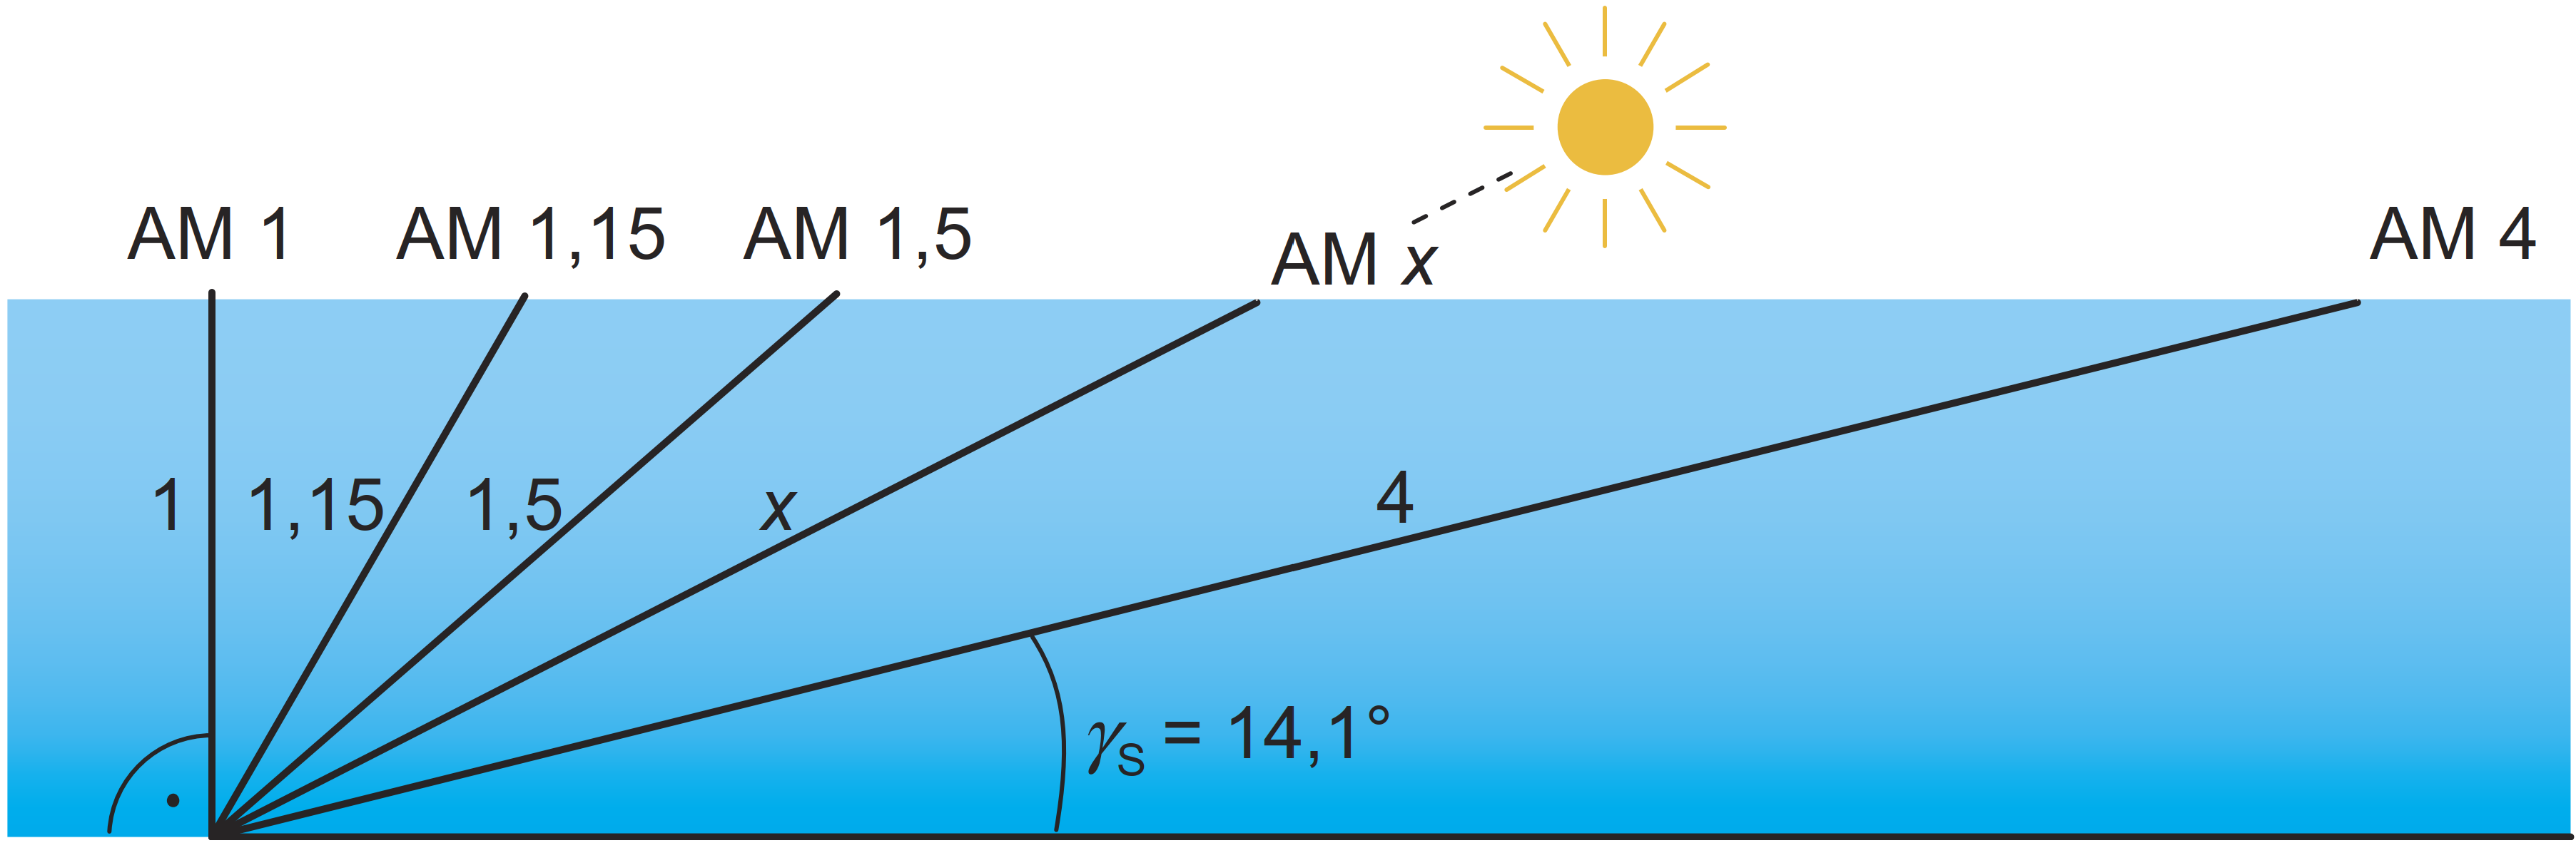
\includegraphics[width=0.95\columnwidth]{images/V01_01.png}

$\boxed{x = \frac{1}{\sin(\gamma_s)}}$

\renewcommand{\arraystretch}{1} % Erhöht Zeilenhöhe für bessere Lesbarkeit
\begin{tabular}{@{} l p {4cm} l @{}}
    [$x$]           & Air Mass Wert         \dotfill & 1            \\
    $[\gamma_{s}]$  & Sonnenstandswinkel    \dotfill & $^\circ$     \\ 
\end{tabular}

\subsection{Solar Spektrum}
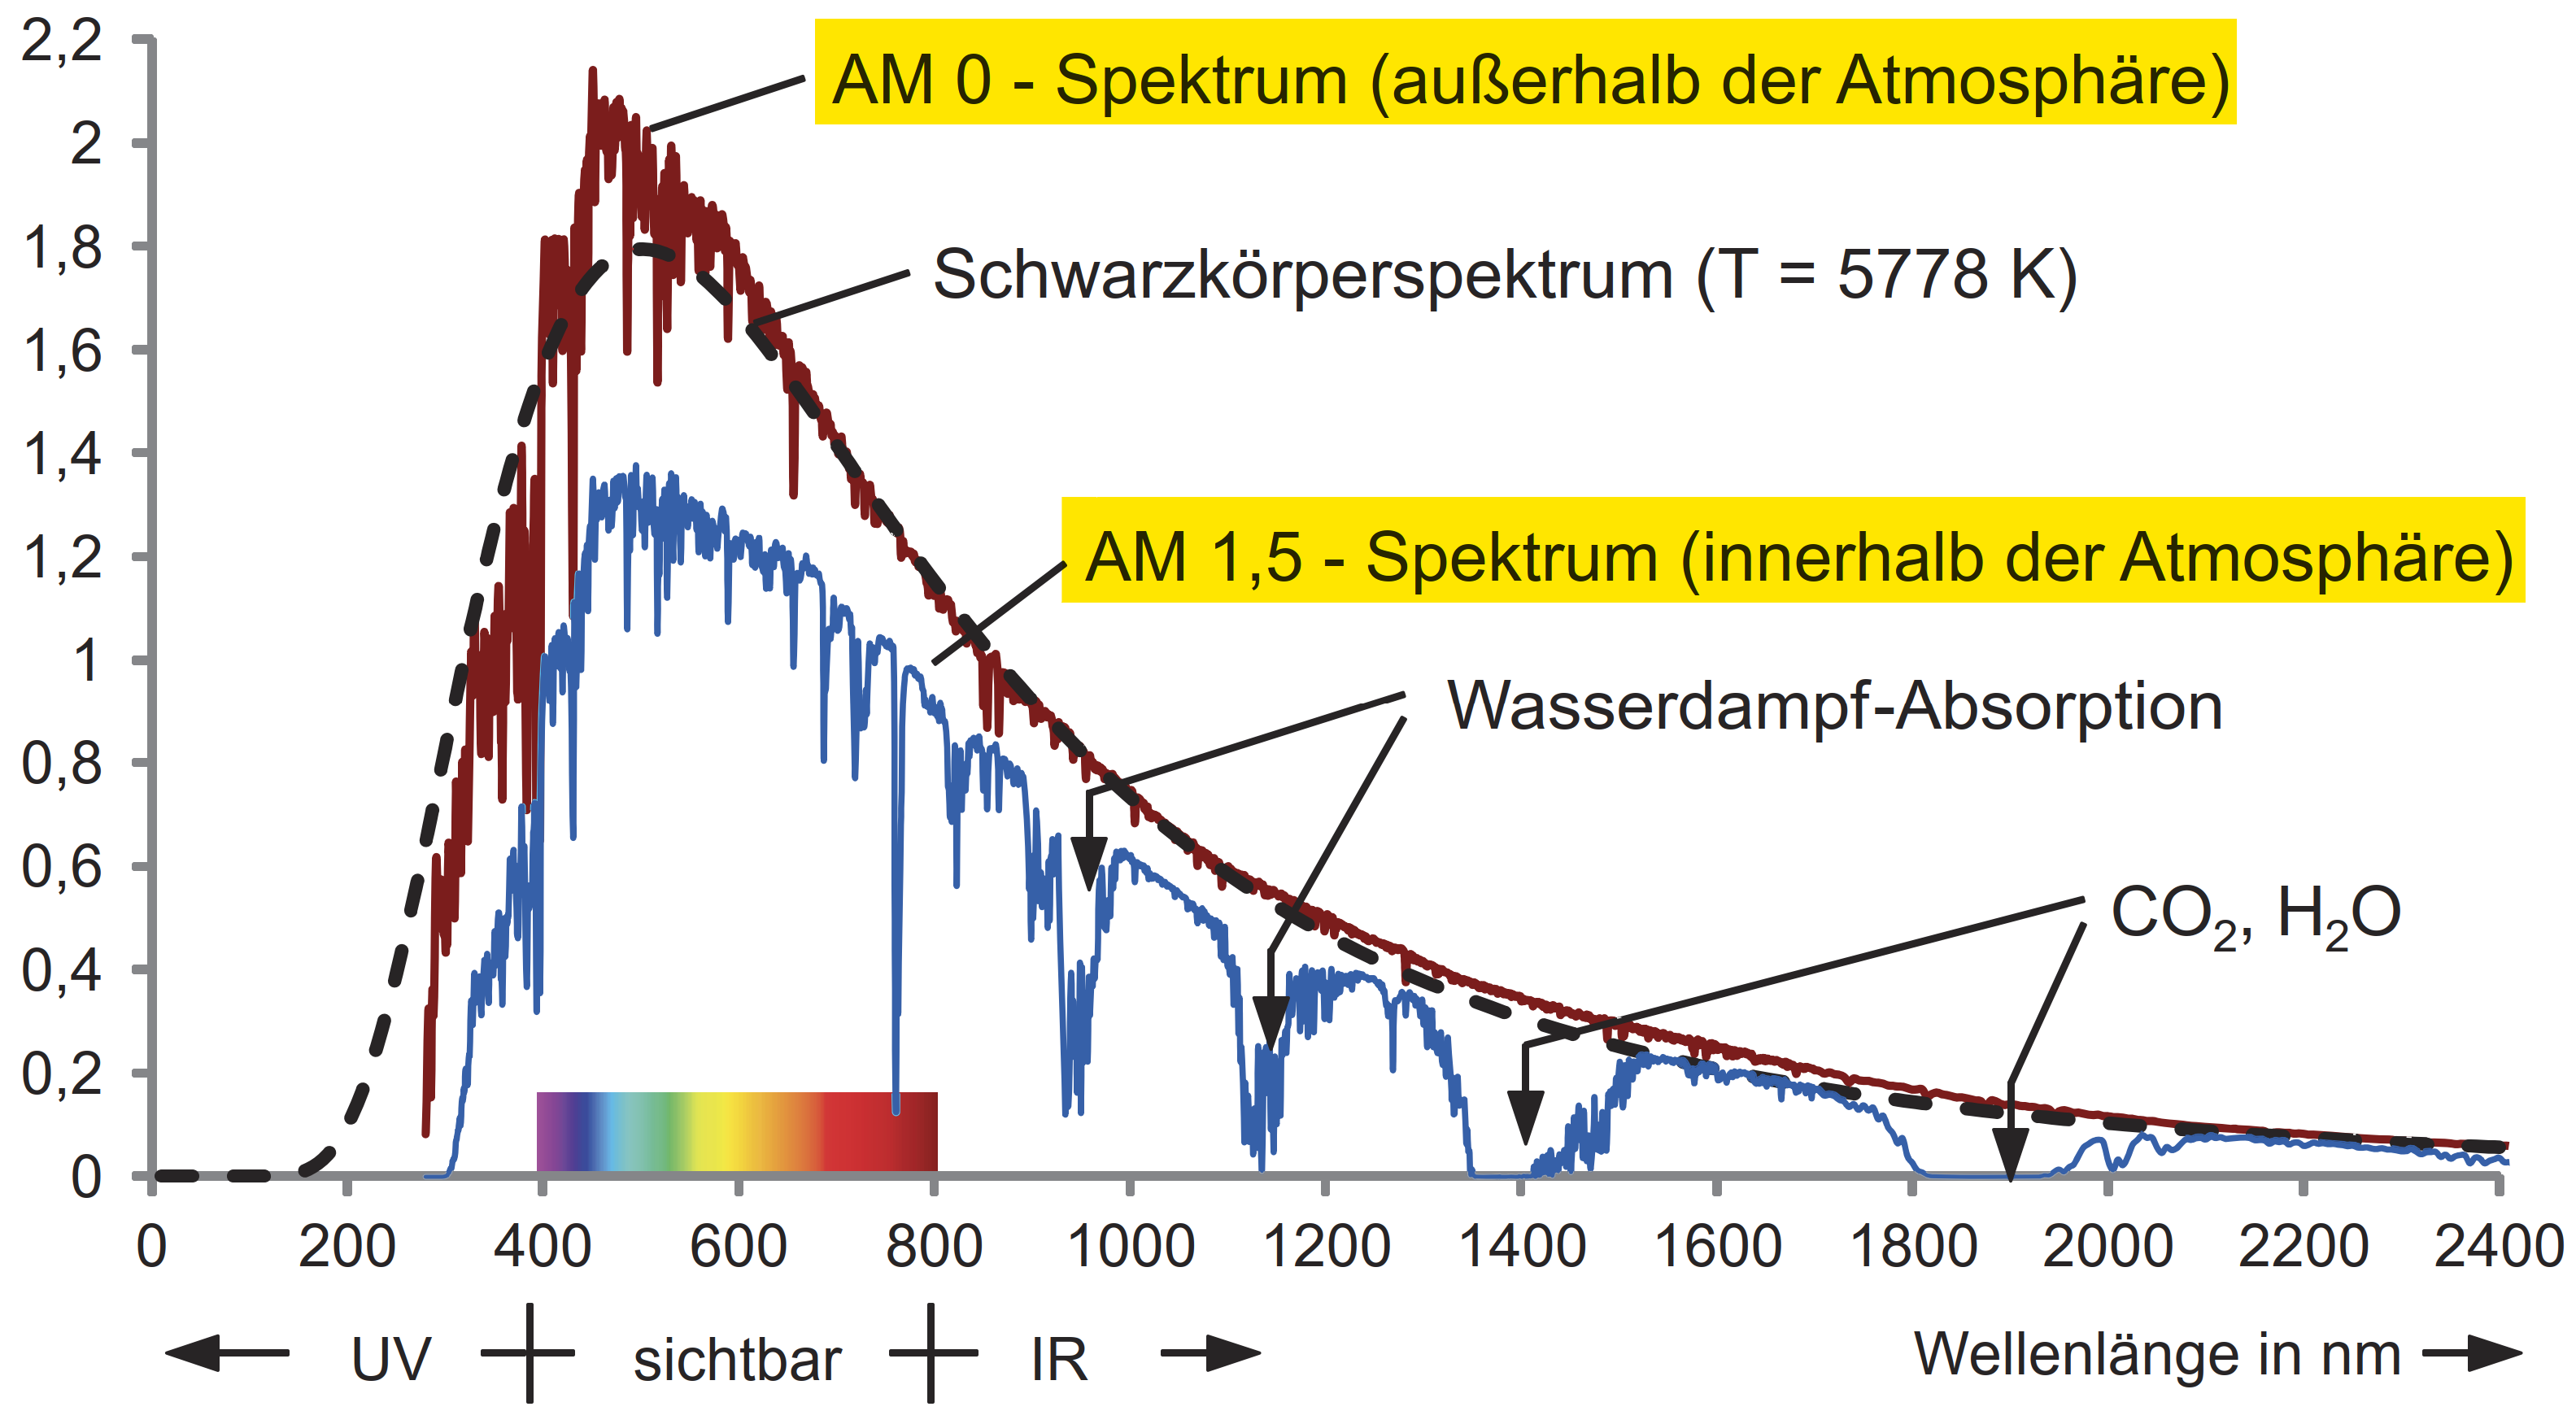
\includegraphics[width=0.95\columnwidth]{images/V01_01.1.png}\\

\renewcommand{\arraystretch}{1.2} % Erhöht Zeilenhöhe für bessere Lesbarkeit
\begin{tabular}{@{} l p {4cm} l @{}}
    $[E_{e,\lambda}]$   & Spektrake Bestrahlungsstärke  \dotfill & $\frac{\watt}{\meter^2 \cdot \text{n} \meter}$ \\
    $[E_{S}]$           & Solarkonstante                \dotfill & $\frac{\watt}{\meter^2}$ \\
    $[\lambda]$         & Wellenlänge                   \dotfill & $\text{n} \meter$ \\ 
\end{tabular}

\subsubsection{Berechnung der Solarkonstante $E_S$}
$E_S = \frac{\text{Strahlungsleistung}}{\text{Kugeloberfläche}}
= \frac{P_{\text{Sonne}}}{4 \cdot \pi \cdot r_{\text{SE}}^2}
= \frac{3{,}845 \cdot 10^{26} \text{ W}}{4 \cdot \pi \cdot (1{,}496 \cdot 10^{11} \text{m})^2}
= 1361 \, \frac{\text{W}}{\text{m}^2}$

\subsection{Global-, Direkt- und Diffusstrahlung}
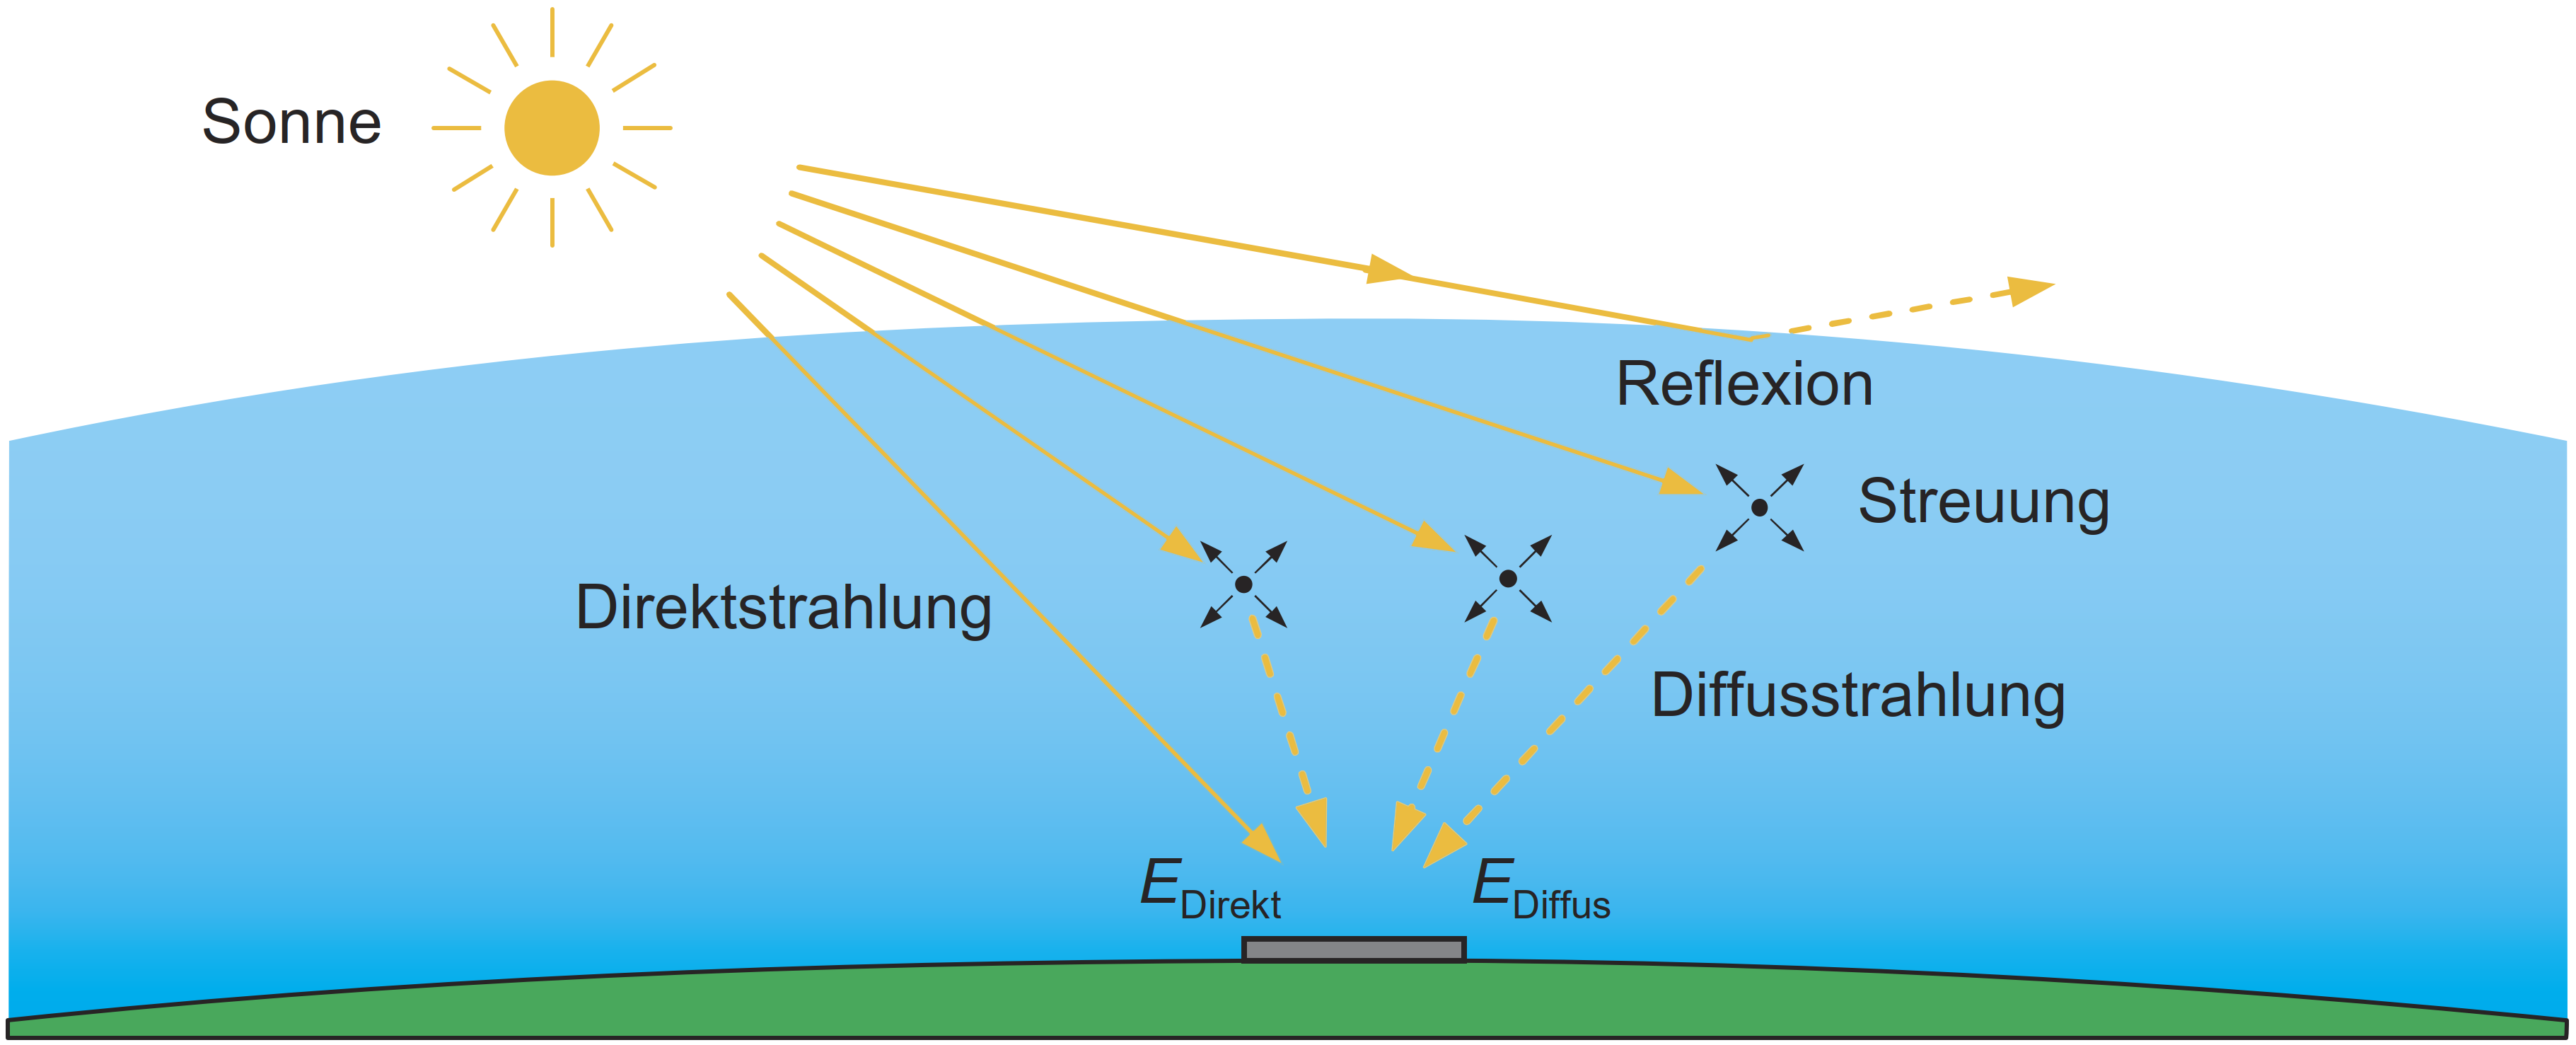
\includegraphics[width=0.95\columnwidth]{images/V01_02.png}

$\boxed{E_G = E_{Dir} + E_{Diff}}$

\renewcommand{\arraystretch}{1.2} % Erhöht Zeilenhöhe für bessere Lesbarkeit
\begin{tabular}{@{} l p {4cm} l @{}}
    $[E_{G}]$       & Globalstrahlung  \dotfill & $\frac{\watt}{\meter^2}$ \\
    $[E_{Dir}]$     & Direktstrahlug   \dotfill & $\frac{\watt}{\meter^2}$ \\
    $[E_{Diff}]$    & Diffusstrahlung  \dotfill & $\frac{\watt}{\meter^2}$ \\ 
\end{tabular}

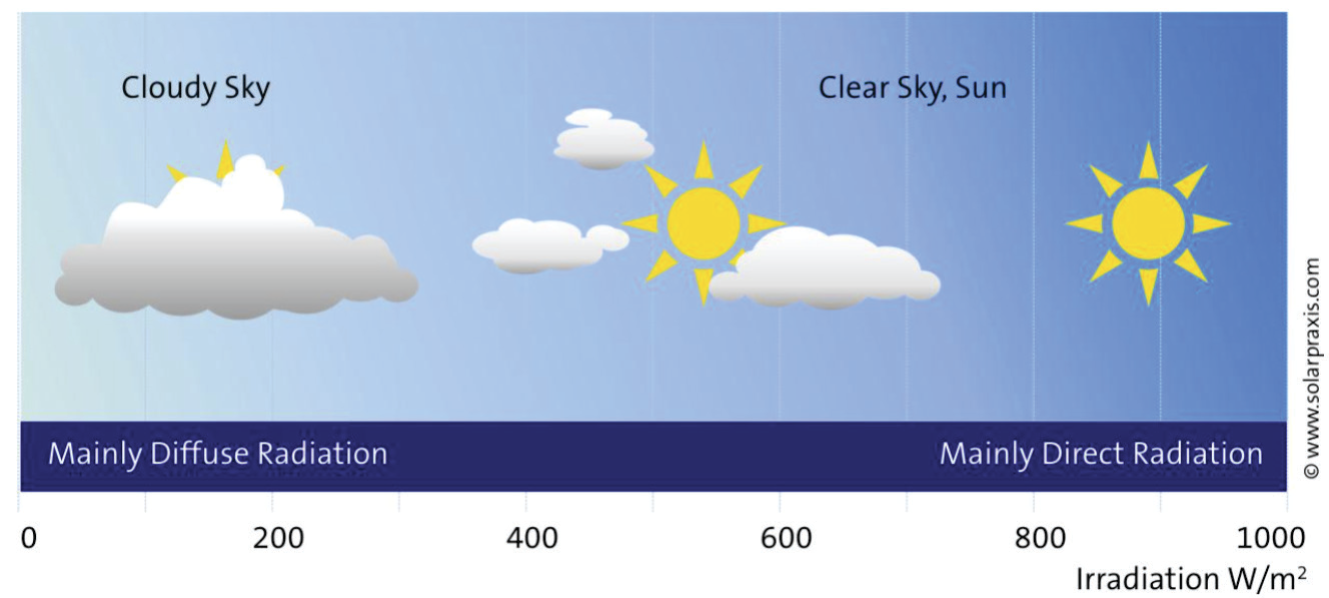
\includegraphics[width=0.65\columnwidth]{images/V01_03.png}




























        \section{Grundlagen Halbleiterphysik}

\subsection{Bohrsches Atommodell}

\myul{\textbf{1. Bohrsches Postulat:}}\\
        Es gibt nur bestimmte diskrete Schalen, die für ein Elektron erlaubt sind.\\
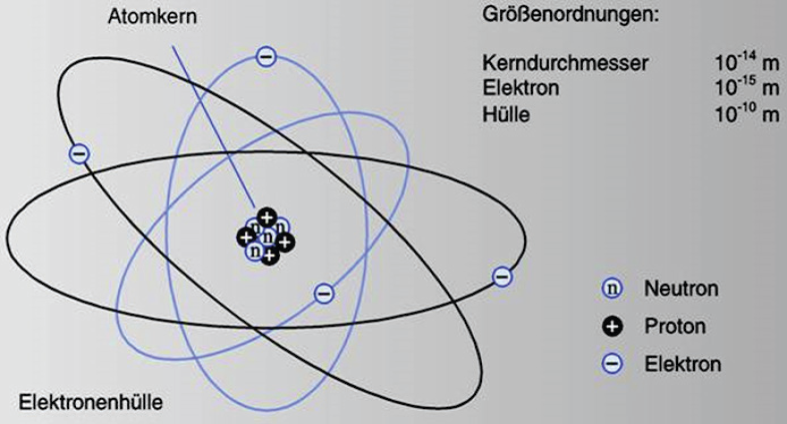
\includegraphics[width=0.95\linewidth]{images/V02_01.png}

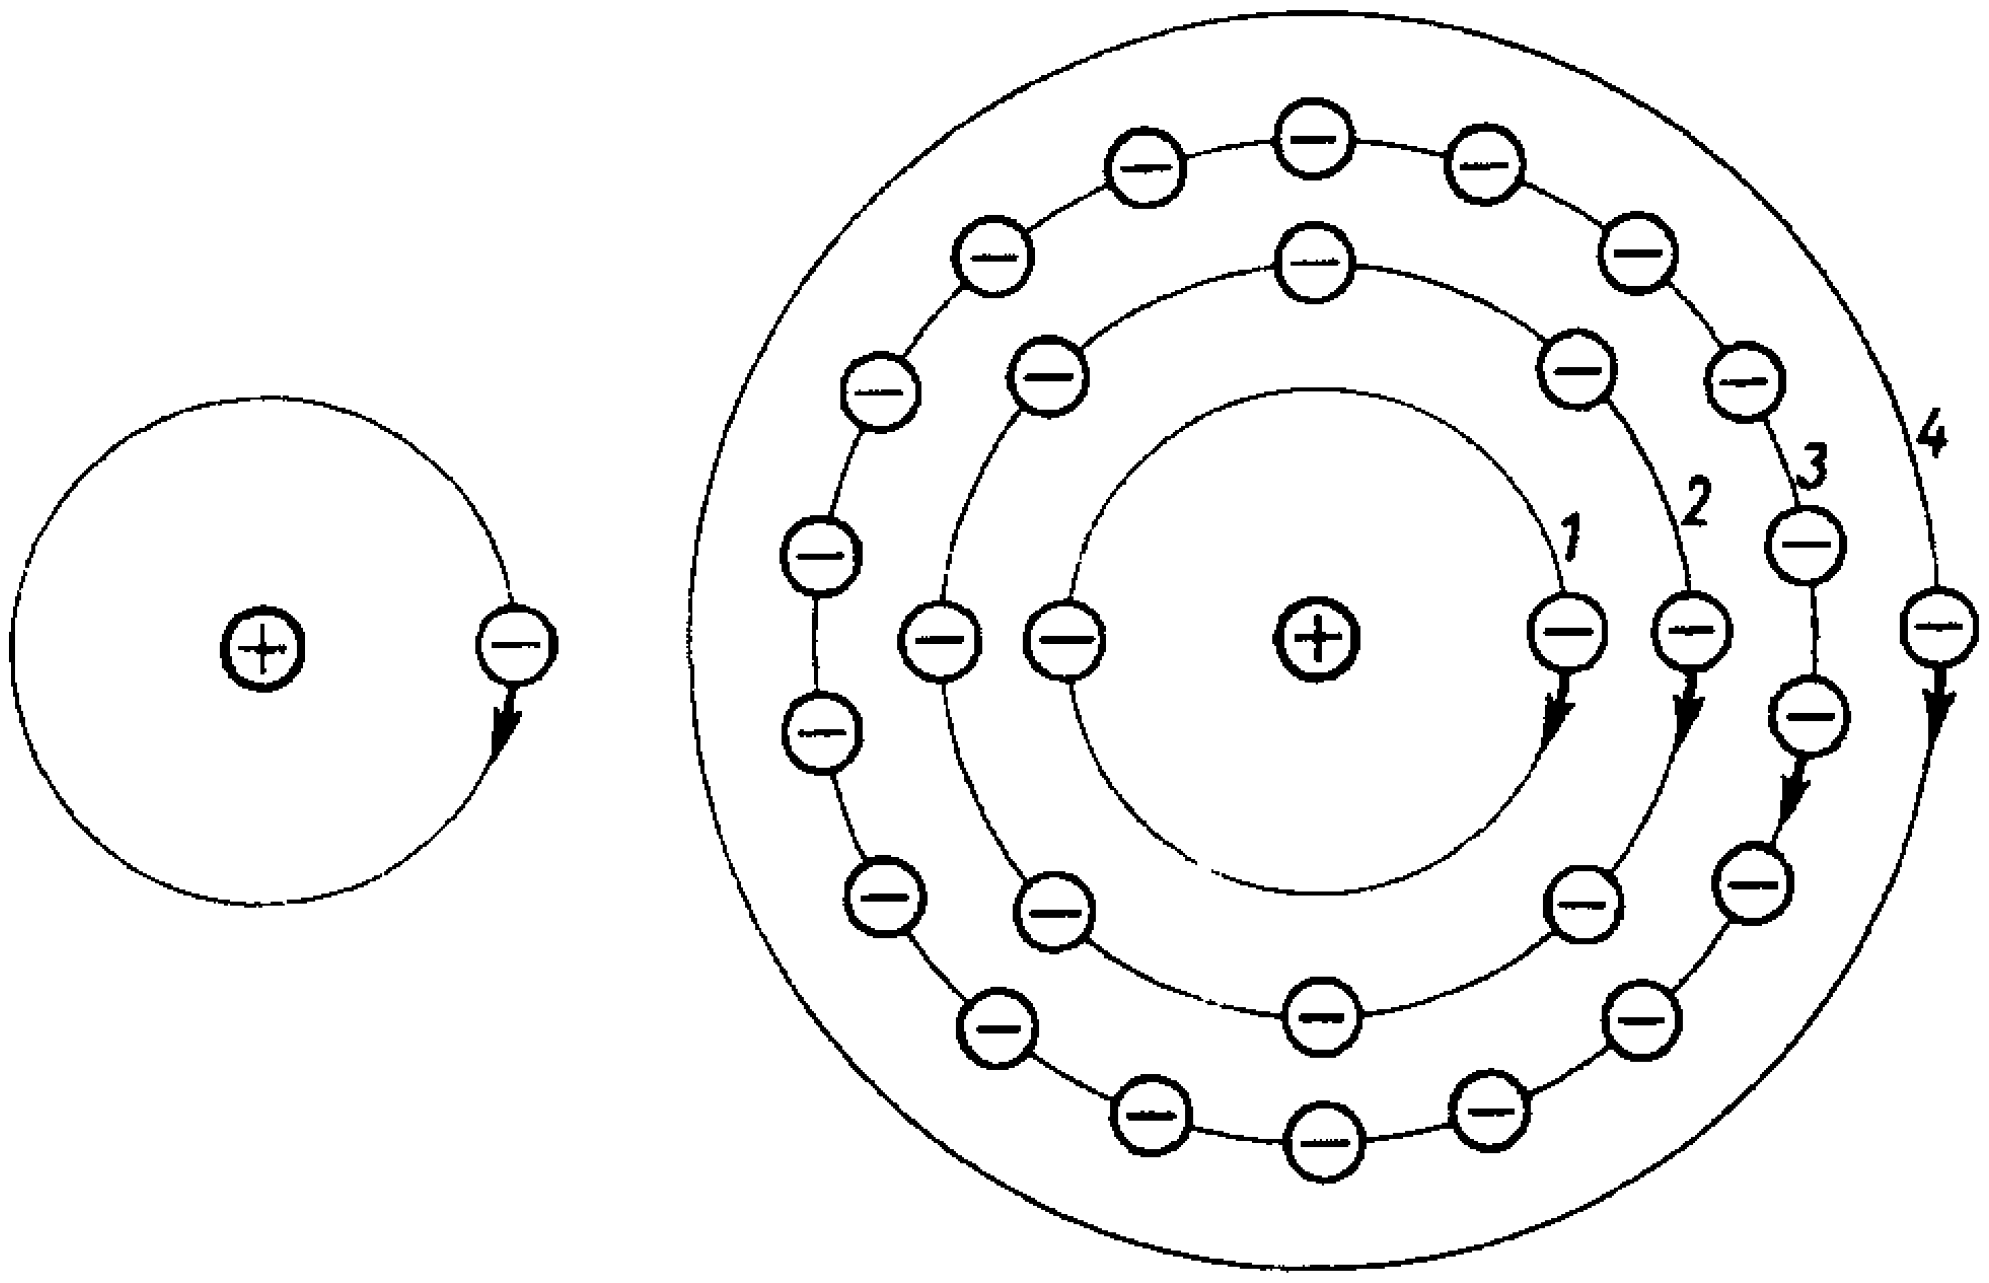
\includegraphics[width=0.75\linewidth]{images/V02_02.png}

Links: Wasserstoff\\
Rechts: Kupfer\\


\renewcommand{\arraystretch}{1.5}
    \begin{tabular}{|l|c|c|}
        \hline
        \textbf{Elementarteilchen} & \textbf{Ruhemasse} & \textbf{Ladung} \\
        \hline
        Proton & $1{,}673 \cdot 10^{-27} \, \text{kg}$ & $+e$ \\
        Neutron & $1{,}675 \cdot 10^{-27} \, \text{kg}$ & $0$ \\
        Elektron & $0{,}911 \cdot 10^{-30} \, \text{kg}$ & $-e$ \\
        \hline
    \end{tabular}

Elementarladung $e = 1.602 \cdot 10^{-19} C$\\



\myul{\textbf{2. Bohrsches Postulat}}\\
Der übergang eines Elektrons von einer Schale zur anderen erfolgt unter Emission der Absorption von elektromagnetischer Strahlung.\\

\begin{minipage}[t]{0.48\columnwidth}
    \textbf{Emission}\\
    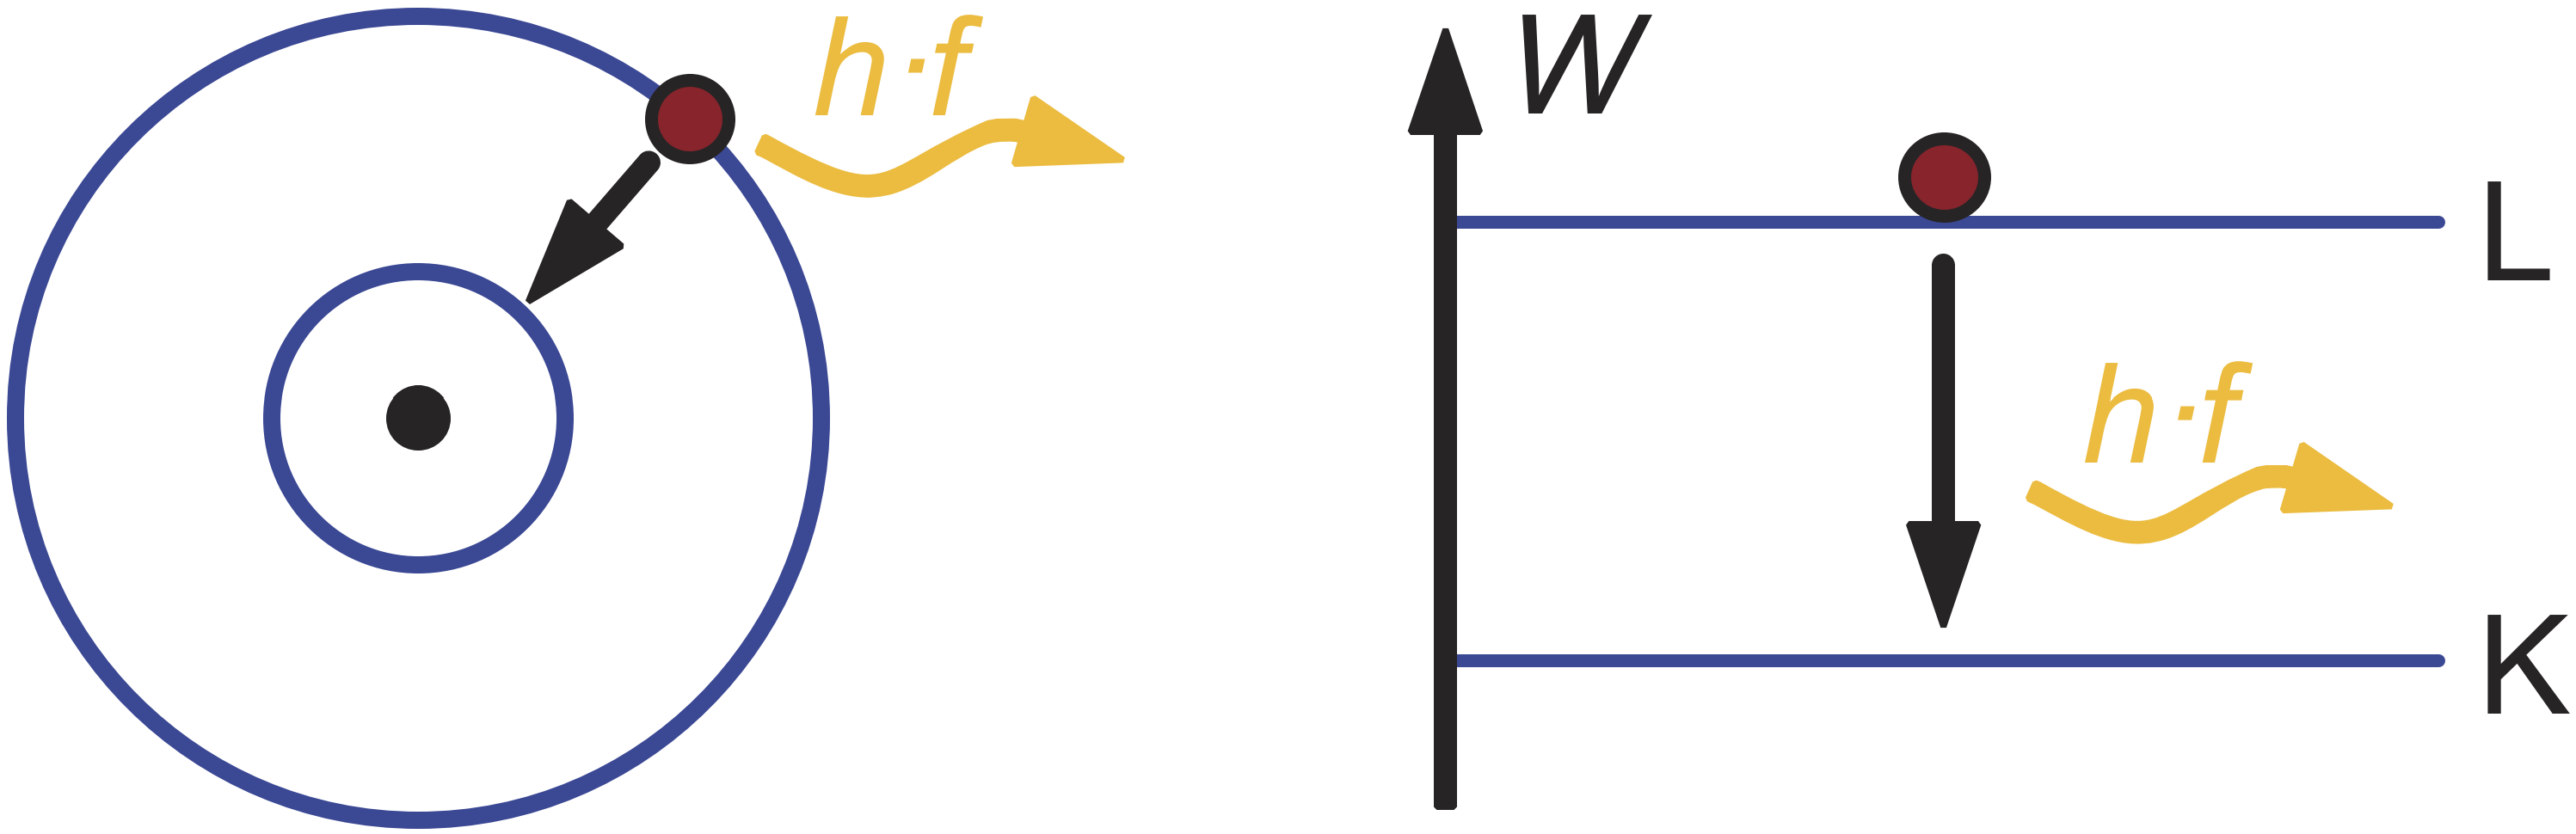
\includegraphics[width=0.85\linewidth]{images/V02_03.png}
\end{minipage}
\hfill
\begin{minipage}[t]{0.48\columnwidth}
    \textbf{Absorption}\\
    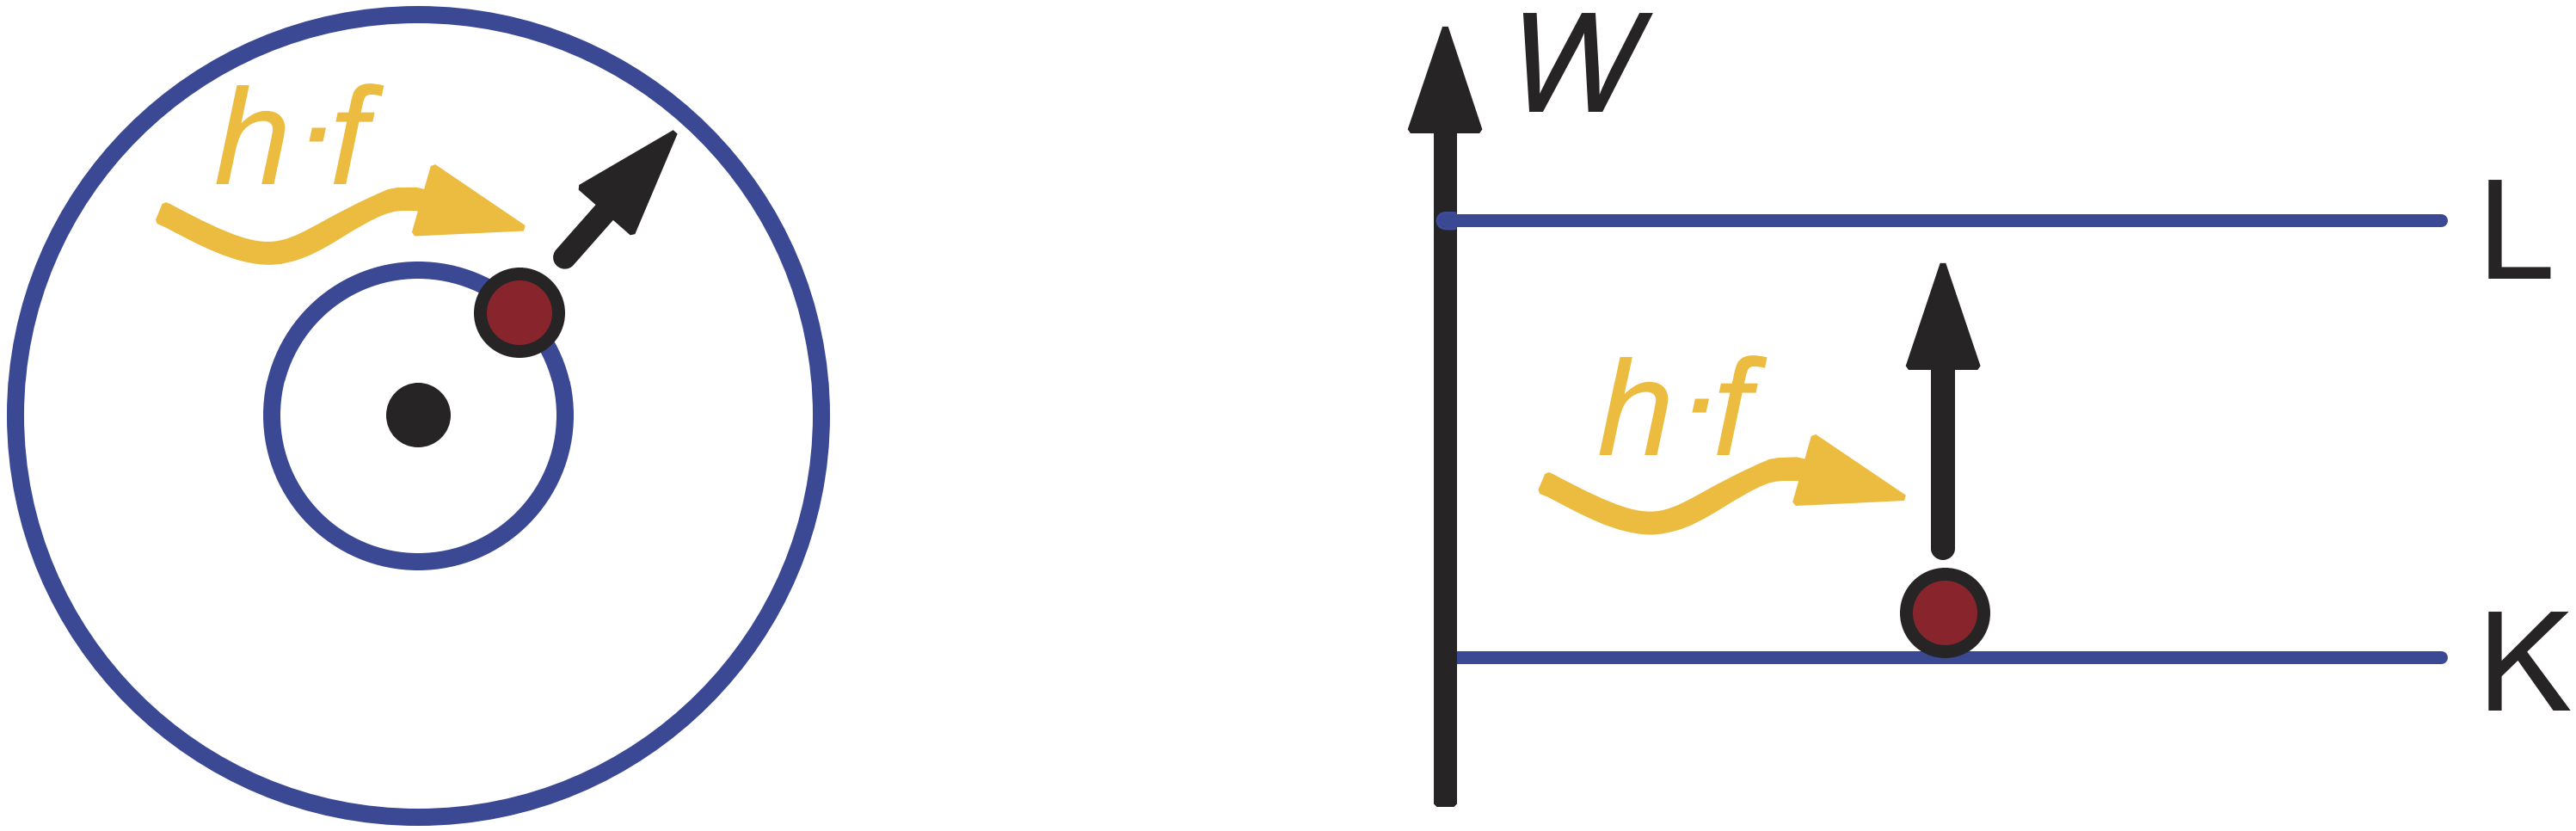
\includegraphics[width=0.85\linewidth]{images/V02_04.png}
\end{minipage}

\vspace{0.5cm}

$\boxed{\Delta W = \lvert W_2 - W_1 \rvert = h \cdot f}$ \quad $\boxed{\lambda = \frac{c_0}{f}}$ \quad $c_0 \approx 3 \cdot 10^8 \frac{m}{s}$

\renewcommand{\arraystretch}{1.2} % Erhöht Zeilenhöhe für bessere Lesbarkeit
\begin{tabular}{@{} l p {4cm} l @{}}
    $[\Delta W]$    & Energiedifferenz          \dotfill & $Ws$ \\
    $[W_1]$         & Energie vor dem Übergang  \dotfill & $Ws$ \\
    $[W_2]$         & Energie nach dem Übergang \dotfill & $Ws$ \\
    $[h]$           & Plancksches Wirkungsquantum \dotfill & $Ws^2$ \\
    $[f]$           & Frequenz \dotfill & $\frac{1}{s}$ \\
    $[c_0]$         & Lichtgeschwindigkeit \dotfill & $\frac{m}{s}$ \\
    $[\Lambda]$     & Wellenlänge \dotfill & $m$ \\
\end{tabular}
































        \section{Solarzelle}

\subsection{Aufbau Solarzelle}

\begin{center}
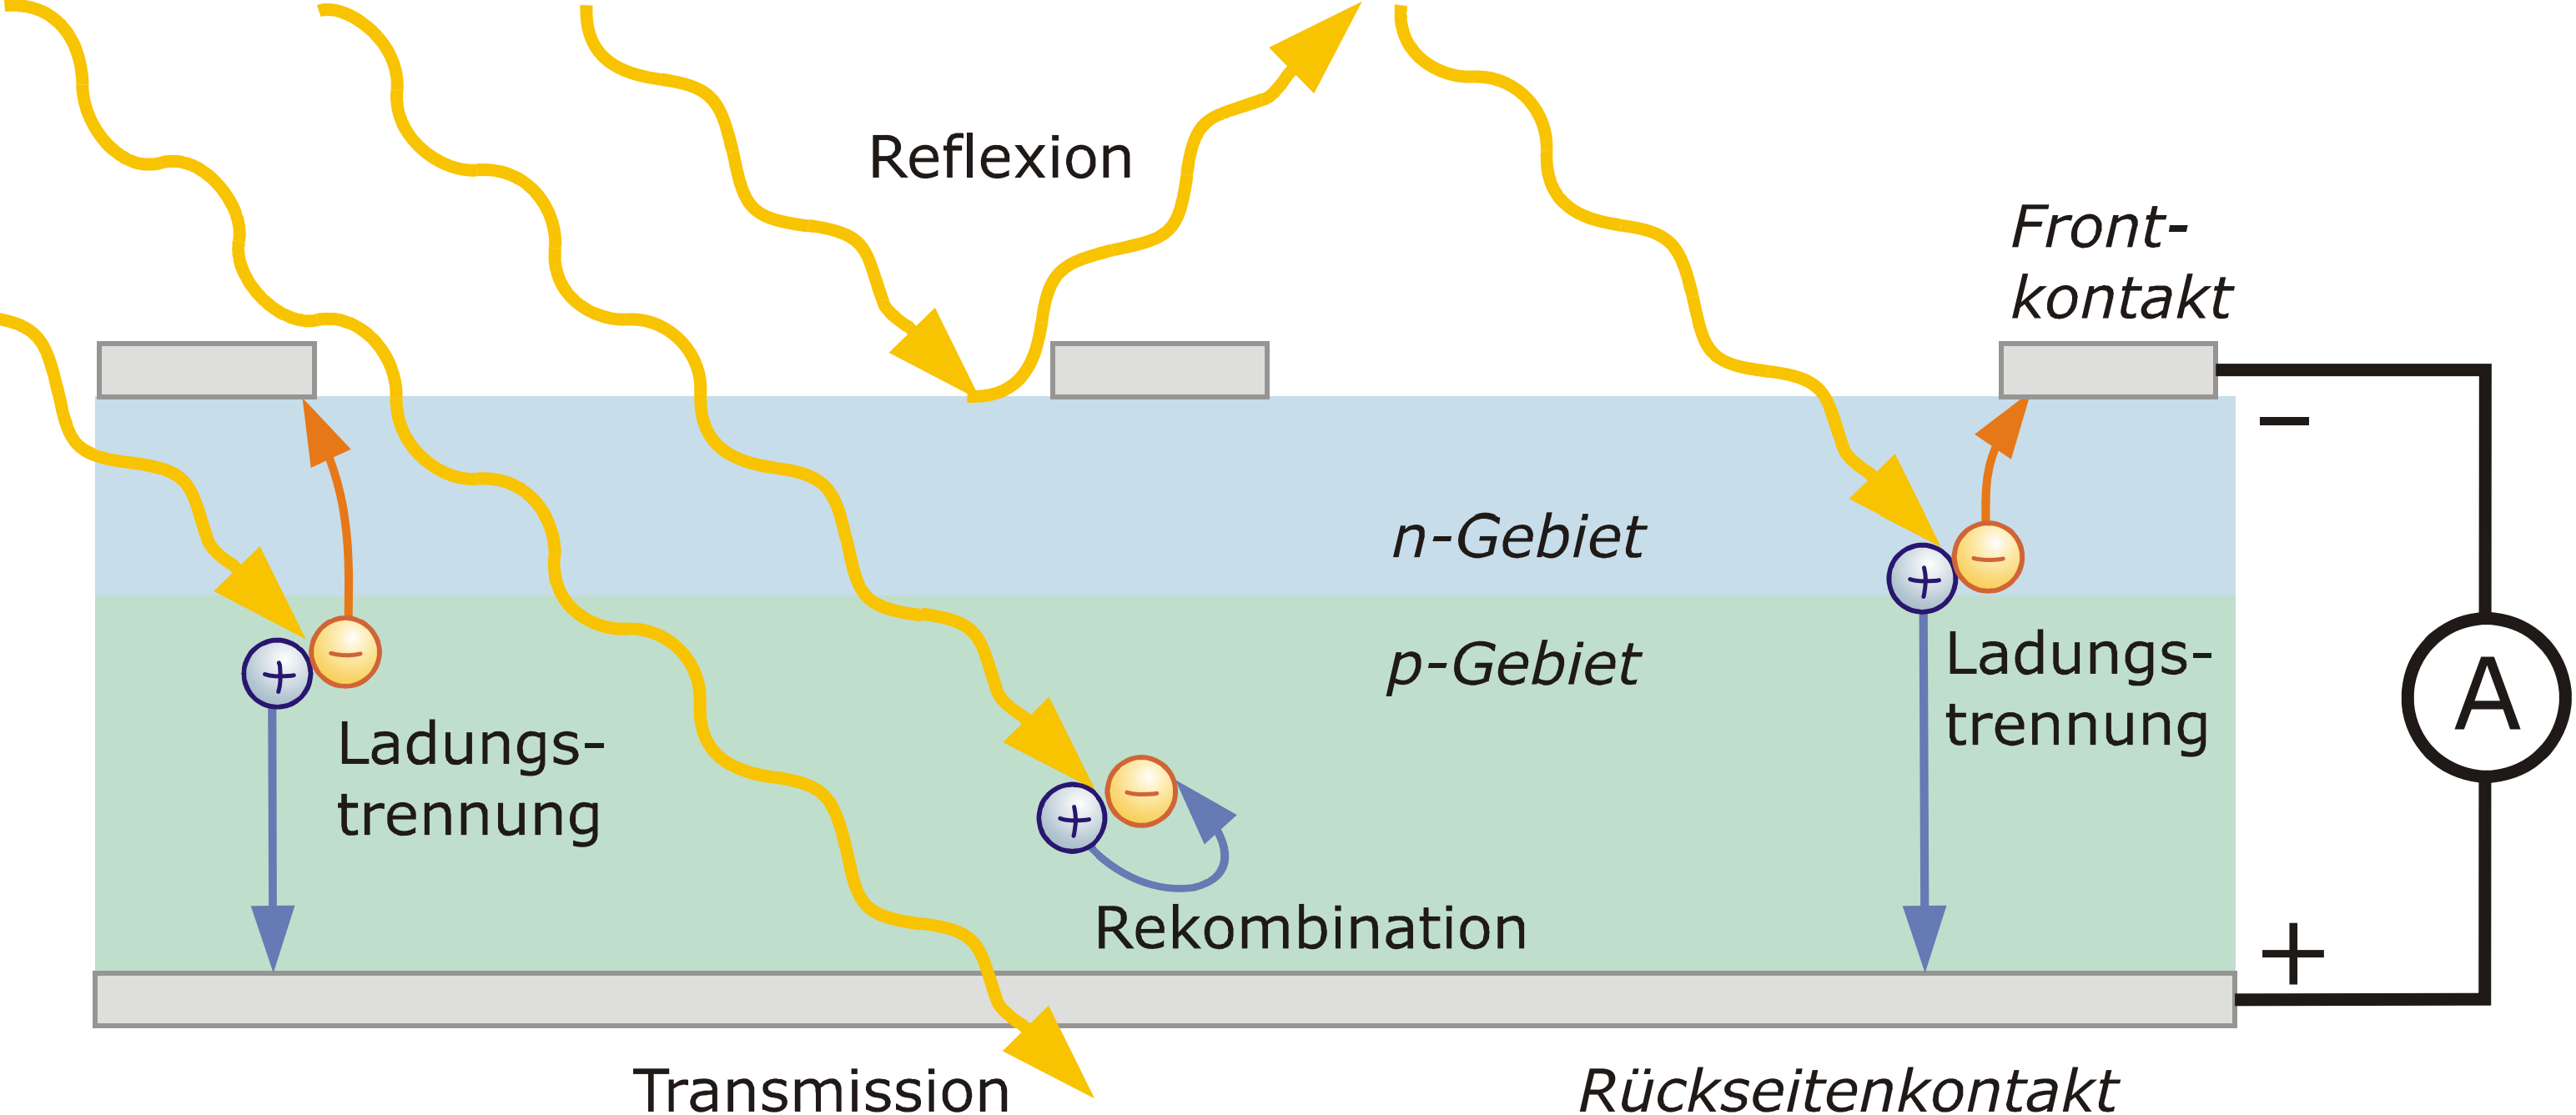
\includegraphics[width=0.8\linewidth]{images/Solarzelle_bei_Bestrahlung.png}
\end{center}

%\begin{center}
%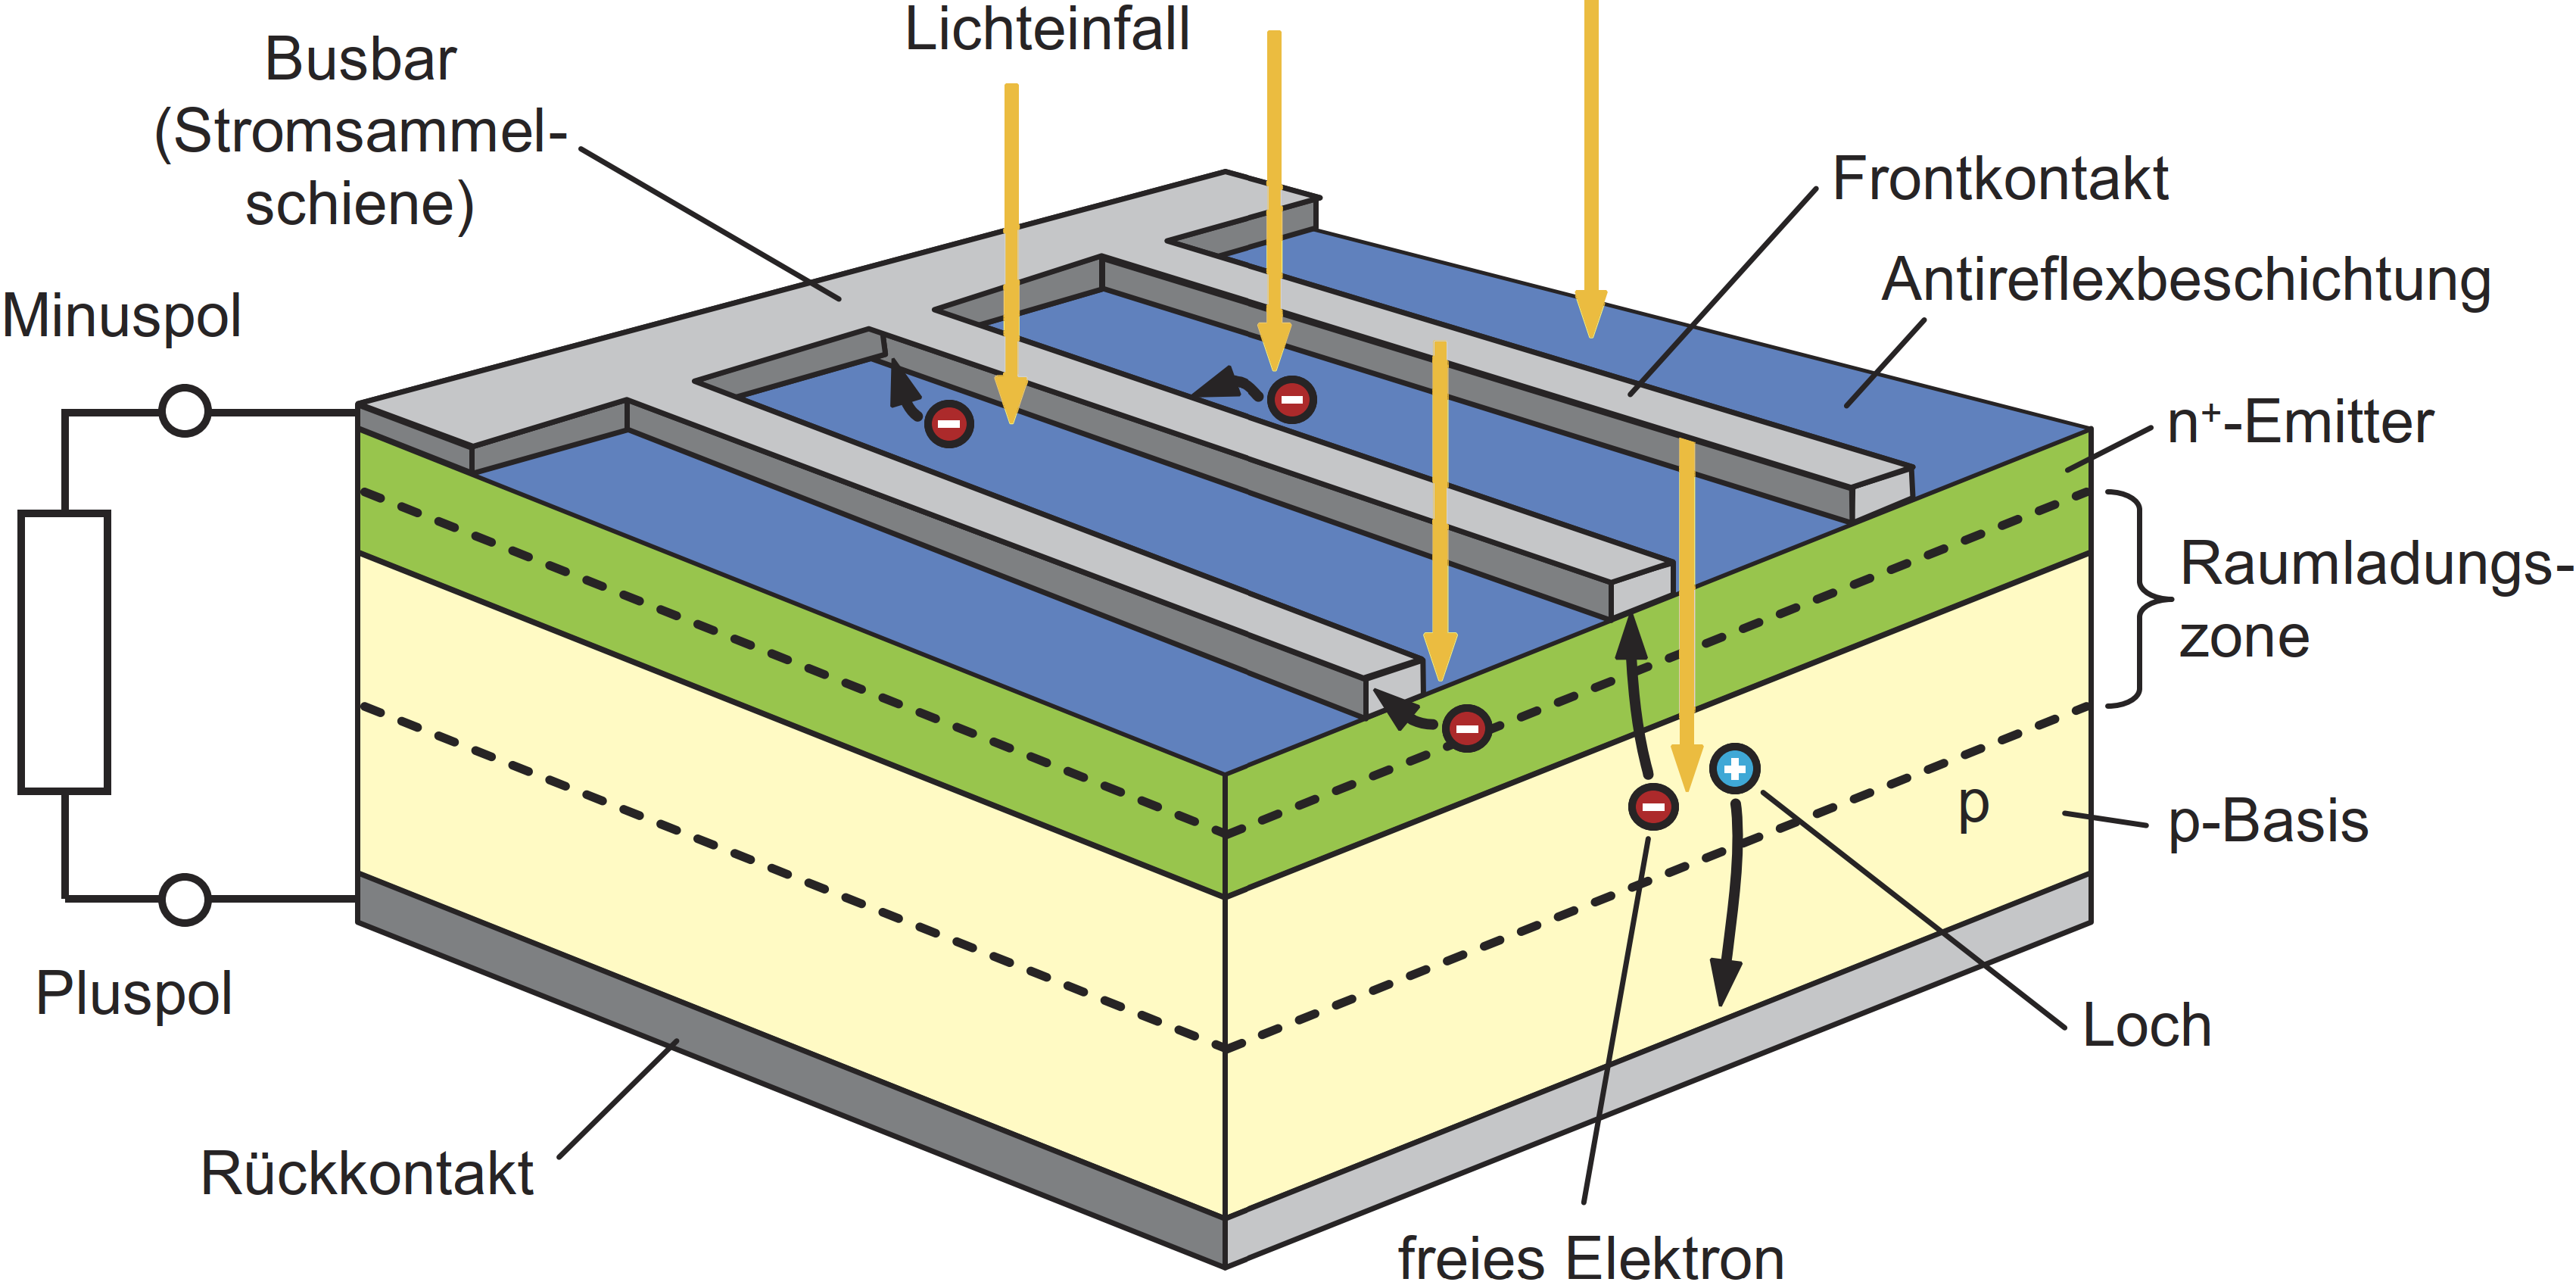
\includegraphics[width=0.9\linewidth]{images/Aufbau_Solarzelle.png}
%\end{center}

\subsection{Reflexionsfaktor}

\begin{minipage}[c]{0.2\columnwidth}
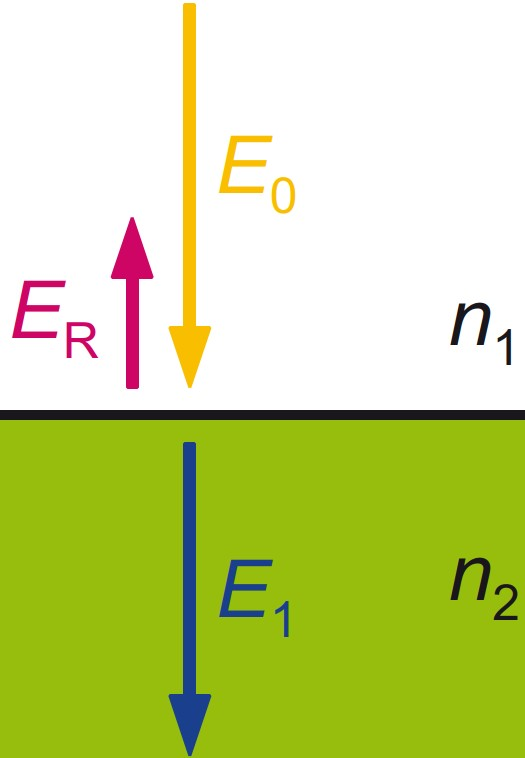
\includegraphics[width=0.98\linewidth]{images/Regflexion.jpg}
\end{minipage}
\hfill
\begin{minipage}[c]{0.78\columnwidth}

    $\boxed{R=\left (\frac{n_1-n_2}{n_1+n_2}\right)^2}
    \quad
    \boxed{R = \frac{E_{\mathrm{R}}}{E_{\mathrm{0}}}}
    $

    \vspace{0.1cm}

    \renewcommand{\arraystretch}{1.2}
    \begin{tabular}{@{} l p{5.5cm} l @{}}
        $[R]$                   & Reflexionsfaktor  \dotfill & $\mathrm{-}$ \\
        $[n_1]$                 & Brechungsindex 1 (Luft = 1)  \dotfill & $\mathrm{-}$ \\
        $[n_2]$                 & Brechungsindex 2  \dotfill & $\mathrm{-}$ \\
        $[E_{\mathrm{0}}]$      & Einfallende Strahlungsstärke  \dotfill & $\frac{\mathrm{W}}{\mathrm{m^2}}$\\
        $[E_{\mathrm{R}}]$      & Reflektierte Strahlungsstärke \dotfill & $\frac{\mathrm{W}}{\mathrm{m^2}}$
    \end{tabular}
\end{minipage}




\subsection{Quantenwirkungsgrad}



\subsubsection{Externer Quantenwirkungsgrad $\eta_{\mathrm{Ext}}$}

Nicht alle erzeugten Elektron-Loch-Paare tragen zum Photostrom bei. Daher definiert man den externen Quantenwirkungsgrad \( \eta_\text{Ext} \) als das Verhältnis der für den Photostrom nutzbaren Elektron-Loch-Paare zu den insgesamt auftreffenden Photonen.

\vspace{0.1cm}

\begin{minipage}[t]{0.2\columnwidth}
$
\boxed{\eta_{\text{Ext}} = \frac{N_{ELP}}{N_{Ph}}}
$
\end{minipage}
\hfill
\begin{minipage}[t]{0.78\columnwidth}
    \renewcommand{\arraystretch}{1.2}
\begin{tabular}{@{} l p{5.5cm} l @{}}
    $[\eta_{\mathrm{Ext}}]$   & Externer Quantenwirkungsgrad  \dotfill & $\mathrm{-}$ \\
    $[N_{\mathrm{ELP}}]$    & Anzahl nutzbarer Elektronen-Loch-Paare        \dotfill & $\mathrm{-}$ \\
    $[N_{\mathrm{Ph}}]$       & Anzahl auftretender Photonen  \dotfill & $\mathrm{-}$ \\
\end{tabular}
\end{minipage}


\subsubsection{Interner Quantenwirkungsgrad $\eta_{\mathrm{Int}}$}

Neben dem externen definiert man auch den internen Quantenwirkungsgrad \( \eta_\text{Int} \), bei dem die durch Reflexion verursachten Verluste herausgerechnet werden.

\vspace{0.1cm}


\begin{minipage}[t]{0.2\columnwidth}
$
\boxed{\eta_{\text{Int}} = \frac{\eta_{\text{Ext}}}{1 - R}}
$
\end{minipage}
\hfill
\begin{minipage}[t]{0.78\columnwidth}
    \renewcommand{\arraystretch}{1.2}
\begin{tabular}{@{} l p{5.5cm} l @{}}
    $[\eta_{\mathrm{Int}}]$   & Interner Quantenwirkungsgrad  \dotfill & $\mathrm{-}$ \\
    $[\eta_{\mathrm{Ext}}]$   & Externer Quantenwirkungsgrad  \dotfill & $\mathrm{-}$ \\
    $[R]$                     & Reflexionsfaktor  \dotfill & $\mathrm{-}$ \\
\end{tabular}
\end{minipage}



\subsection{Rekombination}

Rekombination bezeichnet den Prozess, bei dem Elektronen und Löcher in einem Halbleiter wieder zusammenfinden und dabei ihre Energie abgeben. Dies kann durch Wärme oder Lichtemission geschehen.

\vspace{0.1cm}

\begin{itemize}
  \item Störstellenrekombination an Fremdatomen oder Kristallfehlern
  \item Oberflächenrekombination
\end{itemize}

\vspace{0.1cm}

\textbf{Diffusionslänge} \( L_N \) Silizium: 50 -- 500\,µm



\subsection{Lichtabsorbtion, Bestrahlungsstärke und Eindringtiefe}

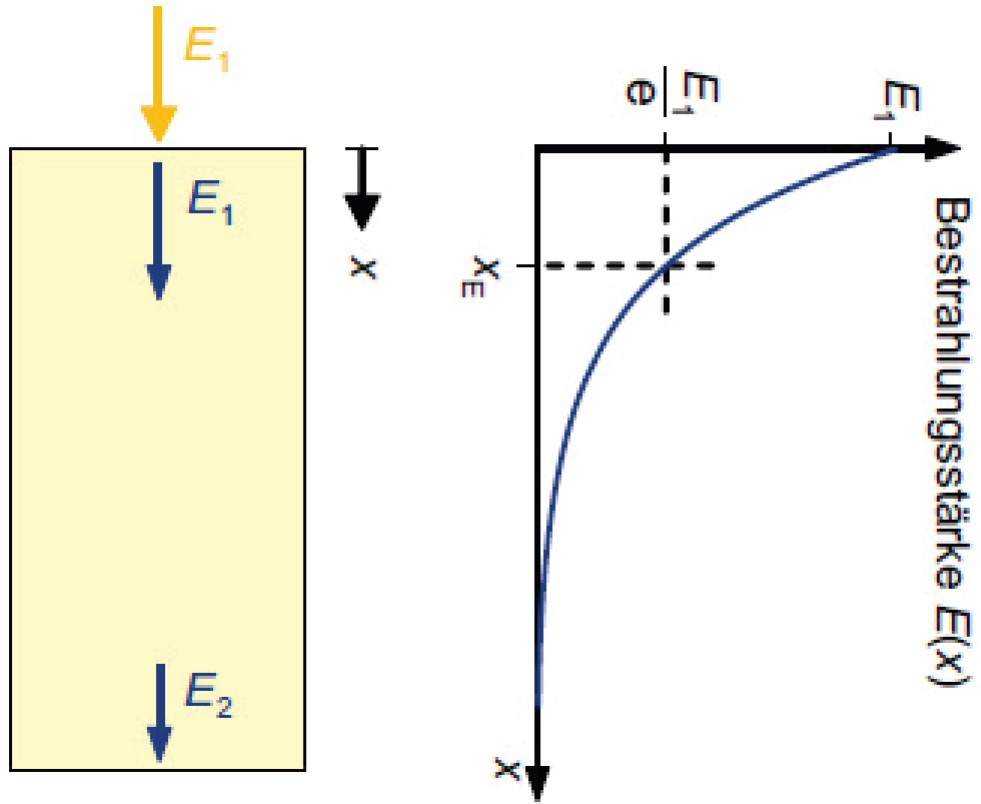
\includegraphics[width=0.6\linewidth]{images/Lichtabsorption.jpg}

\vspace{0.1cm}

$
\boxed{
E(x) = E_1 \cdot e^{-\alpha \cdot x}
}
\quad
\boxed{
x_\mathrm{E} = \frac{1}{\alpha}
}
$

\vspace{0.1cm}

\renewcommand{\arraystretch}{1.2}
\begin{tabular}{@{} l p{6.5cm} l @{}}
    $[E(x)]$      & Bestrahlungsstärke in Tiefe $x$ \dotfill & $\frac{\mathrm{W}}{\mathrm{m^2}}$ \\
    $[E_1]$       & Bestrahlungsstärke an der Oberfläche ($x=0$) \dotfill & $\frac{\mathrm{W}}{\mathrm{m^2}}$ \\
    $[\alpha]$    & Absorptionskoeffizient \dotfill & $\frac{\mathrm{1}}{\mathrm{m}}$ \\
    $[x]$         & Eindringtiefe \dotfill & $\mathrm{m}$ \\
    $[x_\mathrm{E}]$ & Eindringtiefe des Lichts \dotfill & $\mathrm{m}$ \\
\end{tabular}


\subsection{Absorptionswirkungsgrad}

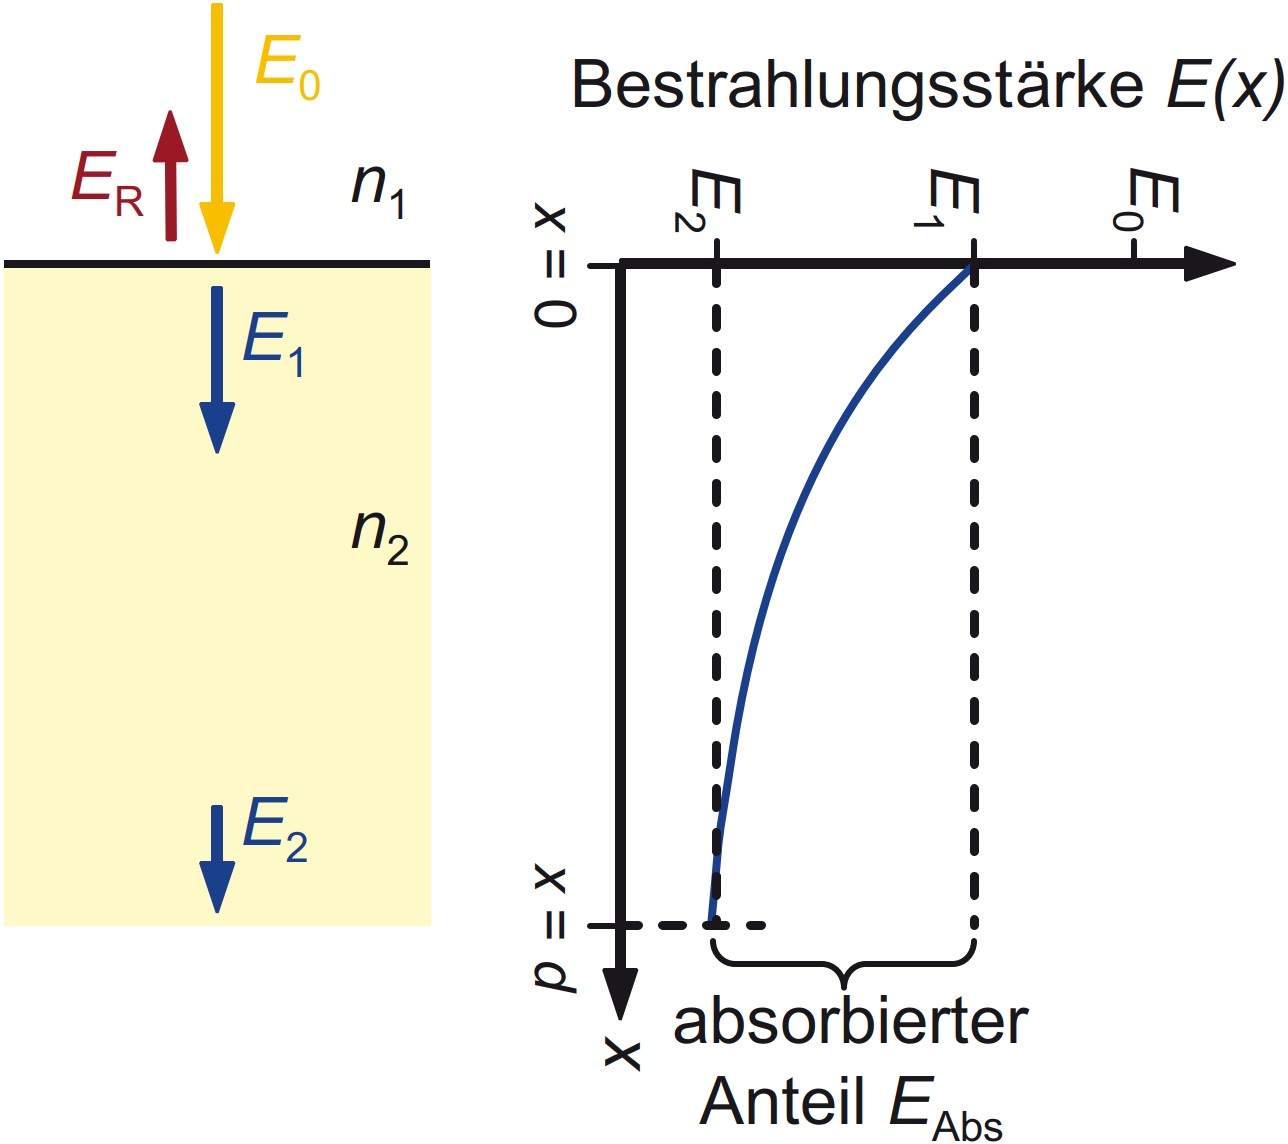
\includegraphics[width=0.6\linewidth]{images/Absorptionswirkungsgrad.jpg}

\vspace{0.1cm}

Wir definieren den Absorptionswirkungsgrad $\eta_\mathrm{Abs}$ als das Verhältnis der Zahl der absorbierten Photonen zur Zahl der aussen auftreffenden Photonen:

\vspace{0.1cm}

$
\boxed{
\eta_\mathrm{Abs} = \frac{N_\mathrm{Ph\_Abs}}{N_\mathrm{Ph}}
}
$
$
\boxed{
\eta_\mathrm{Abs} =  \frac{E_\mathrm{Abs}}{E_0}
}
$
$
\boxed{
\eta_\mathrm{Abs}  \frac{E_1 - E_2}{E_0}
}
$
$
\boxed{
\eta_\mathrm{Abs} = (1 - R) \cdot \left(1 - \mathrm{e}^{-\alpha \cdot d} \right)
}
$

$
\boxed{
E_{1} = (1 - R) \cdot E_0
}
$
$
\boxed{
E_{2} = E_1 \cdot e^{- \alpha \cdot d}
}
$

\vspace{0.1cm}

\renewcommand{\arraystretch}{1.2}
\begin{tabular}{@{} l p{6.5cm} l @{}}
    $[\eta_{\mathrm{Abs}}]$   & Absorptionswirkungsgrad  \dotfill & $\mathrm{-}$ \\
    $[N_\mathrm{Ph}]$ & Anzahl auftretender Photonen \dotfill & - \\
    $[N_\mathrm{Ph\_Abs}]$ & Anzahl absorbierter Photonen \dotfill & - \\
    $[E_{\mathrm{Abs}}]$      & Absorbierte Strahlungsstärke  \dotfill & $\frac{\mathrm{W}}{\mathrm{m^2}}$\\
    $[E_{\mathrm{0}}]$      & Einfallende Strahlungsstärke  \dotfill & $\frac{\mathrm{W}}{\mathrm{m^2}}$\\
    $[E_{\mathrm{1}}]$      & Strahlungsstärke bei x = 0  \dotfill & $\frac{\mathrm{W}}{\mathrm{m^2}}$\\
    $[E_{\mathrm{2}}]$      & Strahlungsstärke bei x = d  \dotfill & $\frac{\mathrm{W}}{\mathrm{m^2}}$\\
    $[R]$         & Reflexionsfaktor \dotfill & - \\
    $[\alpha]$    & Absorptionskoeffizient \dotfill & $\frac{\mathrm{1}}{\mathrm{m}}$ \\
    $[d]$         & Eindringtiefe (Schichtdicke) \dotfill & $\mathrm{m}$ \\ 
\end{tabular}




\subsection{Diodengleichung (Shockley-Gleichung)}

$
\boxed{
I = I_\text{S} \cdot \left( e^{\frac{U}{U_\text{T}}} - 1 \right)
}
\quad
\boxed{
U_\text{T} = \frac{k \cdot T}{q}
}
\qquad 
k \approx 1.38 \cdot 10^{-23} \, \mathrm{\frac{J}{K}}
\qquad
q \approx 1.602 \cdot 10^{-19} \, \mathrm{C}
$

\vspace{0.1cm}

\renewcommand{\arraystretch}{1.2}
\begin{tabular}{@{} l p{6.5cm} l @{}}
    
    
\end{tabular}

\begin{minipage}[t]{0.48\columnwidth}
    \renewcommand{\arraystretch}{1.2}
    \begin{tabular}{@{} l p{2.9cm} l @{}}
        $[I]$           & Diodenstrom \dotfill                 & $\mathrm{A}$ \\
        $[I_\text{S}]$  & Sättigungsstrom \dotfill             & $\mathrm{A}$ \\
        
    \end{tabular}
\end{minipage}
\hfill
\vrule width 1pt
\hfill
\begin{minipage}[t]{0.48\columnwidth}
    \renewcommand{\arraystretch}{1.2}
    \begin{tabular}{@{} l p{3.1cm} l @{}}
        $[U]$           & anliegende Spannung \dotfill                   & $\mathrm{V}$ \\
        $[U_\text{T}]$  & Temperaturspannung \dotfill                    & $\mathrm{V}$ \\
    \end{tabular}
\end{minipage}



\subsection{Solarzelle}
\subsubsection{Vereinfachtes Modell}

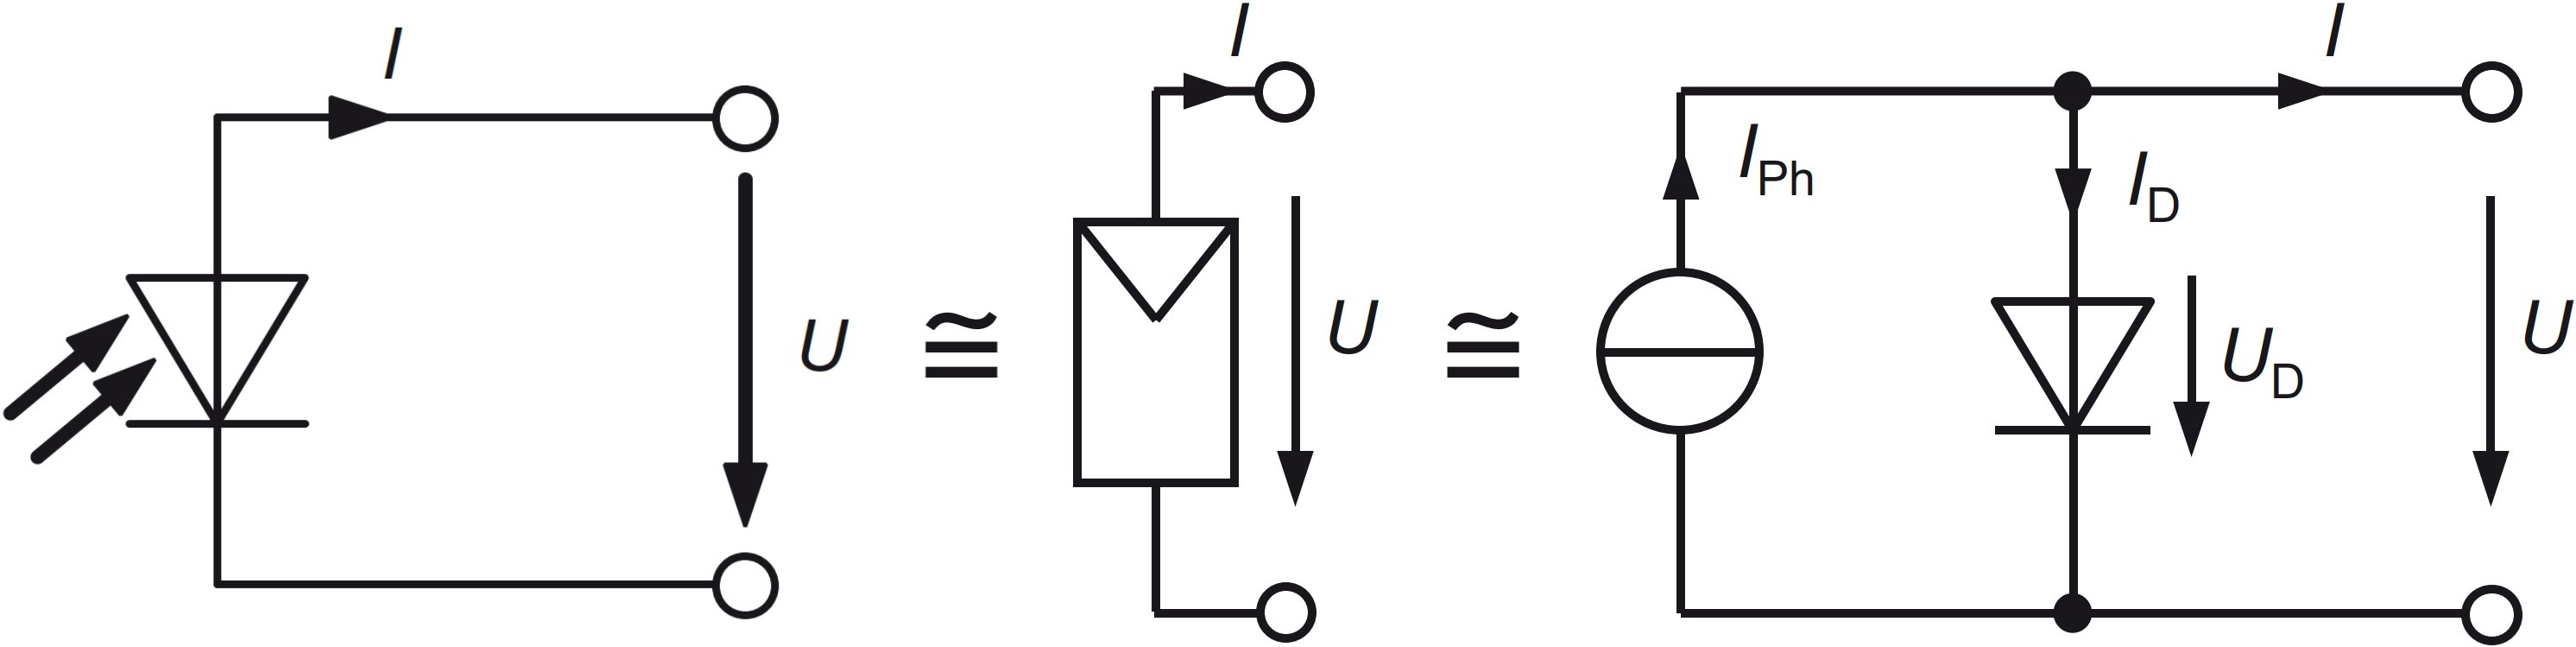
\includegraphics[width=0.8\linewidth]{images/Ersatzschaltbild_Solarzelle_1.jpg}

\vspace{0.1cm}

\begin{minipage}[t]{0.65\columnwidth}
$
\boxed{
I = I_\text{Ph} - I_\text{D} 
}
\quad
\boxed{
I = I_\text{Ph} - I_\text{S} \cdot \left( e^{\frac{U}{m \cdot U_\text{T}}} - 1 \right)
}
\quad
\boxed{
U_\text{T} = \frac{k \cdot T}{q}
}
$
\end{minipage}
\hfill
\begin{minipage}[c]{0.31\columnwidth}
    \renewcommand{\arraystretch}{1.2}
    \begin{tabular}{l}
        $k \approx 1.38 \cdot 10^{-23} \, \mathrm{\frac{J}{K}}$\\
        $q \approx 1.602 \cdot 10^{-19} \, \mathrm{C}$\\
        $m \approx 1 \dots 2$\\
    \end{tabular}
\end{minipage}

\subsubsection{Standard-Modell}

\begin{minipage}[c]{0.45\columnwidth}
    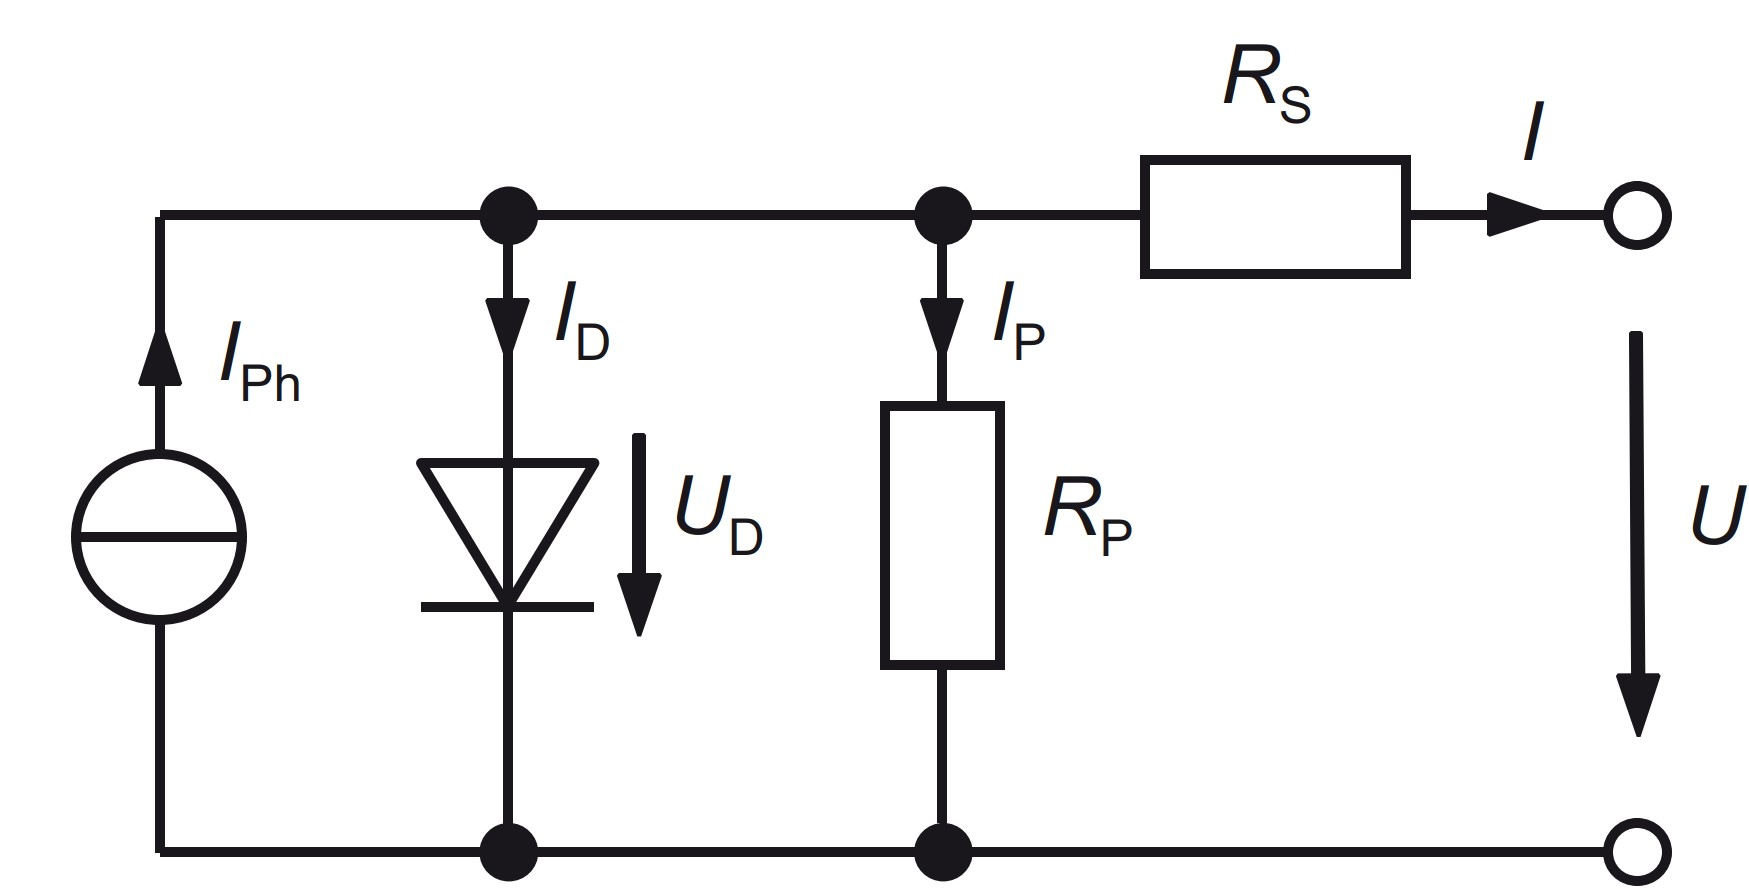
\includegraphics[width=0.98\linewidth]{images/Ersatzschaltbild_Solarzelle_2.jpg}
\end{minipage}
\hfill
\begin{minipage}[c]{0.51\columnwidth}

$
\boxed{
I = I_\text{Ph} 
- I_\text{S} \cdot \left( e^{\frac{U + I \cdot R_\text{S}}{m \cdot U_\text{T}}} - 1 \right)
- \frac{U + I \cdot R_\text{S}}{R_\text{P}}}
$

\vspace{0.1cm}

$
\boxed{I_\text{P} = \frac{U_\text{D}}{R_\text{P}} = \frac{U + I \cdot R_\text{S}}{R_\text{P}}}
$

\vspace{0.1cm}

$
\boxed{
R_\text{P} = - \left. \frac{\Delta U}{\Delta I} \right|_{U = 0}
}$
$
\boxed{
R_\text{S} = - \left. \frac{\Delta U}{\Delta I} \right|_{U = U_\text{LL}}
}
$
\end{minipage}

\vspace{0.1cm}

\begin{minipage}[t]{0.42\columnwidth}
    \renewcommand{\arraystretch}{1.2}
    \begin{tabular}{@{} l p{2.5cm} l @{}}
        $[I]$             & Solarzellenstrom \dotfill                          & $\mathrm{A}$ \\
        $[I_\text{Ph}]$   & Photostrom \dotfill                    & $\mathrm{A}$ \\
        $[I_\text{D}]$    & Diodenstrom \dotfill                                   & $\mathrm{A}$ \\
        $[I_\text{S}]$    & Sättigungsstrom \dotfill                     & $\mathrm{A}$ \\
        $[U]$             & Zellspannung \dotfill                                  & $\mathrm{V}$ \\
        $[U_\text{T}]$    & Temperaturspannung \dotfill                            & $\mathrm{V}$ \\
    \end{tabular}
\end{minipage}
\hfill
\vrule width 1pt
\hfill
\begin{minipage}[t]{0.56\columnwidth}
    \renewcommand{\arraystretch}{1.2}
    \begin{tabular}{@{} l p{3.1cm} l @{}}
        $[m]$             & Idealfaktor der Diode \dotfill & $-$ \\
        $[k]$           & Boltzmann-Konstante  \dotfill & $\mathrm{\frac{J}{K}}$ \\
        $[T]$           & Temperatur (thermodyn) \dotfill          & $\mathrm{K}$ \\
        $[q]$           & Elementarladung \dotfill & $\mathrm{C}$ \\
        $[R_\text{P}]$   & Parallelwiderstand \dotfill & $\mathrm{\Omega}$ \\
        $[R_\text{S}]$   & Serienwiderstand \dotfill & $\mathrm{\Omega}$ \\
    \end{tabular}
\end{minipage}



\columnbreak
\subsection{Spektrale Empfindlichkeit}
Die spektrale Empfindlichkeit \( S(\lambda) \) beschreibt den erzeugten Photostrom bei gegebener optischer Leistung. 



$\boxed{
S(\lambda) 
= \frac{I_{\text{Ph}}}{P_{\text{Opt}}}
}$  $\boxed{
S(\lambda) 
= \frac{\frac{Q}{\Delta t}}{\frac{W_{\text{Opt}}}{\Delta t}}
}$  $\boxed{
S(\lambda) 
= \frac{q}{h \cdot f} \cdot \eta_{\text{Ext}}
}$  $\boxed{
S(\lambda) 
= \frac{q}{h \cdot c_0} \cdot \lambda \cdot \eta_{\text{Ext}}
}$

\vspace{0.1cm}

Mit eingesetzten Konstanten ergibt sich:

\vspace{0.1cm}

$
\boxed{S(\lambda) = \frac{\lambda \cdot \eta_{\text{Ext}}}{1.24 \, \mathrm{\mu m}} \cdot \frac{\mathrm{A}}{\mathrm{W}}}
\quad
q \approx1.602 \cdot 10^{-19} \, \mathrm{Ws}
\quad
h \approx 6.6 \cdot 10^{-34} \, \mathrm{Ws^2}
\quad
c_0 \approx 3 \cdot 10^{8} \, \mathrm{\frac{m}{s}}
$

\vspace{0.1cm}

\begin{minipage}[t]{0.48\columnwidth}
    \renewcommand{\arraystretch}{1.2}
    \begin{tabular}{@{} l p{2.8cm} l @{}}
        $[S_\lambda]$       & Spektrale Empf. \dotfill          & $\frac{\mathrm{A}}{\mathrm{W}}$ \\
        $[I_\mathrm{Ph}]$   & Photostrom \dotfill               & $\mathrm{A}$ \\
        $[P_\mathrm{Opt}]$  & Optische Leist. \dotfill          & $\mathrm{W}$ \\
        $[Q]$               & Elektrische Lad. \dotfill         & $\mathrm{C}$ \\
        $[W_\mathrm{Opt}]$  & Optische Energie \dotfill         & $\mathrm{J}$ \\
        $[q]$               & Elementarladung \dotfill          & $\mathrm{C}$ 
    \end{tabular}
\end{minipage}
\hfill
\vrule width 1pt
\hfill
\begin{minipage}[t]{0.48\columnwidth}
    \renewcommand{\arraystretch}{1.2}
    \begin{tabular}{@{} l p{2.8cm} l @{}}
        $[h]$                 & Planck-Konstante \dotfill         & $\mathrm{J \cdot s}$ \\
        $[f]$                 & Frequenz \dotfill                 & $\mathrm{Hz}$ \\
        $[\eta_\mathrm{Ext}]$ & Externe Quanteneff. \dotfill      & $-$ \\
        $[c_0]$               & Lichtgeschwindigkeit \dotfill     & $\frac{\mathrm{m}}{\mathrm{s}}$\\
        $[\lambda]$           & Wellenlänge \dotfill              & $\mathrm{m}$
    \end{tabular}
\end{minipage}



\subsection{Füllfaktor und Wirkungsgrad von Solarzellen}

$
\boxed{
FF = \frac{U_{\text{MPP}} \cdot I_{\text{MPP}}}{U_{\text{L}} \cdot I_{\text{K}}} 
}$
$
\boxed{
FF = \frac{P_{\text{MPP}}}{U_{\text{L}} \cdot I_{\text{K}}}
}$
$
\boxed{
\eta = \frac{P_{\text{MPP}}}{P_{\text{opt}}} 
}$
$
\boxed{
P_{\text{MPP}} = FF \cdot U_{\mathrm{L}} \cdot I_{\mathrm{K}}
}$
$
\boxed{
P_{\text{opt}} = E \cdot A
}
$

\vspace{0.1cm}

\begin{minipage}[t]{0.44\columnwidth}
    \renewcommand{\arraystretch}{1.2}
    \begin{tabular}{@{} l p{2.4cm} l @{}}
        $[FF]$               & Füllfaktor \dotfill                            & $-$ \\
        $[\eta]$             & Wirkungsgrad \dotfill                          & $-$ \\
        $[U_{\text{MPP}}]$   & MPP-Spannung \dotfill      & $\mathrm{V}$ \\
        $[I_{\text{MPP}}]$   & MPP-Strom \dotfill         & $\mathrm{A}$ \\
        $[P_{\text{MPP}}]$   & MPP-Leistung \dotfill      & $\mathrm{W}$ \\
    \end{tabular}
\end{minipage}
\hfill
\vrule width 1pt
\hfill
\begin{minipage}[t]{0.52\columnwidth}
    \renewcommand{\arraystretch}{1.2}
    \begin{tabular}{@{} l p{3cm} l @{}}
        $[U_{\text{L}}]$     & Leerlaufspannung \dotfill                      & $\mathrm{V}$ \\
        $[I_{\text{K}}]$     & Kurzschlussstrom \dotfill                      & $\mathrm{A}$ \\
        $[E]$                & Einstrahlung \dotfill                          & $\mathrm{\frac{W}{m^2}}$ \\
        $[A]$                & Zellenfläche \dotfill                          & $\mathrm{m^2}$ \\
        $[P_{\text{opt}}]$   & Einstrahlleistung $= E \cdot A$ \dotfill & $\mathrm{W}$ \\
    \end{tabular}
\end{minipage}



\subsection{Verlustmechan. durch unpassende Energie der Photonen}

Eine fundamentale Begrenzung des Wirkungsgrads von Solarzellen ergibt sich aus dem materialabhängigen Bandabstand $\Delta W_G$ des Halbleiters. Die Wellenlänge, bei der Licht gerade noch absorbiert wird, nennen wir die \textbf{Bandlückenwellenlänge} $\lambda_G$ mit

$\boxed{\lambda_{\mathrm{G}} = \frac{h \cdot c_0}{\Delta W_G}}$
$\boxed{\Delta W_{\mathrm{G\_Krist.\ Silizium}} = 1.12e\mathrm{V}}$

\vspace{0.1cm}

\renewcommand{\arraystretch}{1.2} % Erhöht Zeilenhöhe für bessere Lesbarkeit
\begin{tabular}{@{} l p{6cm} l @{}}
    
    
\end{tabular}

\begin{minipage}[t]{0.5\columnwidth}
    \renewcommand{\arraystretch}{1.2}
    \begin{tabular}{@{} l p{3.2cm} l @{}}
        $[\lambda_{\mathrm{G}}]$       & Grenzwellenlänge Bandl    \dotfill & $\mathrm{m}$ \\
        $[h]$               & Planck-Konstante          \dotfill & $\mathrm{J \cdot s}$ \\
        $[c_0]$             & Lichtgeschwindigkeit      \dotfill & $\frac{\mathrm{m}}{\mathrm{s}}$ \\
    \end{tabular}
\end{minipage}
\hfill
\vrule width 1pt
\hfill
\begin{minipage}[t]{0.45\columnwidth}
    \renewcommand{\arraystretch}{1.2}
    \begin{tabular}{@{} l p{2.4cm} l @{}}
        $[W_{\mathrm{G}}]$             & Energie Photon            \dotfill & $\mathrm{J}$ \\
        $[\Delta W_{\mathrm{G}}]$      & Bandlücke   \dotfill & $\mathrm{J}$ \\
    \end{tabular}
\end{minipage}

\vspace{0.1cm}

\begin{minipage}[t]{0.48\columnwidth}
    \myul{\textbf{$\lambda > \lambda_G$ : Durchstrahlung}}\\
    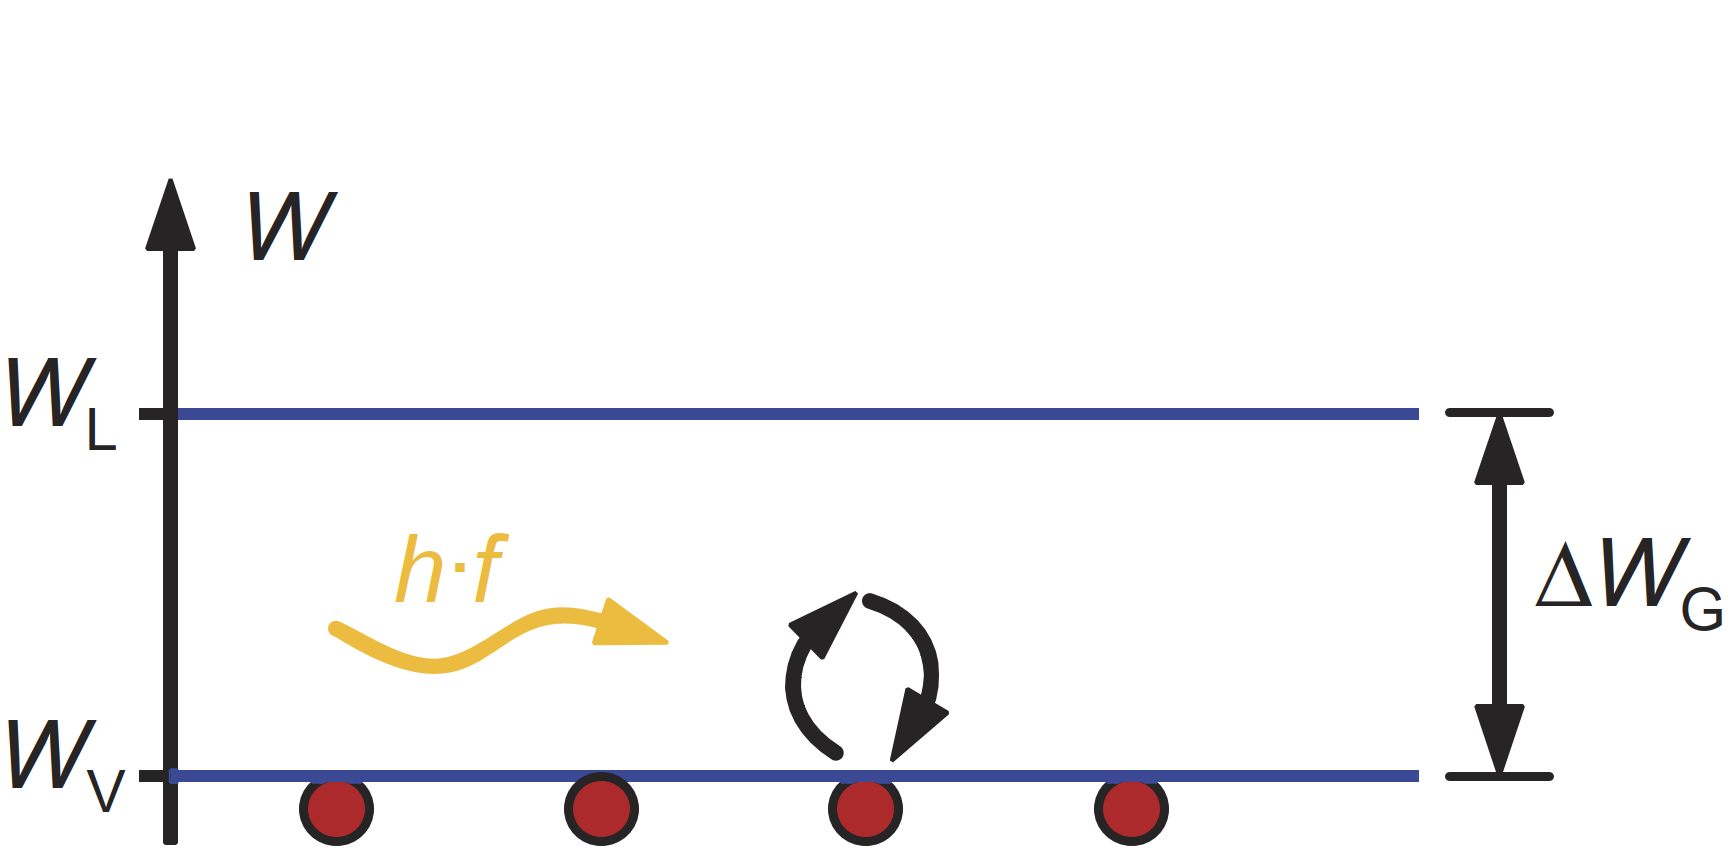
\includegraphics[width=0.9\columnwidth]{images/Spektraler_Wirkungsgrad_Durchstrahlung.png}
\end{minipage}
\hfill
\begin{minipage}[t]{0.48\columnwidth}
    \myul{\textbf{$\lambda < \lambda_G$ : Thermalisierung}}\\
    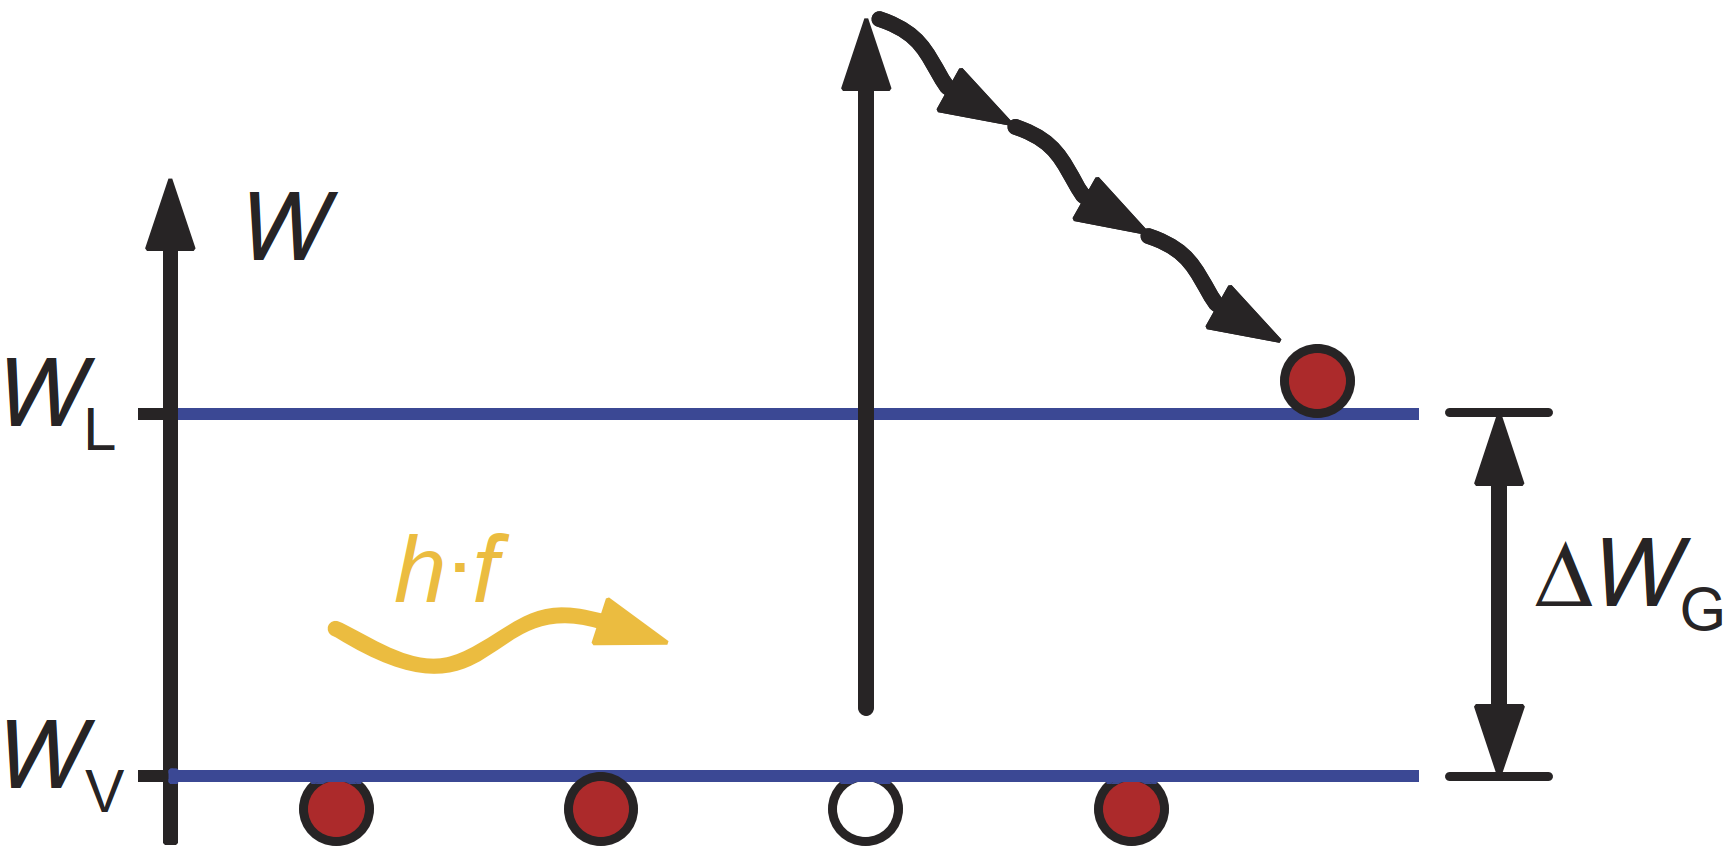
\includegraphics[width=0.9\columnwidth]{images/Spektraler_Wirkungsgrad_Thermalisierung.png}
\end{minipage}

\vspace{0.1cm}

\myul{\textbf{Durchstrahlung}} bezeichnet den Verlustmechanismus, bei dem Photonen mit zu geringer Energie die Solarzelle durchqueren, ohne absorbiert zu werden.\\
\myul{\textbf{Thermalisierung}} beschreibt den Energieverlust, bei dem Photonen mit zu hoher Energie nur einen Teil ihrer Energie an Elektronen abgeben, während die überschüssige Energie als Wärme verloren geht.



\subsection{Spektraler Wirkungsgrad $\eta_\text{S}$}

Der spektrale Wirkungsgrad gibt an, welcher Teil der einfallenden Strahlungsleistung theoretisch mit einem Halbleiter des Bandabstands \( \Delta W_G \) genutzt werden kann. Die Transmissionsverluste beschreiben den Teil des Spektrums, dessen Photonen zu energiearm sind, um die Bandlücke zu überwinden. Thermalisierungsverluste treten dagegen bei Photonen auf, die energiereicher sind als die Bandlücke. In diesem Fall kann nur ein Teil der Energie für den Halbleiter genutzt werden, der Rest wird in Wärme umgewandelt.


\vspace{0.1cm}

$
\boxed{
\eta_\text{S} = \frac{P_\text{El}}{P_\text{Opt}} = \frac{U_\text{Max} \cdot j_\text{Max}}{E}
}$
$
\boxed{
P_\text{El} = U_\text{Max} \cdot I_\text{Max} = U_\text{Max} \cdot j_\text{Max} \cdot A
}$
$
\boxed{
U_\text{Max} = \frac{\Delta W_\text{G}}{q}
}
$

\vspace{0.1cm}

\begin{minipage}[t]{0.48\columnwidth}
    \renewcommand{\arraystretch}{1.2}
    \begin{tabular}{@{} l p{2.7cm} l @{}}
        $[U_\text{Max}]$  & Maximale Spannung \dotfill        & $\mathrm{V}$ \\
        $[\Delta W_\text{G}]$  & Bandlücke \dotfill           & $\mathrm{eV}$ \\
        $[q]$             & Elementarladung \dotfill          & $\mathrm{C}$ \\
        $[P_\text{El}]$   & Elektrische Leistung \dotfill     & $\mathrm{W}$ \\
        $[I_\text{Max}]$  & Maximalstrom \dotfill             & $\mathrm{A}$ \\
    \end{tabular}
\end{minipage}
\hfill
\vrule width 1pt
\hfill
\begin{minipage}[t]{0.48\columnwidth}
    \renewcommand{\arraystretch}{1.2}
    \begin{tabular}{@{} l p{2.7cm} l @{}}
        $[j_\text{Max}]$  & Stromdichte \dotfill              & $\mathrm{A/m^2}$ \\
        $[A]$             & Zellenfläche \dotfill             & $\mathrm{m^2}$ \\
        $[P_\text{Opt}]$  & Eingestr Leistung \dotfill & $\mathrm{W}$ \\
        $[E]$             & Bestrahlungsstärke \dotfill       & $\mathrm{W/m^2}$ \\
        $[\eta_\text{S}]$ & Spektr Wirkungsgrad \dotfill  & $\mathrm{-}$ \\
    \end{tabular}
\end{minipage}



\subsection{Spektrale Verluste}
%\begin{center}
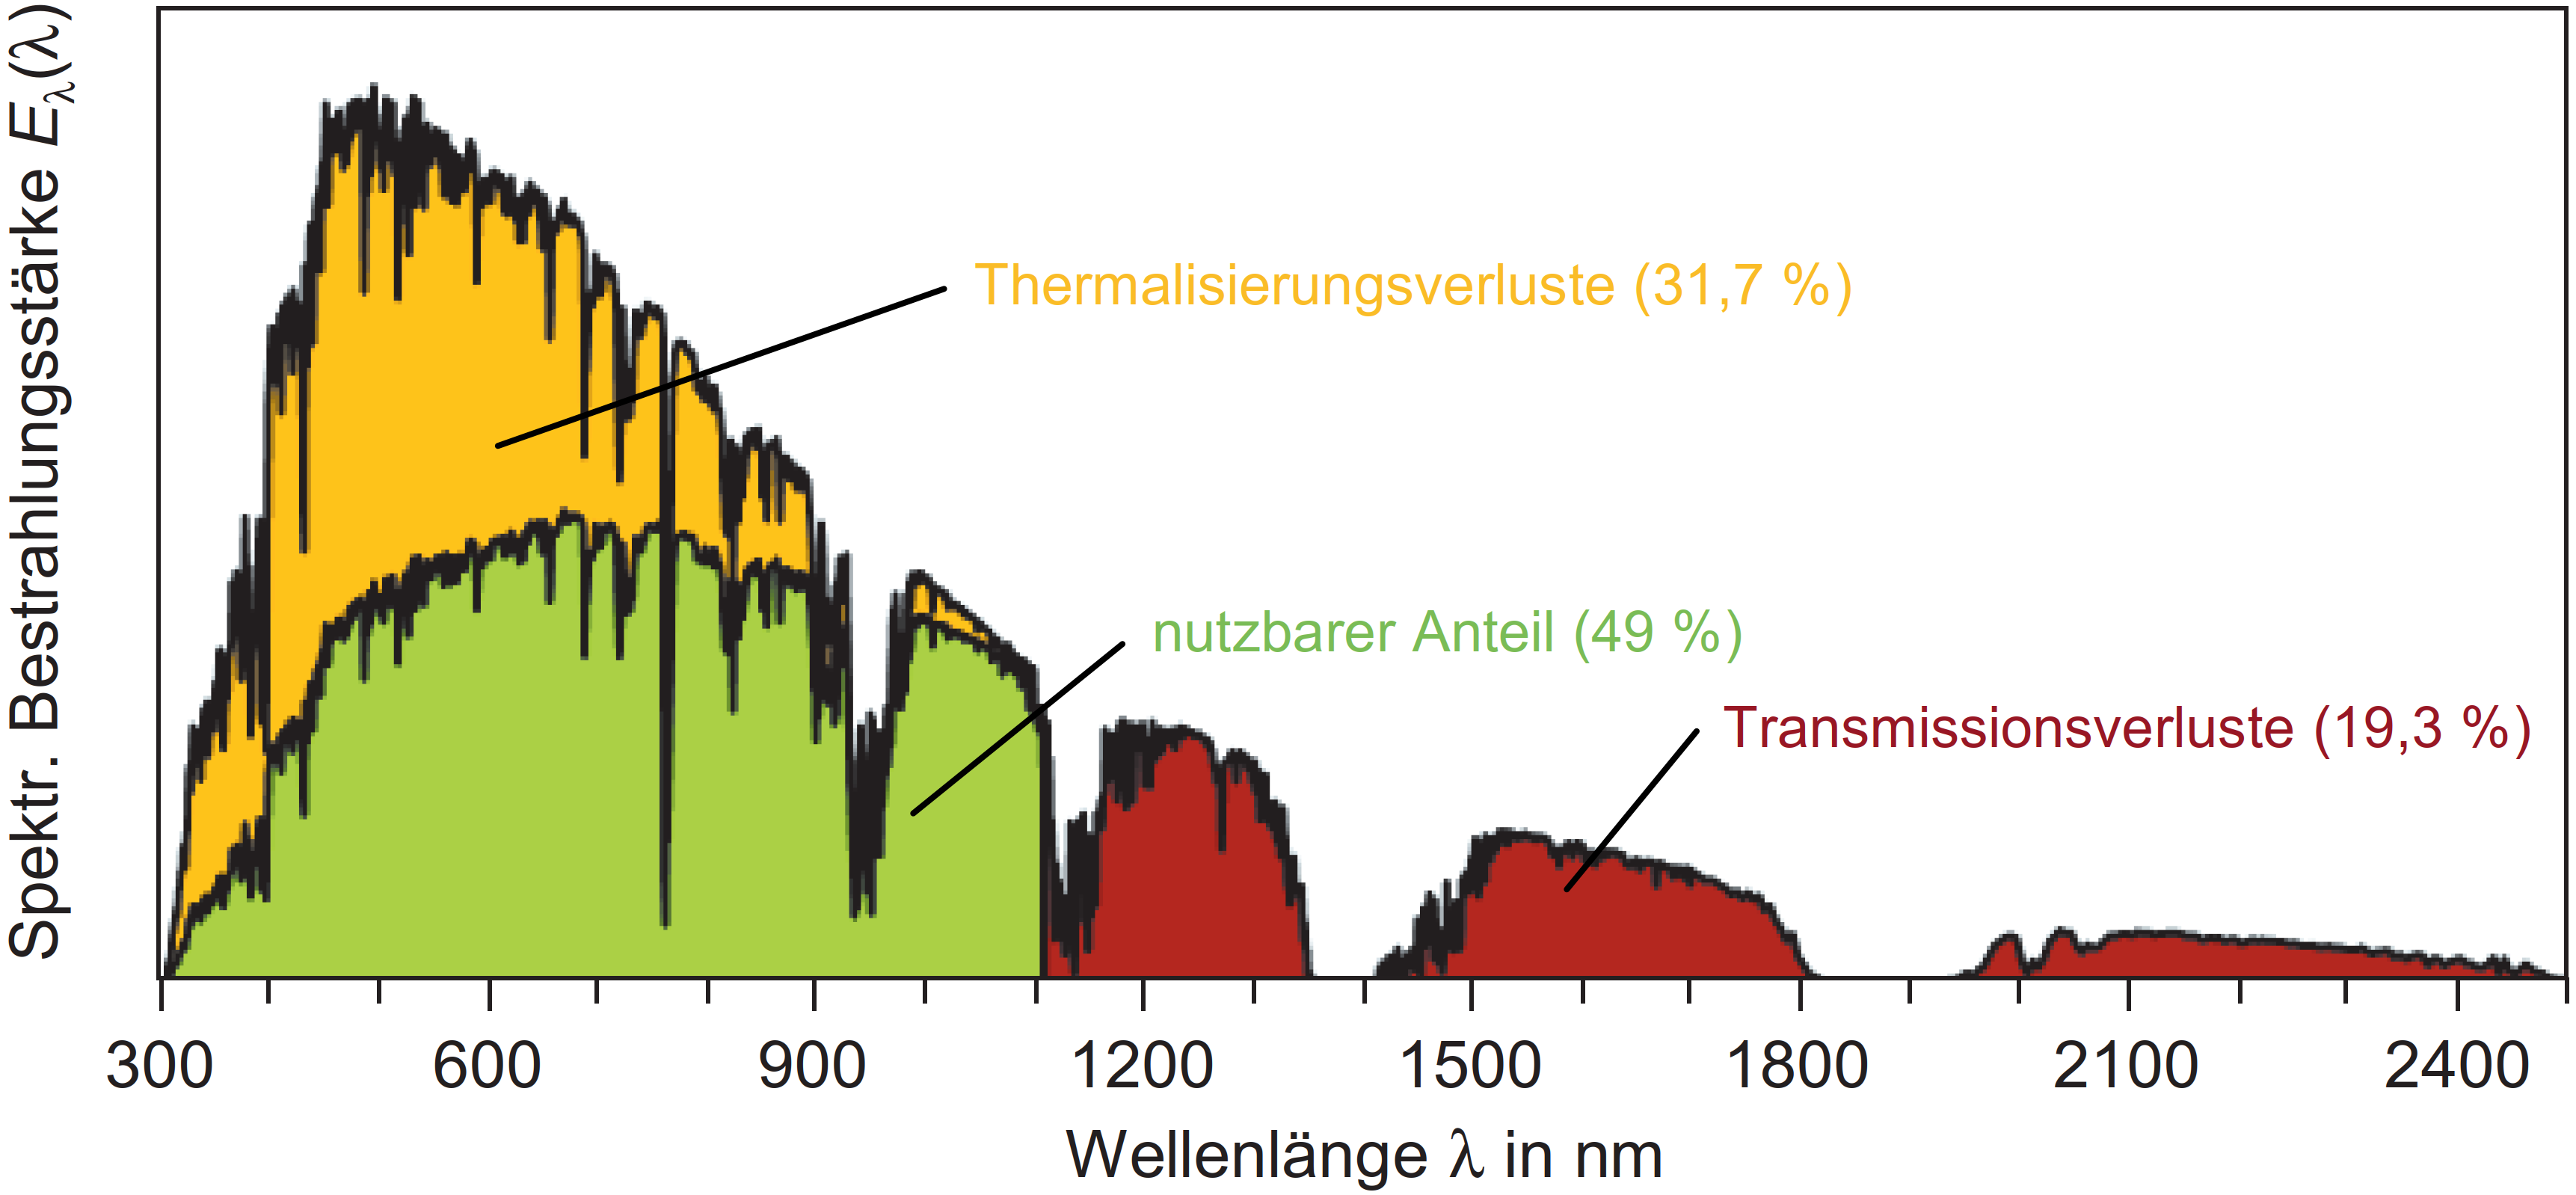
\includegraphics[width=0.8\columnwidth]{images/Spektrale_Verluste.png}
%\end{center}


\subsection{Spektrale Wirkungsgrad idealer Solarzelle}
%\textbf{Theor. max mögliche Wirkungsgr} für kristalline Siliziumsolarzelle liegt bei
%ca. $29\%$. Aktuell: $\eta_{max}$ Zelle: $27.6\%$, $\eta_{max}$ Modul: $25.4\%$, $\eta$ Typisch Module: $21-23\%$

\begin{itemize}
  \item Theoretisch maximaler Wirkungsgrad: ca. 29\,\%
  \item Aktuell erreichter maximaler Wirkungsgrad von Solarzellen: 27.6\,\%
  \item Aktuell erreichter maximaler Wirkungsgrad von Solarmodulen: 25.4\,\%
  \item Typischer Wirkungsgrad aktueller Module: ca. 21--23\,\%
\end{itemize}

%\begin{center}
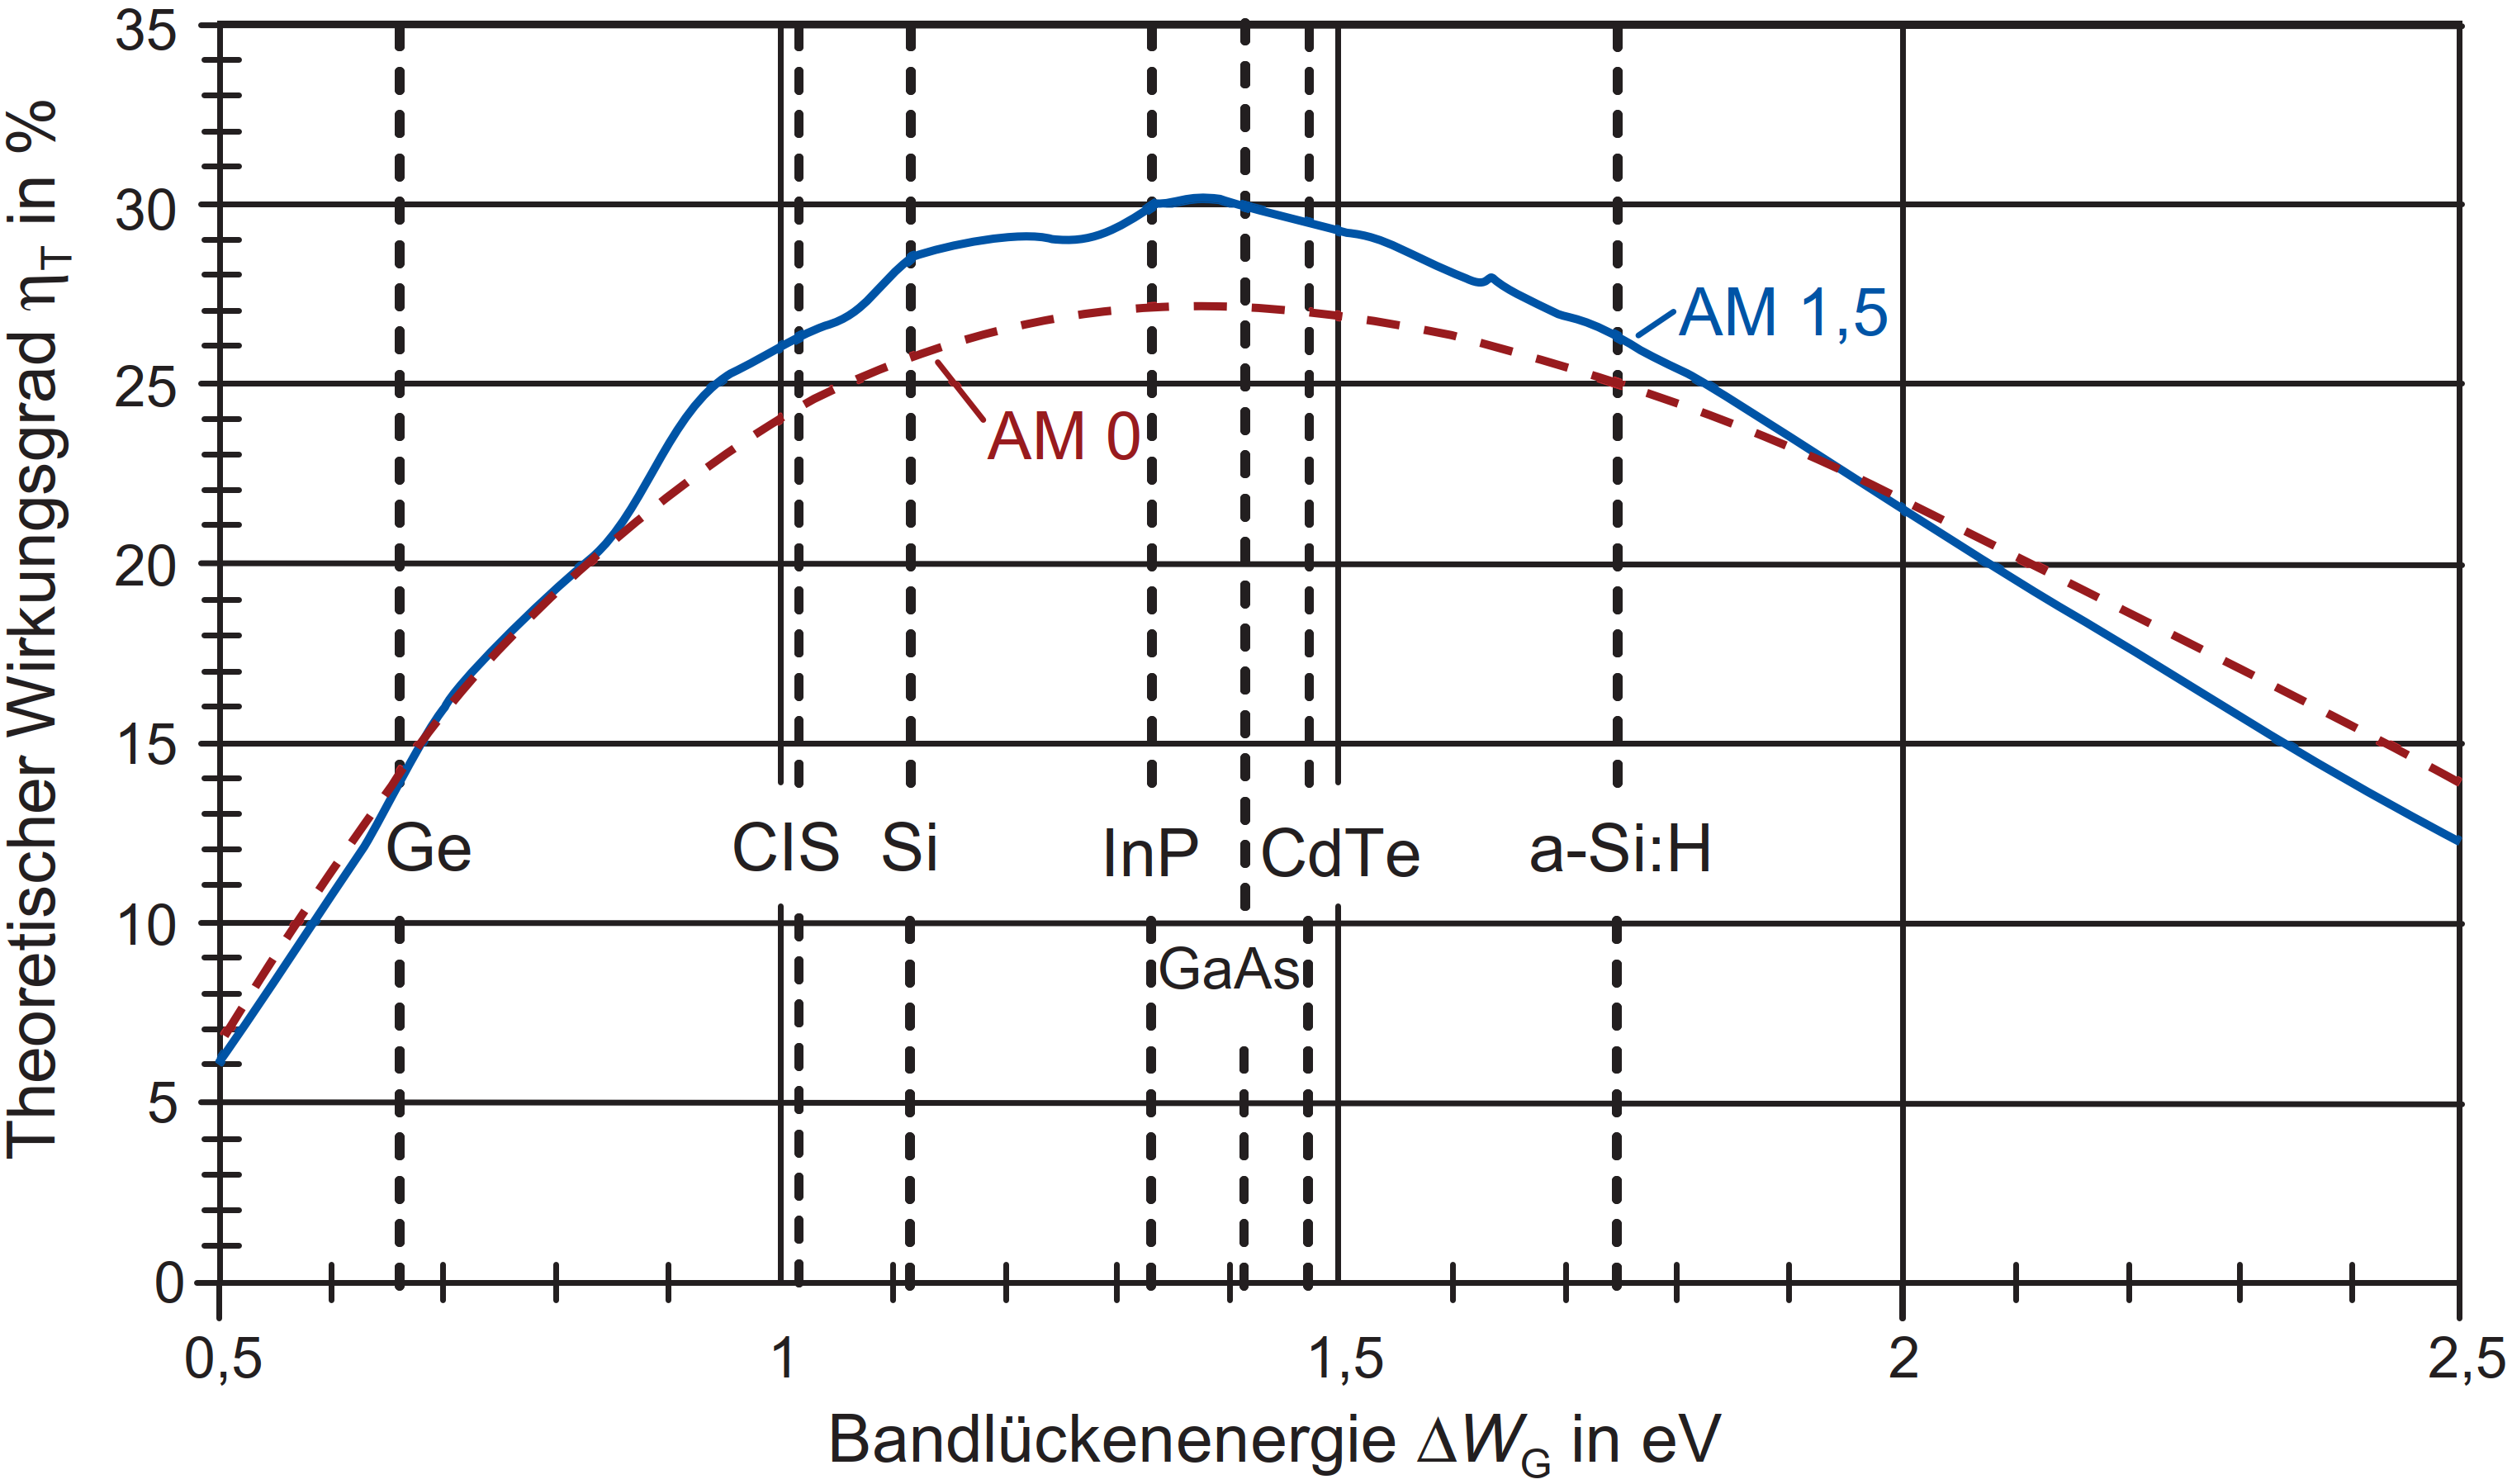
\includegraphics[width=0.8\columnwidth]{images/Spektraler_Wirkungsgrad_idealer_Solarzelle.png}
%\end{center}

\subsection{Produktionsschritte}
Für die Herstellung eines monokristallinen Solarmoduls ausgehend von Quarzsand:

\vspace{0.1cm}

\begin{enumerate}
    \item Herstellung von hochreinem Silizium (Solar-Grade-Silizium)
    \item Herstellung von monokristallinem Silizium (Ingots) im Czochralski-Verfahren
    \item Waferherstellung
    \item Solarzellenherstellung
    \item Solarmodulherstellung
\end{enumerate}

\subsection{Mehrfach- Stapelzellen}
Sie sind aus verschiedenen Halbleitermaterialien mit vers. Bandlücken aufgebaut. Es werden Photon unterschiedlicher Wellenlänge absorbiert. Damit werden höhere Wirkungsgrade erreicht (aktuell bis zu 40\%).

\subsection{Verlustfaktoren von Solarzellen: Minimierungen}

\begin{itemize}
  \item \textbf{Abschattung}: Minimierung von Kontaktfinger- und Busbarfläche, Einsatz vieler dünner Busbars, Rückseitenkontaktierung (z.B. IBC-Zelle)
  \item \textbf{Reflexion}: Antireflexbeschichtung, Texturierung der Zelloberfläche (z.B. Pyramidenstruktur)
  \item \textbf{Störstellenrekombination}: Verwendung von hochreinem Silizium (Solar-Grade), Einsatz von n-Typ Zellen
  \item \textbf{Oberflächenrekombination}: Passivierung der Oberfläche, punktuelle Kontaktierung, Durchtunnelungsschicht, Back-Surface-Field (BSF)
  \item \textbf{Transmission}: Reflektionsschicht (Oxidschicht) auf der Zellrückseite
  \item \textbf{Metall-Halbleiter-Übergang}: Lokale dotierte Schichten ($\mathrm{n^+}$ bei p-Typ, $\mathrm{p^+}$ bei n-Typ Zellen)
\end{itemize}




        \section{Einsatz von Bypassdioden}

\subsection{Gründe für Einsatz von Bypassdioden}
\begin{enumerate}
    \item Vermeidung von Überhitzung verschatteter Zellen (Hotspots)
    \item Leistungssteigerung indem sichergestellt wird, dass bei Verschattung eines Moduls nicht der gesamte String beeinträchtigt wird. (Modul bzw. Zelle wird "übersprungen")
\end{enumerate}



\subsection{Solarmodul ohne Bypassdioden}
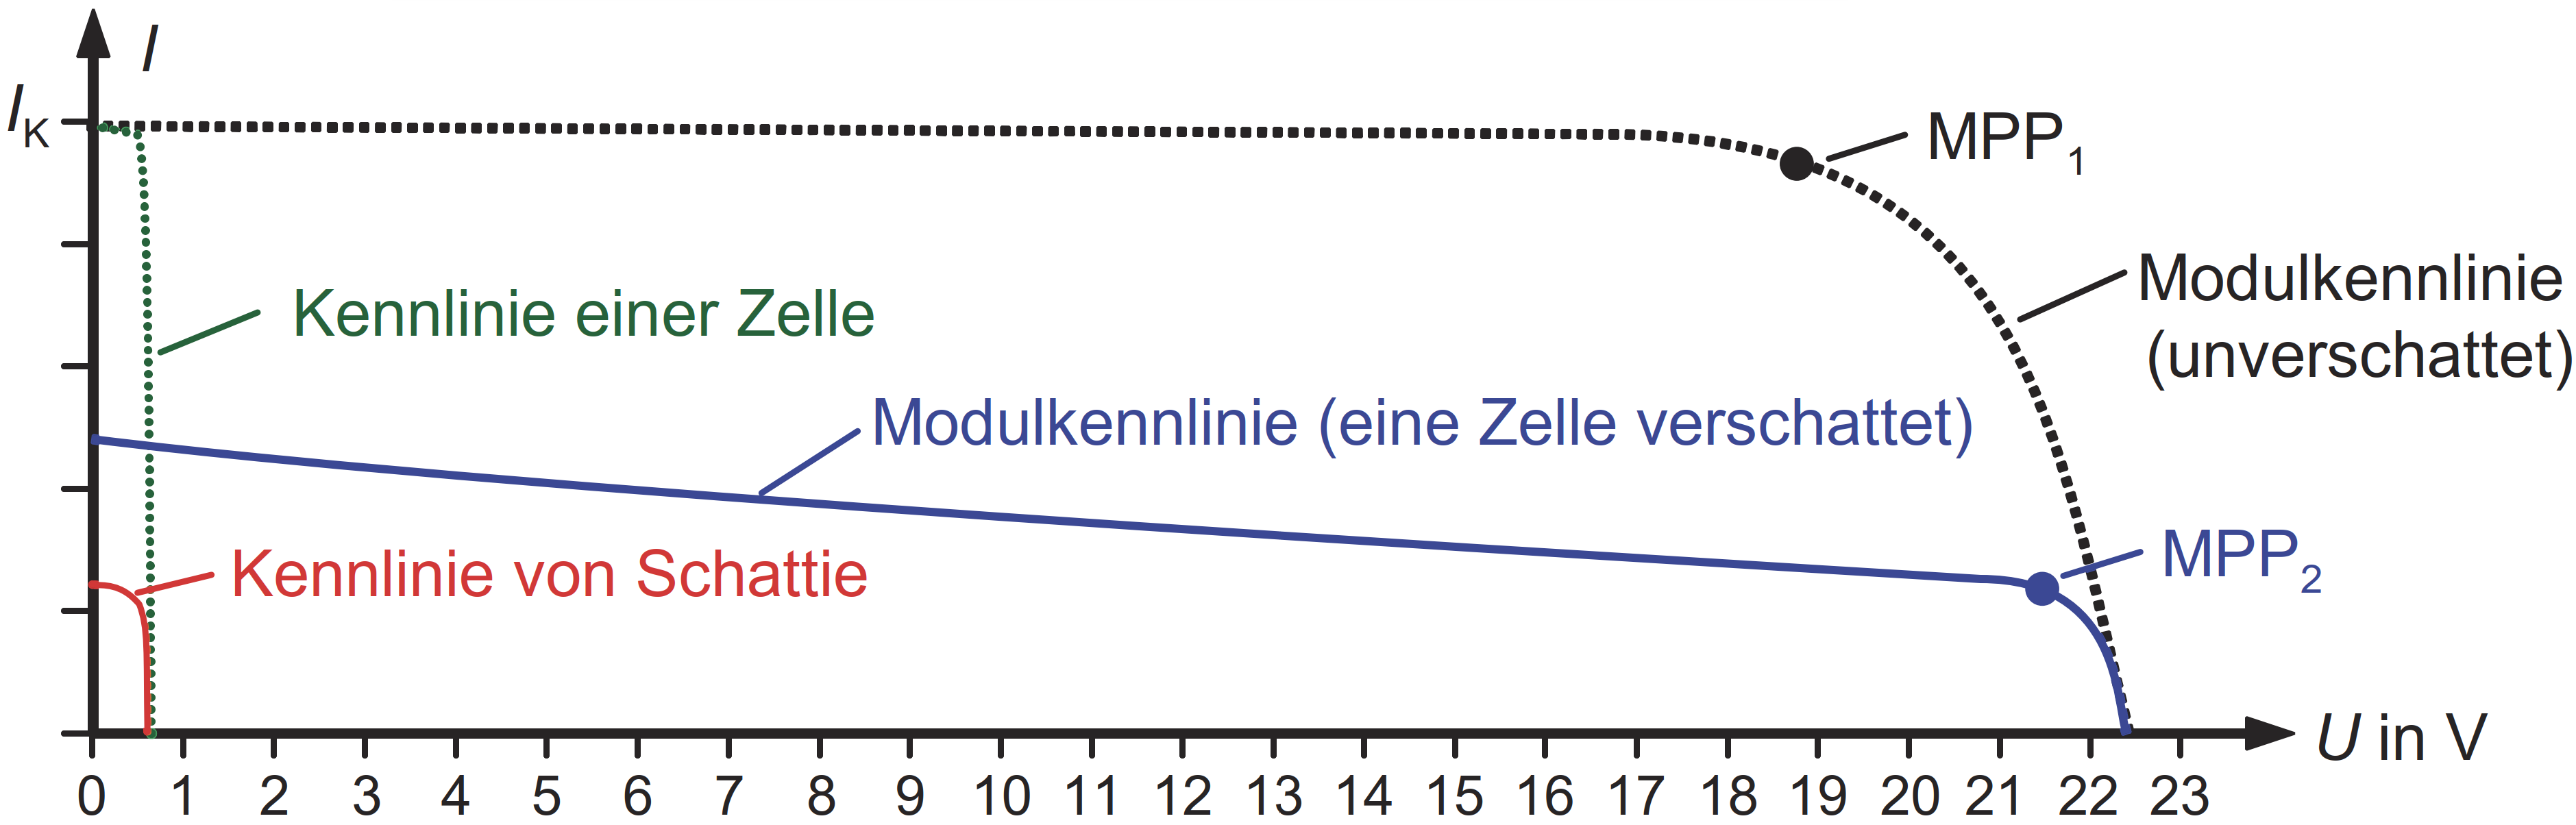
\includegraphics[width=0.95\columnwidth]{images/Verschattungsverluste_ohne_Bypassdiode.png}



\subsection{Solarmodul mit Bypassdioden}
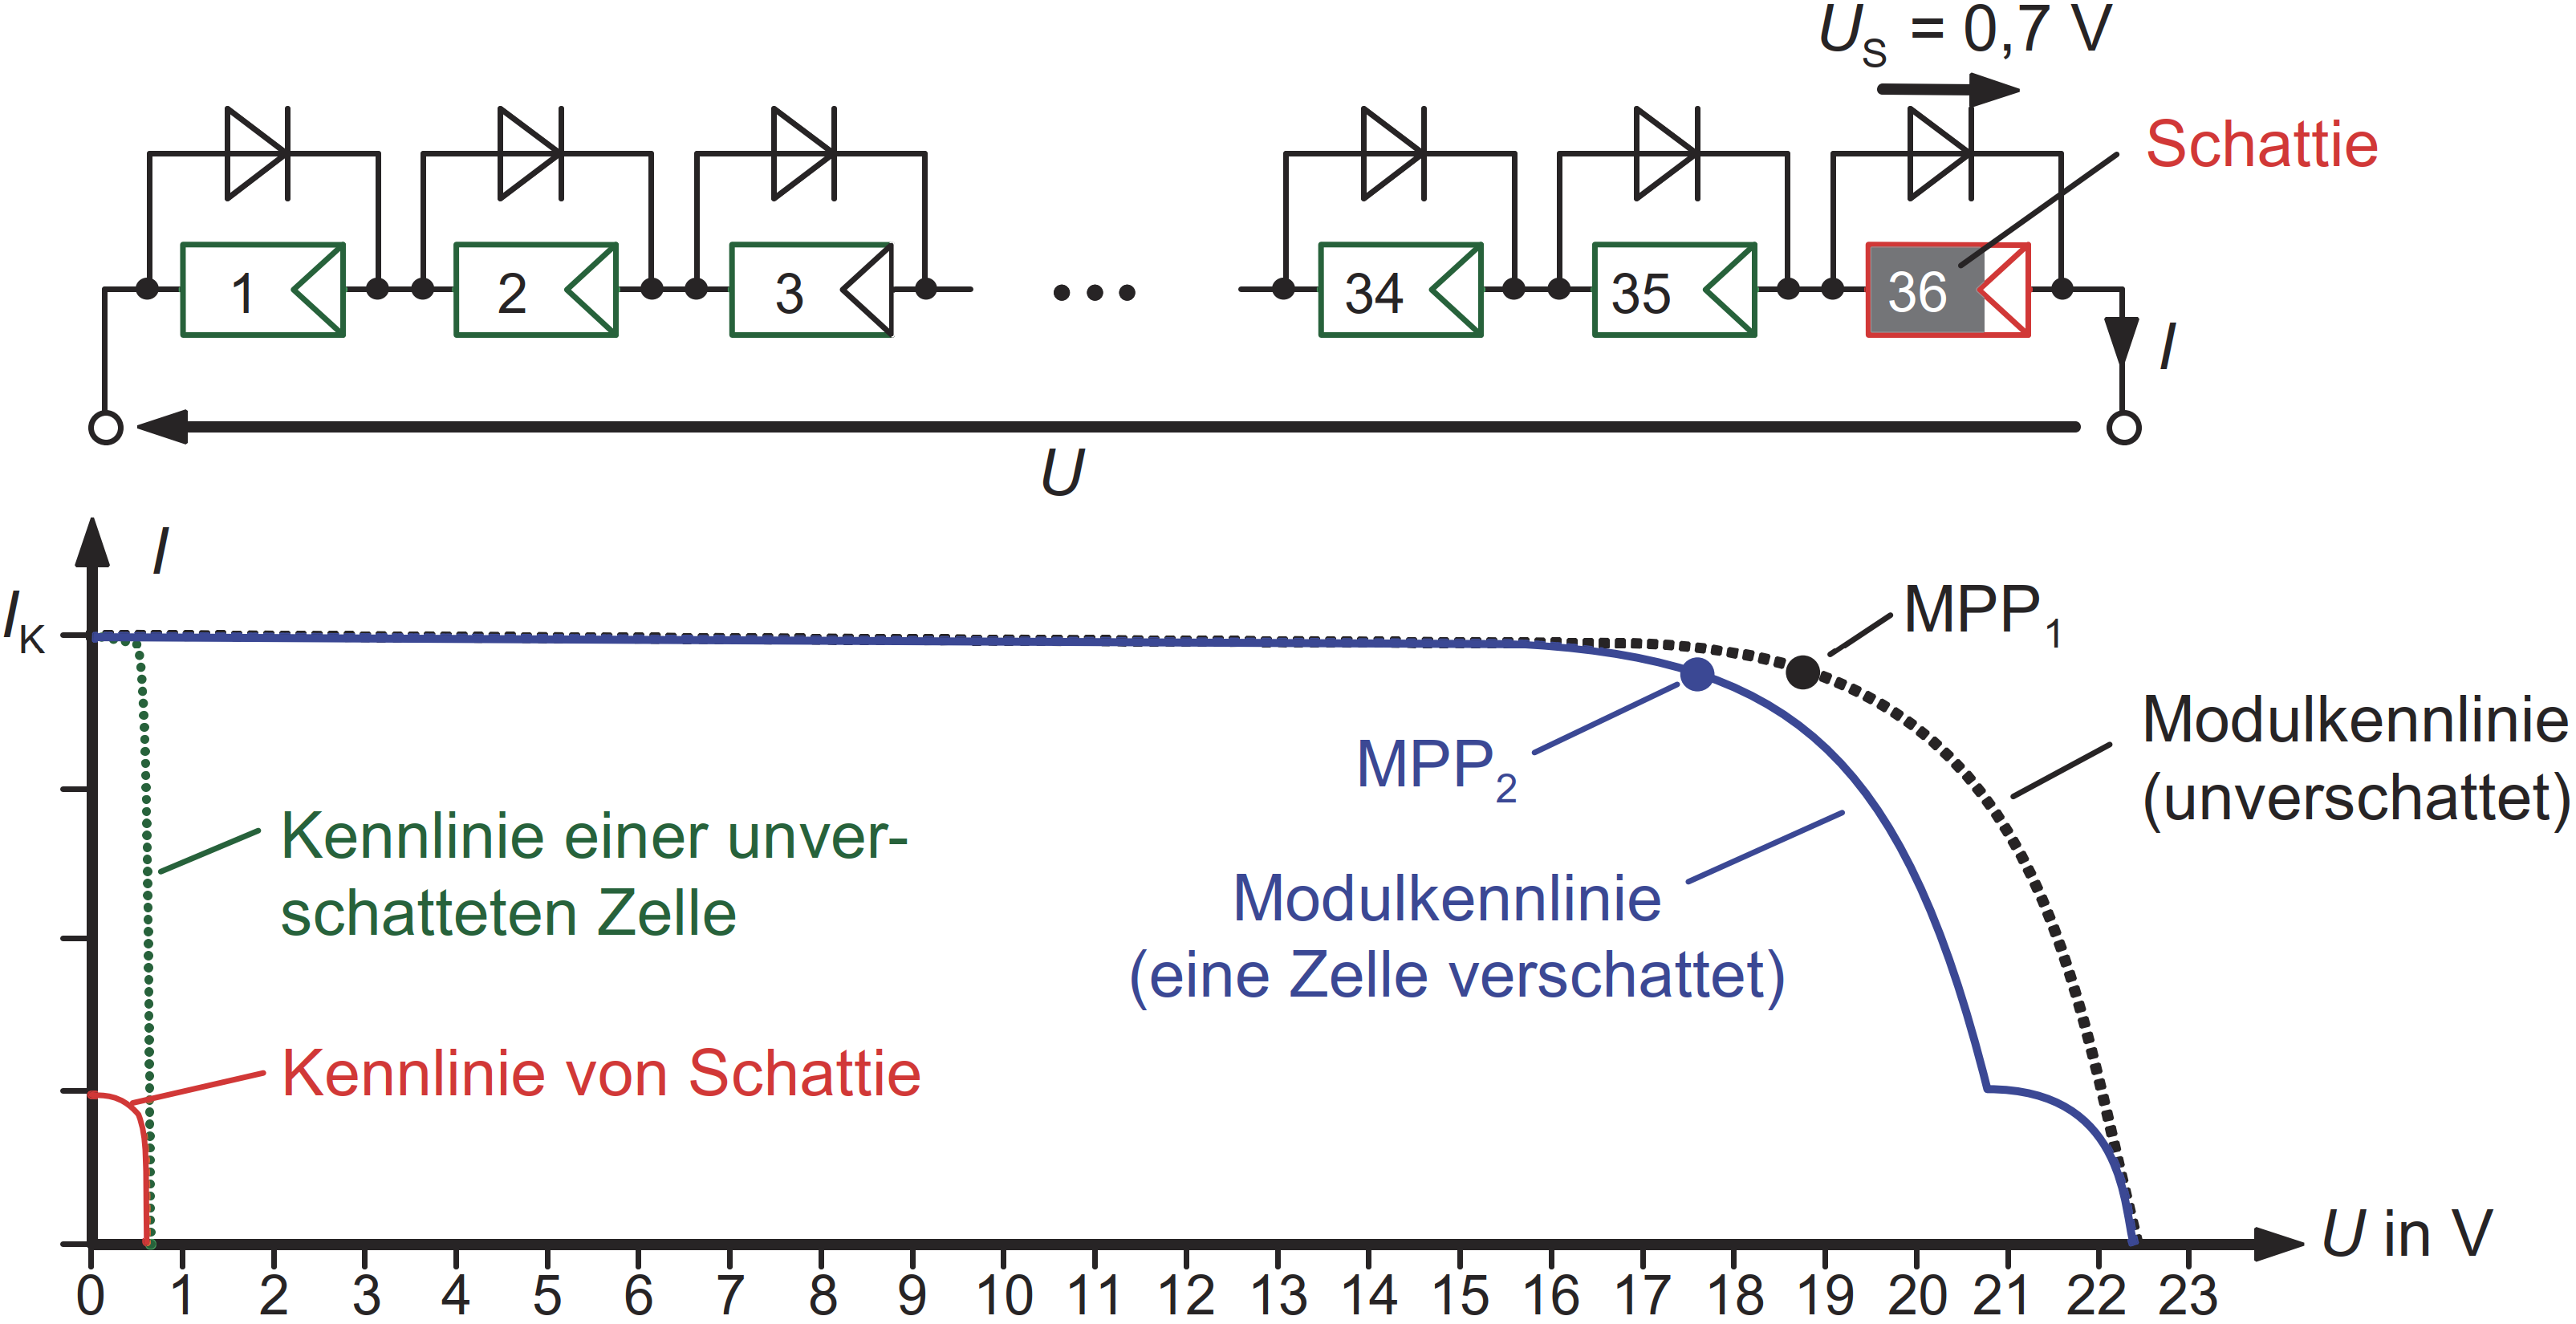
\includegraphics[width=0.95\columnwidth]{images/Verschattungsverluste_mit_Bypassdiode.png}



\subsection{Auswirkung Anzahl Bypassdioden}
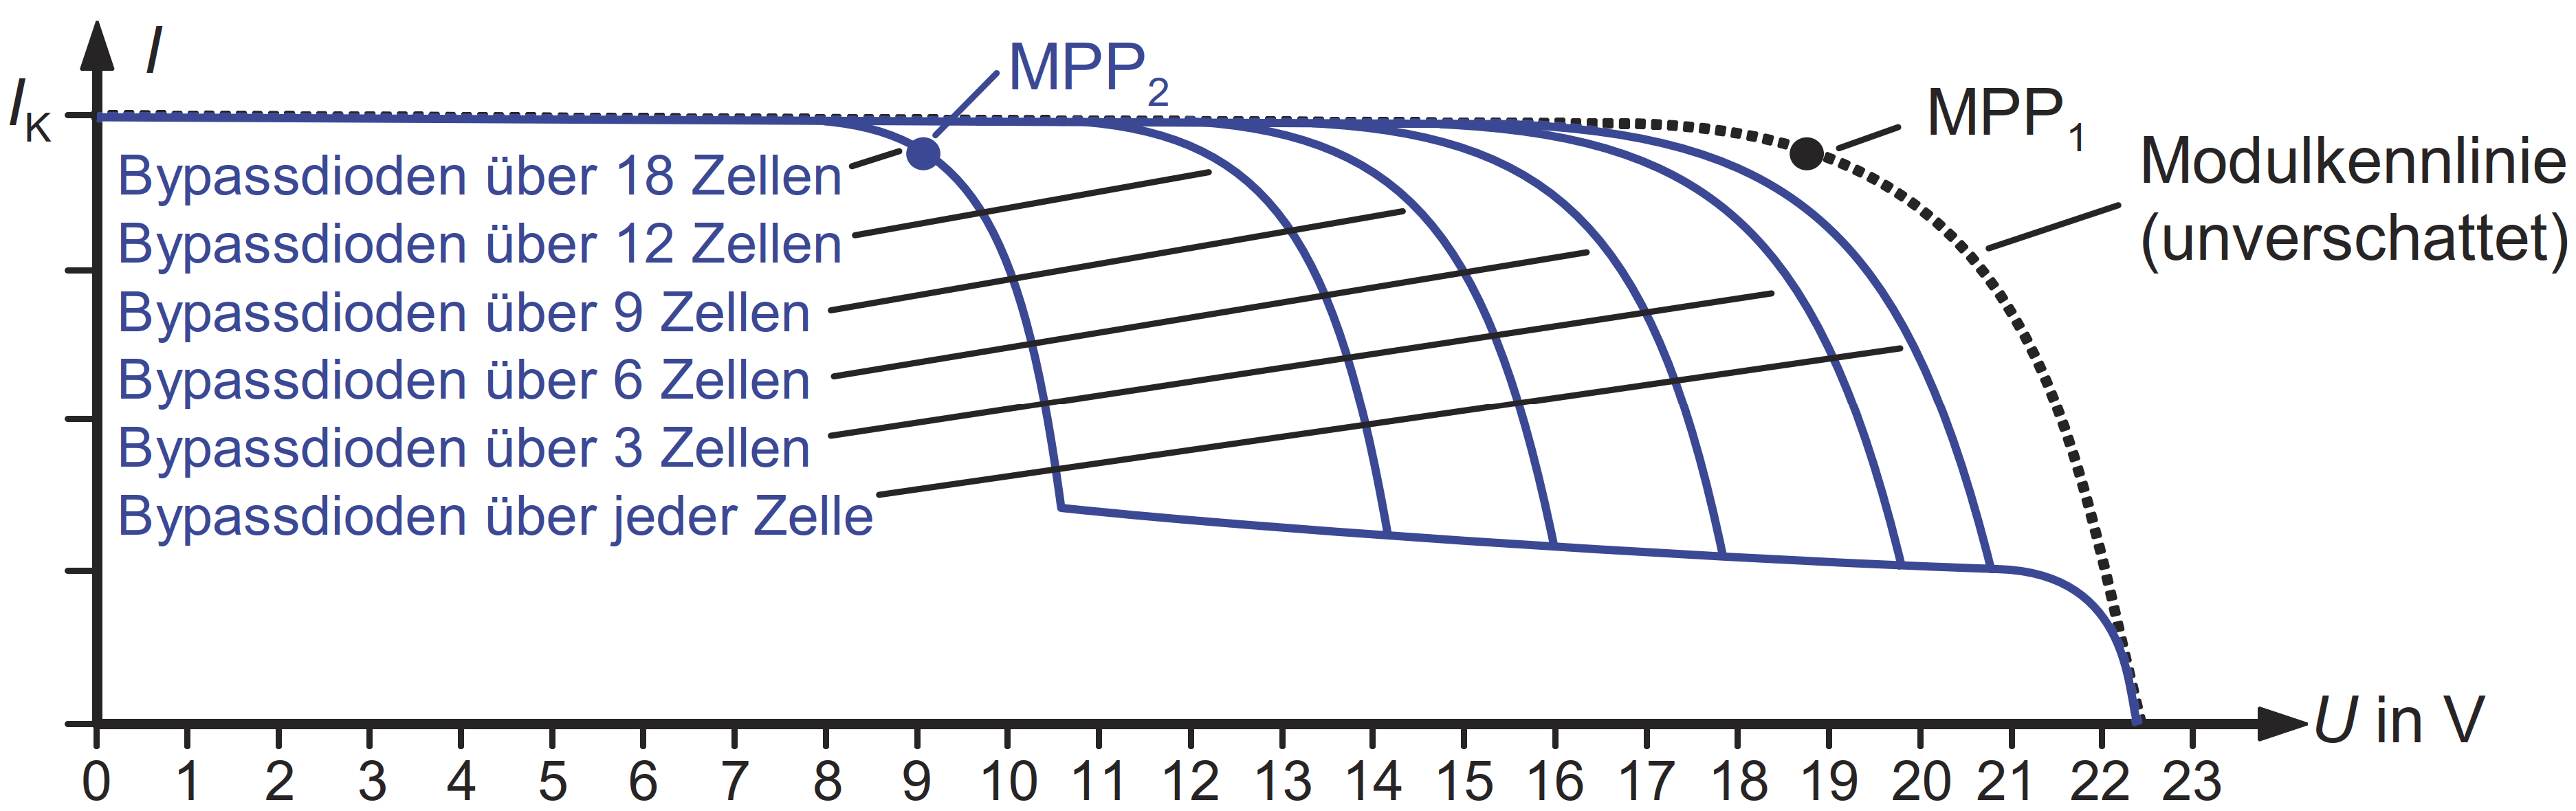
\includegraphics[width=0.95\columnwidth]{images/Reduzierung_Verschattungsverluste_durch_Bypassdioden.png}


\subsection{Vermeidung von Hotspots durch Bypassdioden}
\subsubsection{Solarmodul ohne Bypassdioden}
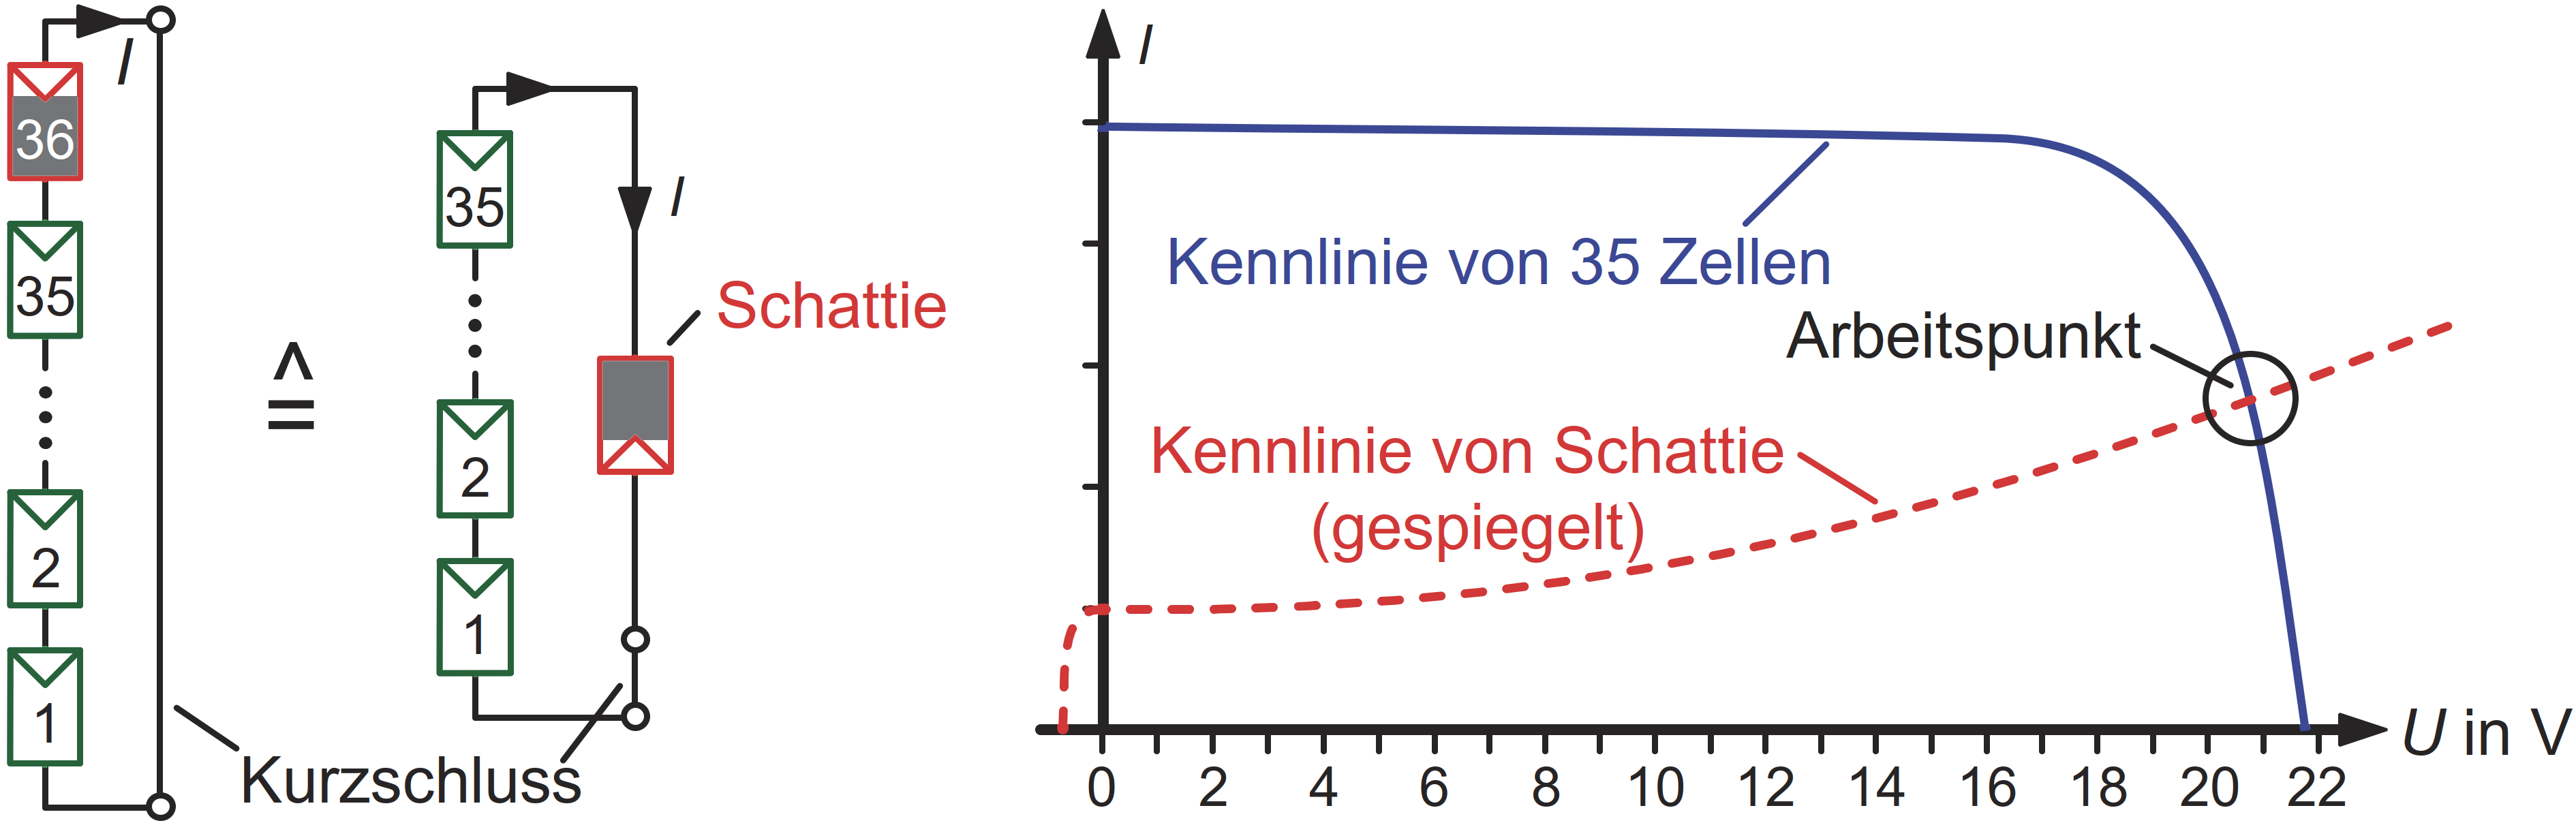
\includegraphics[width=0.95\columnwidth]{images/Vermeidung_von_Hotspots_1.png}



\subsubsection{Solarmodul mit 2 Bypassdioden}
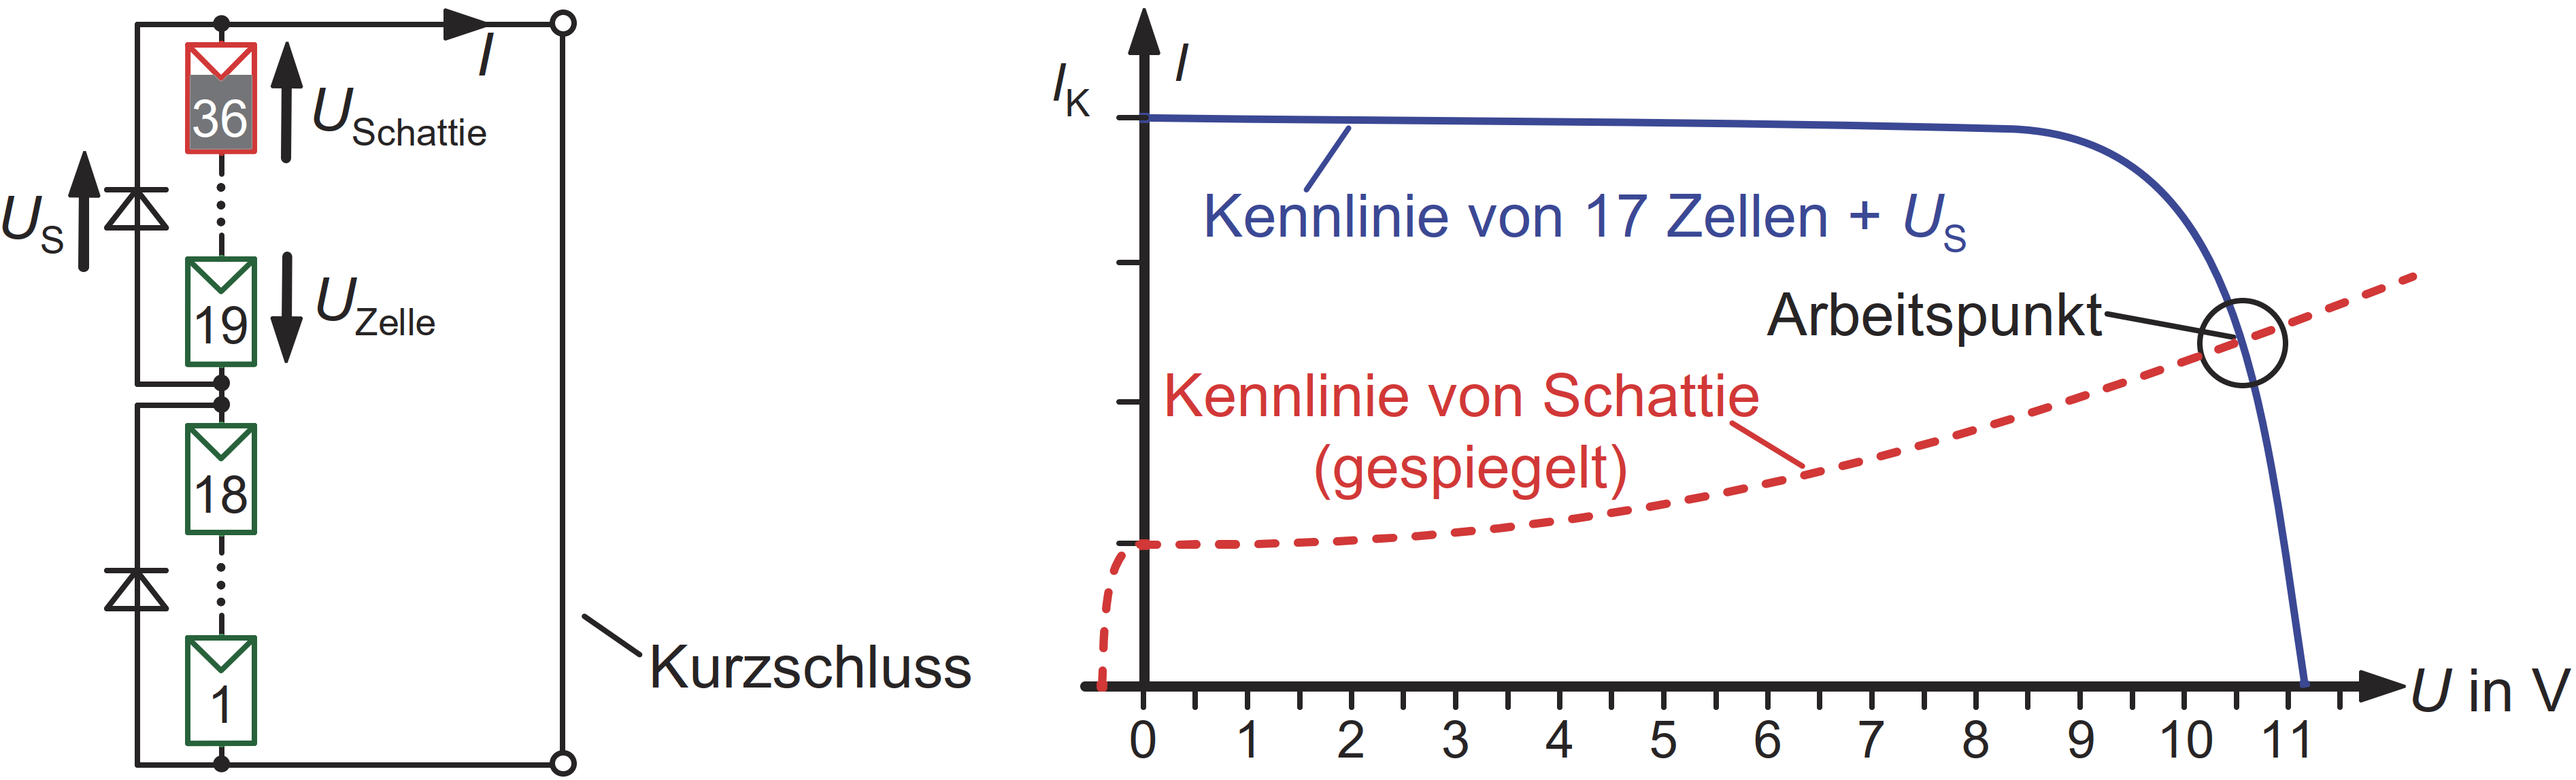
\includegraphics[width=0.95\columnwidth]{images/Vermeidung_von_Hotspots_2.png}



\subsubsection{Betrachtung verschiedener Verschattungsgrade}
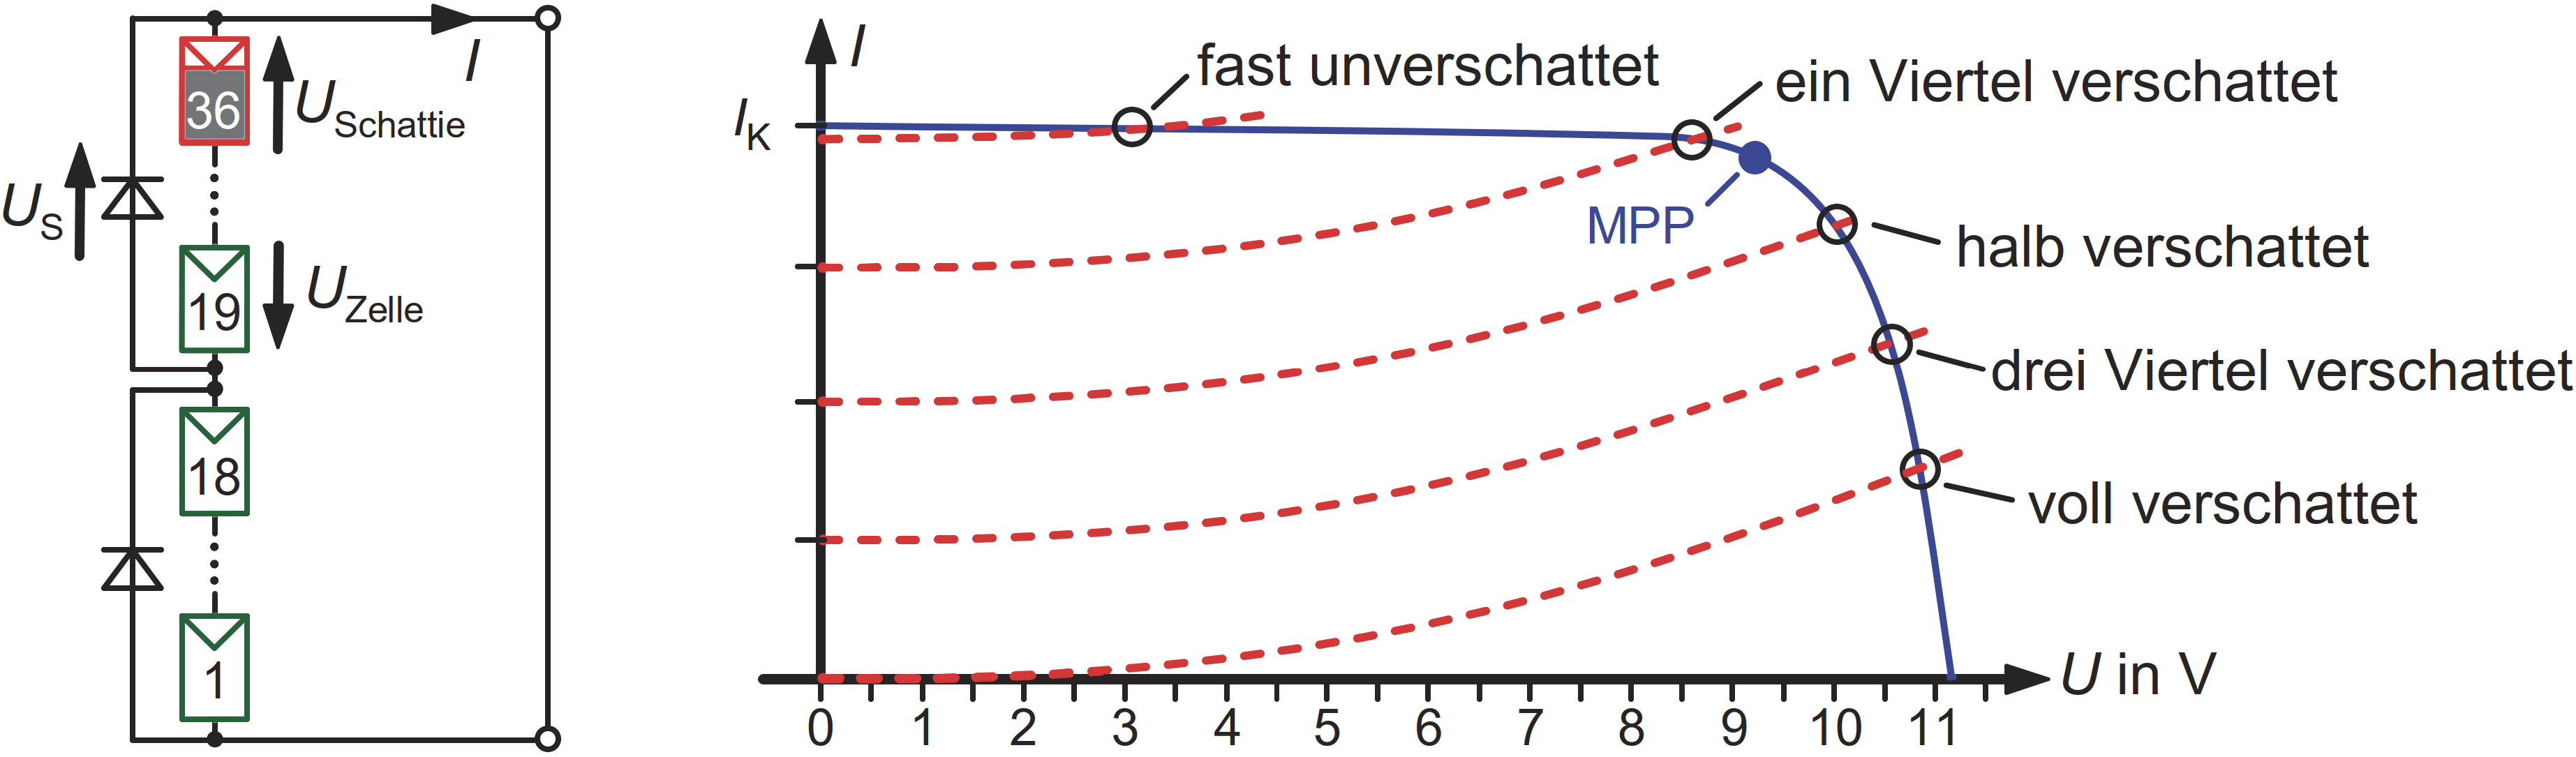
\includegraphics[width=0.95\columnwidth]{images/Vermeidung_von_Hotspots_3.png}



\subsubsection{Keine Hotspots bei Parallelschaltung}
%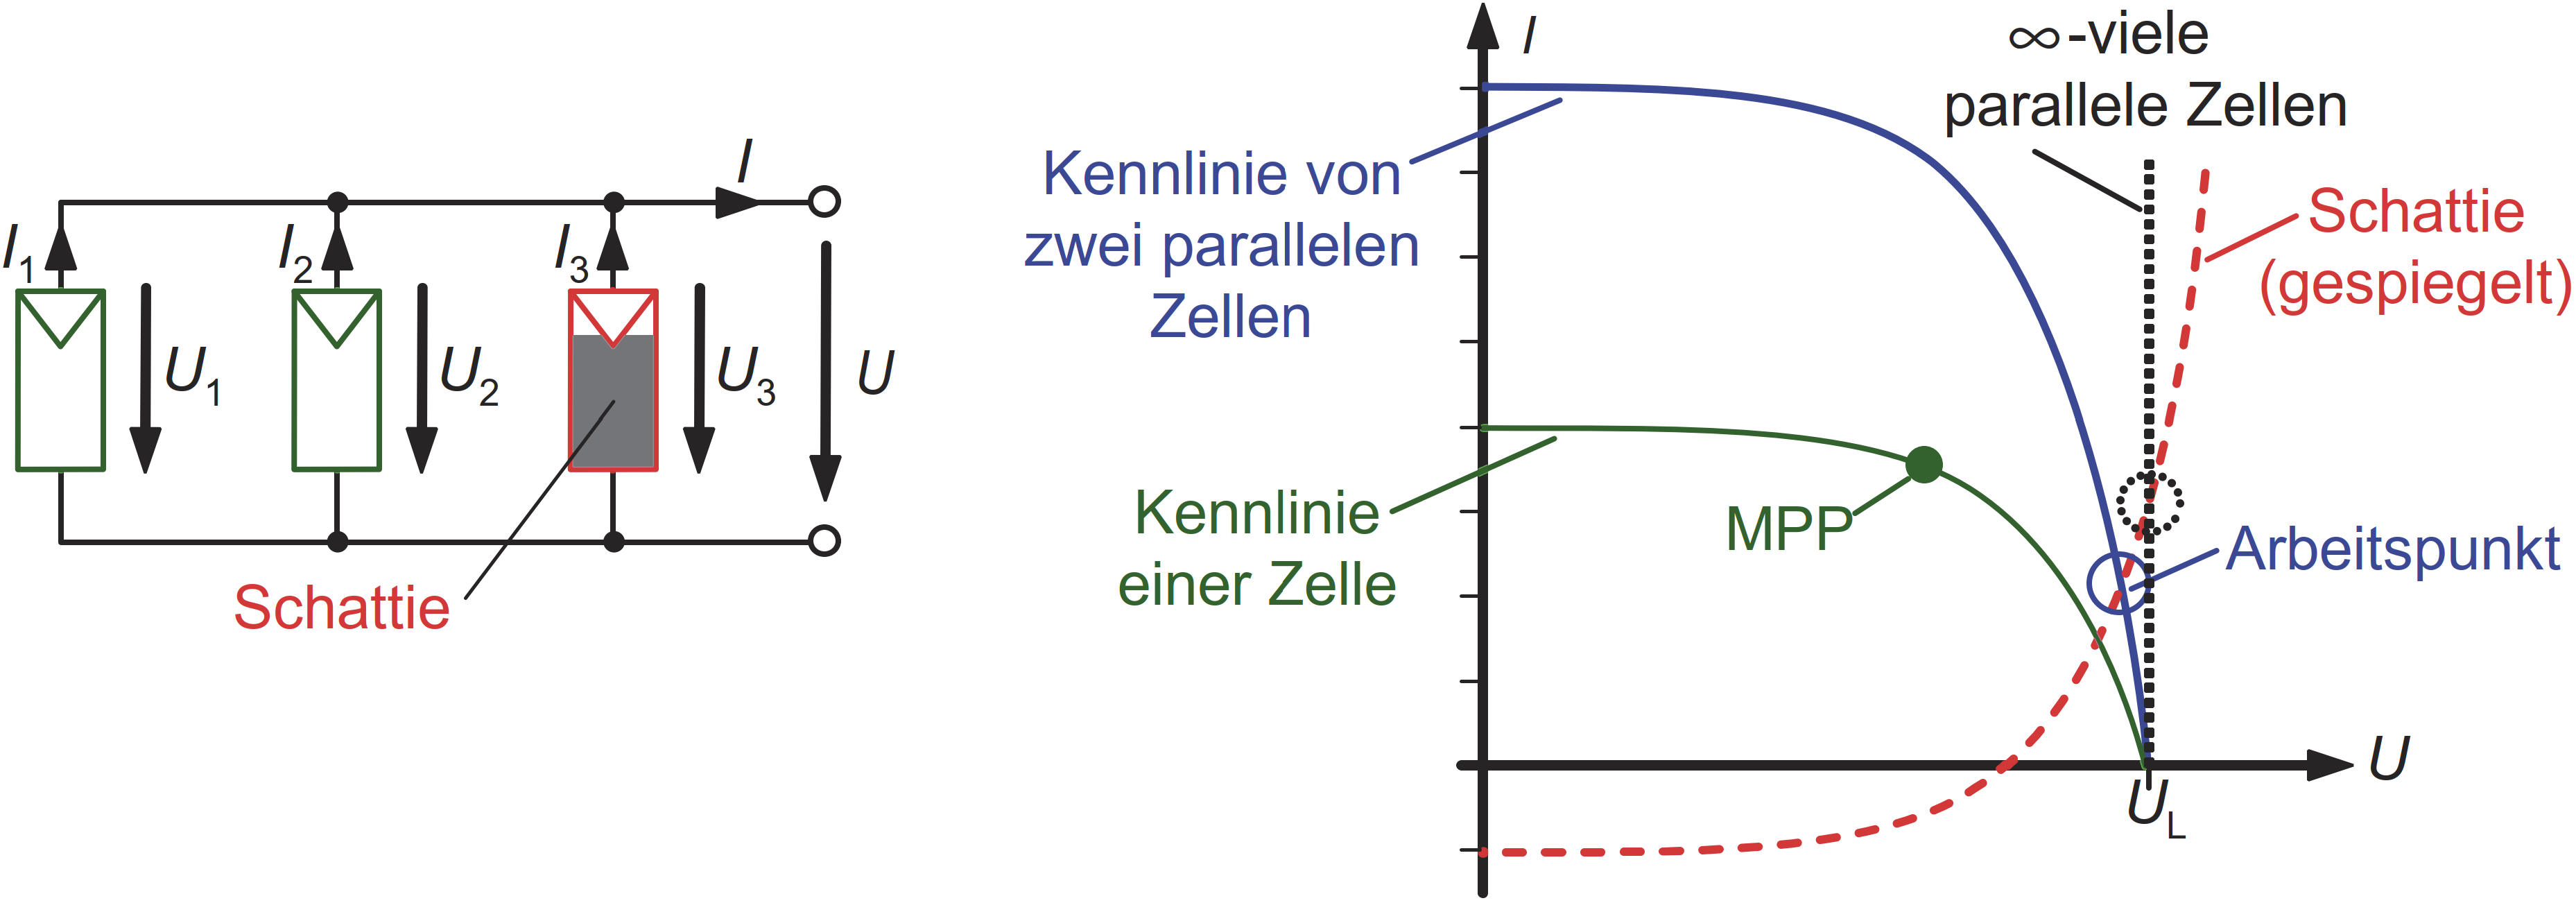
\includegraphics[width=0.95\columnwidth]{images/Keine_Hotspots_bei_Paralellschaltung.png}
        \columnbreak
\section{Einfluss von Einstrahlung und Temperatur}



\subsection{Standardtestbedingungen (STC - Standard Test Conditions)}
\textbf{Einheitliche Bedingungen für die Bestimmung der Nennleistung von Solarmodulen}

\vspace{0.1cm}

$\boxed{\mathrm{Einstrahlung:\,\,\,} G_{STC} = 1000 \, \frac{\mathrm{W}}{\mathrm{m^2}}}$

$\boxed{\mathrm{Zelltemperatur:\,\,\,} \vartheta_{\mathrm{Zell},\mathrm{STC}} = 25 \, {^\circ \mathrm{C}}}$

$\boxed{\text{Luftmasse AM:\,\,\,} 1.5}$

\subsection{Leistung in Abhängigkeit von Einstrahlung und Temperatur}

Die Leistung $P_{MPP}$ am Maximum Power Point (MPP) einer Solarzelle berechnet sich nach folgender Formel:

$\boxed{
P_{\mathrm{MPP}} = P_{\mathrm{STC}} \cdot \frac{G}{G_{\mathrm{STC}}} \cdot \left[1 + \alpha_{\mathrm{P}} \cdot \left(\vartheta_{\mathrm{Zell}} - \vartheta_{\mathrm{Zell},\mathrm{STC}}\right) \right]
}$

\vspace{0.1cm}

\begin{minipage}[c]{0.43\columnwidth}
    \renewcommand{\arraystretch}{1.2}
    \begin{tabular}{@{} l p{2.5cm} l @{}}
        $[P_{\mathrm{MPP}}]$              & MPP-Leistung \dotfill                & $\mathrm{W}$ \\
        $[P_{\mathrm{STC}}]$              & STC-Leistung \dotfill           & $\mathrm{W}$ \\
        $[G]$                             & Globalstrahlung \dotfill                                 & $\frac{\mathrm{W}}{\mathrm{m^2}}$ \\
        $[G_{\mathrm{STC}}]$              & Globalstr. bei STC \dotfill            & $\frac{\mathrm{W}}{\mathrm{m^2}}$ 
    \end{tabular}
\end{minipage}
\hfill
\vrule width 1pt
\hfill
\begin{minipage}[c]{0.49\columnwidth}
    \renewcommand{\arraystretch}{1.2}
    \begin{tabular}{@{} l p{2.6cm} l @{}}
        $[\alpha_{\mathrm{P}}]$           & Leistungs Temp-koeff \dotfill              & $\frac{\%}{^\circ\mathrm{C}}$ \\
        $[\vartheta_{\mathrm{Zell}}]$     & Zelltemperatur \dotfill                                  & $^\circ\mathrm{C}$ \\
        $[\vartheta_{\mathrm{Zell},\mathrm{STC}}]$ & Zelltemp bei STC \dotfill & $^\circ\mathrm{C}$ 
    \end{tabular}
\end{minipage}



\subsection{Strom und Spannung (Einstrahlung und Temperatur)}

Die Abhängigkeit von Strom und Spannung einer Solarzelle von der Einstrahlung und Temperatur wird durch folgende Gleichungen beschrieben:

\vspace{0.1cm}

$\boxed{
I_{\mathrm{K}} = I_{\mathrm{K},\mathrm{STC}} \cdot \frac{G}{G_{\mathrm{STC}}} \cdot \left[1 + \alpha_{\mathrm{I}} \cdot \left(\vartheta_{\mathrm{Zell}} - \vartheta_{\mathrm{Zell},\mathrm{STC}}\right) \right]
}$\quad \textcolor{red}{!$\alpha$ Unterschiedlich!}

$\boxed{
U_{\mathrm{L}} = U_{\mathrm{L},\mathrm{Grafik}} \cdot \left[1 + \alpha_{\mathrm{U}} \cdot \left(\vartheta_{\mathrm{Zell}} - \vartheta_{\mathrm{Zell},\mathrm{STC}}\right) \right]
}$

$\boxed{
I_{\mathrm{MPP}} = I_{\mathrm{MPP},\mathrm{STC}} \cdot \frac{G}{G_{\mathrm{STC}}} \cdot \left[1 + \alpha_{\mathrm{I}} \cdot \left(\vartheta_{\mathrm{Zell}} - \vartheta_{\mathrm{Zell},\mathrm{STC}}\right) \right]
}$

$\boxed{
U_{\mathrm{MPP}} = \frac{P_{\mathrm{MPP}}}{I_{\mathrm{MPP}}}
}$\quad \textcolor{red}{Spannung immer über P \& I}

$\boxed{
R_{\mathrm{P\_max}} = \frac{U_{\mathrm{MPP}}}{I_{\mathrm{MPP}}}
}$\quad \textcolor{red}{Spannung immer über P \& I}

\vspace{0.1cm}

\renewcommand{\arraystretch}{1.2} % Erhöht Zeilenhöhe für bessere Lesbarkeit
\begin{tabular}{@{} l p{7cm} l @{}}
    $[I_{\mathrm{K}}]$                           & Kurzschlussstrom ($G$, $[\vartheta_{\mathrm{Zell}}]$) \dotfill                & $\mathrm{A}$ \\
    $[I_{\mathrm{K},\mathrm{STC}}]$              & Kurzschlussstrom bei Standardtestbedingungen \dotfill                         & $\mathrm{A}$ \\
    $[U_{\mathrm{L}}]$                           & Leerlaufspannung ($G$, $[\vartheta_{\mathrm{Zell}}]$) \dotfill                & $\mathrm{V}$ \\
    $[U_{\mathrm{L},\mathrm{Grafik}}]$           & Leerlaufspannung ($G$) aus Grafik \dotfill                                    & $\mathrm{V}$ \\
    $[I_{\mathrm{MPP}}]$                         & Strom im Maximum Power Point ($G$, $[\vartheta_{\mathrm{Zell}}]$) \dotfill    & $\mathrm{A}$ \\
    $[I_{\mathrm{MPP},\mathrm{STC}}]$            & Strom im Maximum Power Point bei STC \dotfill                                 & $\mathrm{A}$ \\
    $[U_{\mathrm{MPP}}]$                         & Spannung im Maximum Power Point ($G$, $[\vartheta_{\mathrm{Zell}}]$) \dotfill & $\mathrm{V}$ \\
    $[G]$                                        & Globalstrahlung \dotfill                                                      & $\frac{\mathrm{W}}{\mathrm{m^2}}$ \\
    $[G_{\mathrm{STC}}]$                         & Globalstrahlung bei STC = 1000\,W/m² \dotfill                                 & $\frac{\mathrm{W}}{\mathrm{m^2}}$ \\
    $[\alpha_{\mathrm{I}}]$                      & Temperaturkoeffizient des Kurzschlussstroms \dotfill                          & $\frac{\%}{^\circ\mathrm{C}}$ \\
    $[\alpha_{\mathrm{U}}]$                      & Temperaturkoeffizient der Leerlaufspannung \dotfill                           & $\frac{\%}{^\circ\mathrm{C}}$ \\
    $[\vartheta_{\mathrm{Zell}}]$                & Zelltemperatur \dotfill                                                       & $^\circ\mathrm{C}$ \\
    $[\vartheta_{\mathrm{Zell},\mathrm{STC}}]$   & Zelltemperatur bei STC = $25^\circ\mathrm{C}$ \dotfill                        & $^\circ\mathrm{C}$ \\
\end{tabular}
        \columnbreak
\section{Serien- und Parallelschaltung von Zellen und Modulen}
\textcolor{red}{$U_{\mathrm{LL}}$ ändert bei Verschattung nur minimal! Änderung fast nur an $I_{\mathrm{K}}$.}

\subsection{Serienschaltung von Solarzellen}
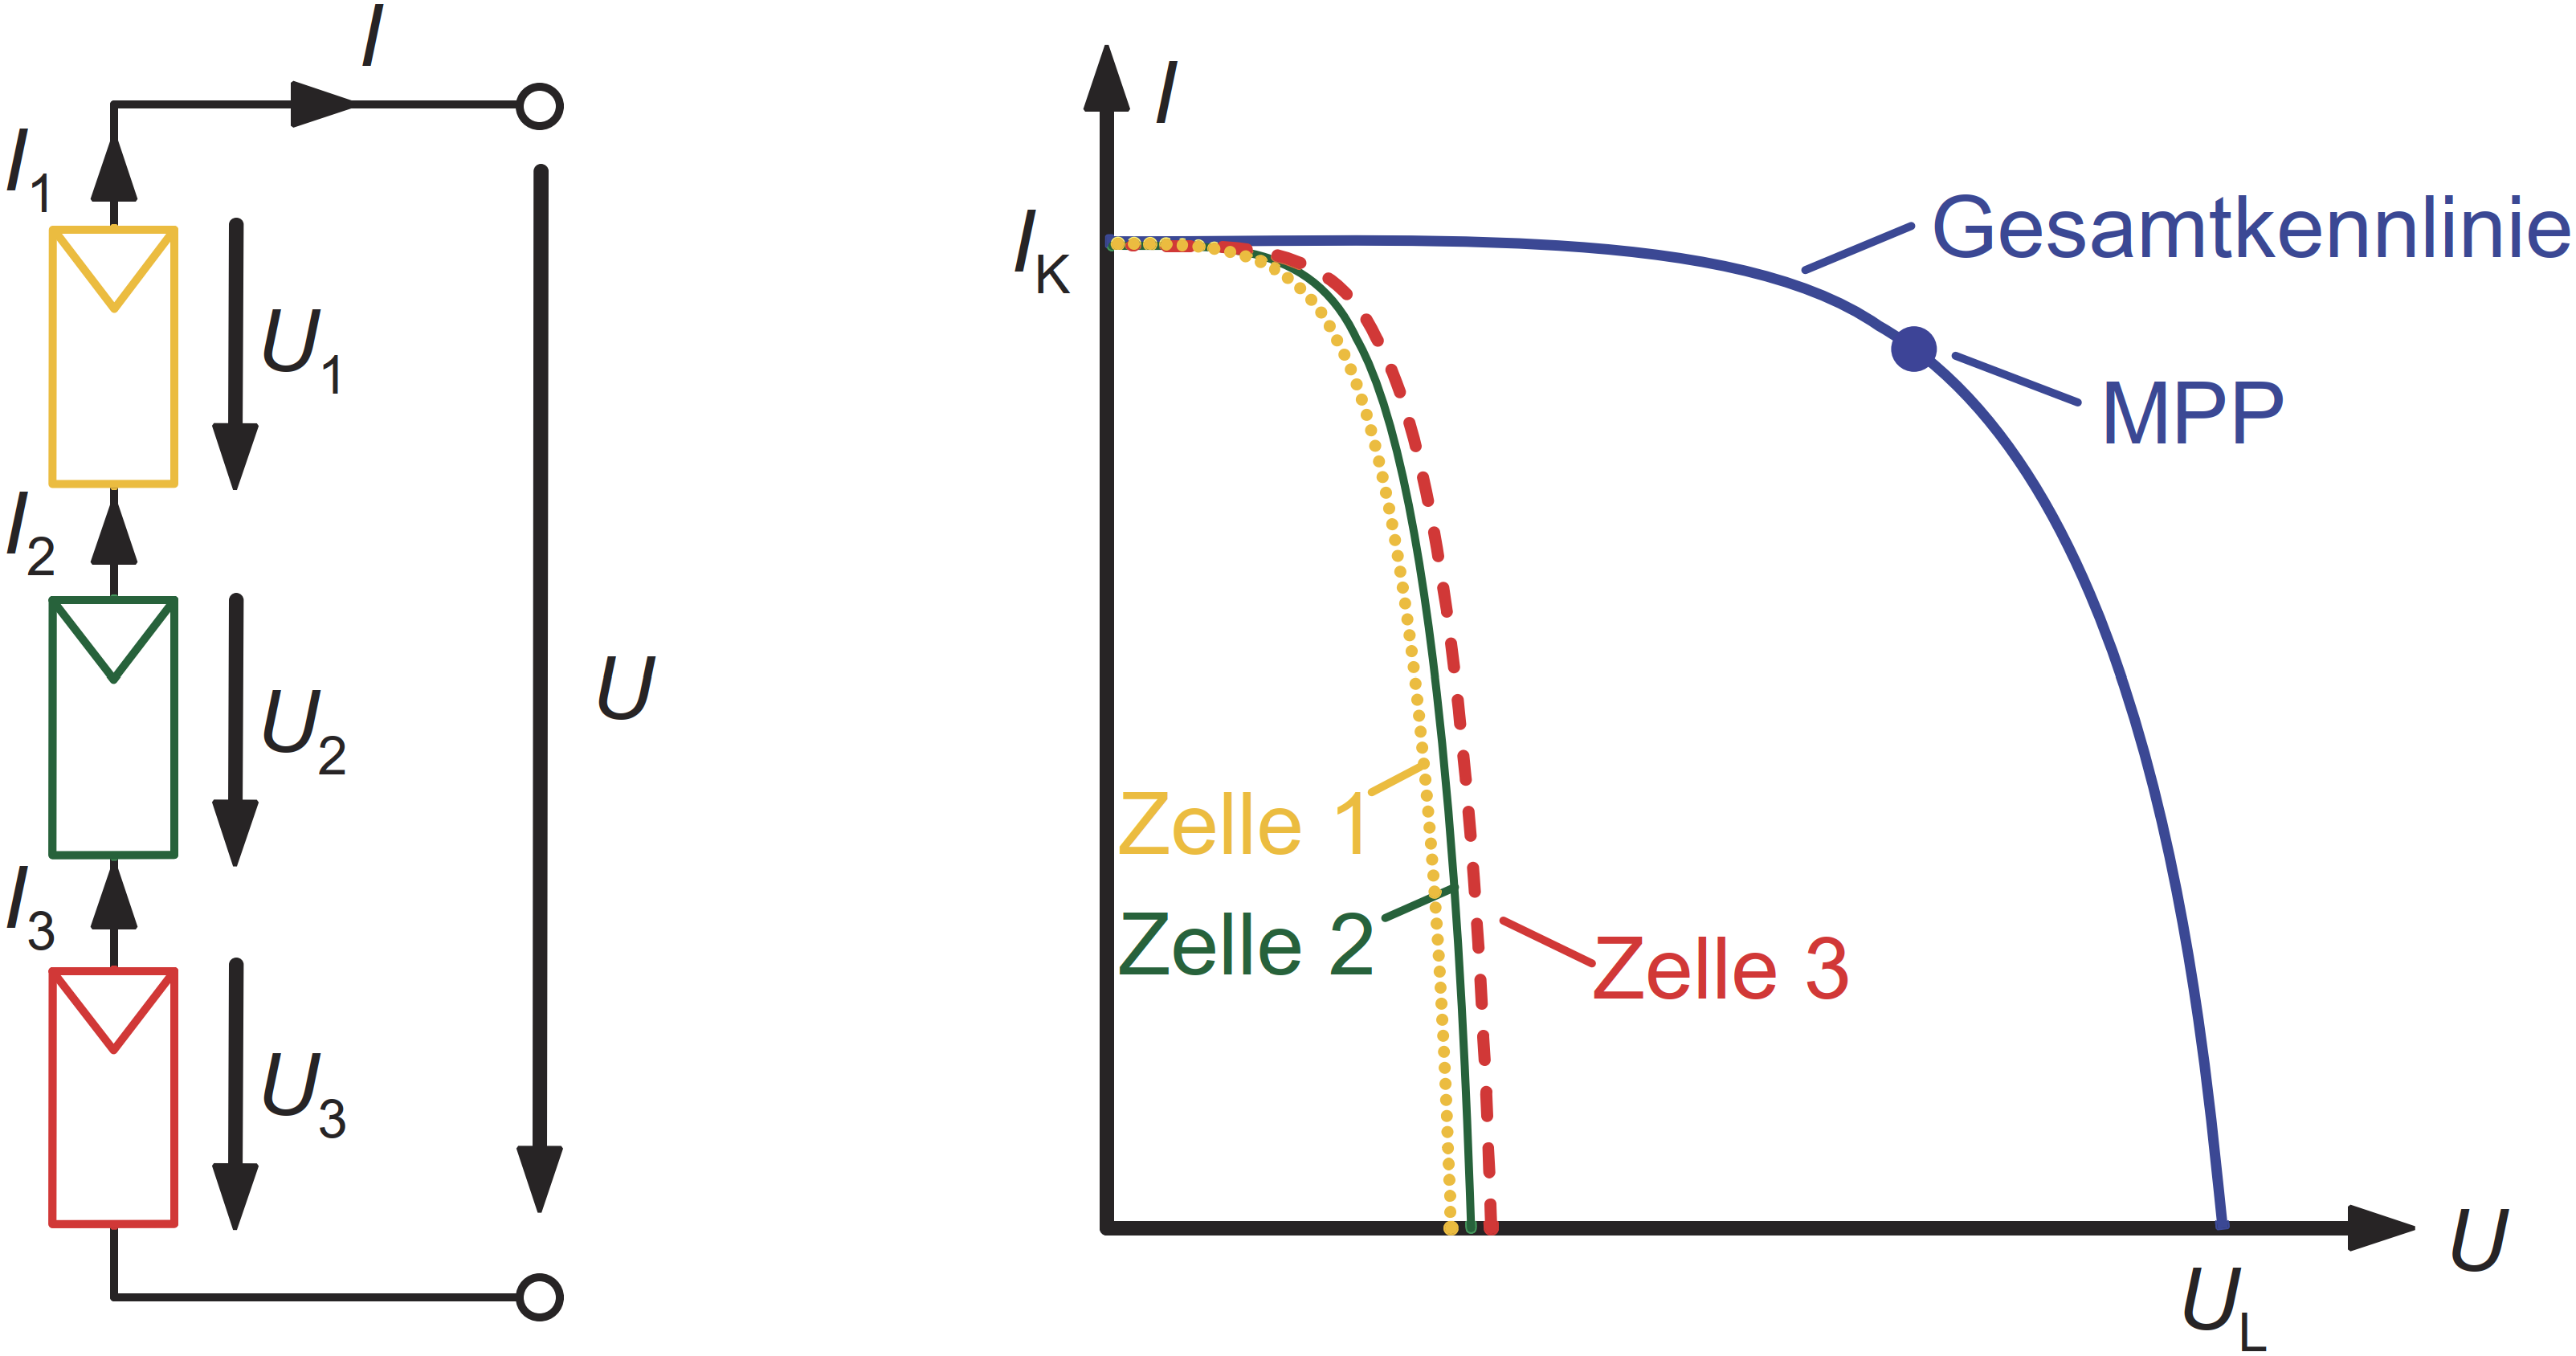
\includegraphics[width=0.7\columnwidth]{images/Serienschaltung_von_Solarzellen.png}


\subsubsection{Serienschaltung mit verschatteter Zelle}
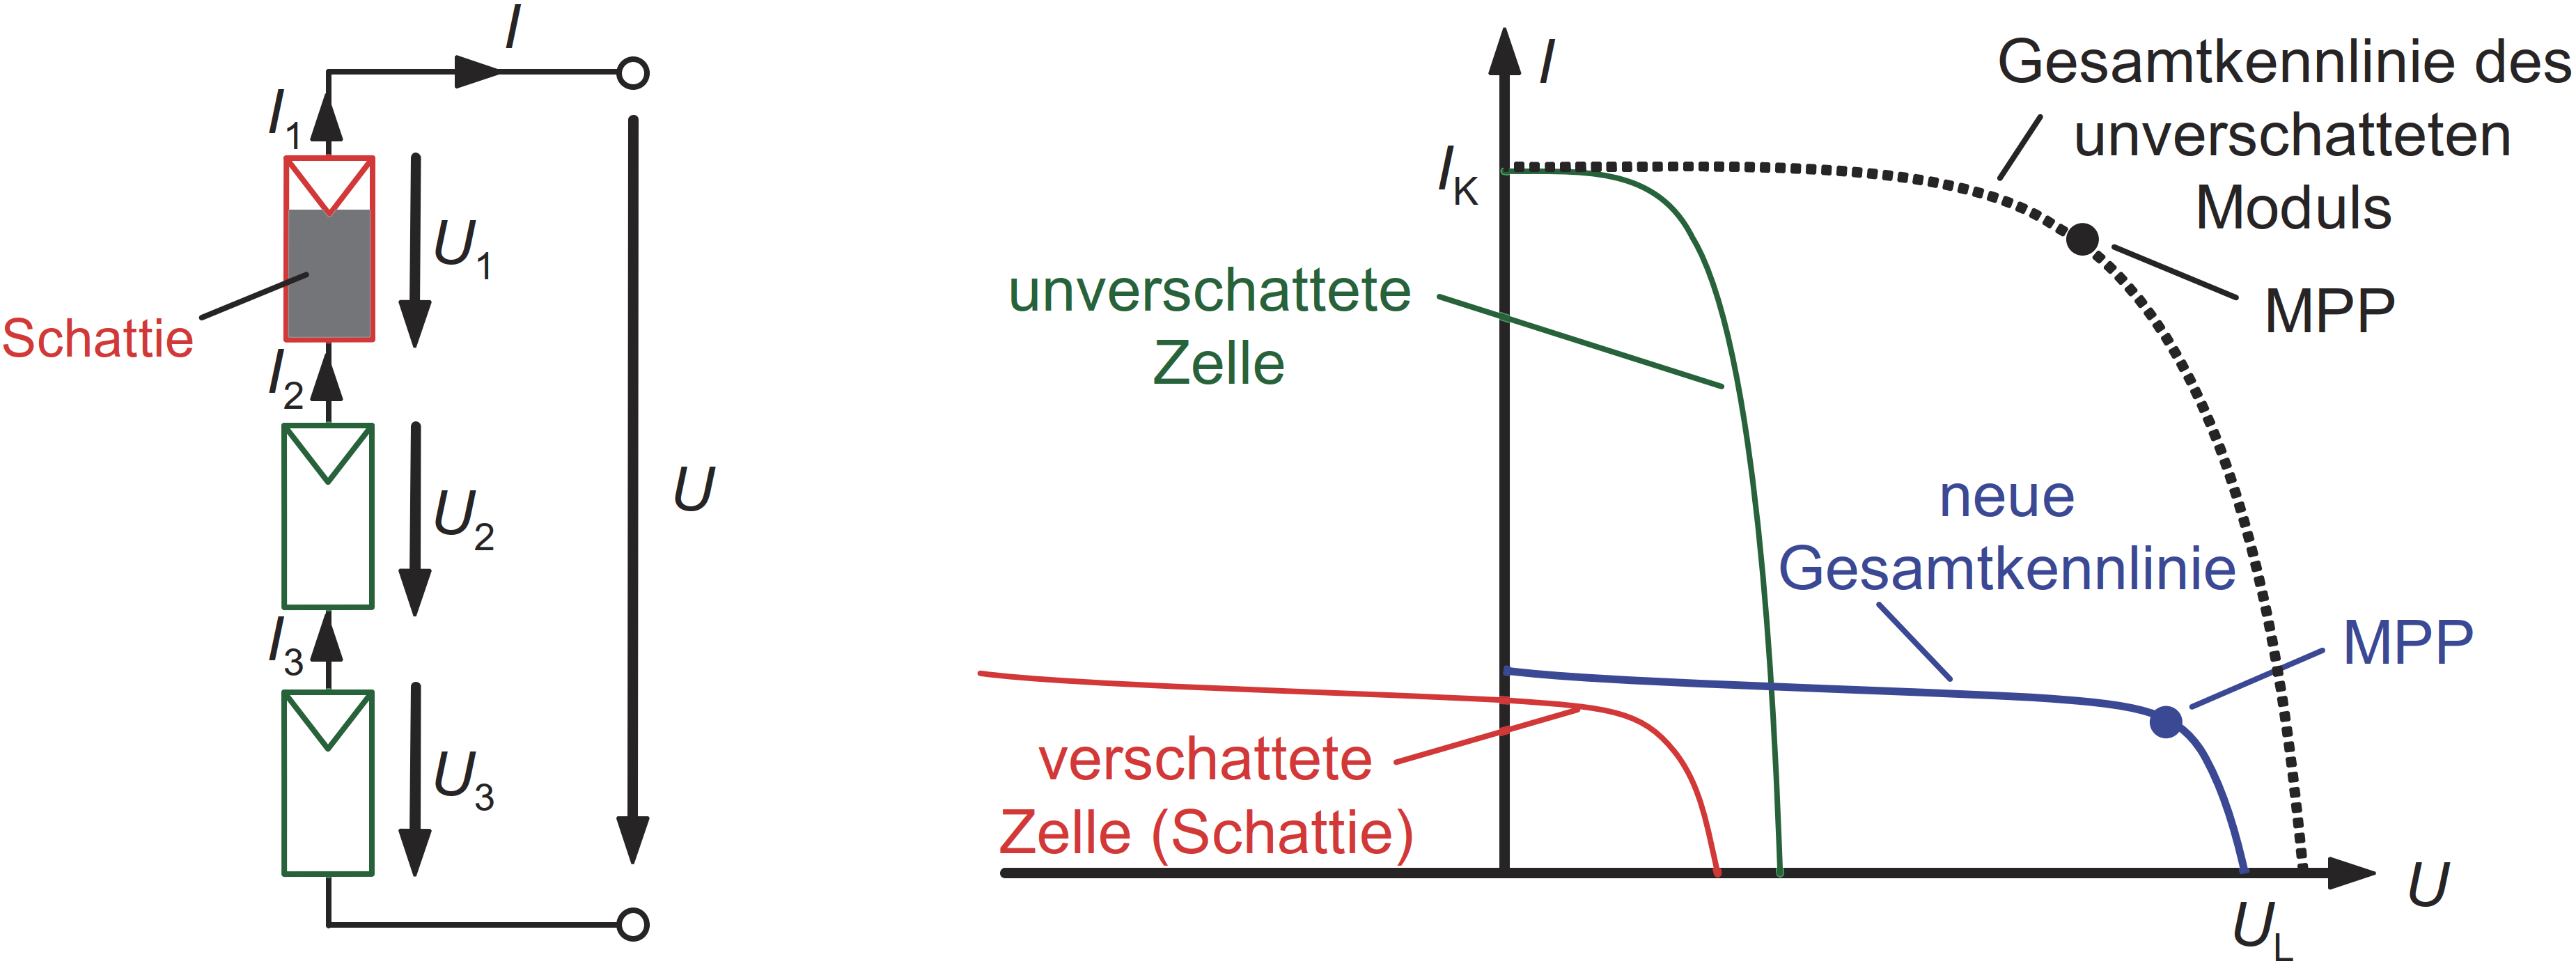
\includegraphics[width=0.98\columnwidth]{images/Serienschaltung_von_Solarzellen_mit_verschatteter_Zelle.png}


\subsection{Parallelschaltung von Solarzellen}
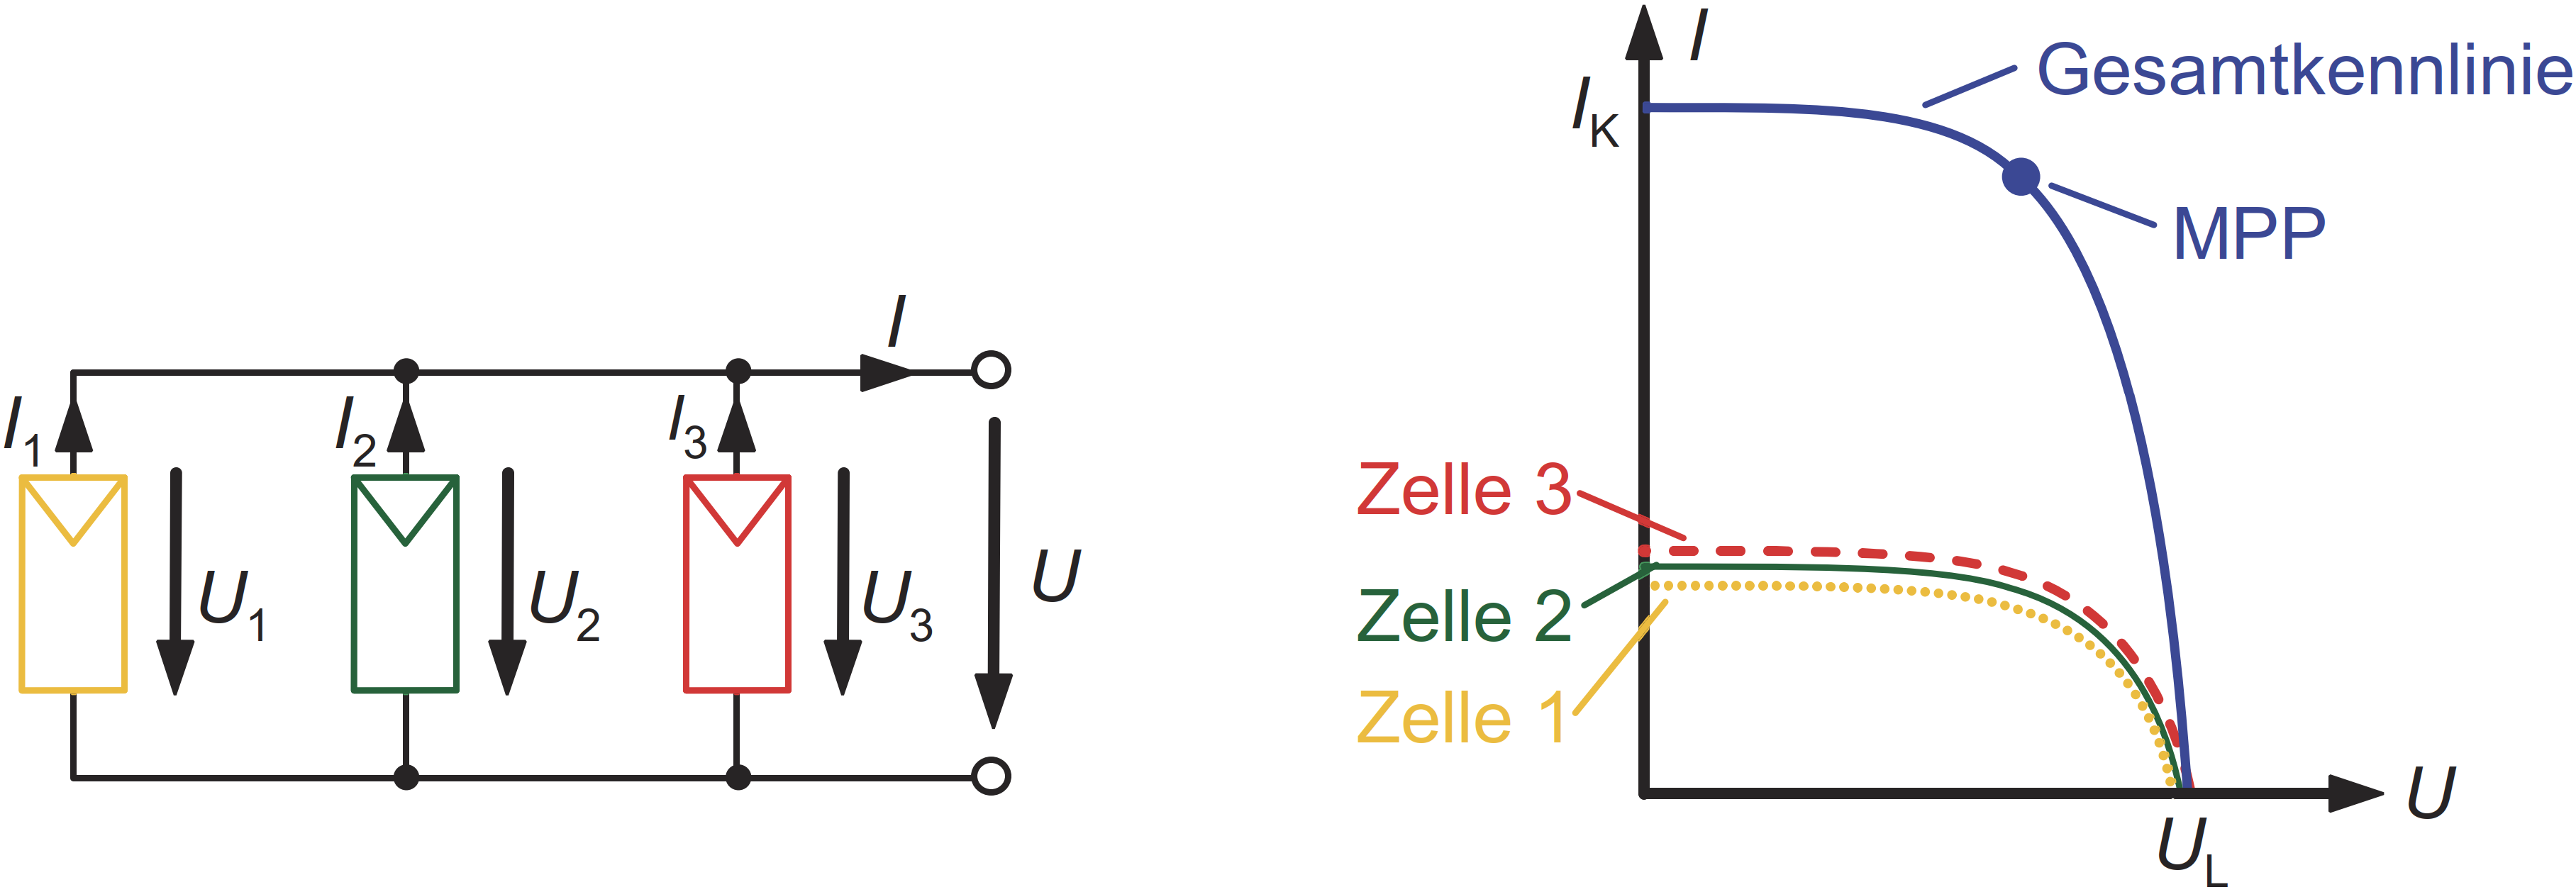
\includegraphics[width=0.95\columnwidth]{images/Parallelschaltung_von_Solarzellen.png}

\subsubsection{Parallelschaltung mit verschatteter Zelle}
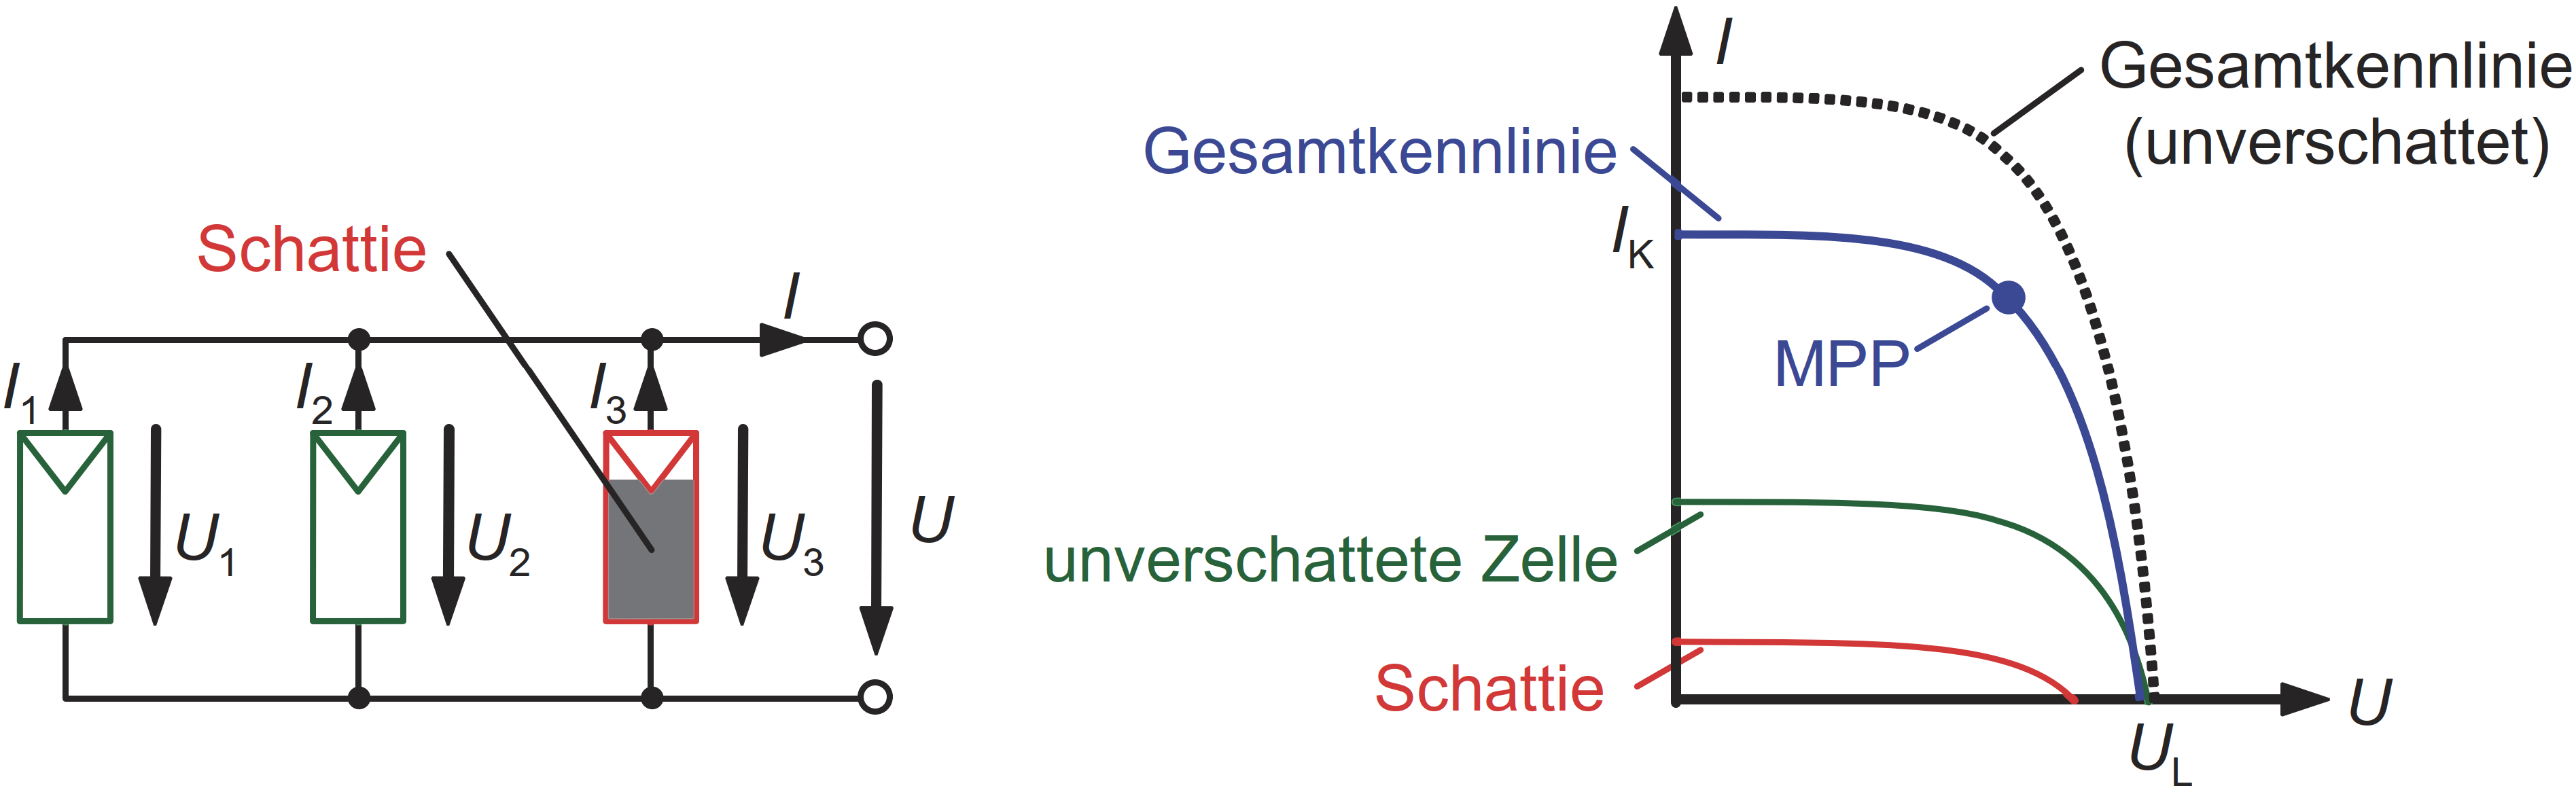
\includegraphics[width=0.95\columnwidth]{images/Parallelschaltung_von_Solarzellen_mit_verschatteter_Zelle.png}


\subsection{Beispiel aus Übungen}
Zwei Solarmodule mit den Daten \( U_L = 43{,}2\,\mathrm{V} \) und \( I_K = 10\,\mathrm{A} \) werden in Serie geschaltet. Modul A wird mit \( 1\,000\,\mathrm{W/m^2} \) bestrahlt, Modul B mit \( 500\,\mathrm{W/m^2} \). Skizzieren Sie die Einzelkurven und die Gesamtkurve für die Fälle:

\begin{enumerate}[label=\alph*.]
    \item Die Module haben keine Bypassdioden.
    \item Beide Module haben mindestens eine Bypassdiode.
\end{enumerate}

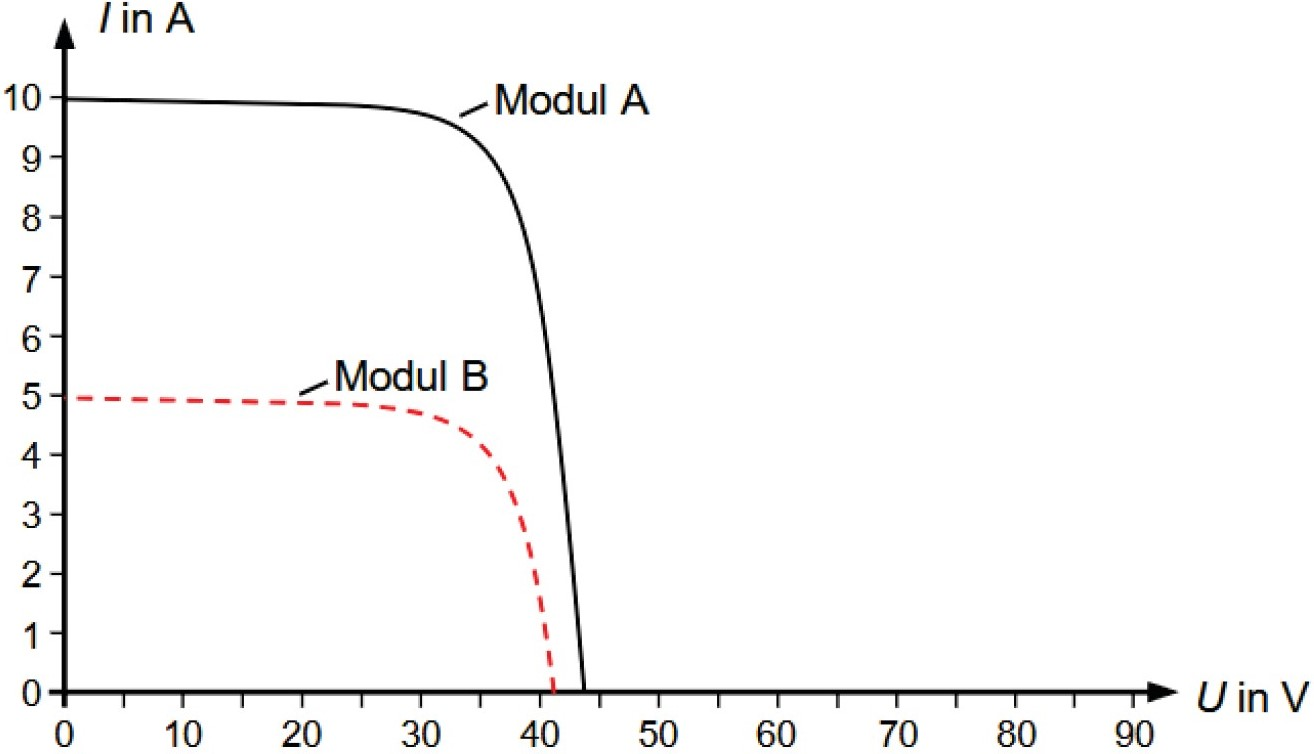
\includegraphics[width=0.6\columnwidth]{images/Beispiel_1.jpg}

\vspace{0.1cm}

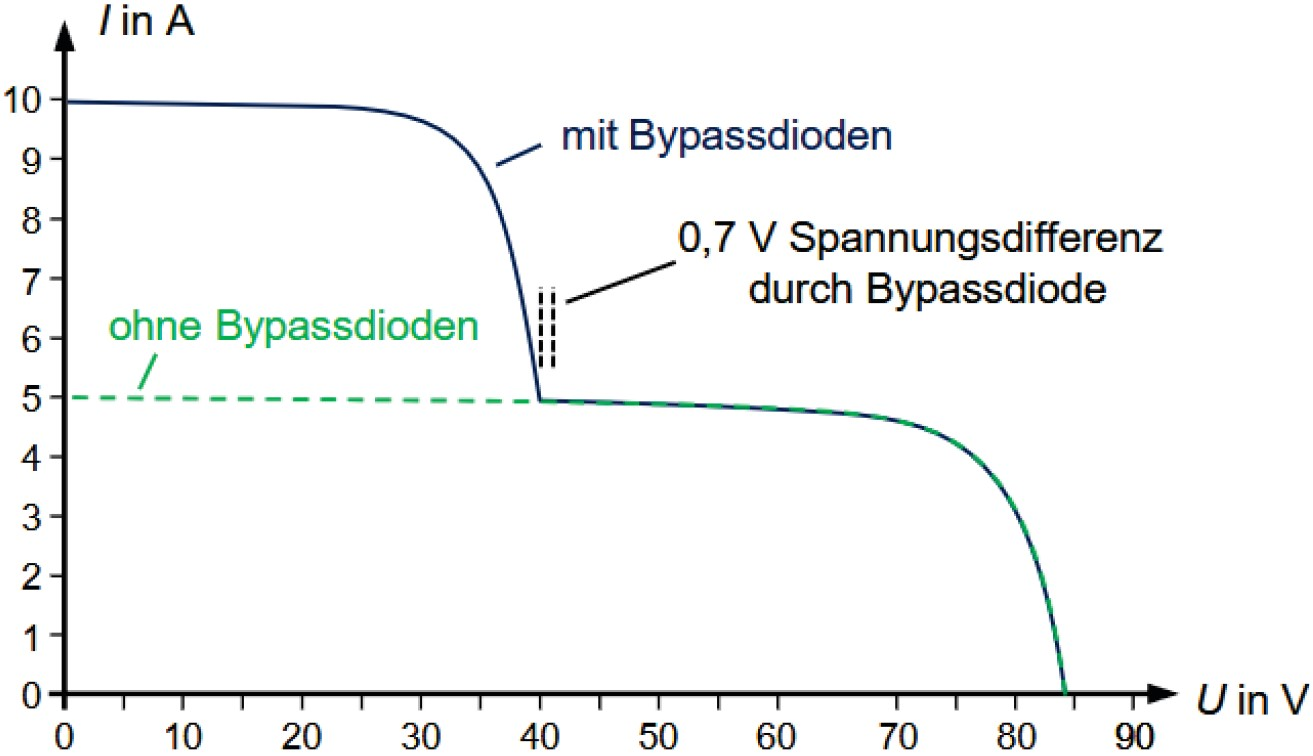
\includegraphics[width=0.6\columnwidth]{images/Beispiel_2.jpg}
















        \columnbreak
\section{Gleichstrom Komponenten}
%\begin{comment}
\subsection{Aufbau PV-Anlage}
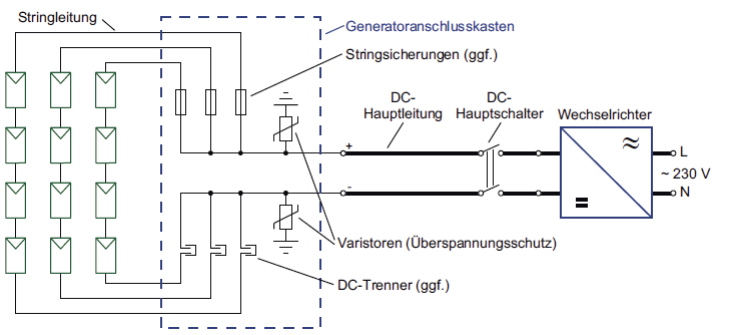
\includegraphics[width=0.95\columnwidth]{images/Aufbau_PV-Anlage.png}

\subsection{Gleichstromverkabelung}
\subsubsection{Solarstecker}

\begin{itemize}
    \item MC4 Solarstecker (quasi Standard)
\end{itemize}

\begin{minipage}[t]{0.48\columnwidth}
    \myul{\textbf{MC4}}\\
    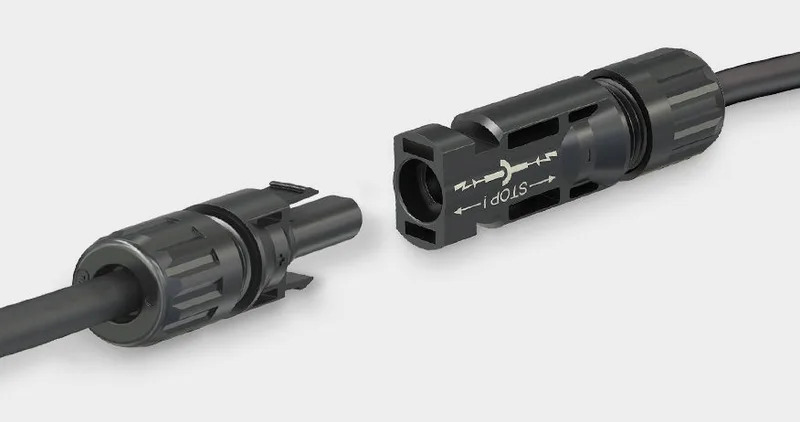
\includegraphics[width=0.95\columnwidth]{images/MC4.jpg}
\end{minipage}
\hfill
\begin{minipage}[t]{0.48\columnwidth}
    \myul{\textbf{MC4-Evo 2000}}\\
    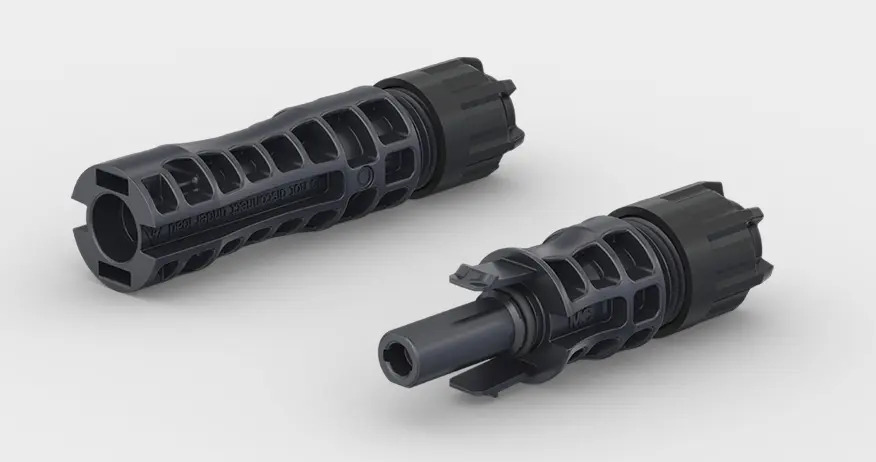
\includegraphics[width=0.95\columnwidth]{images/MC4-Evo 2000.jpg}
\end{minipage}

\vspace{0.25cm}

\subsubsection{Gleichstromkabel}

\begin{minipage}[t]{0.48\columnwidth}
    \myul{\textbf{MC FLEX-SOL-EVO-DX}}\\
    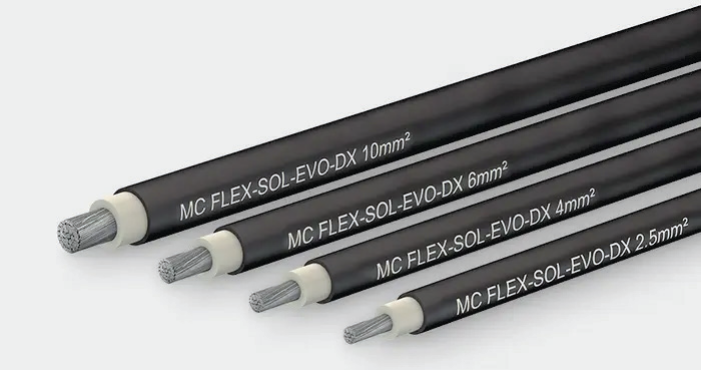
\includegraphics[width=0.95\columnwidth]{images/MC_FLEX-SOL-EVO-DX.png}
\end{minipage}
\hfill
\begin{minipage}[t]{0.48\columnwidth}
    \myul{\textbf{Anforderungen}}\\
    \begin{itemize}
        \item Doppelte Isolation\\
                (Schutz gegen Kurzschluss)
        \item UV-Beständigkeit
        \item Schwer entflammbar 
        \item Für hohe Temperaturen
\end{itemize}
\end{minipage}
%\end{comment}


\subsection{Tiefstellsetzer, Buck-Converter}

\begin{minipage}[c]{0.48\columnwidth}
    \begin{center}
        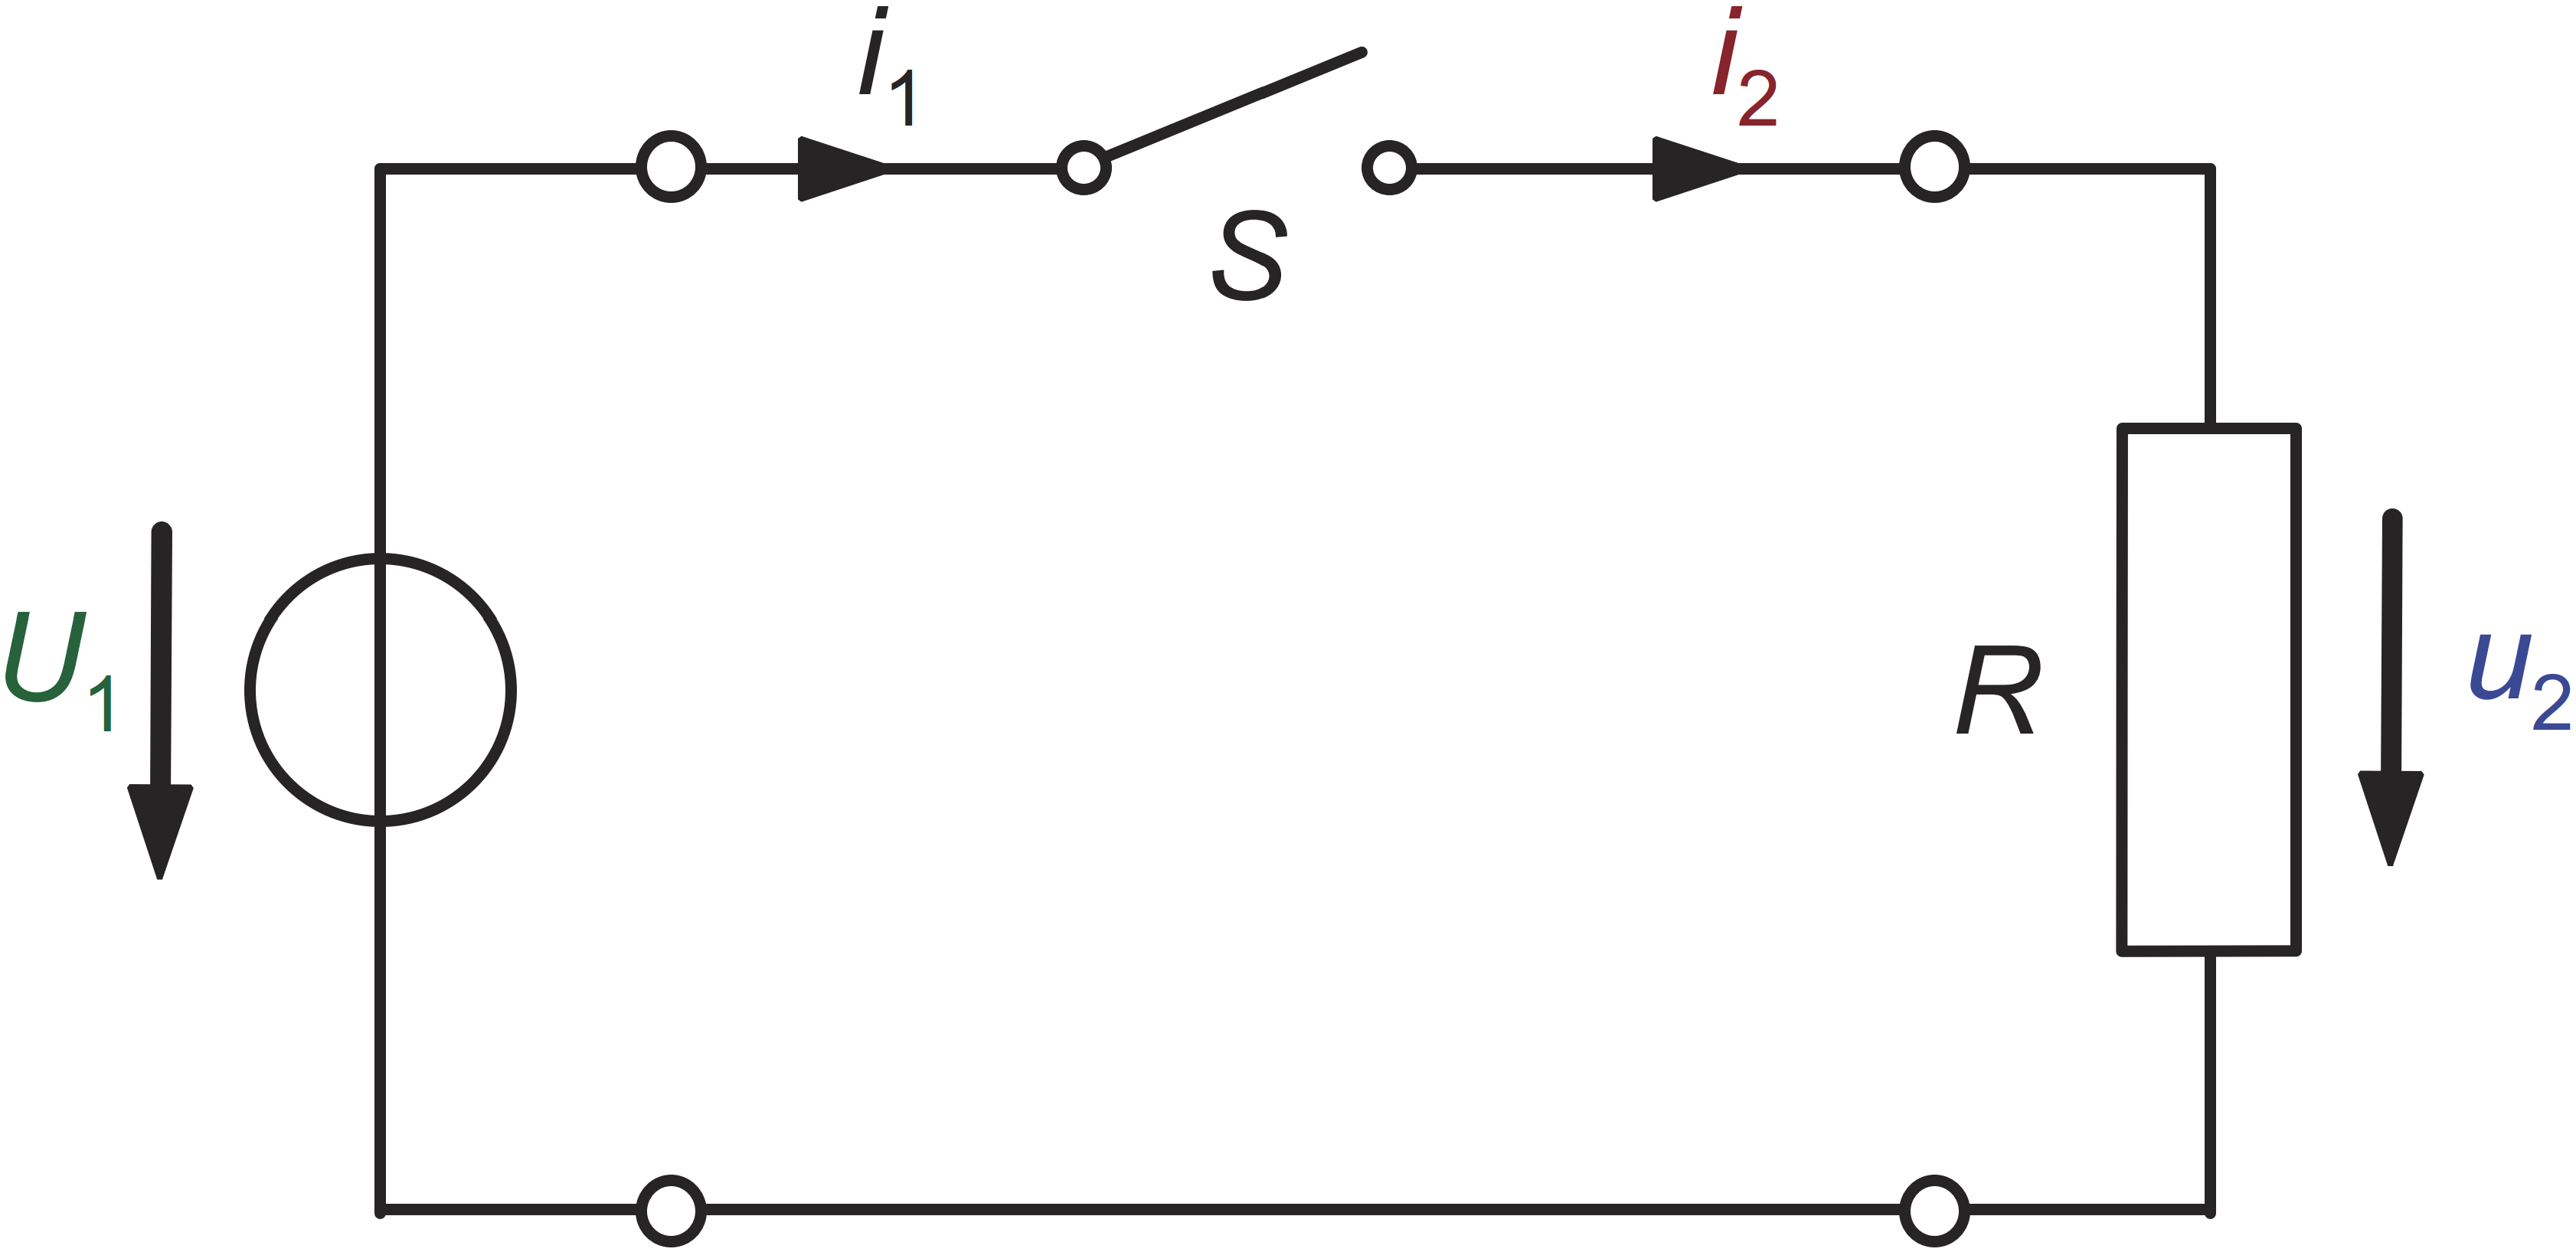
\includegraphics[width=1\columnwidth]{images/Tiefsetzsteller_Vereinfacht.png} 
    \end{center}
\end{minipage}
\hfill
\begin{minipage}[c]{0.48\columnwidth}
    \begin{center}
        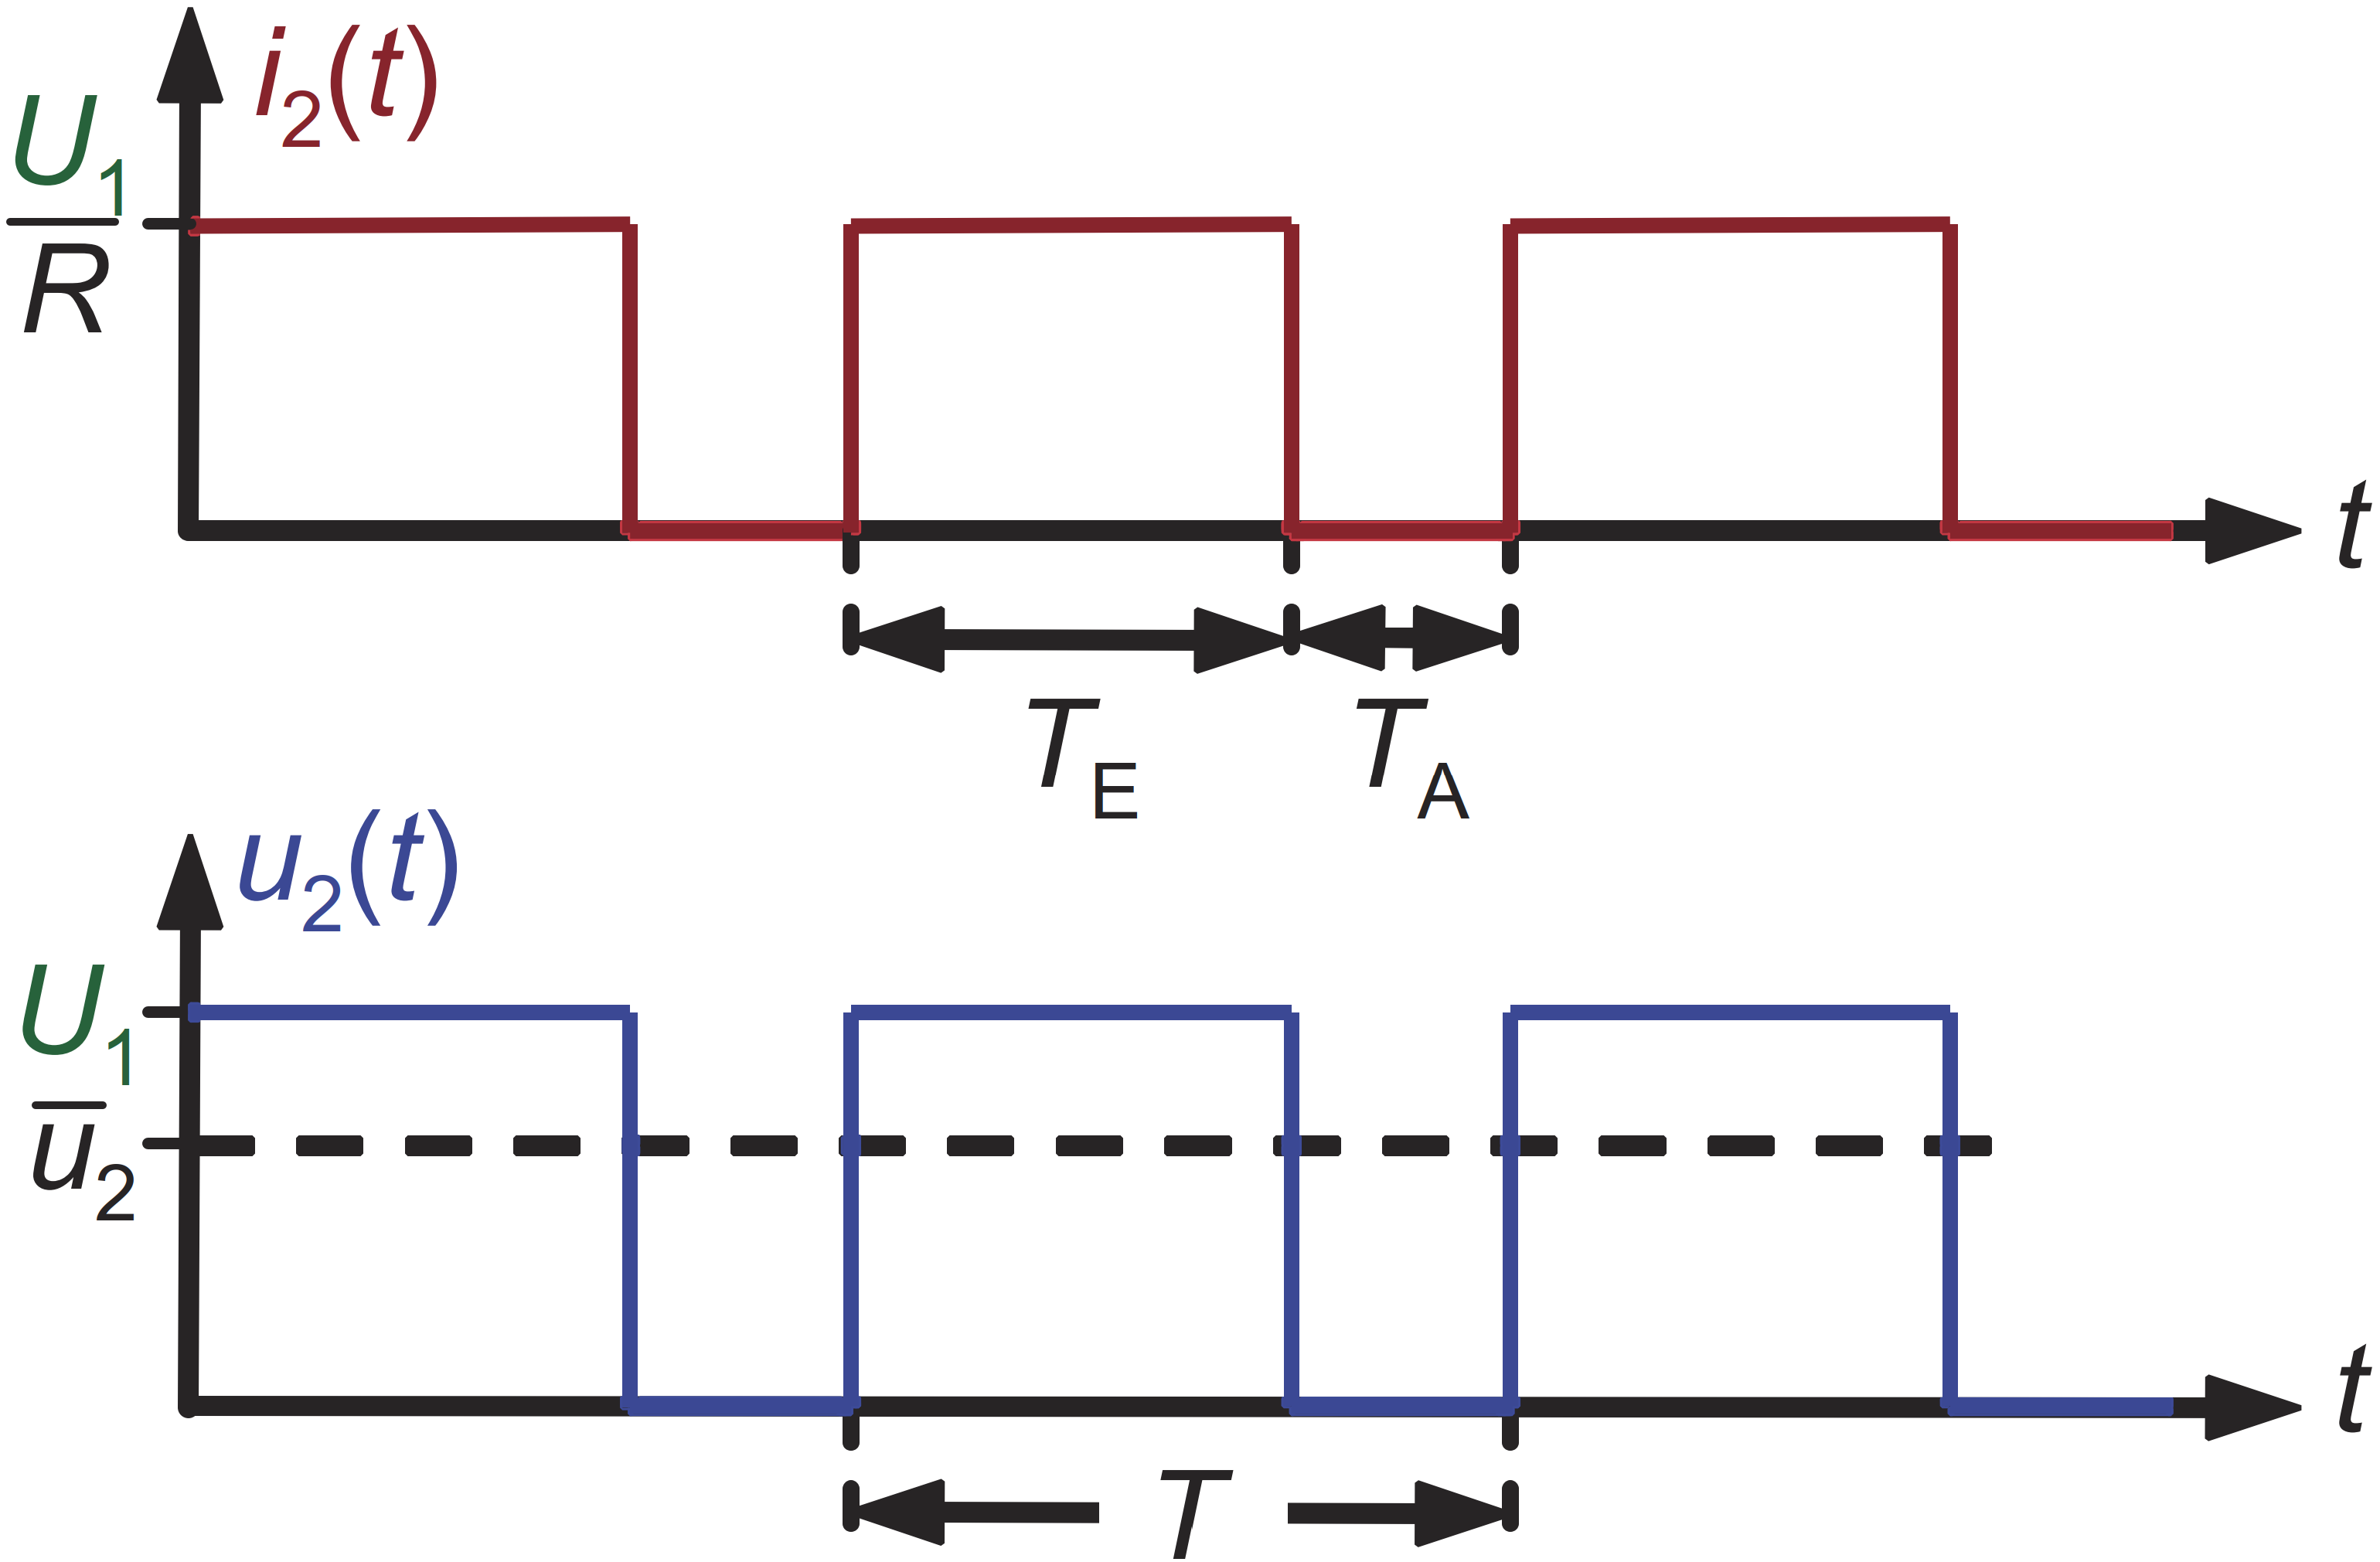
\includegraphics[width=0.95\columnwidth]{images/Tiefsetzsteller_DutyCycle.png}
    \end{center}
\end{minipage}



$
\boxed{
\bar{u}_2 = \frac{T_E}{T} \cdot U_1 = a \cdot U_1
}
$
\quad
$
\boxed{
a = \frac{T_E}{T}
}
$
\quad
$
\boxed{T = T_E +T_A}
$

\begin{minipage}[t]{0.48\columnwidth}
    \renewcommand{\arraystretch}{1.2}
\begin{tabular}{@{} l p{3.1cm} l @{}}
    $[T]$                   & Periodendauer PWM \dotfill          & $\mathrm{s}$ \\
    $[T_{\mathrm{E}}]$      & Einschaltdauer PWM \dotfill         & $\mathrm{s}$ \\
    $[T_{\mathrm{A}}]$      & Ausschaltdauer PWM \dotfill         & $\mathrm{s}$ \\
    $[U_1]$                 & Eingangsspannung \dotfill               & $\mathrm{V}$ \\
    $[a]$                   & Tastgrad (Duty Cycle) \dotfill          & $-$ \\
\end{tabular}
\end{minipage}
\hfill
\vrule width 1pt
\hfill
\begin{minipage}[t]{0.48\columnwidth}
    \renewcommand{\arraystretch}{1.2}
\begin{tabular}{@{} l p{3.1cm} l @{}}
    $[U_2]$                 & Ausgangsspannung \dotfill               & $\mathrm{V}$ \\
    $[u_{\mathrm{D}}]$      & Spannung über Diode \dotfill            & $\mathrm{V}$ \\
    $[u_{\mathrm{L}}]$      & Spannung über Spule \dotfill            & $\mathrm{V}$ \\
    $[i_{\mathrm{L}}]$      & Strom durch Spule \dotfill              & $\mathrm{A}$ \\
    $[L]$                   & Induktivität der Spule \dotfill         & $\mathrm{H}$ \\
\end{tabular}
\end{minipage}


\columnbreak
\subsubsection{Effektives Schema Tiefstellsetzer, Buck-Converter}
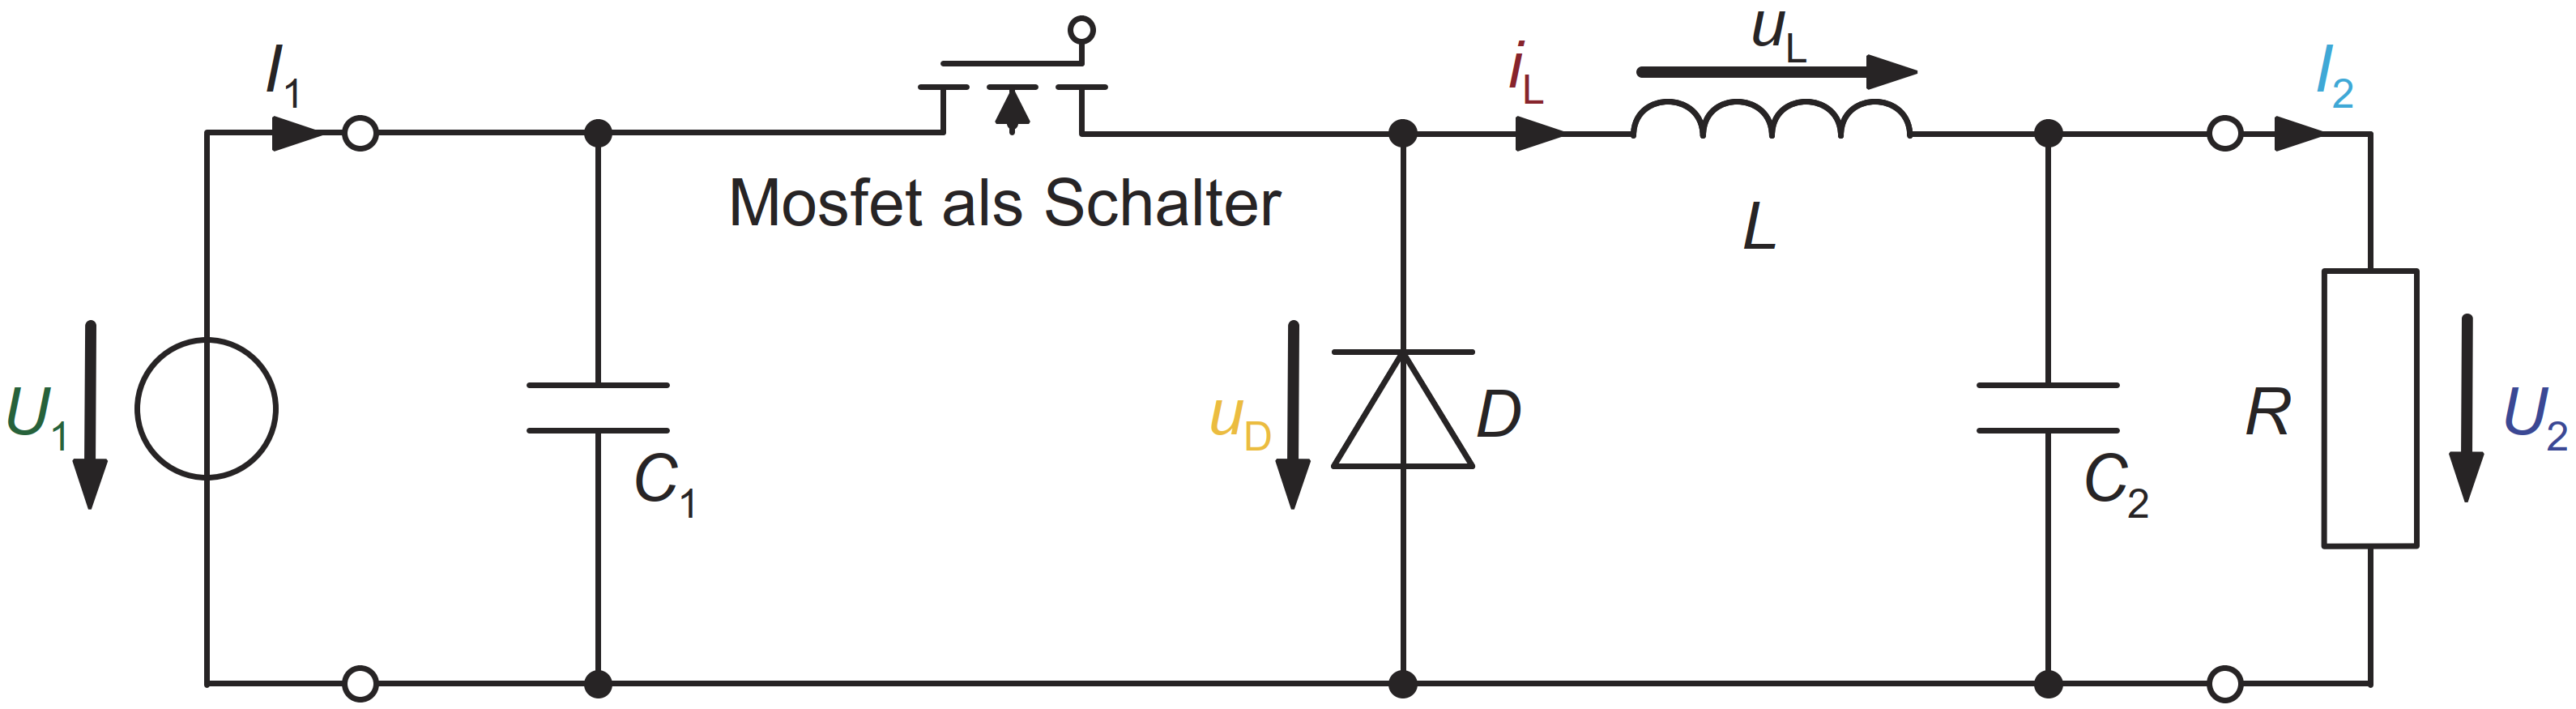
\includegraphics[width=1\columnwidth]{images/Tiefsetzsteller_1.png}

\vspace{0.25cm}

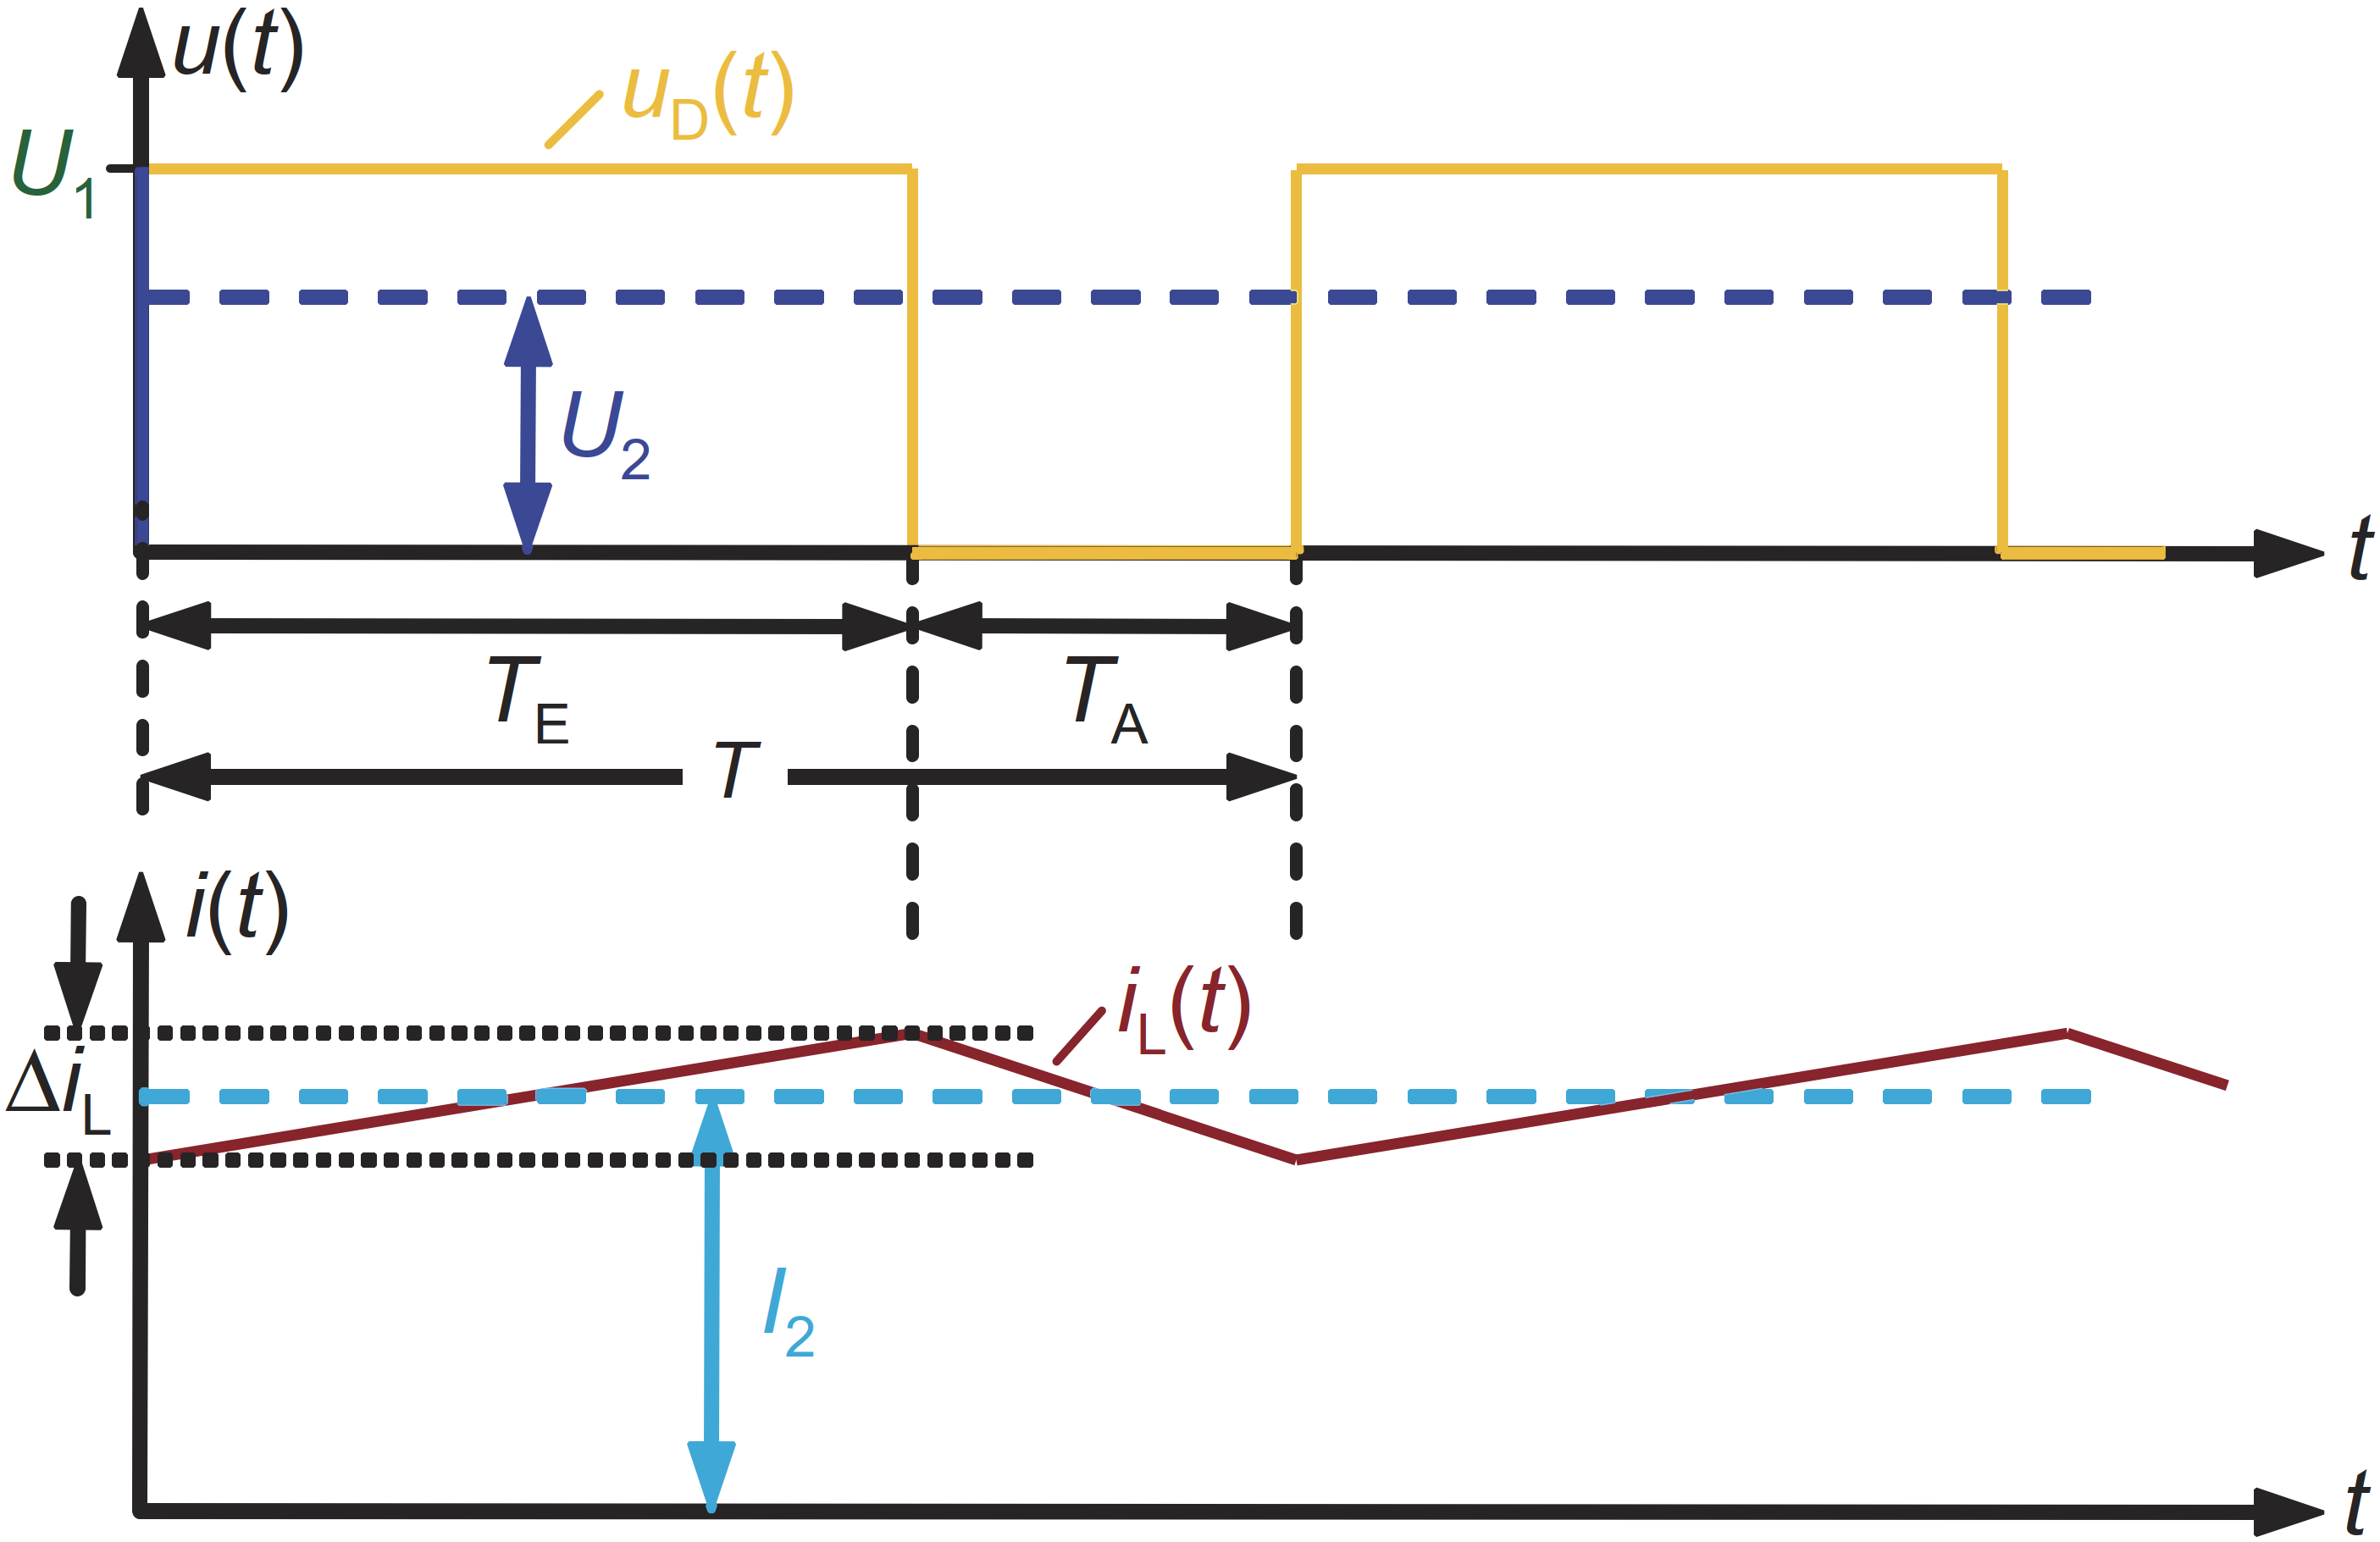
\includegraphics[width=0.8\columnwidth]{images/Tiefsetzsteller_2.png}

\vspace{0.25cm}

$
\boxed{u_D = U_1}
$
\quad
$
\boxed{u_L = u_D - U_2 = U_1 - U_2}
$
\quad
$
\boxed{u_L(t) = L \cdot \frac{\mathrm{d}i_L}{\mathrm{d}t}}
$
\quad
$
\boxed{U_2 = a \cdot U_1}
$

\vspace{0.25cm}

\begin{minipage}[t]{0.48\columnwidth}
    \myul{\textbf{Strom Anstiegsgeschwindigkeit ($T_E$)}}\\
    $
        \boxed{\frac{\mathrm{d}i_L}{\mathrm{d}t} = \frac{u_L}{L} = \frac{U_1 - U_2}{L}}
    $
    \quad
    $t \in [0, T_E]$
\end{minipage}
\hfill
\begin{minipage}[t]{0.48\columnwidth}
    \myul{\textbf{Strom Abfallstiegsgeschwindigkeit ($T_A$)}}\\
    $
        \boxed{\frac{\mathrm{d}i_L}{\mathrm{d}t} = \frac{u_L}{L} = \frac{-U_2}{L}}
    $
    \quad
    $t \in [T_E, T_A]$
\end{minipage}

\vspace{0.25cm}

\subsection{Hochstellsetzer, Boost-Converter}

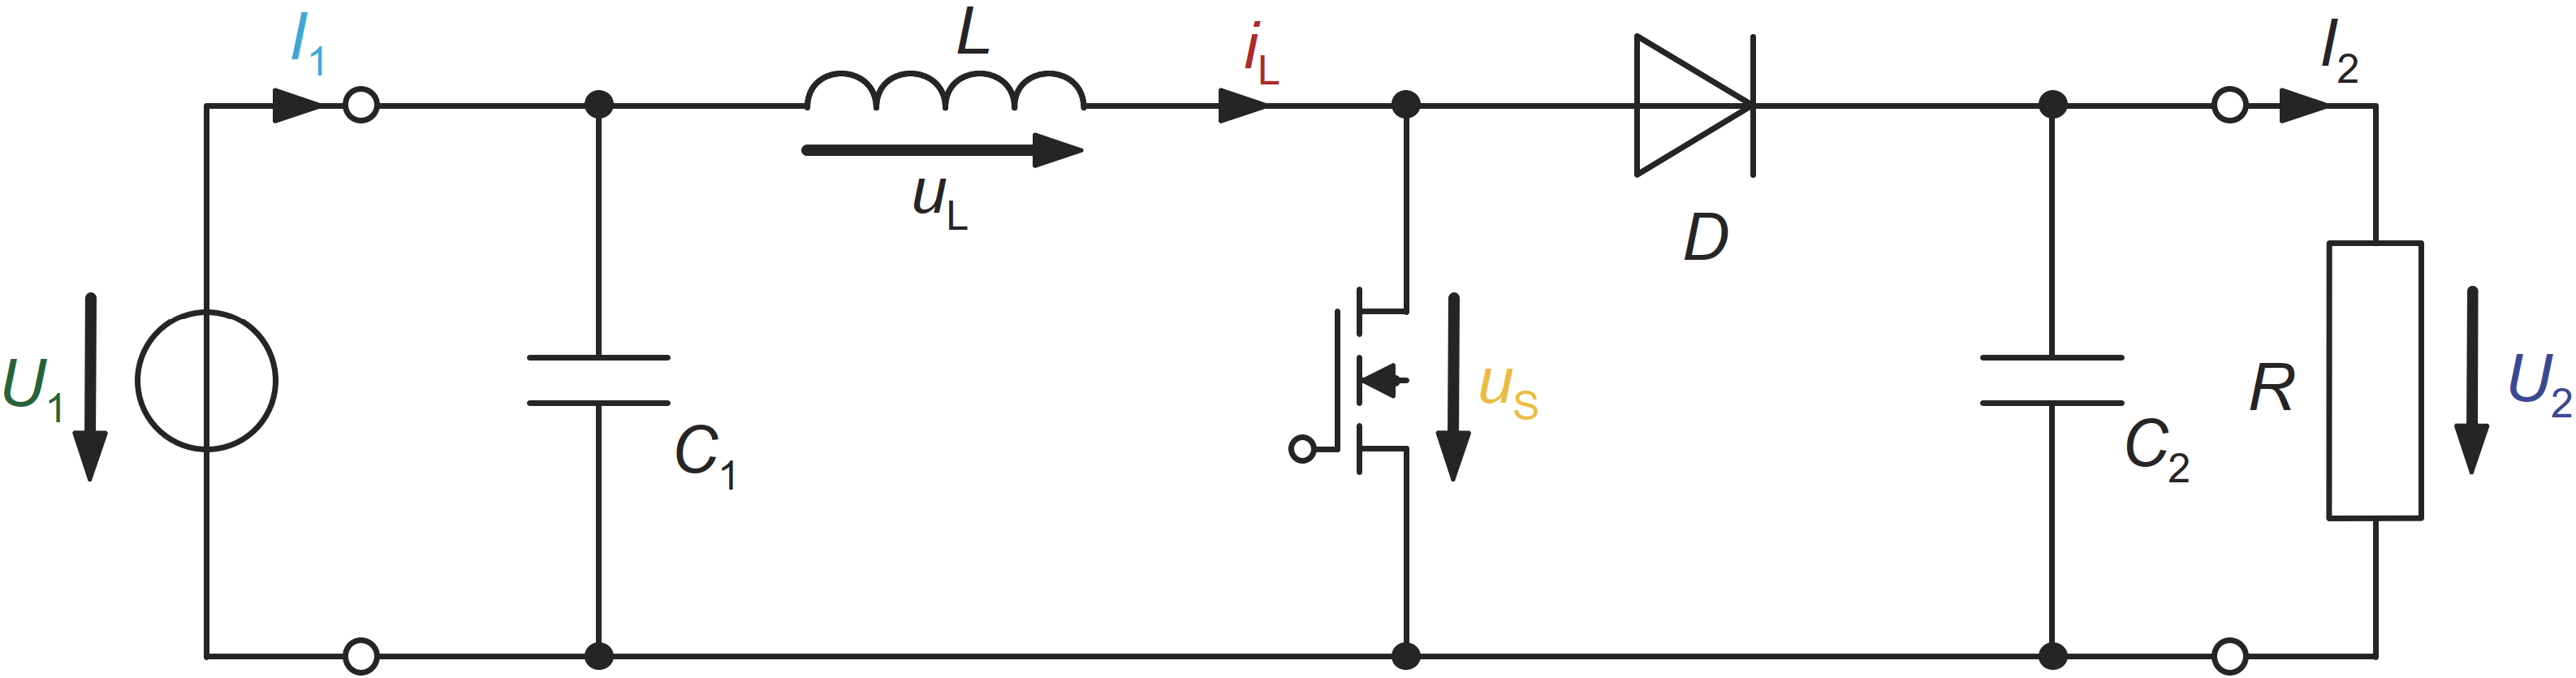
\includegraphics[width=1\columnwidth]{images/Hochstellsetzer_1.png}

\vspace{0.25cm}

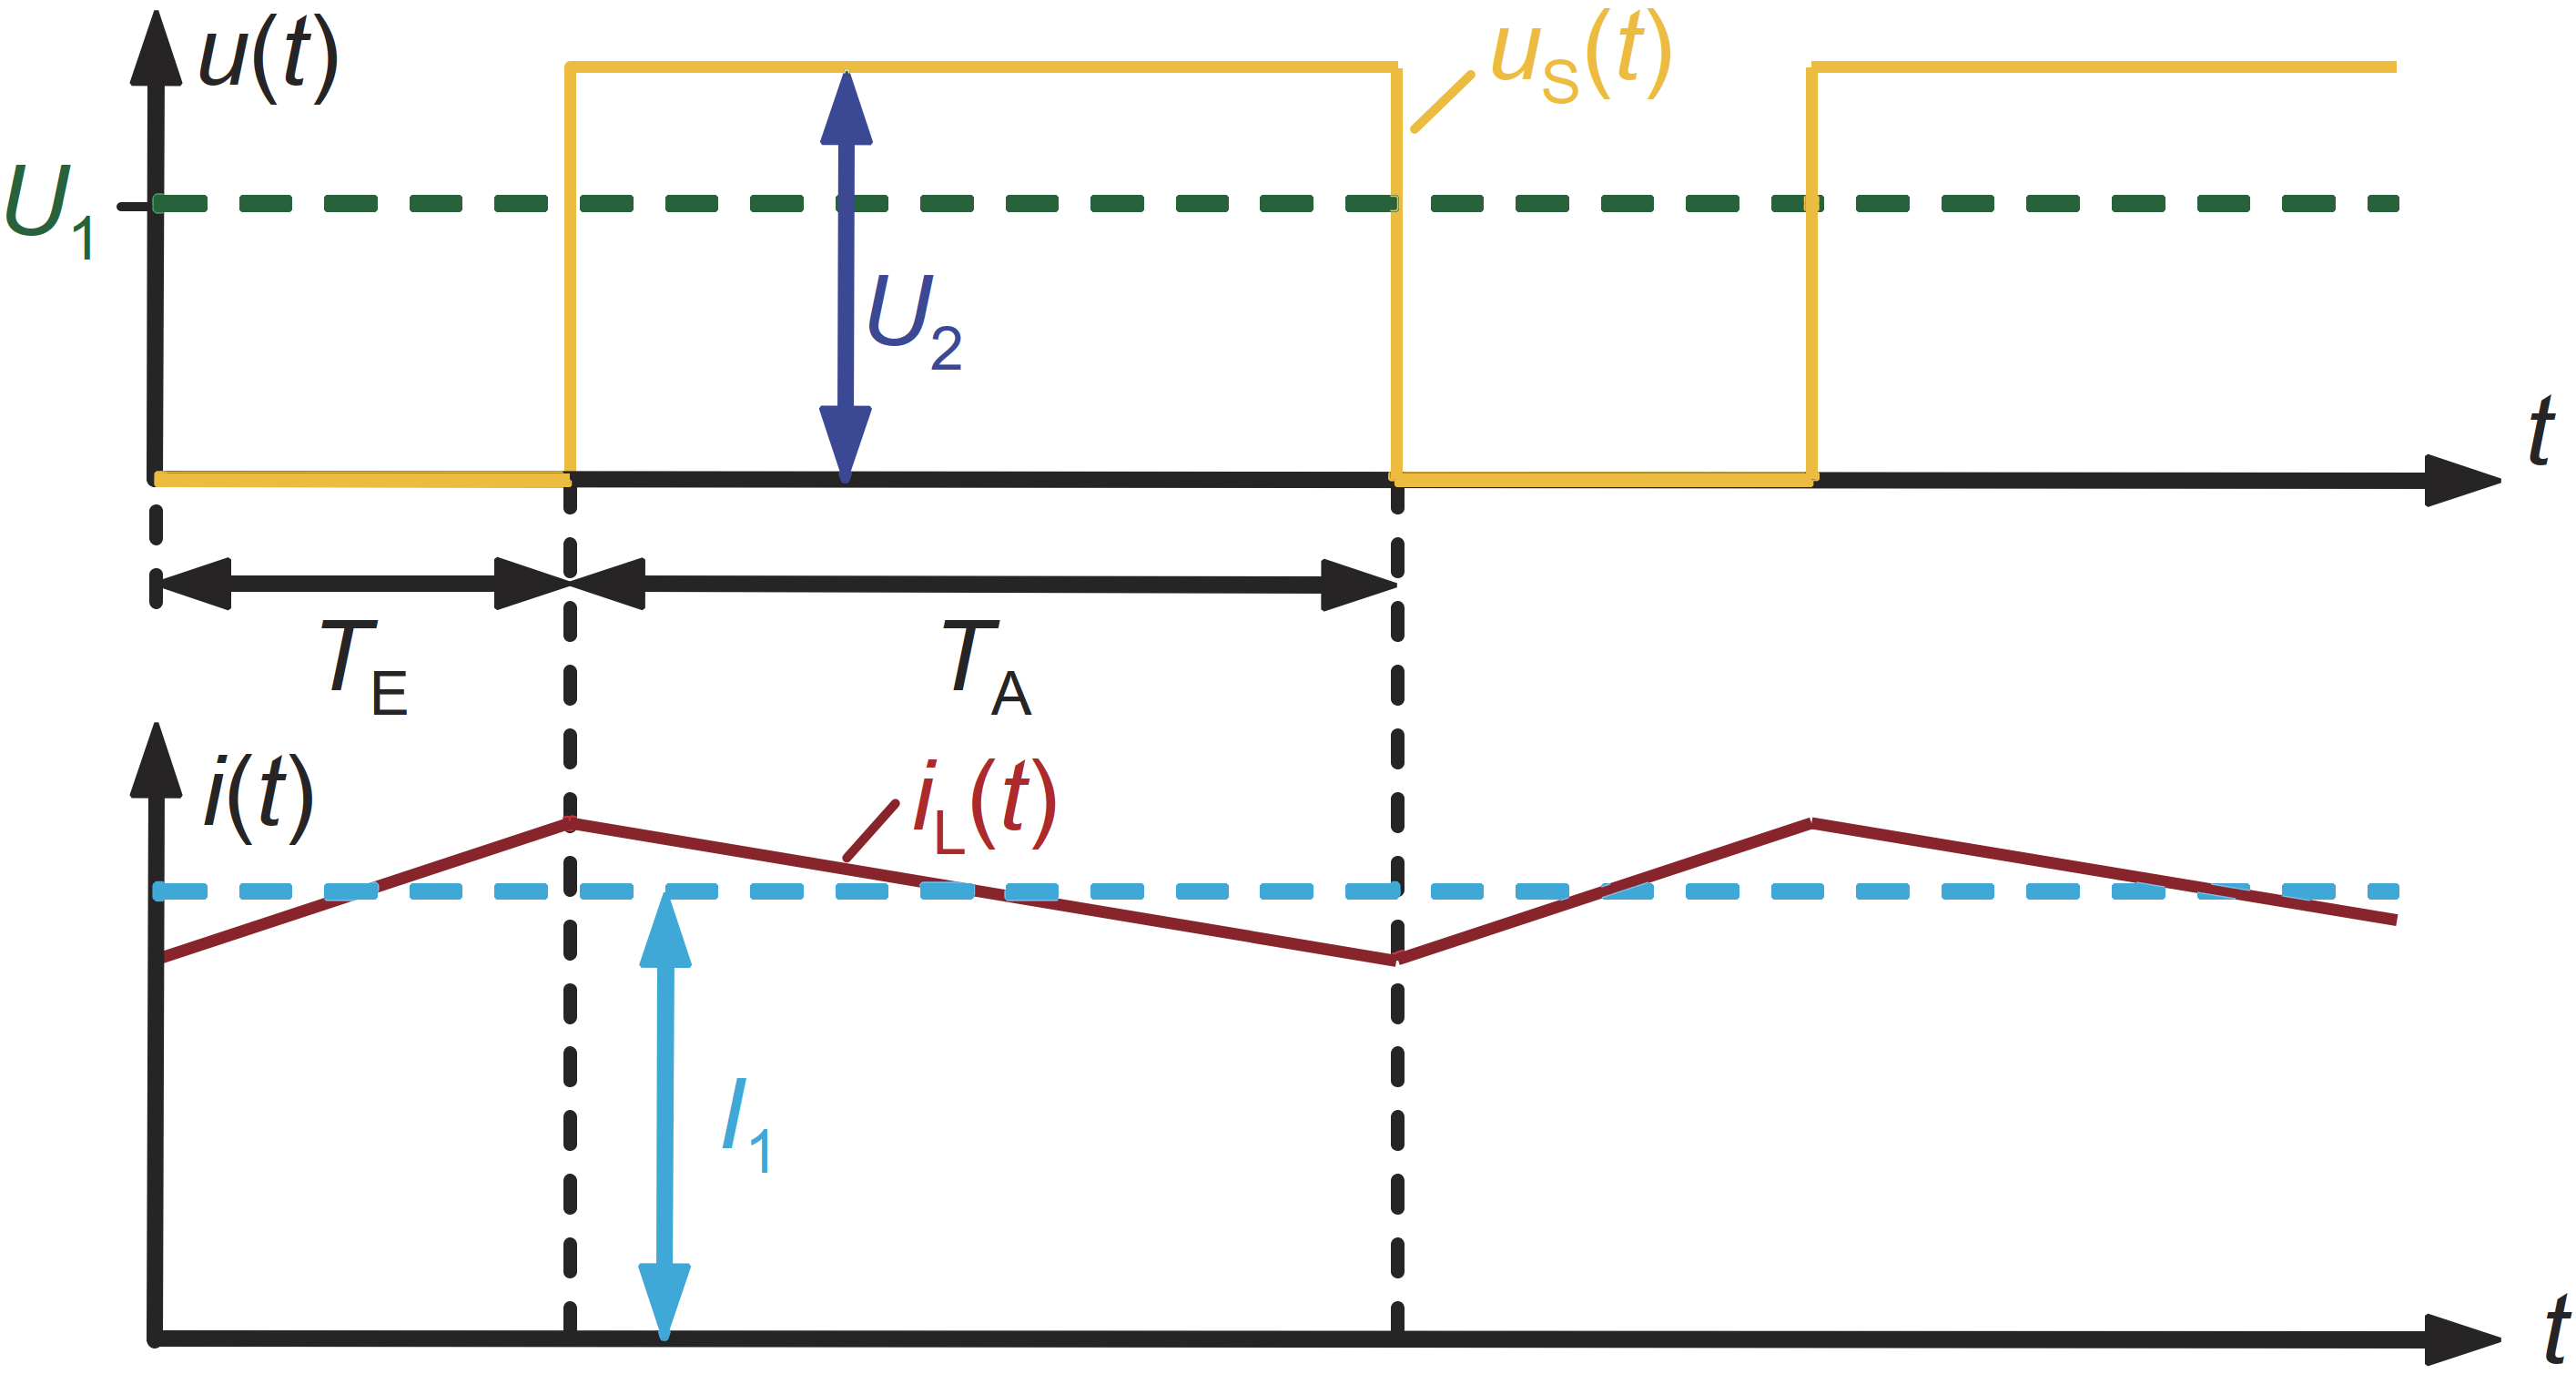
\includegraphics[width=0.8\columnwidth]{images/Hochstellsetzer_2.png}

\vspace{0.25cm}


Nach der Zeitdauer $T_E$ wird der Transistor gesperrt. Die Drossel versucht, ihren Strom aufrecht zu erhalten. Wir nehmen an, dass $U_2 > U_1$ ist. In diesem Fall treibt die Drossel den Strom langsam absinkend über die Diode $D$ auf den Ausgang.

Die Spannung an der Drossel ergibt sich zu:

\begin{minipage}[t]{0.23\columnwidth}
\textbf{\myul{Während $T_E$}}

\end{minipage}
\hfill
\begin{minipage}[c]{0.73\columnwidth}
\textbf{\myul{Während $T_A$}}

\end{minipage}


\begin{minipage}[t]{0.23\columnwidth}

$
\boxed{\frac{\mathrm{d}i_L}{\mathrm{d}t} = \frac{u_L}{L} = \frac{U_1}{L}}
$
\end{minipage}
\hfill
\begin{minipage}[c]{0.73\columnwidth}

$
\boxed{u_L = U_1 - U_2}
$
$
\boxed{\frac{\mathrm{d}i_L}{\mathrm{d}t} = \frac{u_L}{L} = \frac{U_1 - U_2}{L}}
$
\end{minipage}





\subsection{Berechnung der Ausgangsspannung}

Aus der Beziehung zwischen Ein- und Ausgangsspannung ergibt sich zunächst:

$
\boxed{U_2 \cdot T_A = U_1 \cdot T}
$

Daraus folgt für die Ausgangsspannung:

$
\boxed{U_2 = \frac{T}{T_A} \cdot U_1 = \frac{T}{T - T_E} \cdot U_1 = \frac{1}{1 - \frac{T_E}{T}} \cdot U_1 = \frac{1}{1 - a} \cdot U_1}
$



        \columnbreak
\section{Wechselrichter WR}
\subsection{Wirkungsgrade WR}

$
\boxed{
\eta_\text{MPPT} = \frac{P_\text{DC}}{P_\text{MPP}}
}$
$
\boxed{
\eta_\text{Um} = \frac{P_\text{AC}}{P_\text{DC}}
}$
$
\boxed{
\eta_\text{WR} = \eta_\text{MPPT} \cdot \eta_\text{Um}
}$
$
\boxed{
\eta_\text{WR} = \frac{P_\text{AC}}{P_\text{MPP}}
}
$

\vspace{0.1cm}

\begin{minipage}[t]{0.48\columnwidth}
    \renewcommand{\arraystretch}{1.2}
    \begin{tabular}{@{} l p{2.8cm} l @{}}
        $[\eta_\text{MPPT}]$ & Anpassungsw \dotfill & $\mathrm{-}$ \\
        $[\eta_\text{Um}]$   & Umwandlungsw \dotfill   & $\mathrm{-}$ \\
        $[\eta_\text{WR}]$   & Gesamtw \dotfill & $\mathrm{-}$ \\
    \end{tabular}
\end{minipage}
\hfill
\vrule width 1pt
\hfill
\begin{minipage}[t]{0.48\columnwidth}
    \renewcommand{\arraystretch}{1.2}
    \begin{tabular}{@{} l p{2.8cm} l @{}}
        $[P_\text{MPP}]$     & MPP-Leistung \dotfill     & $\mathrm{W}$ \\
        $[P_\text{DC}]$      & Leist. WR-Eingang \dotfill   & $\mathrm{W}$ \\
        $[P_\text{AC}]$      & Leist. WR-Ausgang \dotfill  & $\mathrm{W}$ \\
    \end{tabular}
\end{minipage}

\subsection{Dimmensionierung WR}

Typischer Wert: $SR_{\mathrm{AC}} = 1$, \quad Je nach Standort, AusRtg und Neigung: $ 0.8 \ldots 1.2$

\vspace{0.1cm}

$
\boxed{SR_{\mathrm{AC}} = \frac{P_{\mathrm{STC}}}{P_{\mathrm{AC\_N}}}}
$
$
\boxed{SR_{\mathrm{AC}} = \frac{n \cdot P_{\mathrm{STC,Modul}}}{P_{\mathrm{AC,N}}}}
$
$
\boxed{
n = \frac{SR_{\mathrm{AC}} \cdot P_{\mathrm{AC\_N}}}{P_{\mathrm{STC,Modul}}}
}
$

\vspace{0.1cm}

\renewcommand{\arraystretch}{1.2}
\begin{tabular}{@{} l p{6.5cm} l @{}}
    $[SR_{\mathrm{AC}}]$   & Auslegungsfaktor (Sizing Ratio) \dotfill                        & $-$ \\
    $[P_{\mathrm{STC}}]$   & Summe aller $P_{\mathrm{STC,Modul}}$ (bei STC) \dotfill         & $\mathrm{kW}$ \\
    $[P_{\mathrm{AC\_N}}]$  & Ausgangs-Nennleistung des Wechselrichter \dotfill                   & $\mathrm{kW}$ \\
    $[P_{\mathrm{STC,Modul}}]$   & Modulleistung bei STC \dotfill         & $\mathrm{kW}$ \\
    $[n]$   & Anzahl Module \dotfill                        & $-$ \\
\end{tabular}


\vspace{0.1cm}





\subsection{Spannungsdimensionierung von PV-Strings}

\subsubsection{Maximale Anzahl Module in einem String}

\begin{minipage}[t]{0.48\columnwidth}
\textbf{Aufgrund max zuläss. Spannung:}

$
\boxed{
n_{\mathrm{Max,L}} = \frac{U_{\mathrm{WR,Max}}}{U_{\mathrm{L,Modul \, (-10 \, ^\circ\mathrm{C})}}}
}
$
\end{minipage}
\hfill
\vrule width 1pt
\hfill
\begin{minipage}[t]{0.48\columnwidth}
\textbf{Aufgrund  MPP-Arbeitsbereichs:}

$
\boxed{
n_{\mathrm{Max,MPP}} = \frac{U_{\mathrm{WR,MPP,Max}}}{U_{\mathrm{MPP,Modul \, (-10 \, ^\circ\mathrm{C})}}}
}
$
\end{minipage}

\vspace{0.1cm}



\subsubsection{Minimale Anzahl Module in einem String}

\textbf{Aufgrund des MPP-Arbeitsbereichs:}

$
\boxed{
n_{\mathrm{Min,MPP}} = \frac{U_{\mathrm{WR,MPP,Min}}}{U_{\mathrm{MPP,Modul \, (70 \, ^\circ\mathrm{C})}}}
}
$

\vspace{0.1cm}

\renewcommand{\arraystretch}{1.2}
\begin{tabular}{@{} l p{6.5cm} l @{}}
    $[n_{\mathrm{Max,L}}]$        & Max. Anzahl Module (Spannungsgrenze) \dotfill & $-$ \\
    $[n_{\mathrm{Max,MPP}}]$      & Max. Anzahl Module (MPP-Spannungsbereich) \dotfill & $-$ \\
    $[n_{\mathrm{Min,MPP}}]$      & Min. Anzahl Module (MPP-Spannungsbereich) \dotfill & $-$ \\
    $[U_{\mathrm{WR,Max}}]$       & Max. Eingangsspannung des WR \dotfill & $\mathrm{V}$ \\
    $[U_{\mathrm{WR,MPP,Max}}]$   & Max. MPP-Spannungsbereich WR \dotfill & $\mathrm{V}$ \\
    $[U_{\mathrm{WR,MPP,Min}}]$   & Min. MPP-Spannungsbereich WR \dotfill & $\mathrm{V}$ \\
    $[U_{\mathrm{L,Modul \, (-10 \, ^\circ\mathrm{C})}}]$    & Leerlaufspannung Modul bei $\vartheta_{\mathrm{Zell}} =  -10 \, ^\circ \mathrm{C}$ \dotfill & $\mathrm{V}$ \\
    $[U_{\mathrm{MPP,Modul \, (70 \, ^\circ\mathrm{C})}}]$ & MPP-Spannung pro Modul bei Temperatur $\vartheta_{\mathrm{Zell}} = 70 \, ^\circ\mathrm{C}$ \dotfill & $\mathrm{V}$ \\
\end{tabular}



\subsection{Stromdimensionierung von PV-Strings}

\subsubsection{Maximale Anzahl paralleler Strings}

\begin{minipage}[t]{0.48\columnwidth}
\textbf{Aufgr. max zuläss. Kurzschlussstrom:}

$
\boxed{
n_{\mathrm{String,K}} = \frac{I_{\mathrm{WR,Max}}}{I_{\mathrm{K,Modul \, (70 \, ^\circ\mathrm{C})}}}
}
$
\end{minipage}
\hfill
\vrule width 1pt
\hfill
\begin{minipage}[t]{0.48\columnwidth}
\textbf{Aufgr. max Eingangsstrom:}

$
\boxed{
n_{\mathrm{String,MPP}} = \frac{I_{\mathrm{WR,Eingang,Max}}}{I_{\mathrm{MPP,Modul \, (70 \, ^\circ\mathrm{C})}}}
}
$
\end{minipage}

\vspace{0.1cm}

\renewcommand{\arraystretch}{1.2}
\begin{tabular}{@{} l p{6.5cm} l @{}}
    $[n_{\mathrm{String,K}}]$        & Max. Anzahl paralleler Strings (Kurzschlussgrenze) \dotfill & $-$ \\
    $[n_{\mathrm{String,MPP}}]$      & Max. Anzahl paralleler Strings (Eingangsstromgrenze) \dotfill & $-$ \\
    $[I_{\mathrm{WR,Max}}]$          & Max. PV-Kurzschlussstrom ($\mathrm{I_{SC\_PV}}$) \dotfill & $\mathrm{A}$ \\
    $[I_{\mathrm{WR,Eingang,Max}}]$  & Max. Eingangsstrom ($\mathrm{I_{DCmax}}$)\dotfill & $\mathrm{A}$ \\
    $[I_{\mathrm{K,Modul \, (70 \, ^\circ\mathrm{C})}}]$     & Kurzschlussstrom des Moduls bei $T = 70 \, ^\circ\mathrm{C}$ \dotfill & $\mathrm{A}$ \\
    $[I_{\mathrm{MPP,Modul \, (70 \, ^\circ\mathrm{C})}}]$   & MPP-Strom des Moduls bei $T = 70 \, ^\circ\mathrm{C}$ \dotfill & $\mathrm{A}$ \\
\end{tabular}


\subsection{PV-Netzkopplung}

\begin{tabular}{|l|p{3cm}|p{3.8cm}|}
\hline
\textbf{Aspekt} & \textbf{Früher: netzfolgend} & \textbf{Heute: netzführend}  \\
\hline
Frequenzhaltung & Abschaltung bei f > 50{,}2 Hz und f < 49{,}5 Hz & Kennlinie P(f) bei 50{,}2 bis 51{,}5 Hz  
 \\
\hline
Wirkleistung & Keine Regelung / Volleinspeisung & 
\begin{itemize}
  \item Wirkleistungsbegrenzung (z.\,B. 70\,\%)
  \item Wirkleistungsreduktion auf Anforderung durch Netzbetreiber (Rundsteuersignal)
\end{itemize} \\
\hline
Blindleistung & Cos~$\varphi$ = 1 & Cos~$\varphi$ -0{,}8 bis 0{,}8 (feste Einstellung, Rundsteuersignal, Q(U))  \\
\hline
Immunität & Abschaltung & Immunität gegen Netzstörung (Fault Ride Through)  \\
\hline
\end{tabular}

\vspace{0.1cm}

\textbf{Zukünftig: netzbildend}

\begin{minipage}[t]{0.48\columnwidth}
\begin{itemize}
  \item Systemspannung bilden
  \item Fehlerströme einspeisen
  \item Aktiv Oberwellen filtern
  \item Spannungsasymmetrien ausgleichen
\end{itemize}
\end{minipage}
\hfill
\begin{minipage}[t]{0.48\columnwidth}
\begin{itemize}
  \item Virtuelle Trägheit
  \item Erweitertes Fault Ride Through
  \item Netzstabilisierende Unterstützung
\end{itemize}
\end{minipage}
        \section{Batterien (Akkus)}

\textbf{Elektrochemische Speicher}
\begin{itemize}
    \item Zusammenschaltung mehrerer elektrochemischer Zellen
    \item Jede elektrochemische Zelle besteht aus zwei räumlich getrennten Elektroden, 
          die über einen Elektrolyten als ionenleitende Phase miteinander verbunden sind
    \item An den Elektroden findet eine in zwei Halbreaktionen getrennte Redoxreaktion statt
    \item Energie als im äußeren Stromkreis fließende Elektronen
\end{itemize}

\textbf{Einteilung}
\begin{itemize}
    \item Primär- oder Sekundärzellen
    \item Niedertemperatur-Batterien (z.B. Blei-, Nickel- und Lithium-Batterien)
    \item Hochtemperatur-Batterien (z.B. Natrium-Batterien)
    \item Interner oder externer Speicher (z.B. Redox-Flow-Batterien)
\end{itemize}

\subsection{Nennkapazität $C_{\text{nenn}}$}

\begin{minipage}[t]{0.23\columnwidth}
$
\boxed{C_{\text{nenn}} = \frac{C_{\text{nutzbar}}}{\mathrm{DOD_{Zul}}}}
$
\end{minipage}
\hfill
\begin{minipage}[t]{0.73\columnwidth}
    \renewcommand{\arraystretch}{1.2}
        \begin{tabular}{@{} l p{4.5cm} l @{}}
            $[C_{\text{nenn}}]$     & Nennkapazität der Batterie \dotfill          & $\mathrm{kWh}$ \\
            $[C_{\text{nutzbar}}]$  & Nutzbare Kapazität \dotfill                  & $\mathrm{kWh}$ \\
            $[\mathrm{DOD_{Zul}}]$          & Zulässige Entladetiefe \dotfill   & $-$ \\
\end{tabular}
\end{minipage}



\subsection{Vollzyklen $N_{\text{voll}}$}

\begin{minipage}[t]{0.25\columnwidth}
$
\boxed{N_{\text{voll}} = N_{\text{teil}} \cdot \mathrm{DOD_{Entl}}}
$
\end{minipage}
\hfill
\begin{minipage}[t]{0.71\columnwidth}
    \renewcommand{\arraystretch}{1.2}
        \begin{tabular}{@{} l p{4.5cm} l @{}}
            $[N_{\text{voll}}]$  & Anzahl geleisteter Vollzyklen \dotfill          & $-$ \\
            $[N_{\text{teil}}]$  & Anzahl Teilzyklen \dotfill                        & $-$ \\
            $[\mathrm{DOD_{Entl}}]$       & Entladetiefe (entnommen) \dotfill & $-$ \\
    \end{tabular}
\end{minipage}


\subsection{Gesundheitszustand der Batterie (SOH)}

\begin{minipage}[t]{0.32\columnwidth}
$
\boxed{\text{SOH} = 1 - \frac{N_{\text{voll}}}{N_{\text{zykl}}}\cdot (1 - \text{EOL})}
$
\end{minipage}
\hfill
\begin{minipage}[c]{0.58\columnwidth}
    Definition EOL bei 80 \% der Nennkapazität $C_{\mathrm{nenn}}$ (EN 60896) (normalerweise EOL = 0.8)
\end{minipage}

\vspace{0.1cm}

\begin{minipage}[t]{0.48\columnwidth}
    \renewcommand{\arraystretch}{1.2}
    \begin{tabular}{@{} l p{2.8cm} l @{}}
        $[\text{SOH}]$        & State of Health     \dotfill    & $\mathrm{\%}$ \\
        $[N_{\text{voll}}]$   & Geleistete Vollzyklen               \dotfill              & $-$ \\
    \end{tabular}
\end{minipage}
\hfill
\vrule width 1pt
\hfill
\begin{minipage}[t]{0.48\columnwidth}
    \renewcommand{\arraystretch}{1.2}
    \begin{tabular}{@{} l p{2.8cm} l @{}}
        $[N_{\text{zykl}}]$   & Zyklenfestigkeit                    \dotfill                   & $-$ \\
        $[\text{EOL}]$        & End-of-Life                  \dotfill & $-$ \\
    \end{tabular}
\end{minipage}



\subsection{Ladezustand (SOC)}

\begin{minipage}[t]{0.23\columnwidth}
$
\boxed{\text{SOC} = \frac{\sum P_i \cdot t_i}{C_{\text{nutzbar}}}}
$
\end{minipage}
\hfill
\begin{minipage}[t]{0.73\columnwidth}
    \renewcommand{\arraystretch}{1.2}
\begin{tabular}{@{} l p{4.5cm} l @{}}
    $[\text{SOC}]$         & Ladezustand der  Batterie \dotfill           & $\mathrm{\%}$ \\
    $[P_i]$                & Ladeleistung $i$ \dotfill      & $\mathrm{kW}$ \\
    $[t_i]$                 & Ladedauer Intervall $i$ \dotfill       & $\mathrm{h}$ \\
    $[C_{\text{nutzbar}}]$    & Nutzbare Kapazität \dotfill                 & $\mathrm{kWh}$ \\
\end{tabular}
\end{minipage}



\subsection{C-Rate}

\begin{minipage}[t]{0.23\columnwidth}
$
\boxed{C\text{-Rate} = \frac{P_{\text{Lade}}}{C_{\text{nenn}}}}
$
\end{minipage}
\hfill
\begin{minipage}[t]{0.73\columnwidth}
    \renewcommand{\arraystretch}{1.2}
\begin{tabular}{@{} l p{4.5cm} l @{}}
    $[C\text{-Rate}]$      & Verhältnis Ladeleistung zu Kapazität \dotfill & $\mathrm{1/h}$ \\
    $[P_{\text{Lade}}]$    & Ladeleistung \dotfill                         & $\mathrm{kW}$ \\
    $[C_{\text{nenn}}]$    & Nennkapazität der Batterie \dotfill           & $\mathrm{kWh}$ \\
\end{tabular}
\end{minipage}



\subsection{Lithium-Ionen-Batterien}

\subsubsection{Aufbau}

\begin{enumerate}
  \item Stromableiter
  \begin{itemize}
    \item Aluminium an der positiven Elektrode
    \item Kupfer an der negativen Elektrode
  \end{itemize}
  
  \item Positive Elektrode (Kathode, z.\,B. LiCoO\textsubscript{2})
  \begin{itemize}
    \item Metallische Struktur mit \glqq variablem\grqq{} Anteil an Li\textsuperscript{+}-Ionen
  \end{itemize}
  
  \item Negative Elektrode (Anode, z.\,B. Graphit/C\textsubscript{6})
  
  \item Separator (PP oder PE)
  \begin{itemize}
    \item Mikro-poröser Kunststoff, ionendurchlässig
  \end{itemize}
  
  \item Elektrolyt (z.\,B. LiPF\textsubscript{6})
  \begin{itemize}
    \item Ionenleiter (elektrisch nicht leitend)
  \end{itemize}
\end{enumerate}



\subsubsection{Aktivmaterialien}

\begin{minipage}[t]{0.6\columnwidth}
\textbf{Positive Elektrode:}
  \begin{itemize}
    \item Lithiumeisenphosphat (LFP)
    \item Lithium-Nickel-Mangan-Kobaltoxid (NMC)
    \item Lithiumkobaltoxid (LCO)
    \item Lithiummanganoxid (LMO)
    \item Lithium-Nickel-Kobalt-Aluminiumoxid (NCA)
  \end{itemize}
\end{minipage}
\hfill
\begin{minipage}[t]{0.36\columnwidth}
\textbf{Negative Elektrode:}
  \begin{itemize}
    \item Graphit (C\textsubscript{6})
    \item Lithiumtitanat (LTO)
  \end{itemize}
\end{minipage}



\subsubsection{Bauformen}

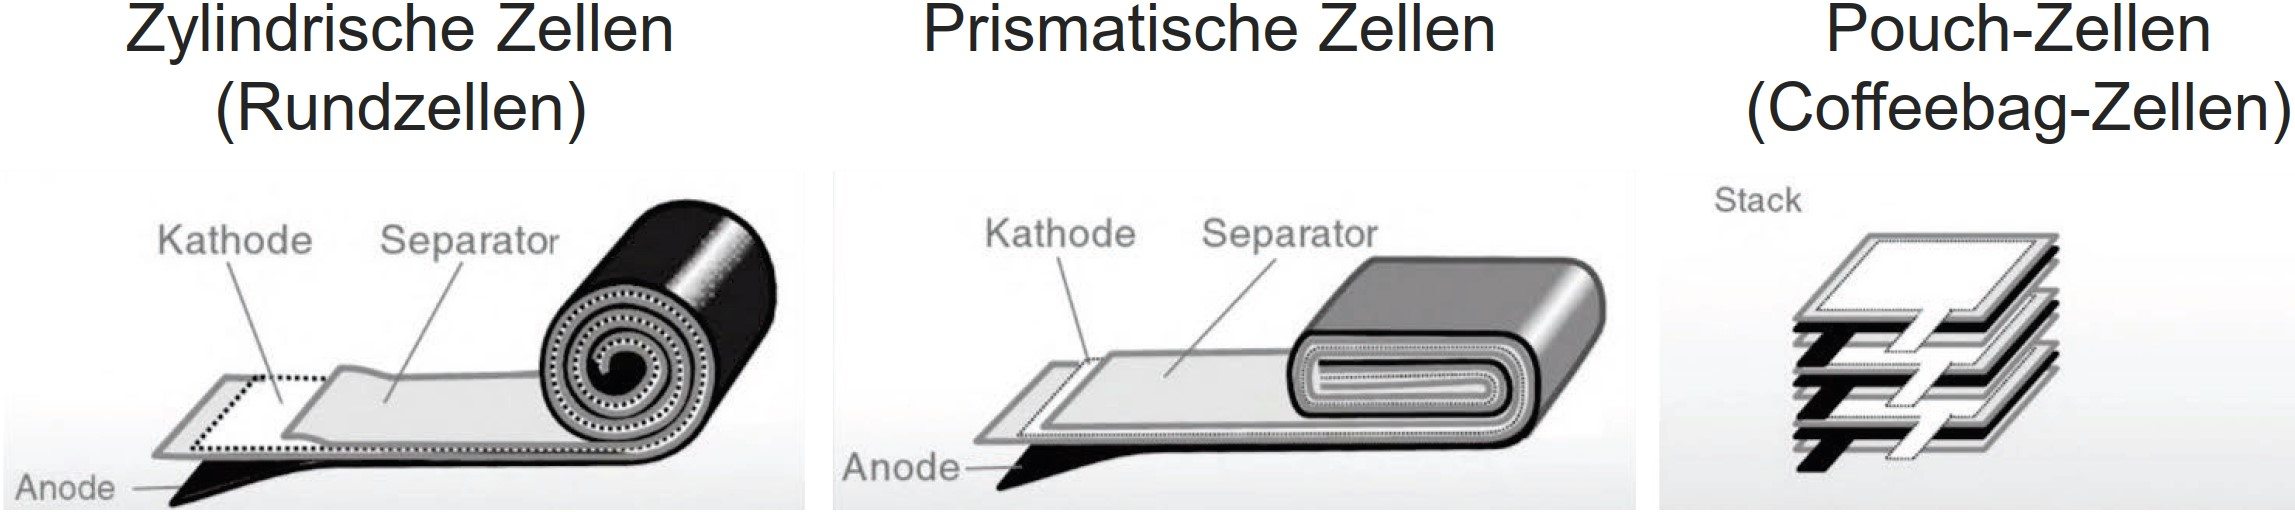
\includegraphics[width=0.98\columnwidth]{images/Aufbau_Batterie_1.jpg}


\columnbreak
\subsubsection{Ladeverfahren}

Typisch: I/U-Laden bzw. CCCV-Verfahren (Constant Current/Constant Voltage)\\
\begin{center}
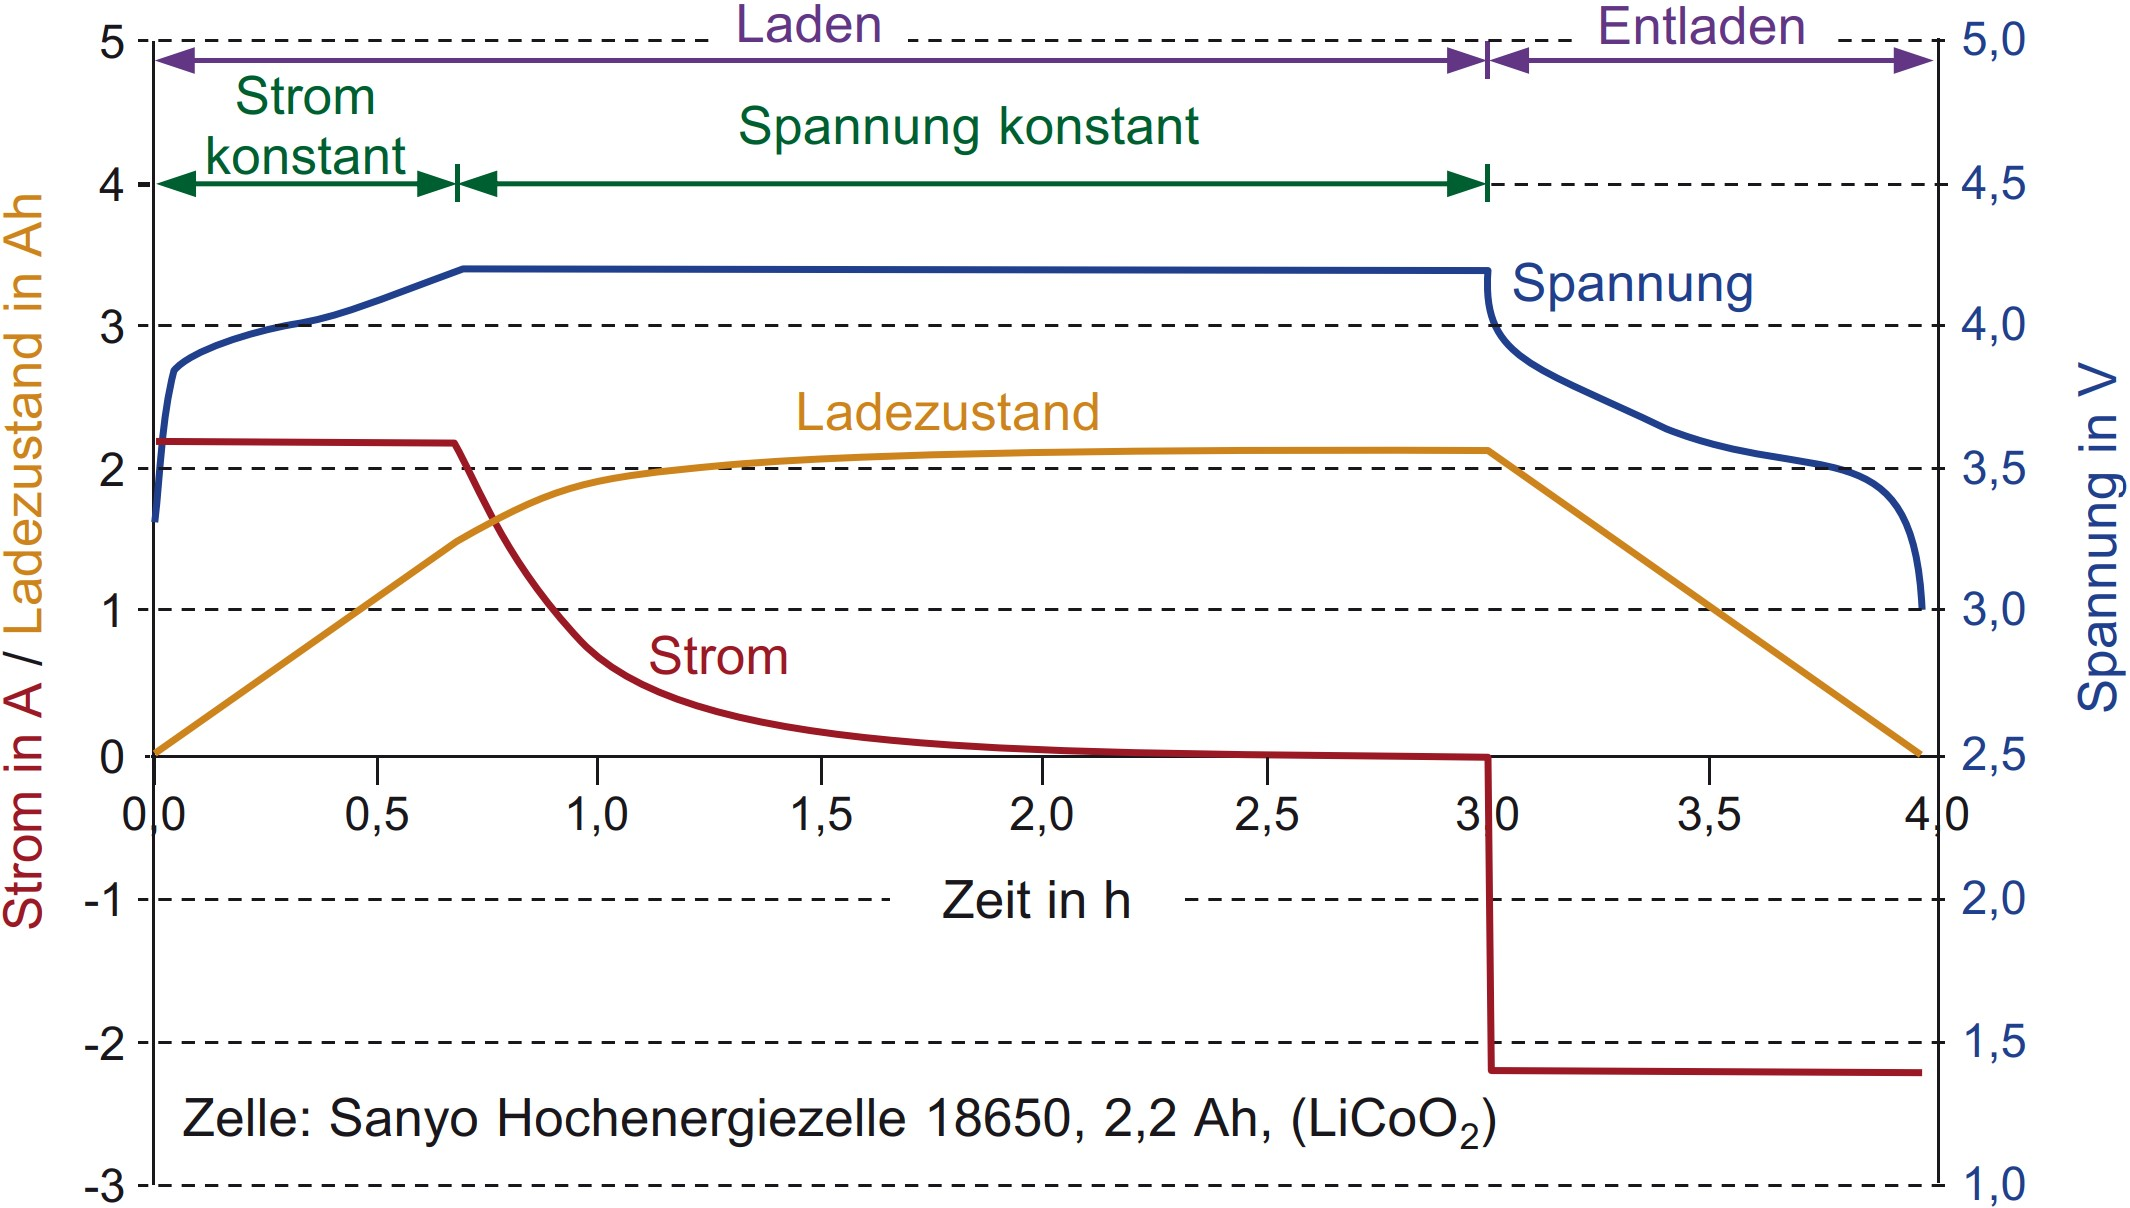
\includegraphics[width=0.8\columnwidth]{images/Lithium_Ionen_Akku.jpg}
\end{center}

Typisch ist eine Ladung nach dem CCCV-Verfahren (Constant Current / Constant Voltage) oder auch I/U-Ladung genannt. Dabei wird die Batterie zunächst mit einem konstanten Strom geladen. Sobald die Ladeschlussspannung erreicht ist, wird auf eine konstante Ladespannung umgeschaltet, um die Batterie vollständig aufzuladen aber nicht zu überladen.




\subsubsection{Kapazität}
Unter anderem abhängig von Entladestrom und Temperatur



\subsubsection{Alterung}


\begin{minipage}[t]{0.48\columnwidth}
\textbf{Kalendarische Alterung}
  \begin{itemize}
    \item Temperatur
    \item Ladezustand
  \end{itemize}
\end{minipage}
\hfill
\begin{minipage}[t]{0.48\columnwidth}
\textbf{Zyklenfestigkeit}
  \begin{itemize}
    \item Lade- und Entladerate
    \item Temperatur
    \item Ladezustand
    \item Entladetiefe
  \end{itemize}
\end{minipage}



\subsubsection{Vor- und Nachteile}

\begin{minipage}{0.48\textwidth}
\textbf{Vorteile}
\begin{itemize}
  \item Höchste Energiedichte und Wirkungsgrade
  \item Hohe Leistungsfähigkeit
  \item Keine spez. Standortanforderungen
  \item Schnellladefähigkeit
  \item Sehr geringe Selbstentladung (< 3\,\% pro Jahr bei Raumtemperatur, bis 15\,\% bei hohen Temperaturen)
  \item Grosses Anwendungsspektrum im stationären und mobilen Bereich
  \item Grosse Stückzahlen führen zu Kostensenkung
  \item Grösster Hoffnungsträger, höchste Forschungs- und Entwicklungstätigkeit
  \item Entwicklung neuer Aktivmaterialien
\end{itemize}
\end{minipage}
\hfill
\begin{minipage}{0.48\textwidth}
\textbf{Nachteile}
\begin{itemize}
  \item Keine inhärente Sicherheit (thermisches Durchgehen)
  \item Aufwändiges Batteriemanagementsystem für Sicherheit und Lebensdauer, Einzelzellüberwachung
  \item Lebensdauer begrenzt bei Ladezuständen ausserhalb 30--70\,\%
  \item Entnehmbare Kapazität sinkt bei tiefen Temperaturen
  \item Herstellung (Packaging) und Kühlung aufwendig
  \item (Noch) hohe Kosten
  \item Umweltverträglichkeit beim Lithiumabbau, soziale Akzeptanzprobleme
  \item Begrenzte Vorkommen an Lithium und weiteren Rohstoffen
\end{itemize}
\end{minipage}


\columnbreak
\subsection{Bleibatterie}
\subsubsection{Typen}

\begin{itemize}
  \item Pufferbetrieb (Autobatterie) vs. Zyklenbetrieb (Solarbatterie)

  \item Typische Solarbatterien
  \begin{itemize}
    \item Unterscheidung nach Elektrolyt
    \begin{itemize}
      \item \textbf{Blei-Säure-Batterie}
      \begin{itemize}
        \item Raumbelüftung (Gasung)
        \item Nachfüllen von Wasser
      \end{itemize}

      \item \textbf{Blei-Gel-Batterie}
      \begin{itemize}
        \item Elektrolyt durch Zusätze zu einem Gel verdickt $\rightarrow$ auslaufsicher
        \item Kein Gasaustritt $\rightarrow$ kein Nachfüllen von Wasser
        \item Wichtig: Einhaltung der Ladeschlussspannung (sonst Gasung)
      \end{itemize}
    \end{itemize}
    \item Unterscheidung nach Aufbau der Elektroden
        \begin{itemize}
        \item Blockbatterien (Blockakkus) mit mehreren Bleistäben von einer gemeinsamen Schutzhülle umgeben
        \item ortsfeste Panzerplattenbatterien, bei denen jeder Bleistab von einer Schutzhülle umgeben ist
      \end{itemize}
  \end{itemize}
\end{itemize}



\subsubsection{Vor- und Nachteile}

\begin{minipage}[t]{0.48\textwidth}
\textbf{Vorteile}
\begin{itemize}
  \item Etablierteste Batterietechnologie, weltweit lange Erfahrungen, seit 150 Jahren im Einsatz
  \item Relativ kostengünstiges Batteriesystem
  \item Akzeptable Energie- und Leistungsdichte für stationäre Anwendungen
  \item Hohe Sicherheit im Vergleich zu Lithium- oder Natrium-Batterien
  \item Kein komplexes Zellmanagement erforderlich
  \item Vollladung unschädlich
  \item Unabhängig von Standortbedingungen
  \item Vollautomatisierte Massenproduktion ermöglicht Kostensenkung
  \item Viele Hersteller weltweit
  \item Günstigster Speicher für Inselnetze
\end{itemize}
\end{minipage}
\hfill
\begin{minipage}[t]{0.48\textwidth}
\textbf{Nachteile}
\begin{itemize}
  \item Schädliche Tiefentladungen
  \item Lange Standzeiten mit tiefen Ladezuständen vermeiden
  \item Gutes Temperaturmanagement erforderlich
  \item Batterieraumbelüftung erforderlich (Blei-Säure)
  \item Lade- und Entladefähigkeit nicht symmetrisch
  \item Begrenzte Zyklenlebensdauer
  \item Konkurrenz durch Kostensenkung bei Lithium-Batterien
  \item Begrenzte Bleilagerstätten
  \item Umweltverträglichkeit
\end{itemize}
\end{minipage}

\vspace{0.1cm}

\textbf{Vorteile gegenüber Lithium-Ionen-Batterien}

\begin{enumerate}
    \item Bleibatterien haben eine hohe Sicherheit (kein thermisches Durchgehen), weshalb auch kein komplexes Zellmanagement notwendig ist. Sie können eher an entlegenen Standorten unbeaufsichtigt gelassen werden.
    \item Eine Vollladung ist unschädlich. In netzfernen Anwendungen wird häufig über eine längere Zeit kein Verbraucher betrieben, es soll aber nach Möglichkeit jederzeit die volle Batteriekapazität zur Verfügung stehen.
\end{enumerate}



\subsection{Nickel-Batterie}


  \textbf{Nickel-Batterien}
  \begin{itemize}
    \item Entwickelt für höhere Energiedichte und Robustheit als Blei
    \item Diverse Typen, in der praktischen Anwendung dominieren:
  \end{itemize}

  \textbf{Nickel-Cadmium (NiCd)}
  \begin{itemize}
    \item Cadmium giftig, daher sinkt die Verwendung, teils verboten
    \item \glqq Memory\grqq-Effekt
    \item Anwendung bei sicherheitskritischen Anwendungen
  \end{itemize}

  \textbf{Nickel-Metall-Hydrid (NiMH)}
  \begin{itemize}
    \item Für Anwendungen im Hochleistungsbereich entwickelt
    \item Etwa doppelte Energiedichte gegenüber NiCd, Leistungsdichte ebenfalls wesentlich höher
    \item Geringerer maximaler Lade- und Entladestrom, kleinerer Temperaturbereich als NiCd, empfindlich gegen Überladung, Überhitzung, falsche Polung, Tiefentladung
    \item Anwendung in Consumerelektronik und Hybridfahrzeugen
  \end{itemize}



\subsubsection{Vor- und Nachteile Nickel-Batterie}

\begin{minipage}{0.48\textwidth}
\textbf{Vorteile}
\begin{itemize}
  \item Einsatz bei tiefen Temperaturen und extremen Umgebungsbedingungen möglich
  \item Tolerant gegenüber Tiefentladung und unterschiedlichen Ladezuständen, können tiefentladen und in jedem Ladezustand gelagert werden
  \item Hohe zyklische und kalendarische Lebensdauer
  \item Hohe Energiedichte
  \item Einsatz im Hochleistungsbereich
\end{itemize}
\end{minipage}
\hfill
\begin{minipage}{0.48\textwidth}
\textbf{Nachteile}
\begin{itemize}
  \item Hohe Kosten für Nickel
  \item Konkurrenz durch Kostensenkung bei Lithium-Batterien
  \item Giftiges Cadmium (bei NiCd)
\end{itemize}
\end{minipage}


\columnbreak
\subsection{Natrium-Batterie}


\textbf{Natrium-Hochtemperatur-Batterien}
  \begin{itemize}
    \item Wärmeisolierter Behälter mit Heizung und Kühlung, BMS erforderlich
    \item Geringe elektrochemische Selbstentladung, aber hohe \glqq thermische Selbstentladung\grqq
  \end{itemize}

\textbf{Natrium-Schwefel-Batterien}
  \begin{itemize}
    \item Betriebstemperatur: 300--350\,\textdegree C
    \item Hohe Zyklenzahl, abhängig von Entladetiefe
    \item Tiefentladung schädlich, verkürzt Lebensdauer, wird i.\,d.\,R. durch BMS vermieden
    \item Hoher Wirkungsgrad, aber thermische Verluste durch Heizung
    \item Betriebssicherheit: Bei Unfällen können durch Reaktionen Temperaturen über 1'000\,\textdegree C entstehen
    \item Anwendung: Grössere stationäre Anwendungen, z.\,B. für Regelenergie
    \end{itemize}

\textbf{Natrium-Nickelchlorid-Batterie (Salzschmelzbatterie, Zebra-Batterie)}
  \begin{itemize}
    \item Betriebstemperatur: 250--350\,\textdegree C
    \item Umweltfreundlich, keine seltenen Materialien (Kochsalz, Nickel, Eisen, Keramik)
    \item Abgekühlt praktisch unbegrenzt lagerfähig, keine Selbstentladung
    \item Grosser Temperaturbereich: $-20$ bis $+60\,^\circ$C
    \item Anwendung: Mobilfunk-Basisstationen, mittelgrosse stationäre Anwendungen, Elektromobilität, Waffensysteme
  \end{itemize}

\textbf{Salzwasserbatterie (wässrige Natrium-Ionen-Batterie)}
  \begin{itemize}
    \item Niedertemperaturbatterie
    \item Geringe Spannung und dadurch niedrige Energiedichte (volumetrisch)
    \item Entnehmbare Kapazität stark abhängig von Entladestromstärke, daher C-Raten bis max. 0{,}25 empfohlen
    \item Anwendung: Heim- und Gewerbespeicher
  \end{itemize}



\subsubsection{Vor- und Nachteile Natrium-Batterie}

\begin{minipage}{0.48\textwidth}
\textbf{Vorteile}
\begin{itemize}
  \item Günstige Rohstoffe
  \item Wenig Einschränkung in Verfügbarkeit der Rohstoffe
  \item Sehr gute Umweltverträglichkeit
  \item Keine lokalen Voraussetzungen, kein Gefahrgut
  \item Hohe Zyklen-, lange kalendarische Lebensdauer
  \item Viele bestehende stationäre Anlagen
  \item Viele auslaufende Patente, neue Hersteller
  \item Hochtemperatur: Hohe Energiedichte
  \item Salzwasser-/Salzschmelze: nicht brennbar, nicht explosiv
  \item Salzwasser: tiefentladefest
\end{itemize}
\end{minipage}
\hfill
\begin{minipage}{0.48\textwidth}
\vspace{0.1cm}
\textbf{Nachteile}
\begin{itemize}
  \item Salzwasser: geringe Energiedichte und Entladeleistung
  \item Hochtemperatur-Batterien:
  \begin{itemize}
    \item Hoher Aufwand für Heizung und Kühlung
    \item Thermische Verluste
    \item Hohe Selbstentladung bei längeren Stillstandszeiten
    \item Gefahrenpotenzial aufgrund hoher Betriebstemperatur
  \end{itemize}
  \item NaS: Sicherheitsprobleme (Brand)
  \item Isolation von Natrium gegenüber Umwelteinflüssen (v.\,a. Wasser)
  \item Nur wenige Hersteller
  \item Konkurrenz zu Blei-Säure- und Li-Ion-Batterien
\end{itemize}
\end{minipage}



\subsection{Redox-Flow-Batterie}

\begin{itemize}
  \item Die Elektrolyte zirkulieren in zwei getrennten Kreisläufen, verbunden nur durch eine ionenleitende Membran
  \item Externer Speicher: unabhängige Dimensionierung von Leistung und Energie
  \begin{itemize}
    \item Schnelle \glqq Ladbarkeit\grqq{} durch Austausch der Elektrolyten
  \end{itemize}
  \item Betriebstemperatur: 20--30\,\textdegree C, über 40\,\textdegree C gefährlich
  \begin{itemize}
    \item BMS notwendig zur Steuerung von Temperatur, Spannung und Strom für optimalen Betriebspunkt
  \end{itemize}
  \item Wirkungsgrad der Zelle ca. 90\,\%, durch Peripheriegeräte (z.\,B. Pumpen) sinkt Systemwirkungsgrad auf 70--80\,\%
  \item Gute Vermeidbarkeit von Selbstentladung, da Elektrolytflüssigkeiten getrennt sind
  \item Anwendung:
  \begin{itemize}
    \item Große Speicherkapazitäten
    \item Lastspitzenausgleich und Spannungsstützung
    \item Bereitstellung von Regel- und Ausgleichsenergie
    \item Backup-/USV-Systeme zur Notstromversorgung
    \item Potenziell: Inselnetze, Elektromobilität
  \end{itemize}
\end{itemize}



\subsubsection{Vor- und Nachteile Redox-Flow-Batterie}

\begin{minipage}{0.48\textwidth}
\textbf{Vorteile}
\begin{itemize}
  \item Energie und Leistung unabhängig skalierbar
  \item Räumliche Trennung von Speicherbehälter und Reaktionszelle
  \item Hohe Zyklenlebensdauer, tiefentladefähig
  \item Lade- und Entladestrategien nicht so wichtig (im Vergleich zu Blei oder Lithium)
  \item Geringer Wartungsaufwand
  \item Einsatz unterschiedlicher Redoxpaare, neue Materialkombinationen, kein Ressourcenengpass
  \item Materialverbesserungen ermöglichen Wirkungsgradsteigerung und Kostensenkung; wirtschaftlich vorteilhaft bei hohem Verhältnis von Kapazität zu Leistung
  \item Viele auslaufende Patente, steigender Wettbewerbsdruck
  \item Standorte unbeschränkt
  \item Gute Umweltverträglichkeit
\end{itemize}
\end{minipage}
\hfill
\begin{minipage}{0.48\textwidth}
\textbf{Nachteile}
\begin{itemize}
  \item Geringe Energie- und Leistungsdichte
  \item Säurehaltige Flüssigkeiten verursachen Leckagen
  \item Teure Speichermedien
  \item Wartungsaufwand für Pumpen
  \item Stromverbrauch der Pumpen
  \item Rechtliche Probleme bei Genehmigung durch große Säuremengen
\end{itemize}
\end{minipage}





\subsection{Übersicht Batterien}

\begin{tabular}{|l|c|c|c|c|}
\hline
\textbf{Eigenschaft} & \textbf{Blei} & \textbf{Li-Ionen} & \textbf{Salzschm.} & \textbf{Salzwasser} \\
\hline
Lebensdauer [Jahre] & 5--15 & 10--20 & >15 & ca. 15 \\
\hline
Zyklenfest. [Zyklen] & 500--3'000 & 3'000--10'000 & 4'500 & >5'000 \\
\hline
Entladetiefe [\%] & 50--70 & 90--95 & ca. 85 & 70--100 \\
\hline
Energiedichte $[\frac{\mathrm{Wh}}{\mathrm{kg}}]$ & 30--40 & 200--250 & 100--120 & ca. 40 \\
\hline
Selbstentl. & 3--5 $\frac{\%}{\mathrm{Monat}}$ & 3--5 $\frac{\%}{\mathrm{Jahr}}$ & 20 $\frac{\%}{\mathrm{Tag}}$ \textcolor{green}{Stb} & Gering \\
\hline
Wirkungsgrad [\%] & 75--85 & 90--98 & 85--95 & 80--90 \\
\hline
Betriebstemp. [\textdegree C] & -10 bis 40 & -5 bis 40 & -20 bis 60 & -5 bis 50 \\
\hline
Max. C-Rate [C] & 0.3--0.5 & 1--3 & \textcolor{red}{(E) $\frac{1}{2}$}, \textcolor{blue}{(L) $\frac{1}{4}$} & 0.25 \\
\hline
(1) $[\frac{\mathrm{CHF}}{\mathrm{kWh}}]$ & 100--300 & 500--1'000 & 550--1'000 & 800--1'200 \\
\hline
(2) $[\frac{\mathrm{CHF}}{\mathrm{kWh}}]$ & 170--500 & 540--1'080 & 650--1'300 & 940--1'400 \\
\hline
\end{tabular}

\vspace{0.1cm}

\textcolor{green}{Stb = Standby}, \textcolor{red}{E = Entladen}, \textcolor{blue}{L = Laden}, Salzschm. = Salzschmelze

(1) = Kosten bezogen auf Nennkapazität $C_{\mathrm{nenn}}$

(2) = Kosten bezogen auf nutzbare Kapazität $C_{\mathrm{nutz}}$























        














\section{Montagesystem}
%\begin{comment}
    

\subsection{Befestigung am Gebäude}
\subsubsection{Dachhaken}
Für Ziegeldächer\\
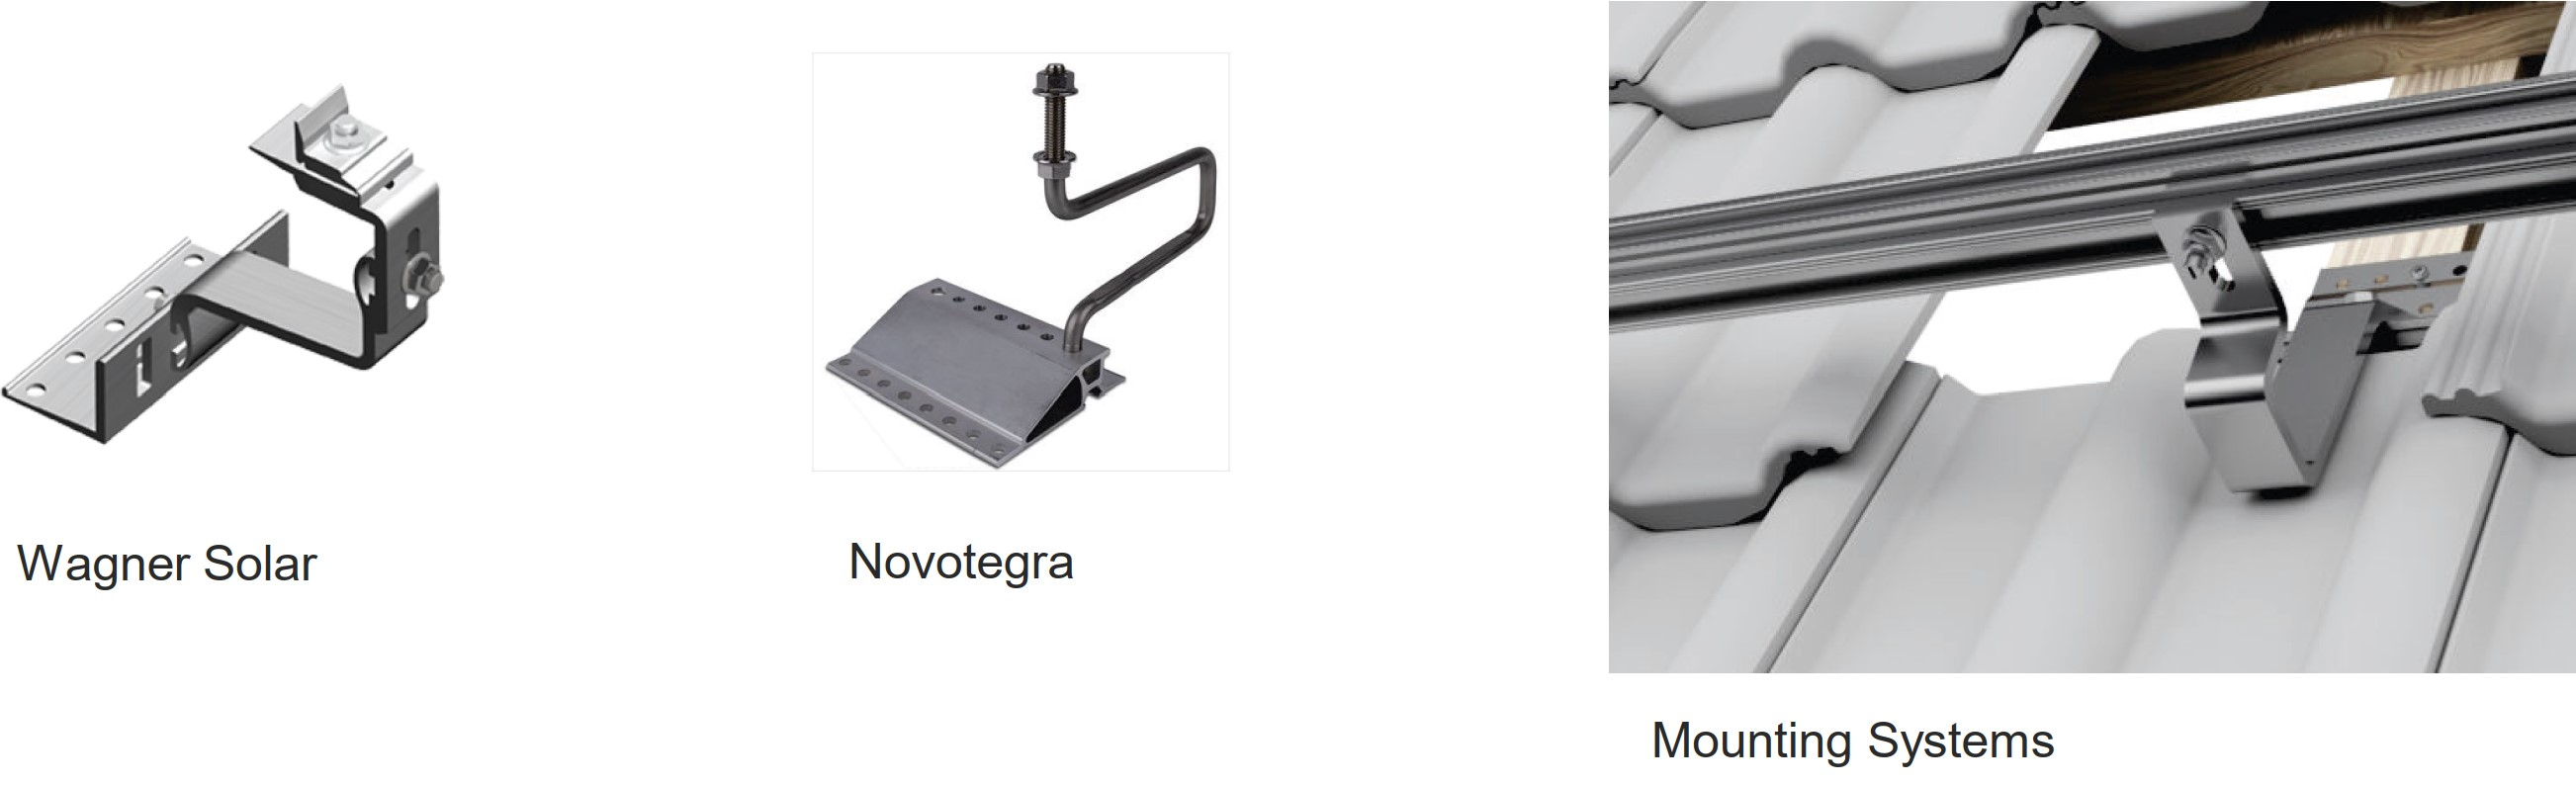
\includegraphics[width=0.95\columnwidth]{images/Dachhaken.jpg}


\subsubsection{Stockschrauben}
Für Well- und Trapezblech-, Faserzement- und Sandwichdächer\\
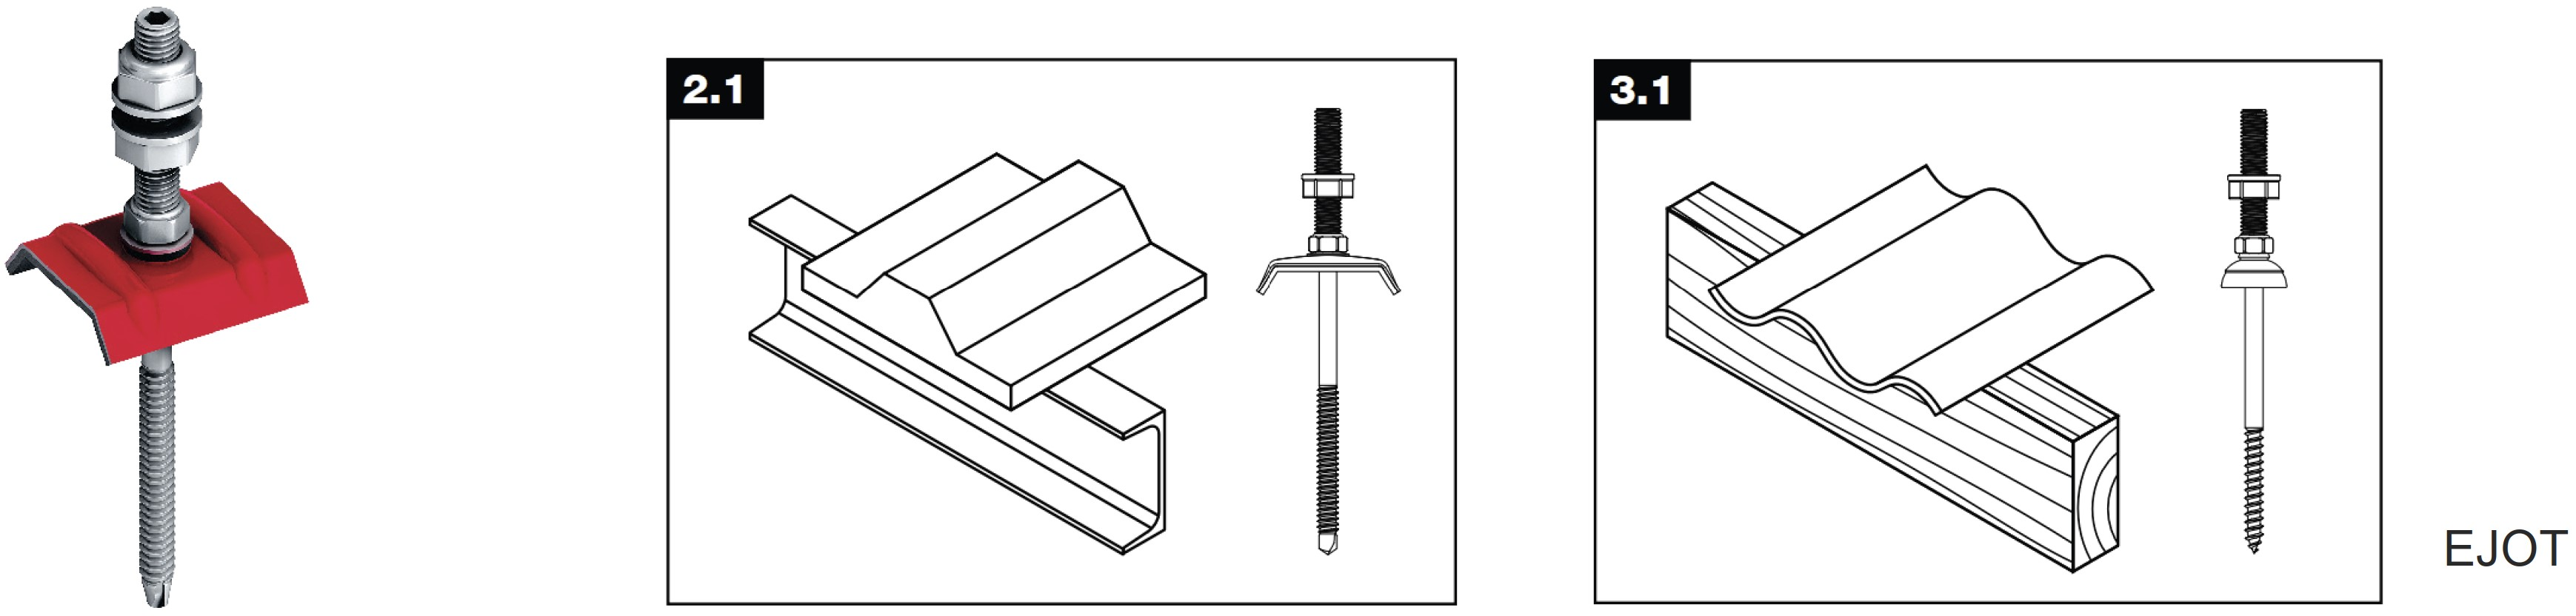
\includegraphics[width=0.95\columnwidth]{images/Stockschrauben.jpg}


\subsubsection{Stehfalzklemmen}
Für Stehfalzdächer\\
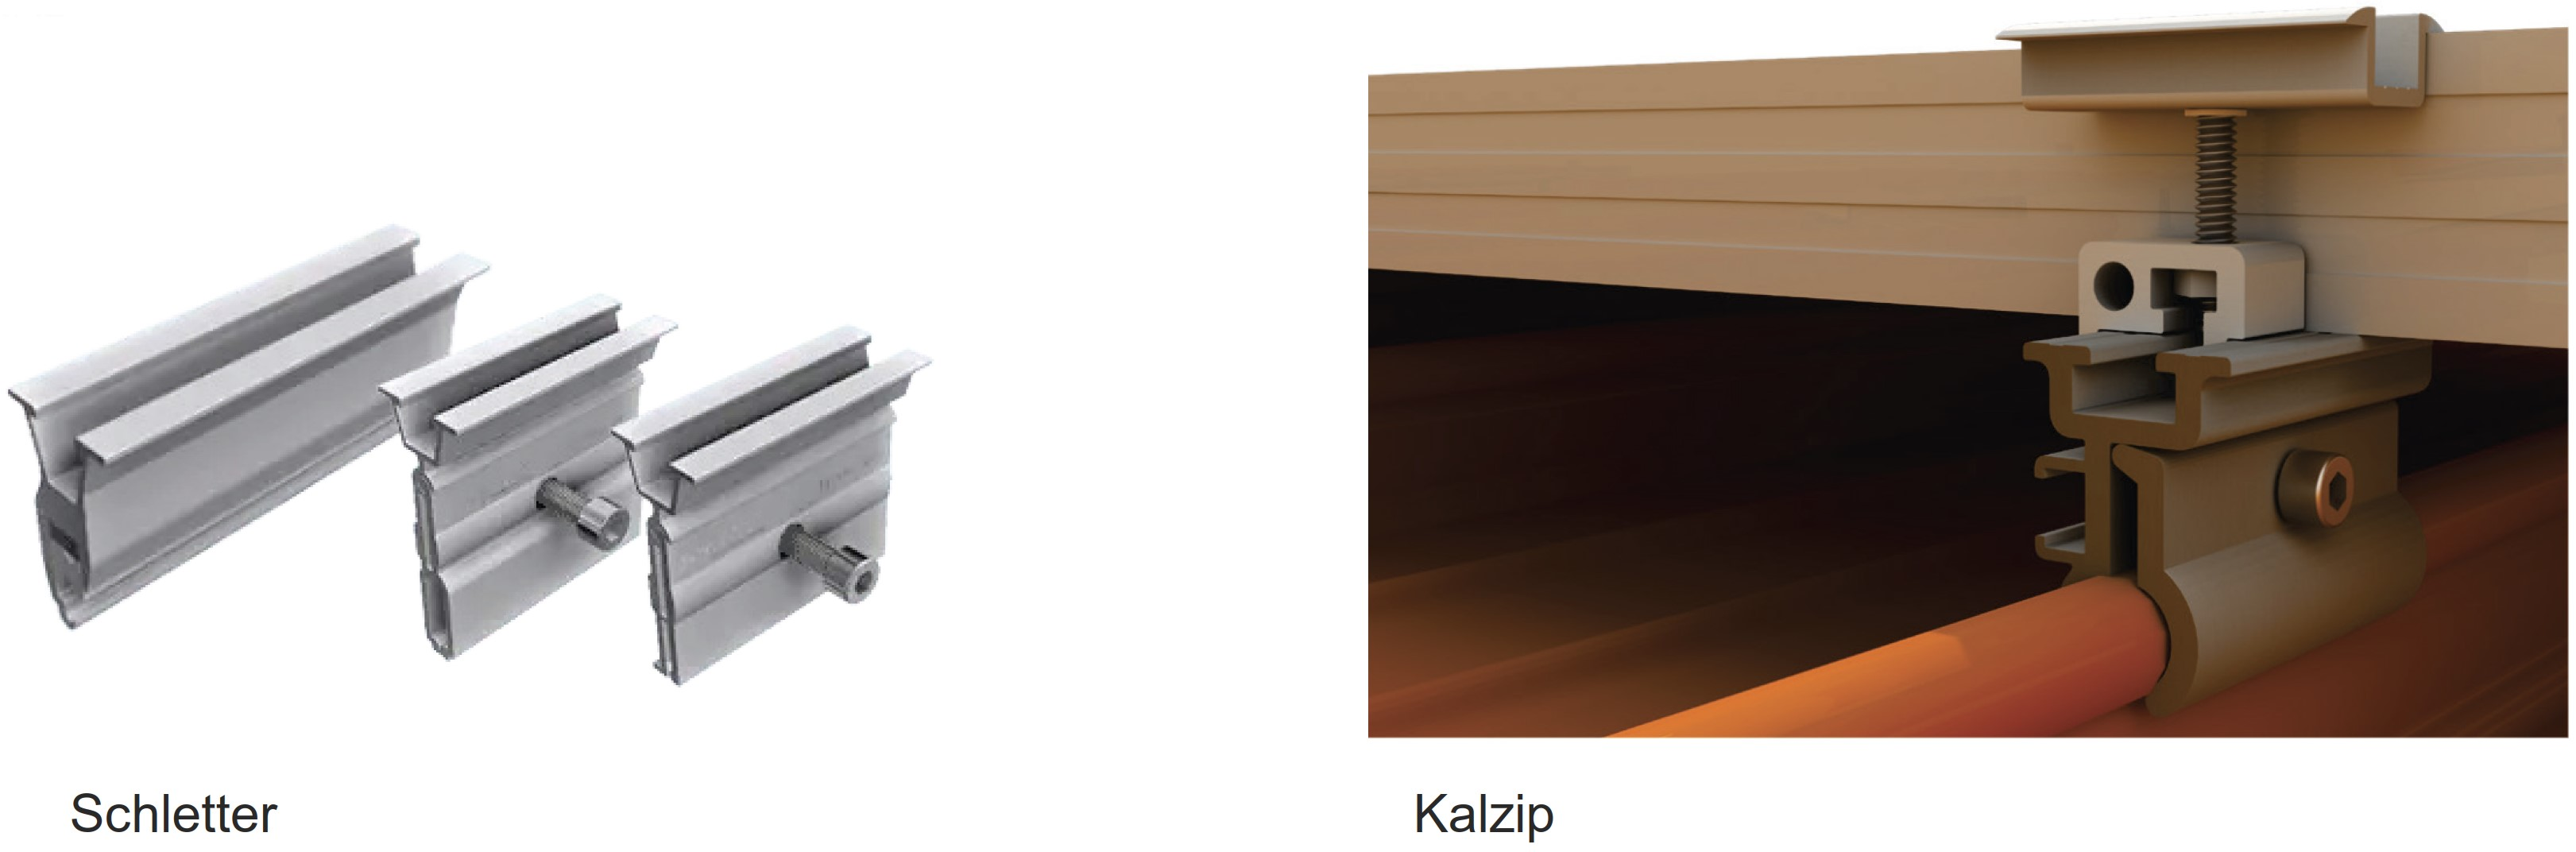
\includegraphics[width=0.95\columnwidth]{images/Stehfalzklemmen.jpg}


\subsubsection{Nieten, Blechschrauben}
Für Trapezblechdächer\\
\begin{minipage}[t]{0.48\columnwidth}
    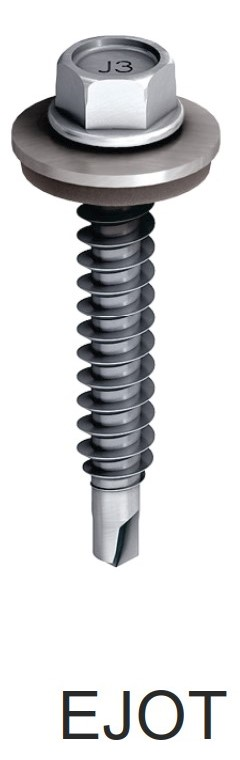
\includegraphics[width=0.15\columnwidth]{images/Nieten_Blechschrauben_1.jpg}
\end{minipage}
\hfill
\begin{minipage}[t]{0.48\columnwidth}
    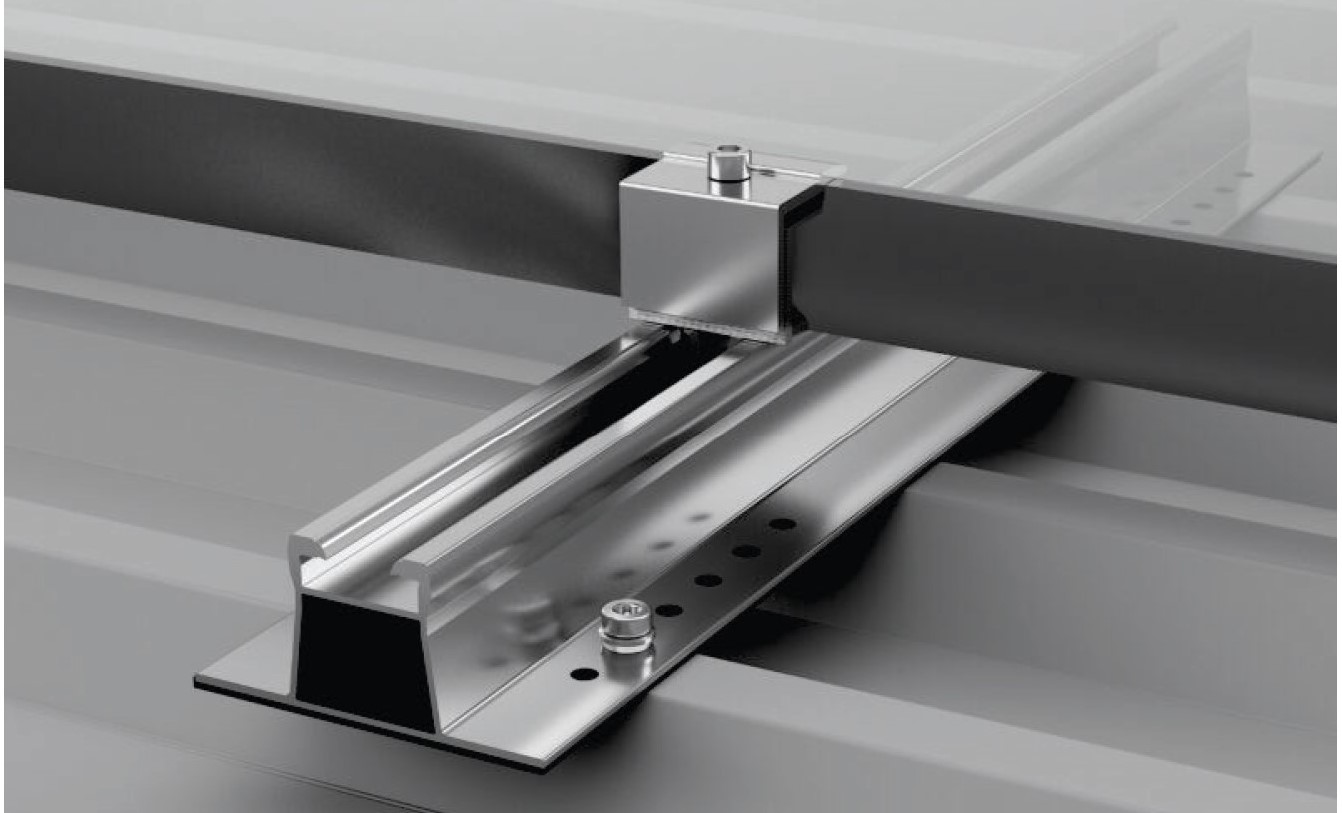
\includegraphics[width=0.85\columnwidth]{images/Nieten_Blechschrauben_2.jpg}
\end{minipage}



\subsection{Tragkonstruktion / Schienensystem}

\subsubsection{Einlagiges Schienensystem}

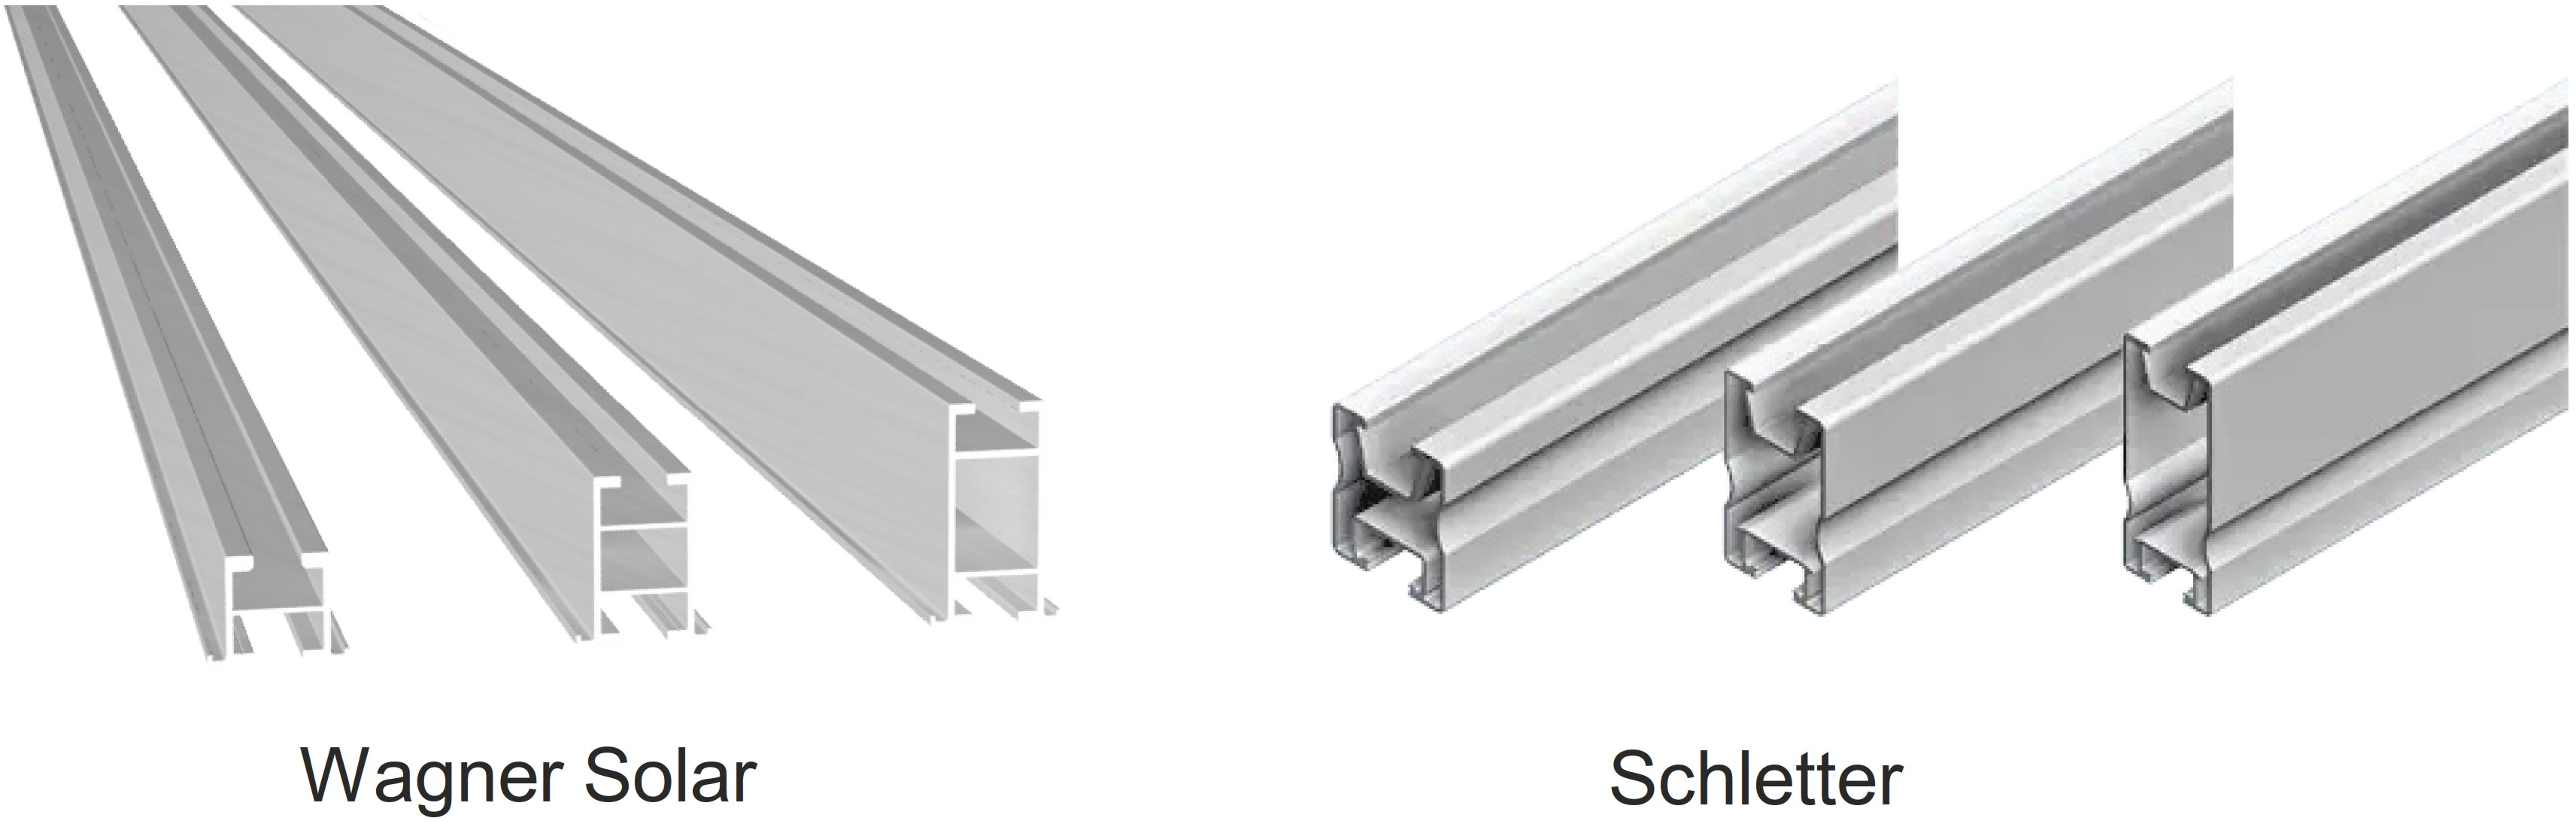
\includegraphics[width=0.85\columnwidth]{images/Einlagiges Schienensystem 1.jpg}\\

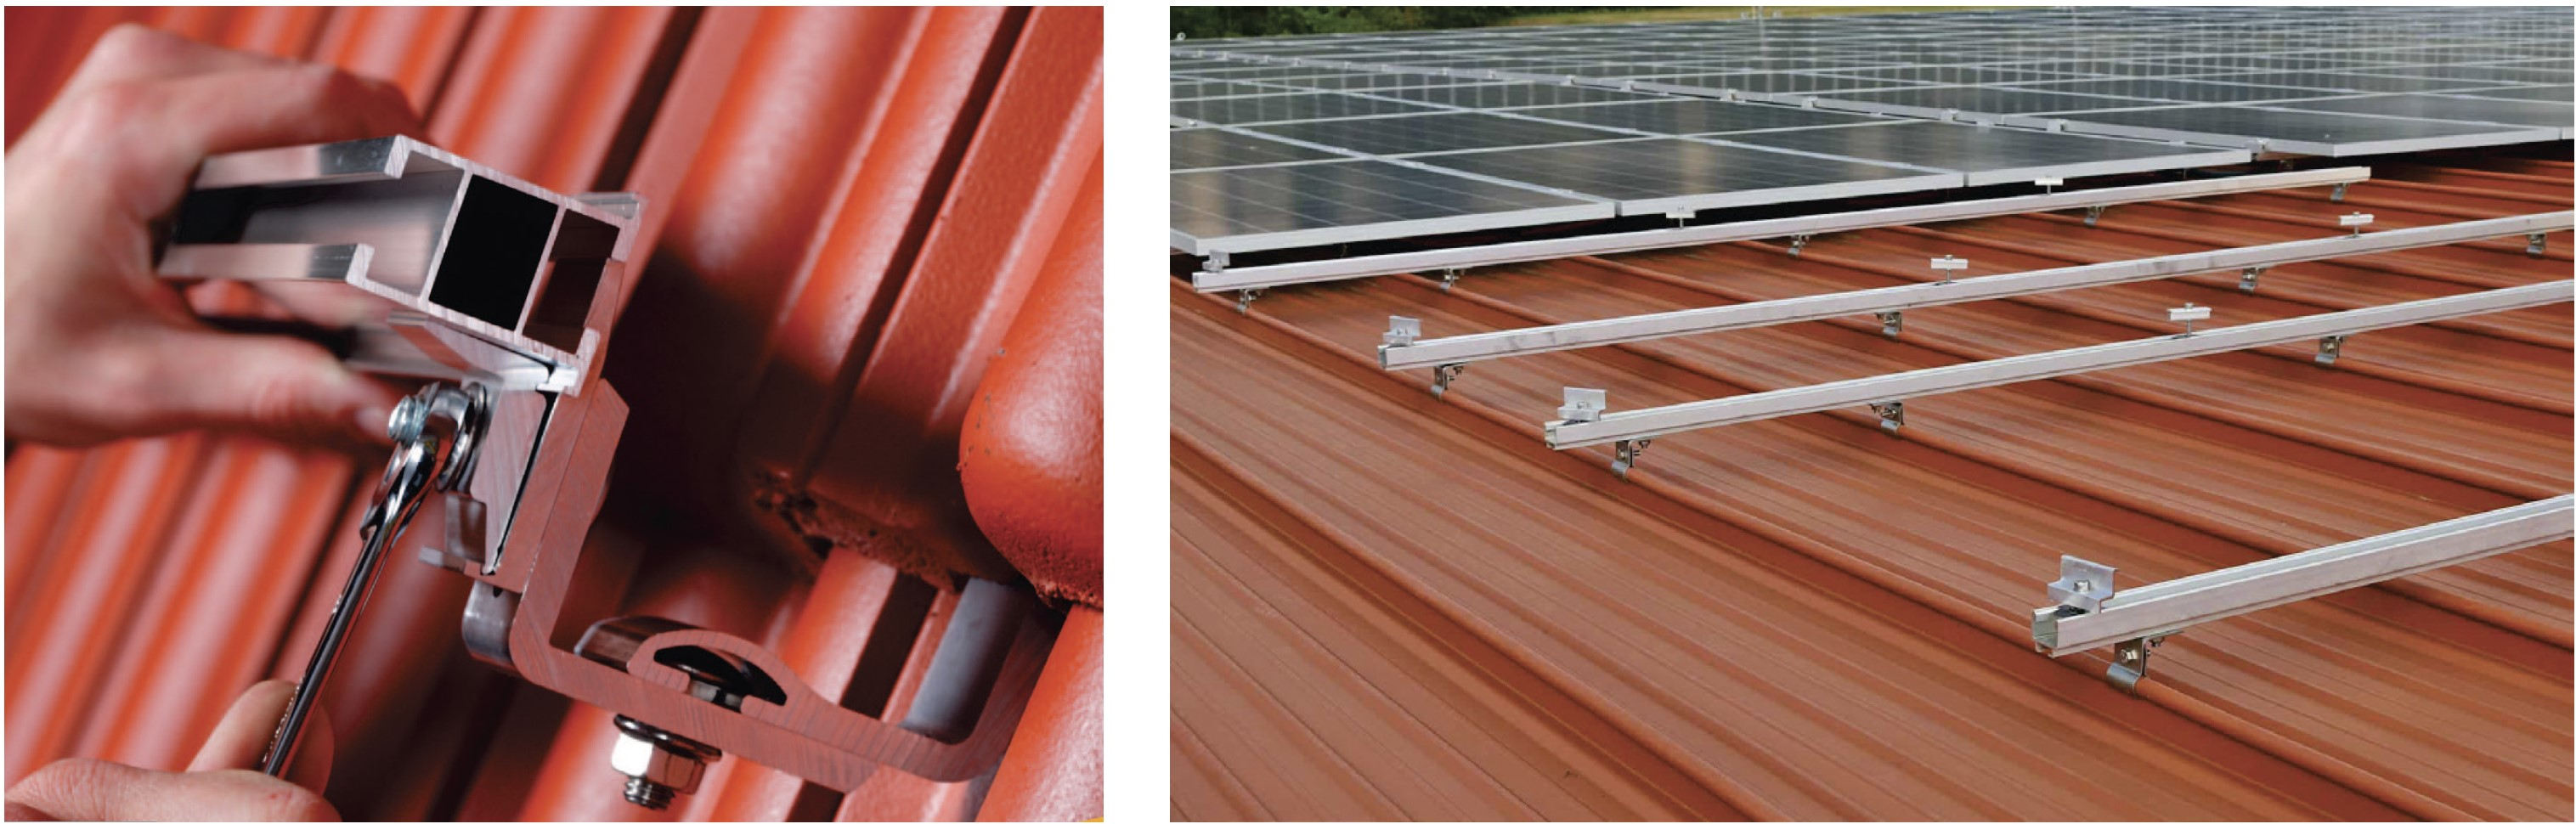
\includegraphics[width=0.85\columnwidth]{images/Einlagiges Schienensystem 2.jpg}


\subsubsection{Zweilagiges Schienensystem (Kreuzverbund)}
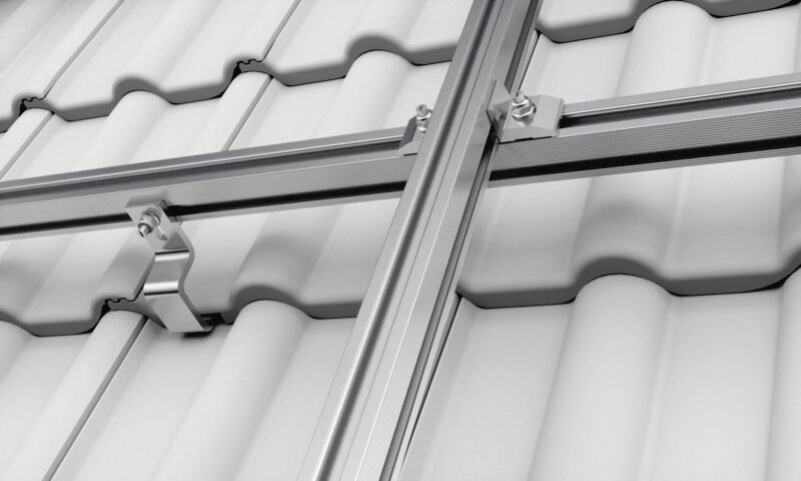
\includegraphics[width=0.48\columnwidth]{images/Zweilagiges Schienensystem (Kreuzverbund).png}



\subsection{Modulbefestigung}
\subsubsection{Modulklemmen}
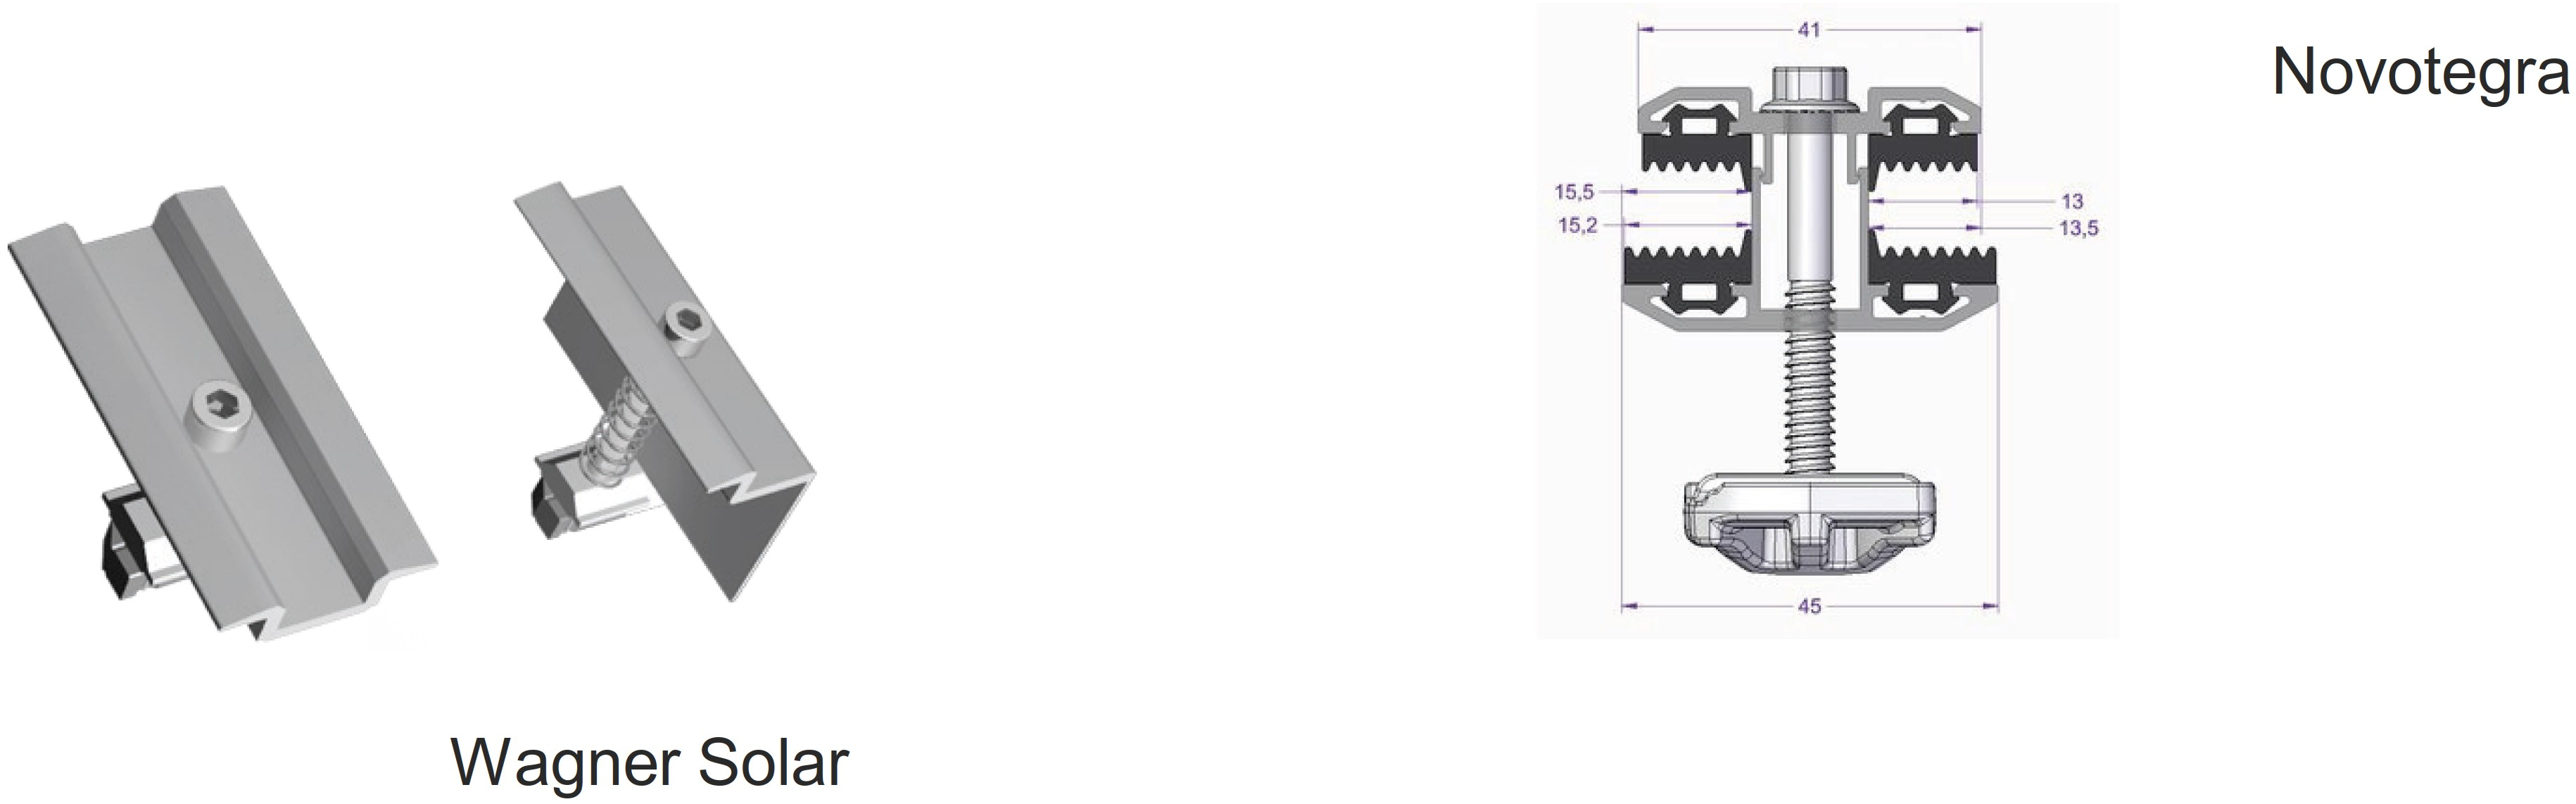
\includegraphics[width=0.95\columnwidth]{images/Modulklemmen.jpg}


\subsubsection{Einlegesystem}
\begin{minipage}[t]{0.48\columnwidth}
    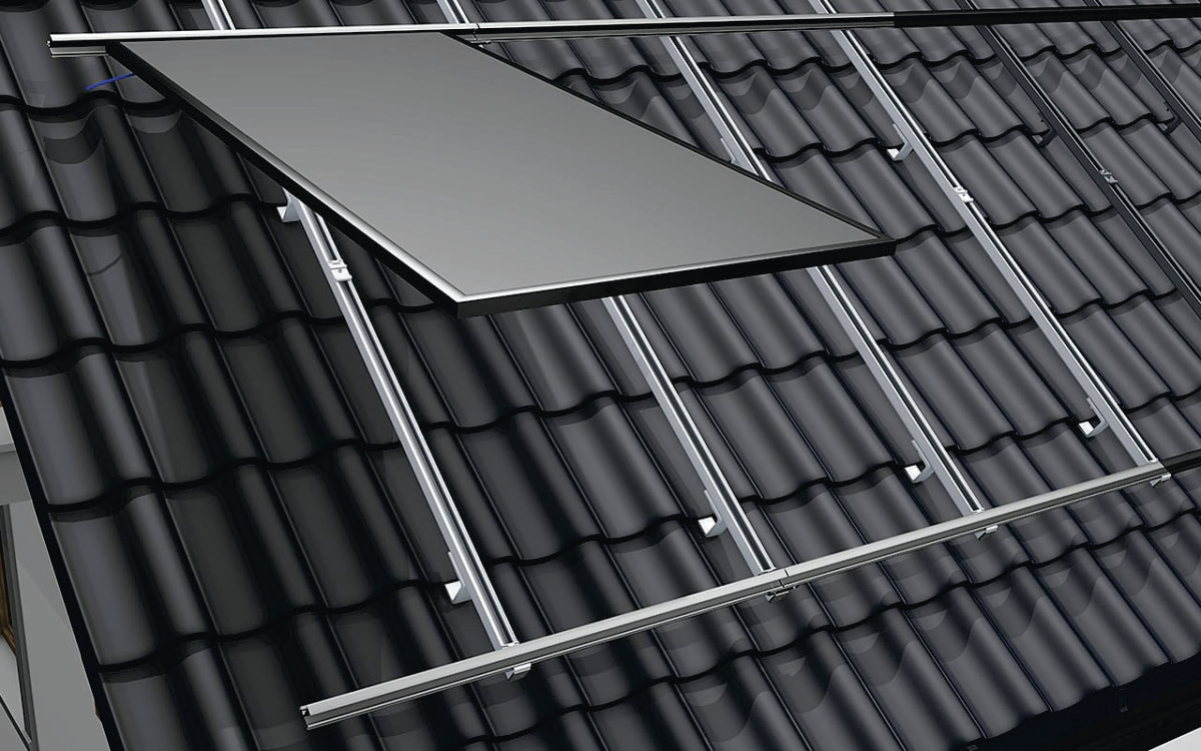
\includegraphics[width=0.95\columnwidth]{images/Einlegesystem_1.png}
\end{minipage}
\hfill
\begin{minipage}[t]{0.48\columnwidth}
    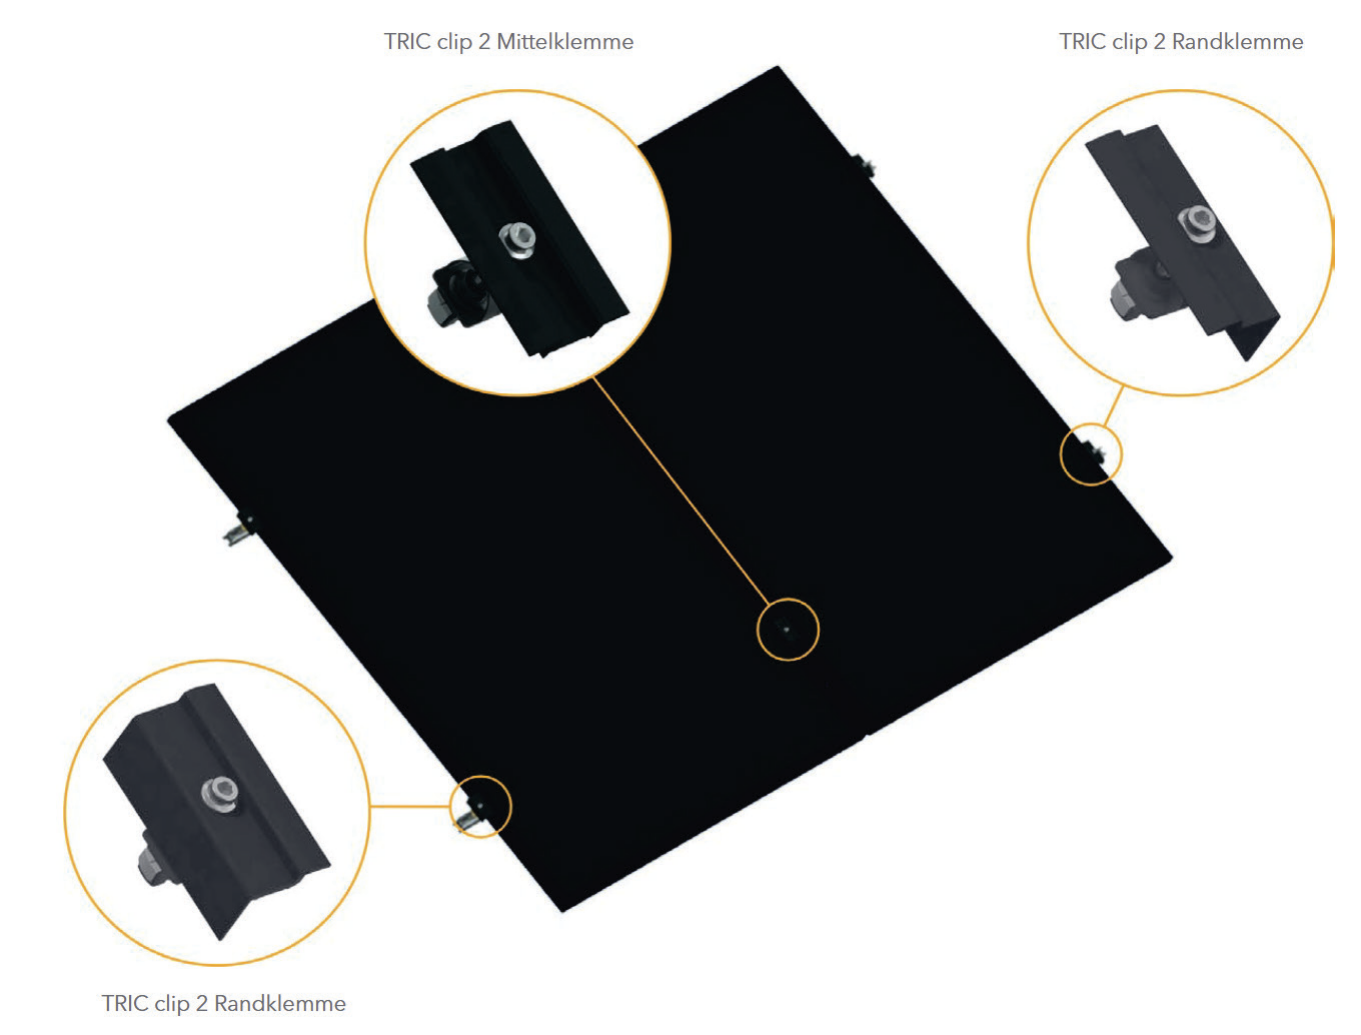
\includegraphics[width=0.95\columnwidth]{images/Einlegesystem_2.png}
\end{minipage}



\subsection{Zubehör}

\subsubsection{Kabelführung}
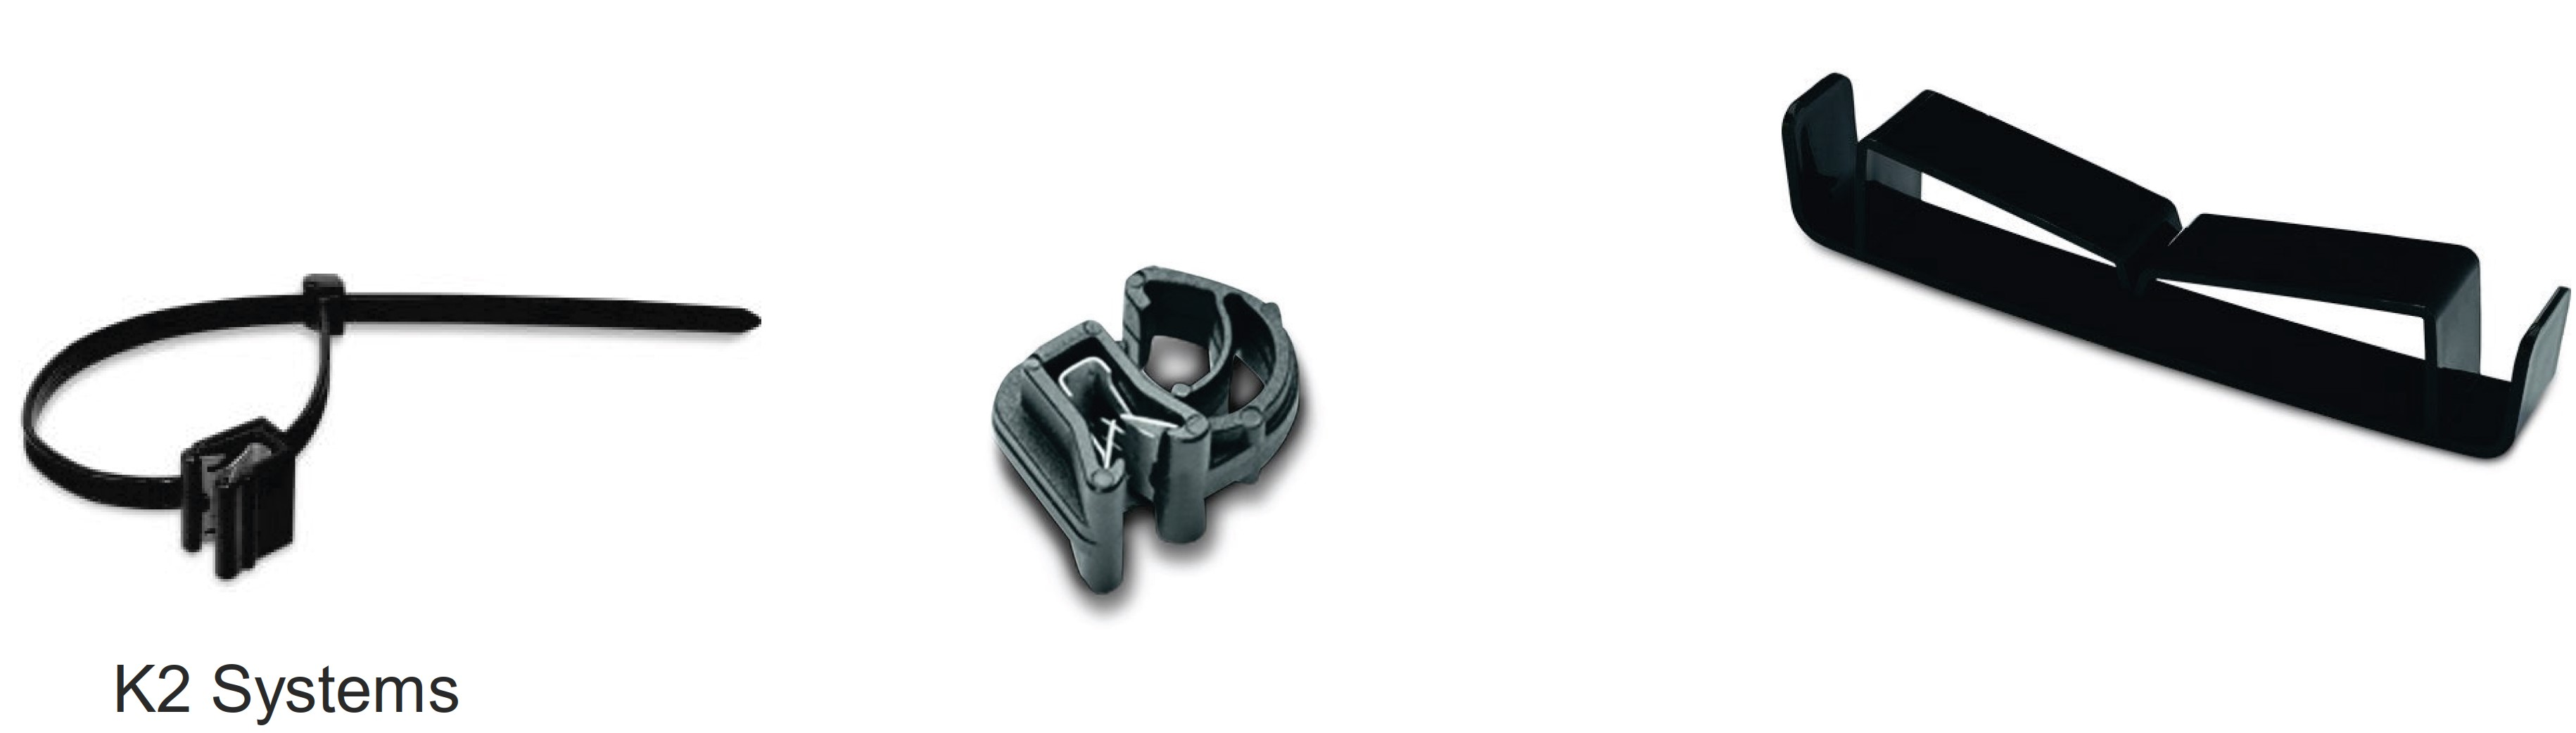
\includegraphics[width=0.95\columnwidth]{images/Kabelführung_1.jpg}\\
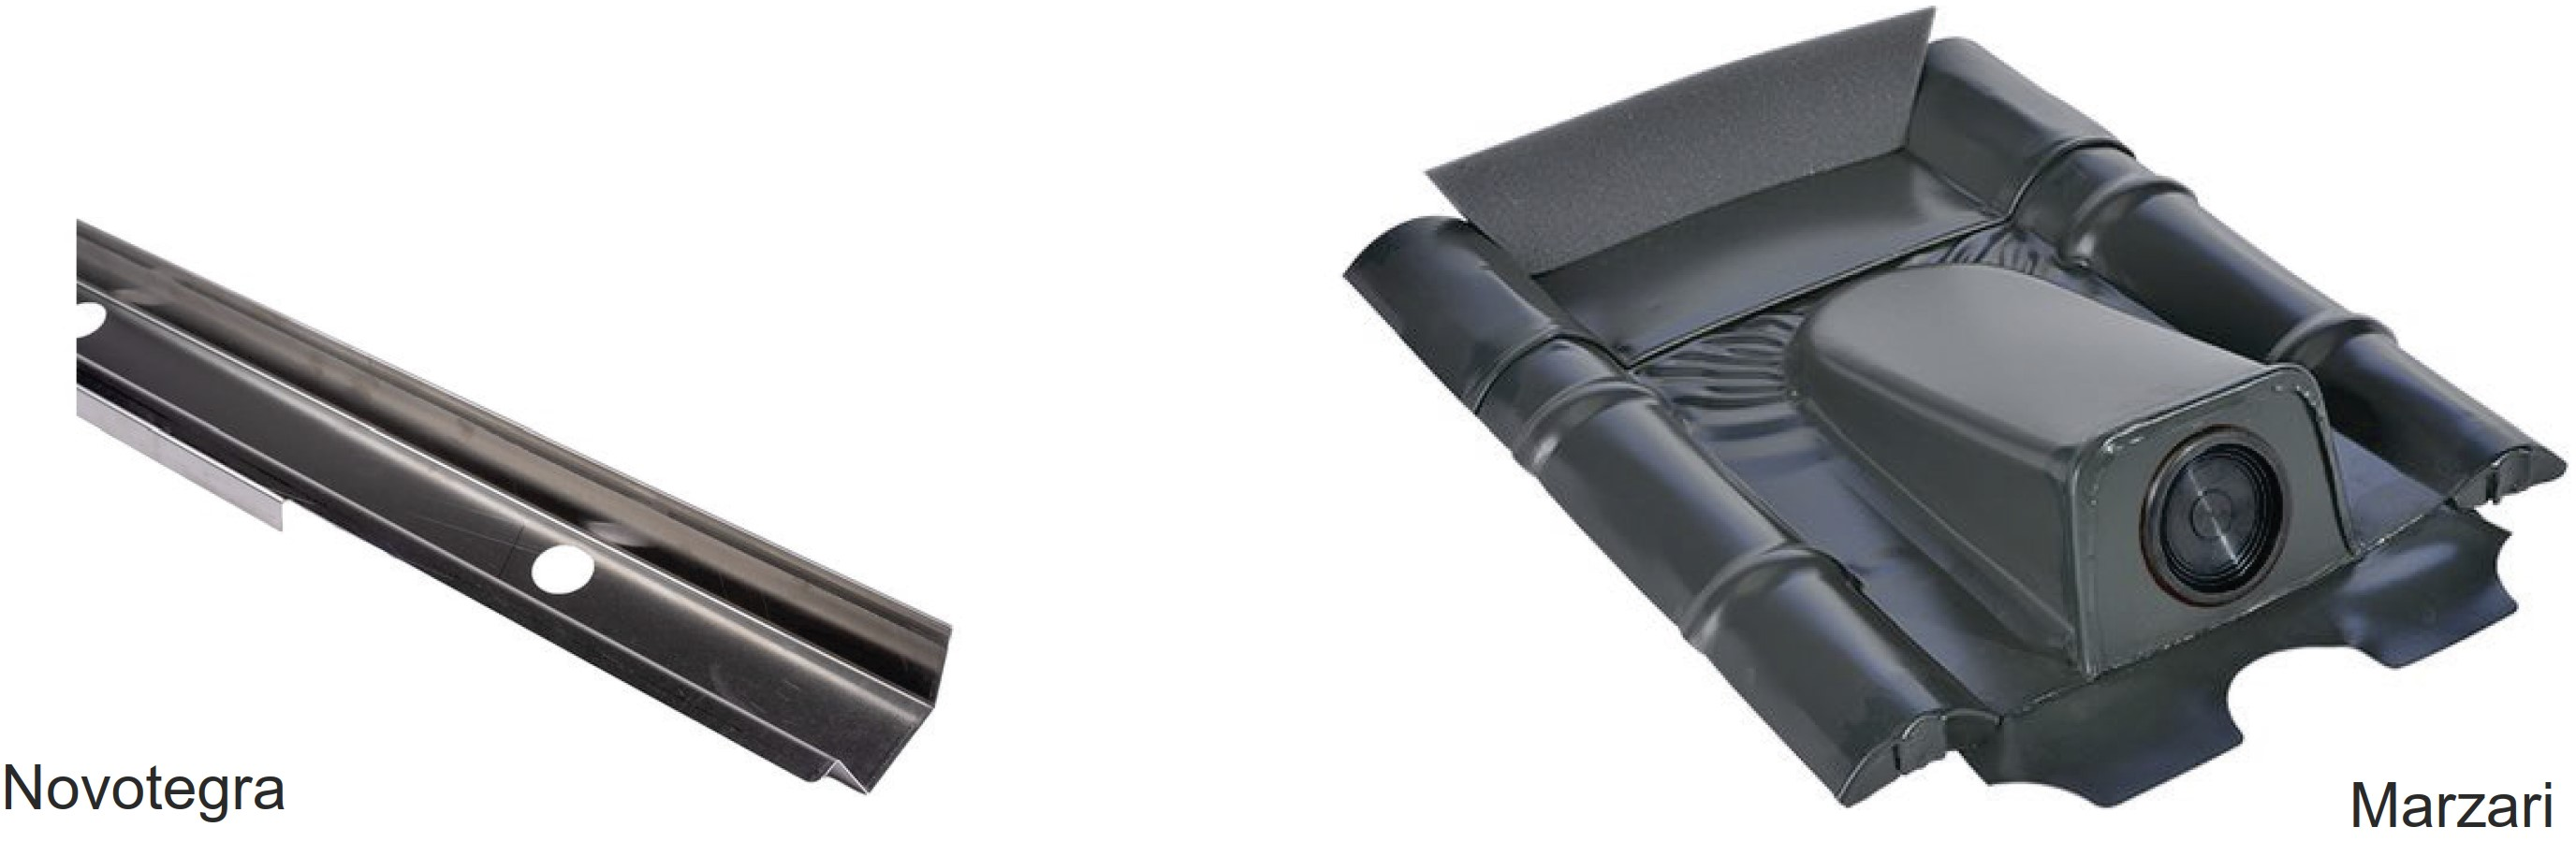
\includegraphics[width=0.95\columnwidth]{images/Kabelführung_2.jpg}


\subsubsection{Schneefang}
\begin{minipage}[t]{0.48\columnwidth}
    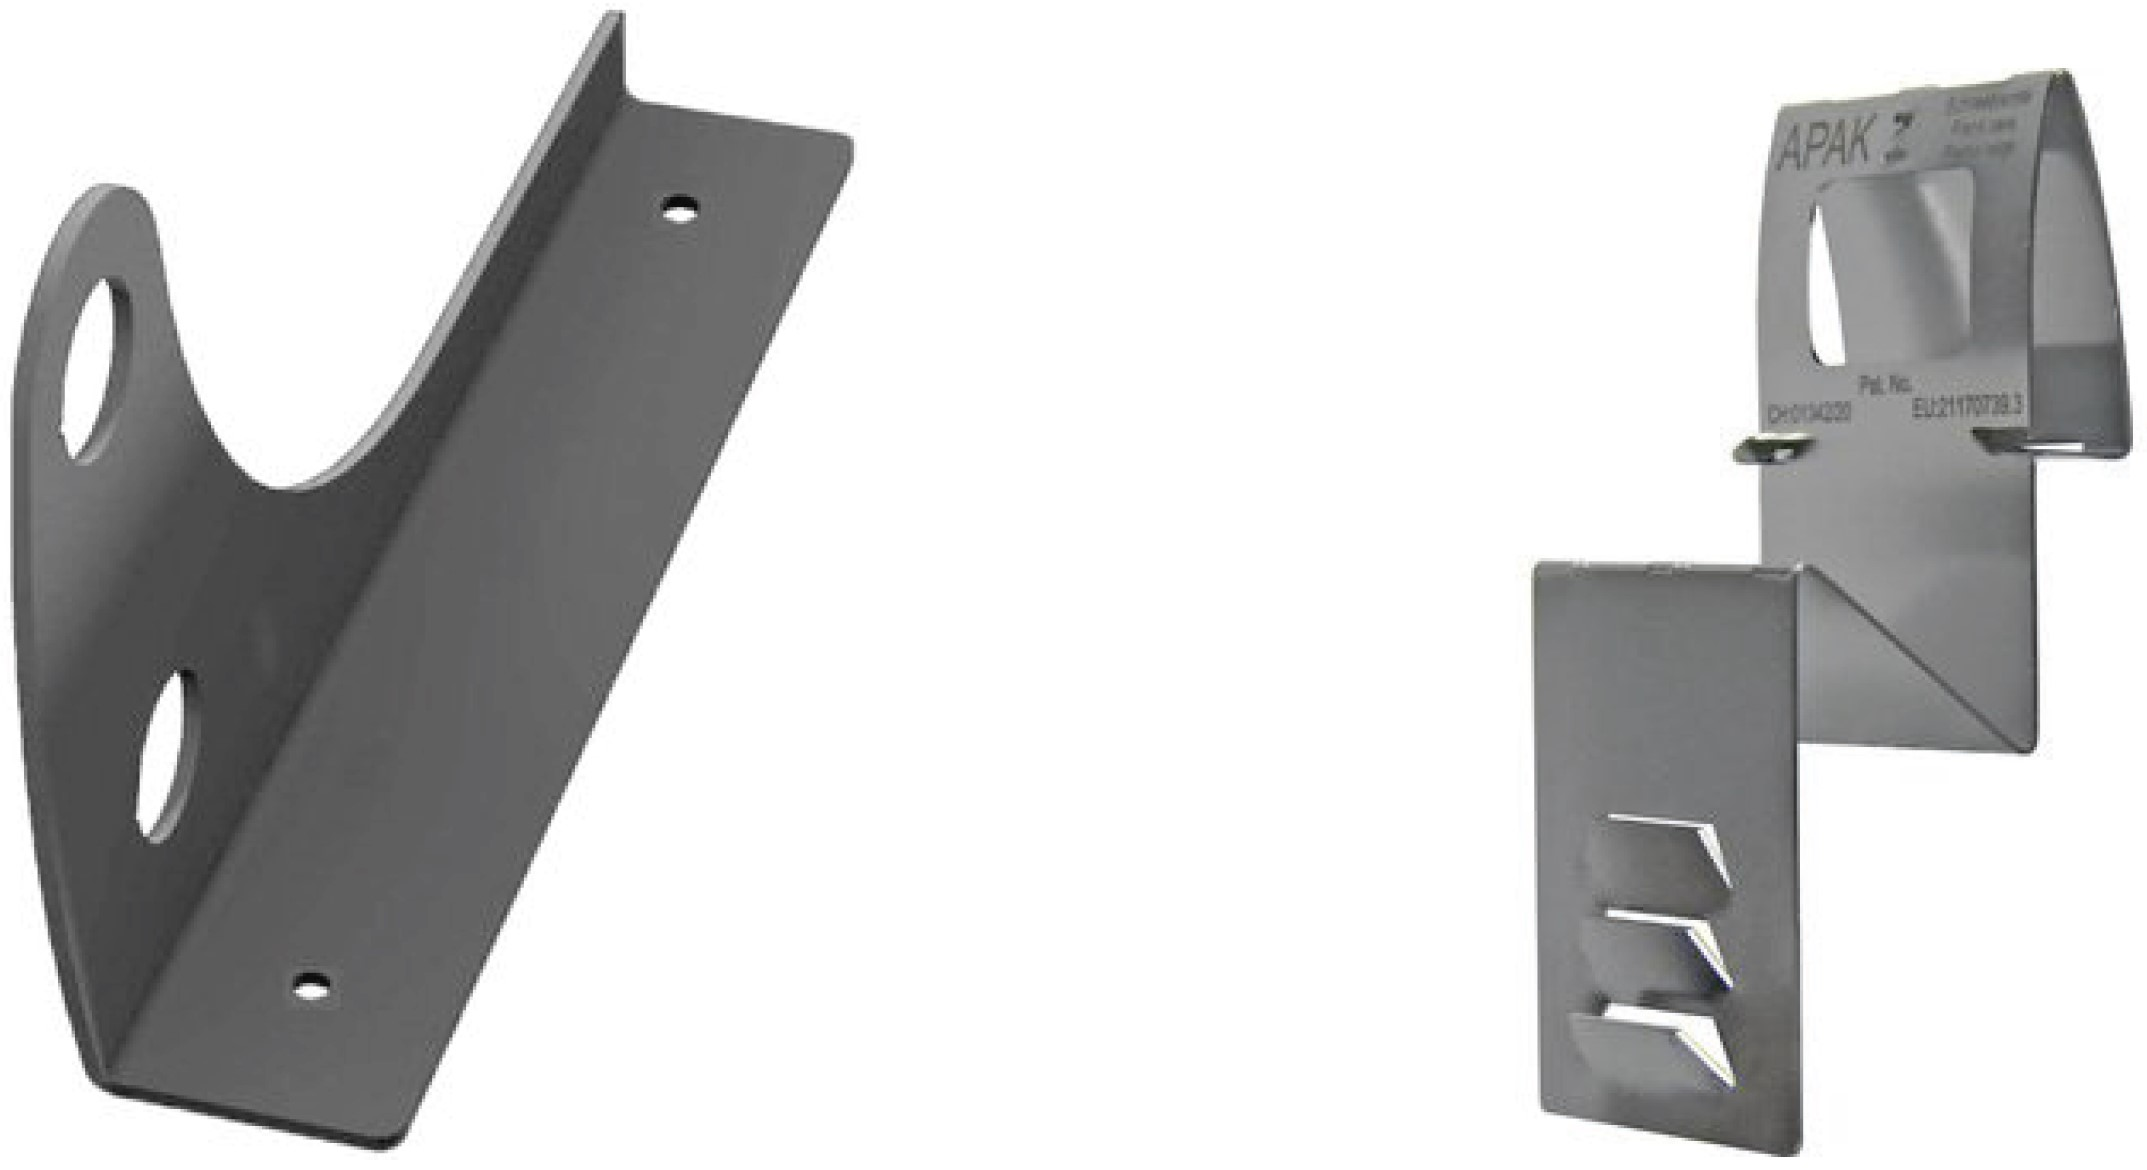
\includegraphics[width=0.95\columnwidth]{images/Schneefang_1.jpg}
\end{minipage}
\hfill
\begin{minipage}[t]{0.48\columnwidth}
    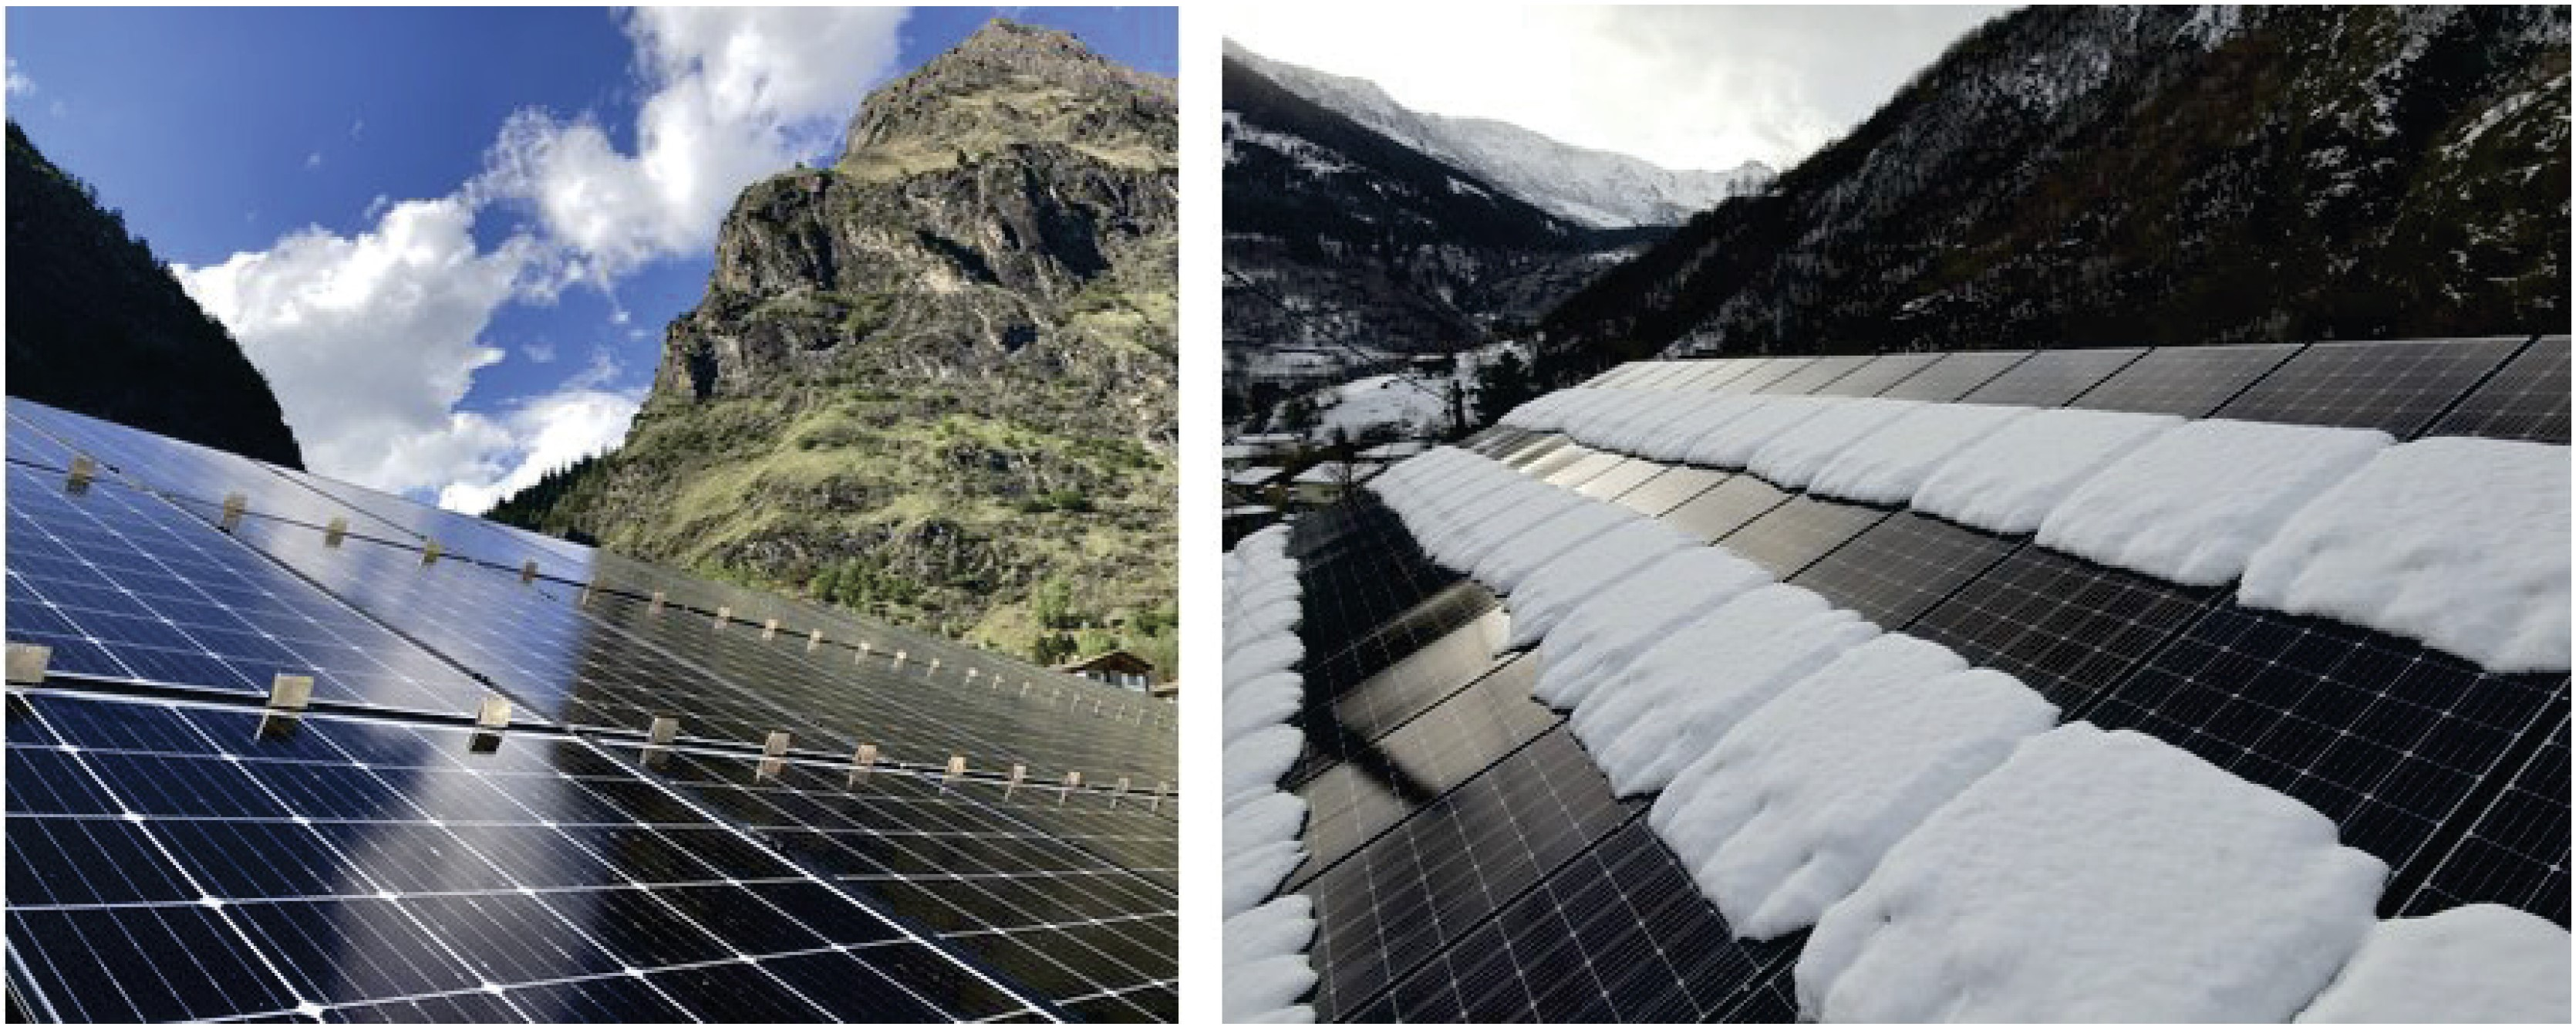
\includegraphics[width=0.95\columnwidth]{images/Schneefang_2.jpg}
\end{minipage}

%\end{comment}
\subsection{Blitzschutz und Erdung}

\begin{minipage}[c]{0.28\columnwidth}
    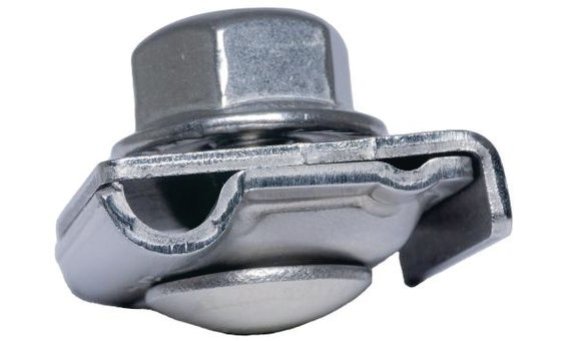
\includegraphics[width=0.95\columnwidth]{images/Blitzschutz.png}
\end{minipage}
\hfill
\begin{minipage}[c]{0.68\columnwidth}
    \textbf{Pflicht:}
        \begin{itemize}
            \item Blitzschutz vorhanden, Gebäudehöhe überragt
            \item Metallische Modulrahmen, nicht Schutzklasse II
            \item Überspannungsschutz fordert explizite Erdung
    \end{itemize}

    \textbf{Freiwillig:}
        \begin{itemize}
            \item Niedrige Gebäude, kein Blitzschutz vorhanden
            \item Module Schutzklasse II, isolierte Montage
        \end{itemize}

    \textbf{Immer beachten:}
        \begin{itemize}
            \item Lokale Netzbetreibervorgaben
        \end{itemize}
\end{minipage}



\subsection{Statik}
\subsubsection{Nachweise}
\begin{outline}
    \1 Dass das Dach die zusätzlichen Auflasten aufnehmen kann
    \1 PV-Module und Montagesystem
        \2 Grundlage: SIA 261 \glqq Einwirkungen auf Tragwerke\grqq
            \3 Berechnung der einwirkenden Wind- und Schneelasten
        \2 Windlasten
            \3 Entscheidend meistens Windsogkräfte
            \3 Unterscheidung in Dachmittel-, Rand- und Eckbereich
            \3 U.a. abhängig von Gebäudehöhe und Bodenrauigkeit
        \2 Zu berücksichtigende Schneelast insbesondere abhängig von
            \3 Dachneigung und Dachform
            \3 Höhenlage und Bezugshöhe
\end{outline}
\begin{comment}
    
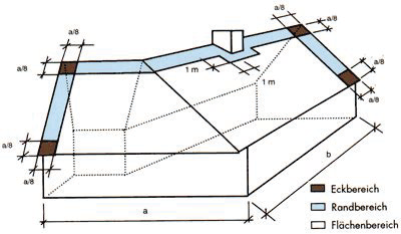
\includegraphics[width=0.75\columnwidth]{images/Statik.png}


\subsubsection{Beispiel Schneelasten}
\textbf{SIA 261 Anhang D “Bezugshöhe für Schneelasten”}\\
Bezugshöhe \(h_0\), (nicht anwendbar auf Bauwerke über 2000 m Meereshöhe)

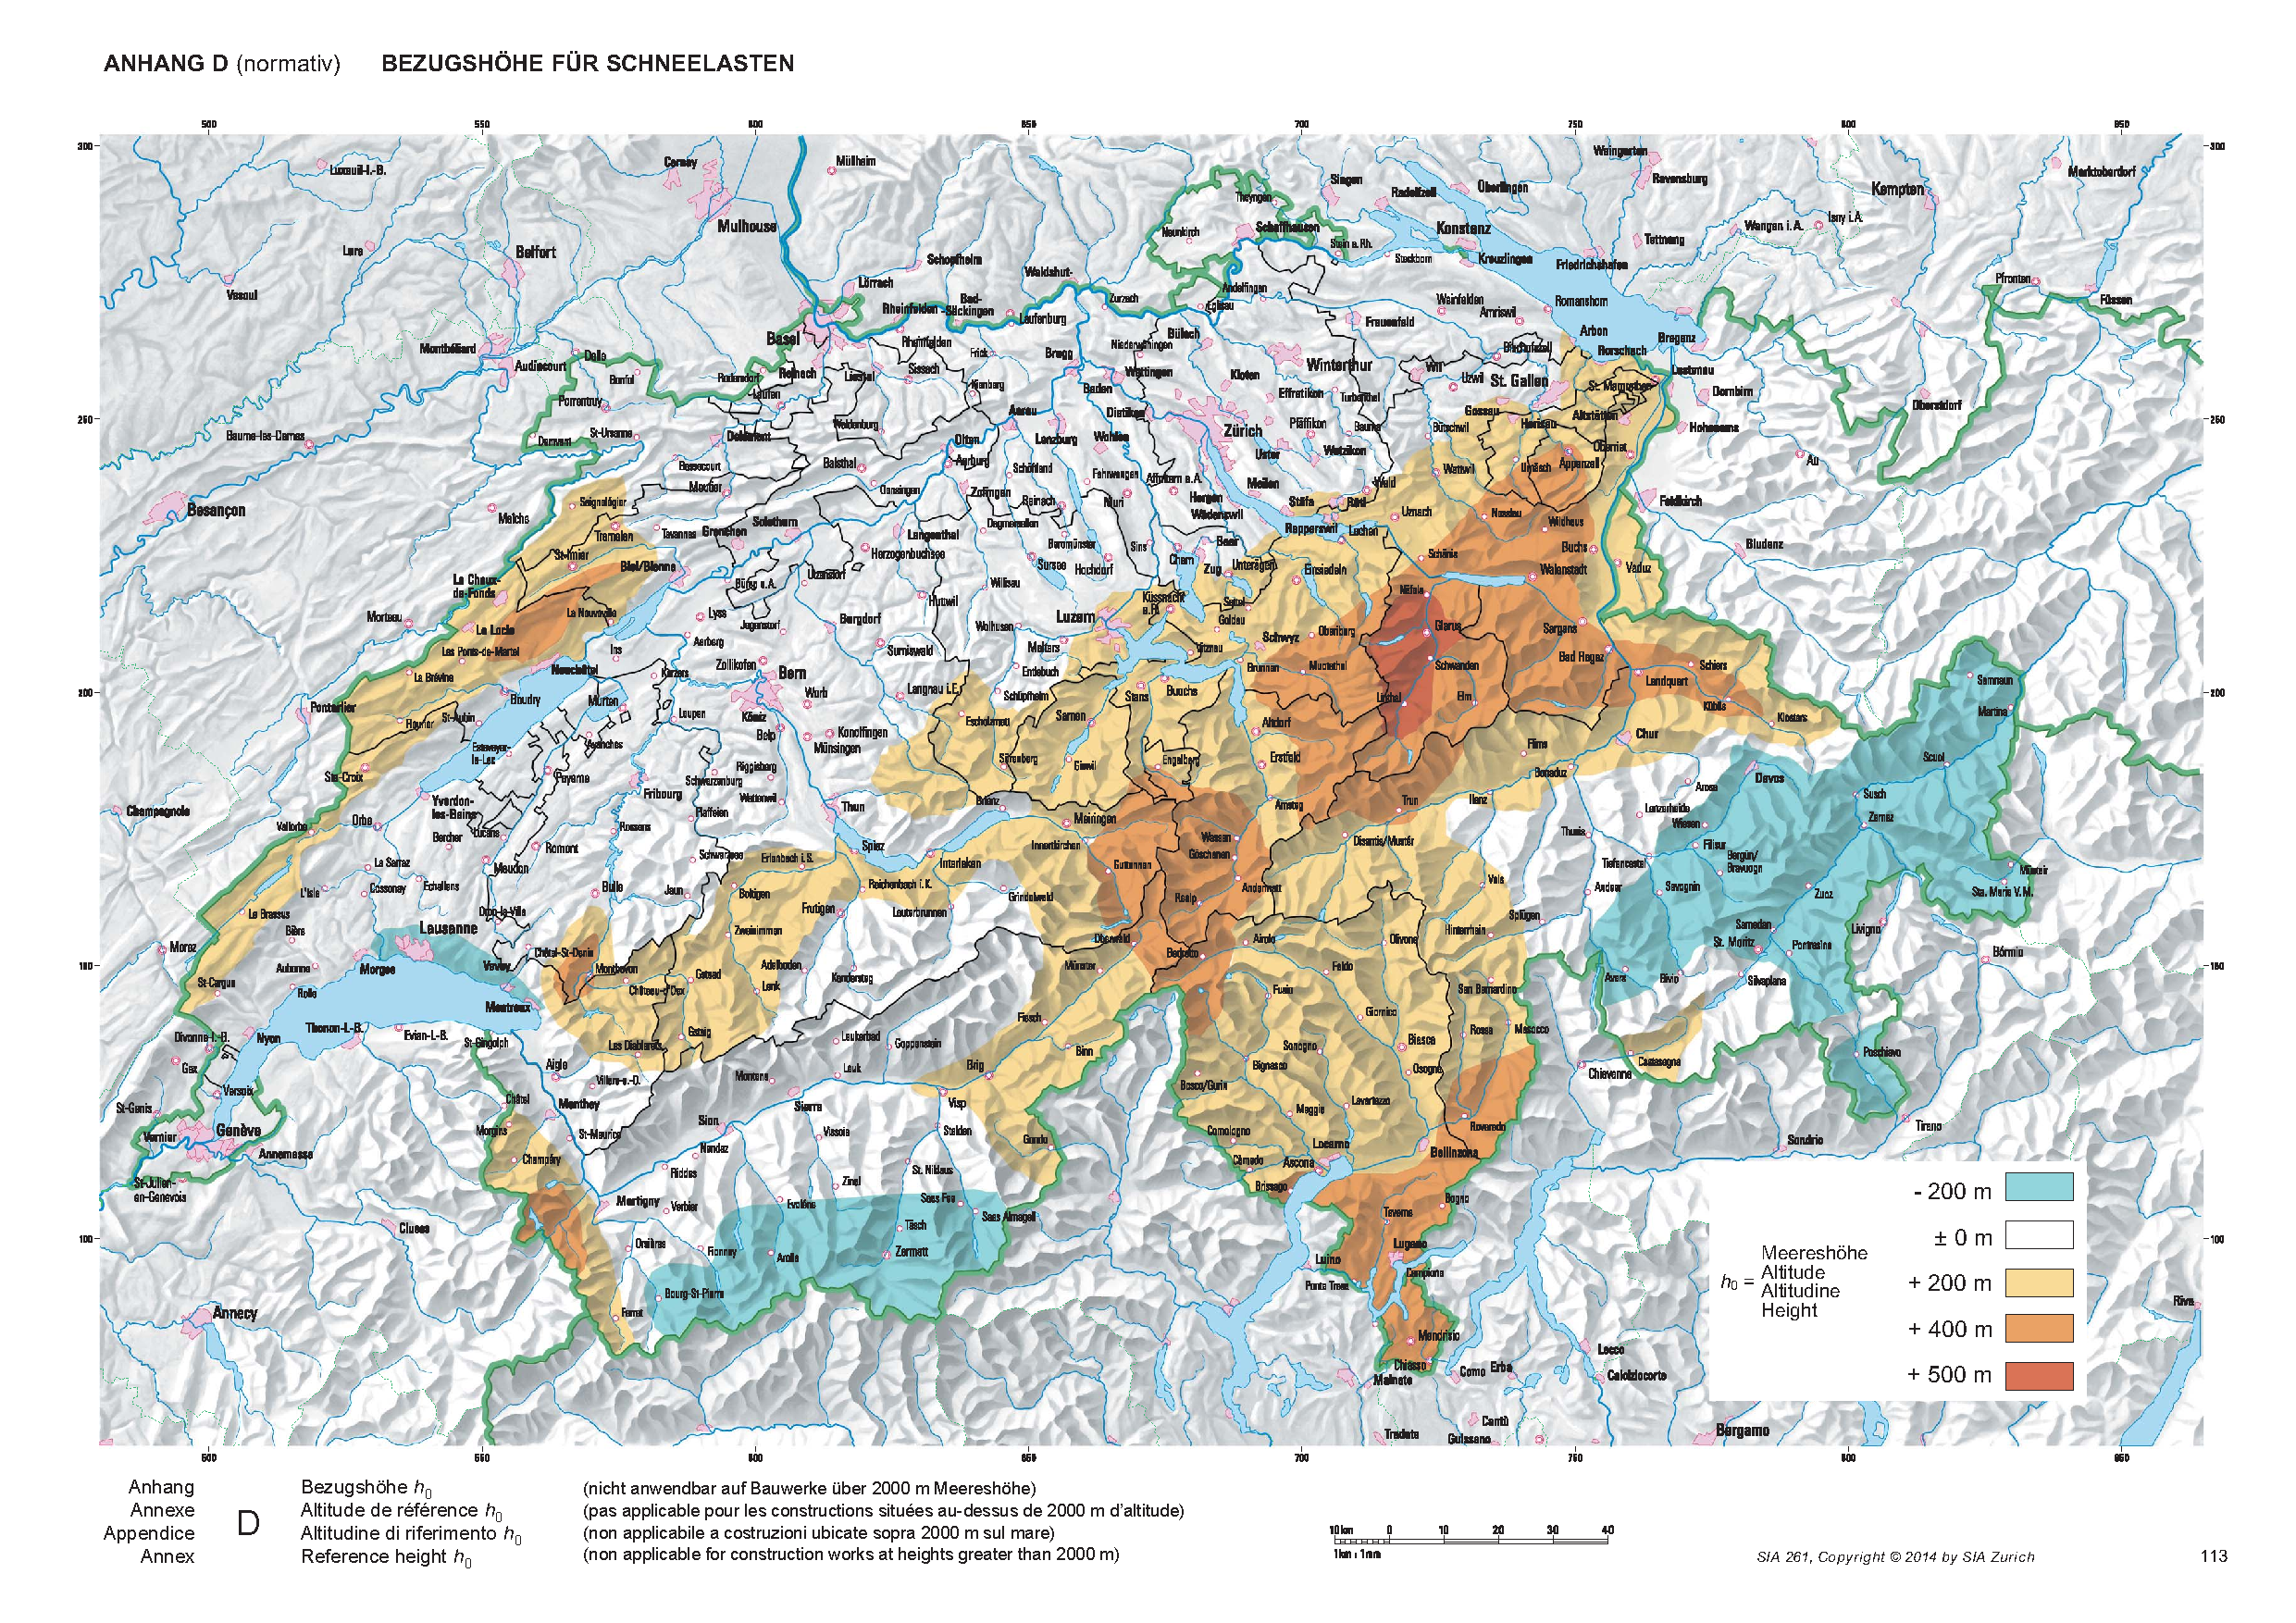
\includegraphics[width=1\columnwidth]{images/261_2014_d_Anhang_D.PDF}

\end{comment}
        \columnbreak
\section{Anlagetypen}

\subsection{Klassifizierung}

\begin{outline}
    \1 Aufdachanlagen
        \2 Schrägdach
    \1 Indachanlagen
    \1 Flachdachanlagen
        \2 Typischerweise Befestigung durch Beschwerung (keine Dachdurchdringung)
            \3 Aerodynamische Systeme
            \3 Flacher Aufbau
            \3 Verbindung der Reihen
        \2 Meist Ost-West-Ausrichtung, ca. 10--15° Neigung
        \2 Aplin
            \3 Vertikal Bifazial
            \3 Solartanne
    \1 Fassadenanlagen
        \2 Herausforderungen:
            \3 Statik (geprüftes Gesamtsystem oder Prüfung im Einzelfall)
            \3 Brandschutz (Brände breiten sich vertikal schneller aus)
            \3 Optik (Farbe, Form, Haptik, Reflexion/Blendung)
            \3 Wartung und Zugänglichkeit Technik
    \1 Freiflächenanlagen
    \1 Weitere / neue Konzepte
        \2 Infrastruktur 
            \3 Parkplatzüberdachung
            \3 Lärmschutzwände
            \3 Staudämme
            \3 Solarfaltdach auf ARA 
        \2 Agri-PV
            \3 Müssen nach Raumplanungsverordnung (RPV) Art. 32c in wenig empfindlichen Gebieten Vorteile für die landwirtschaftliche Produktion bewirken oder entsprechenden Versuchs- und Forschungszwecken dienen.
        \2 Floating-PV
        \2 Fahrzeugintegrierte PV (Vehicle Integrated PV -- VIPV)
        \2 Plug\&Play PV (Stecker-PV)
            \3 Bis 600 W AC-Ausgangsleistung des Wechselrichters
  \end{outline}


\subsection{Bifaziale Module}
Beide Seiten des Moduls zur Stromerzeugung genutzt!\\

\vspace{0.25cm}

\subsubsection{Prinzipschema}
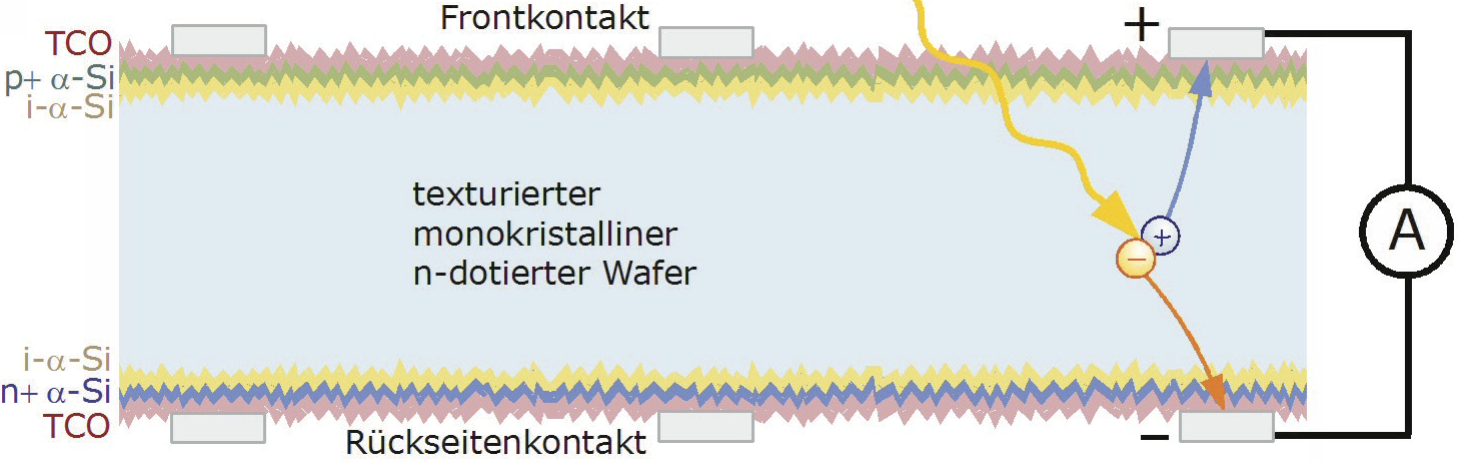
\includegraphics[width=0.95\columnwidth]{images/Bifaziale Module 1.png}

\vspace{0.25cm}

\subsubsection{Funktionsprinzip}
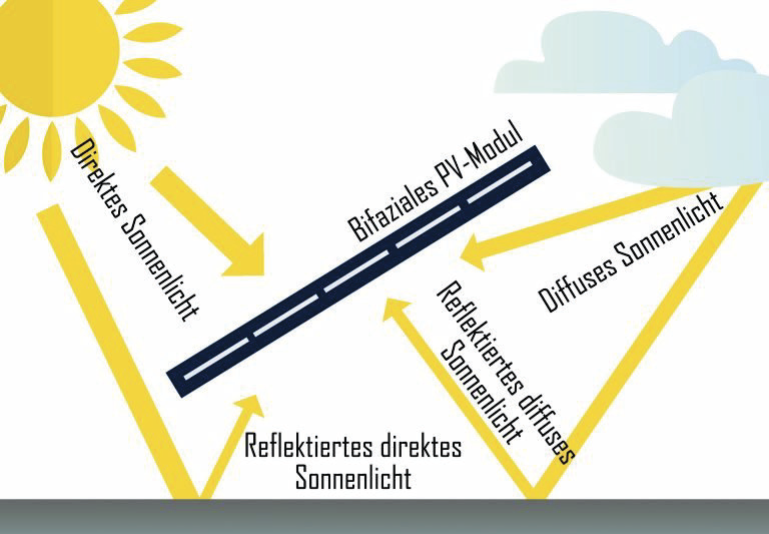
\includegraphics[width=0.5\columnwidth]{images/Bifaziale Module 2.png}


























        \section{PV Stromerzeugung und Verbrauch}































        \columnbreak
\section{Batteriespeicher}
\subsection{Kennzahlen bei PV-Eigenverbrauchssteigerung}

\subsubsection{Energieverbrauch}

\vspace{0.1cm}

$
\boxed{
E_\mathrm{ges} = E_{\mathrm{PV,AC}} - E_{\mathrm{NE}} + E_{\mathrm{NB}} 
}
$
$
\boxed{
E_\mathrm{eig} = E_{\mathrm{PV,AC}} - E_{\mathrm{NE}}
}
$

\vspace{0.1cm}

$
\boxed{
R_\mathrm{eig} = \frac{E_\mathrm{eig}}{E_\mathrm{PV,AC}}
}
$
$
\boxed{
R_\mathrm{eig} = \frac{E_\mathrm{PV,AC} - E_\mathrm{NE}}{E_\mathrm{PV,AC}}
}
$
$
\boxed{
R_\mathrm{eig} = \frac{E_\mathrm{ges} - E_\mathrm{NB}}{E_\mathrm{PV,AC}}
}
$

\vspace{0.1cm}

$
\boxed{
R_\mathrm{aut,ges} = \frac{E_\mathrm{eig}}{E_\mathrm{ges}} 
}
$
$
\boxed{
R_\mathrm{aut,ges} = \frac{E_\mathrm{ges} - E_\mathrm{NB}}{E_\mathrm{ges}}
}
$

\vspace{0.1cm}

$
\boxed{
R_\mathrm{aut,Last} = \frac{E_\mathrm{eig,PV} + E_\mathrm{eig,BE}}{E_\mathrm{Last}}
}
$
$
\boxed{
R_\mathrm{aut,Last} = \frac{E_\mathrm{Last} - E_\mathrm{NB}}{E_\mathrm{Last}}
}
$

\vspace{0.1cm}

$
\boxed{
R_\mathrm{PV} = \frac{E_\mathrm{PV,AC}}{E_\mathrm{ges}}
}
$

\vspace{0.1cm}

\renewcommand{\arraystretch}{1.2}
\begin{tabular}{@{} l p{6.5cm} l @{}}
    $[E_\mathrm{PV,AC}]$   & PV-Ertrag (AC, gesamt) \dotfill & $\mathrm{kWh}$ \\
    $[E_\mathrm{eig}]$     & Eigenverbrauch (Direktverbrauch und Batterieladung) \dotfill & $\mathrm{kWh}$ \\
    $[E_\mathrm{eig,PV}]$  & PV-Direktverbrauch \dotfill & $\mathrm{kWh}$ \\
    $[E_\mathrm{eig,BE}]$  & Batterieentladung \dotfill & $\mathrm{kWh}$ \\
    $[E_\mathrm{ges}]$     & Elektrischer Gesamtenergieverbrauch \dotfill & $\mathrm{kWh}$ \\
    $[E_\mathrm{Last}]$    & Elektrische Last \dotfill & $\mathrm{kWh}$ \\
    $[E_\mathrm{NE}]$      & Netzeinspeisung \dotfill & $\mathrm{kWh}$ \\
    $[E_\mathrm{NB}]$      & Netzbezug \dotfill & $\mathrm{kWh}$ \\
    $[R_\mathrm{eig}]$     & Eigenverbrauchsquote \dotfill & $-$ \\
    $[R_\mathrm{aut}]$     & Autarkiegrad \dotfill & $-$ \\
    $[R_\mathrm{PV}]$      & PV-Ertragsverhältnis \dotfill & $-$ \\
\end{tabular}

\vspace{0.1cm}

\textbf{Netto-Nullenergie Gebäude:} $R_\mathrm{PV} = 1$ und $R_\mathrm{eig} = R_\mathrm{aut,ges}$


\subsection{Zykleneffizienzen und Gesamtsystemeffizienz}

\subsubsection{DC-Zykleneffizienz}

\vspace{0.1cm}

$
\boxed{
\eta_\mathrm{Zykl,DC} = \frac{\mathrm{DC\text{-}Batterieentladung}}{\mathrm{DC\text{-}Batterieladung}}
}
$

\subsubsection{AC-Zykleneffizienz}

\vspace{0.1cm}

$
\boxed{
\eta_\mathrm{Zykl,AC} = \frac{\mathrm{AC\text{-}Batterieentladung}}{\mathrm{AC\text{-}Batterieladung}}
}
$

\subsubsection{Gesamtsystemeffizienz}

\vspace{0.1cm}

$
\boxed{
\eta_\mathrm{System} = \frac{\mathrm{AC\text{-}Gesamtenergiebereitstellung\text{-}Energieaufnahme\ PV\text{-}System}}{\mathrm{PV\ MPP\text{-}Angebot}}
}
$

\vspace{0.1cm}

\renewcommand{\arraystretch}{1.2}
\begin{tabular}{@{} l p{6.5cm} l @{}}
    $[\eta_\mathrm{Zykl,DC}]$   & DC-Zykleneffizienz \dotfill & $-$ \\
    $[\eta_\mathrm{Zykl,AC}]$   & AC-Zykleneffizienz \dotfill & $-$ \\
    $[\eta_\mathrm{System}]$    & Gesamtsystemeffizienz \dotfill & $-$ \\
\end{tabular}



\subsection{Bewertung von Batteriesystemen}

\subsubsection{System Performance Index SPI}

\vspace{0.1cm}

$\boxed{
\mathrm{SPI} = \frac{\text{Kosteneinsparung des realen Systems}}{\text{Kosteneinsparung des idealen Systems}}
}$

\vspace{0.1cm}

$\boxed{
\mathrm{SPI} = \frac{E_{\mathrm{G2AC,REF}} \cdot p_{\mathrm{G2AC}} - E_{\mathrm{G2AC,REAL}} \cdot p_{\mathrm{G2AC}} + E_{\mathrm{AC2G,REAL}} \cdot p_{\mathrm{AC2G}}}{E_{\mathrm{G2AC,REF}} \cdot p_{\mathrm{G2AC}} - E_{\mathrm{G2AC,IDEAL}} \cdot p_{\mathrm{G2AC}} + E_{\mathrm{AC2G,IDEAL}} \cdot p_{\mathrm{AC2G}}}
}$

\vspace{0.1cm}

\renewcommand{\arraystretch}{1.2}
\begin{tabular}{@{} l p{6.5cm} l @{}}
    $[E_{\mathrm{G2AC,REF}}]$   & Netzbezug des Referenzsystems (ohne Speicher) \dotfill & $\mathrm{kWh}$ \\
    $[E_{\mathrm{G2AC,REAL}}]$  & Netzbezug des realen Systems \dotfill & $\mathrm{kWh}$ \\
    $[E_{\mathrm{G2AC,IDEAL}}]$ & Netzbezug des idealen Systems \dotfill & $\mathrm{kWh}$ \\
    $[E_{\mathrm{AC2G,REAL}}]$  & Einspeisung des realen Systems \dotfill & $\mathrm{kWh}$ \\
    $[E_{\mathrm{AC2G,IDEAL}}]$ & Einspeisung des idealen Systems \dotfill & $\mathrm{kWh}$ \\
    $[p_{\mathrm{G2AC}}]$       & Netzbezugspreis \dotfill & $\frac{\mathrm{ct}}{\mathrm{kWh}}$ \\
    $[p_{\mathrm{AC2G}}]$       & Einspeisevergütung \dotfill & $\frac{\mathrm{ct}}{\mathrm{kWh}}$ \\
\end{tabular}

        \section{Heimspeicher}

\subsection{Alternative Speichernutzung für Heimspeicher}

\begin{itemize}
    \item Bezugsleistung begrenzen (Peak-Shaving)
    \begin{itemize}
        \item Einhalten der Maximalleistung des Netzanschlusses (z.B. E-Mobilität)
        \item Senkung der Stromkosten bei Leistungspreisen
    \end{itemize}

    \item Einspeiseleistung begrenzen
    \begin{itemize}
        \item Lokal: Netzausbau vermeiden (x kWp am Netzverknüpfungspunkt möglich)
        \item Überregional, längerfristig: PV-Überschüsse vermeiden
    \end{itemize}

    \item Ausnutzung von Tarifunterschieden (Arbitrage)
    \begin{itemize}
        \item Lastverschiebung in Niedertarifzeiten (Doppeltarif, flexible Stromtarife)
    \end{itemize}

    \item Schwarmspeicher (Pooling)
    \begin{itemize}
        \item Regelleistung (primär, sekundär)
    \end{itemize}

    \item Speicherstrategien zur Verlängerung der Lebensdauer
\end{itemize}


\subsection{Reduktion von Netzbezugsleistung}

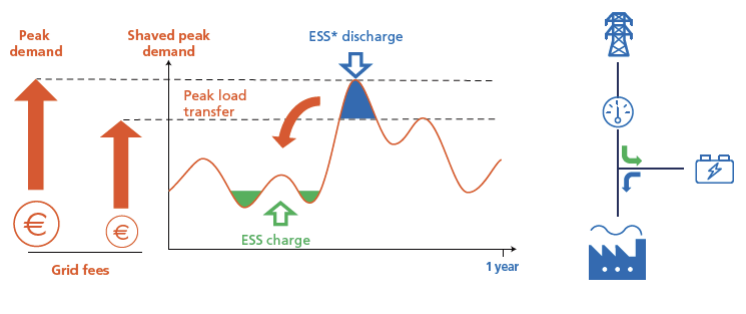
\includegraphics[width=0.98\linewidth]{images/Reduktion_Netzbezugsleistung.png}

\begin{itemize}
    \item Minimieren der monatlichen Leistungsspitze
    \begin{itemize}
        \item Reduziert die Kosten für größere Verbraucher mit Leistungstarif
    \end{itemize}
\end{itemize}



\subsubsection{... durch Wärmepumpe und Betterie}

\begin{itemize}
    \item Jahresdauerlinie Netzbezug
    \begin{itemize}
      \item PV-Leistung 7{,}2 kWp, Stromverbrauch ca. 7'200 kWh/a
      \item Mit einer 6 kWh / 6 kW Batterie können die Netzbezugsspitzen deutlich reduziert werden
    \end{itemize}
\end{itemize}

\vspace{0.15cm}

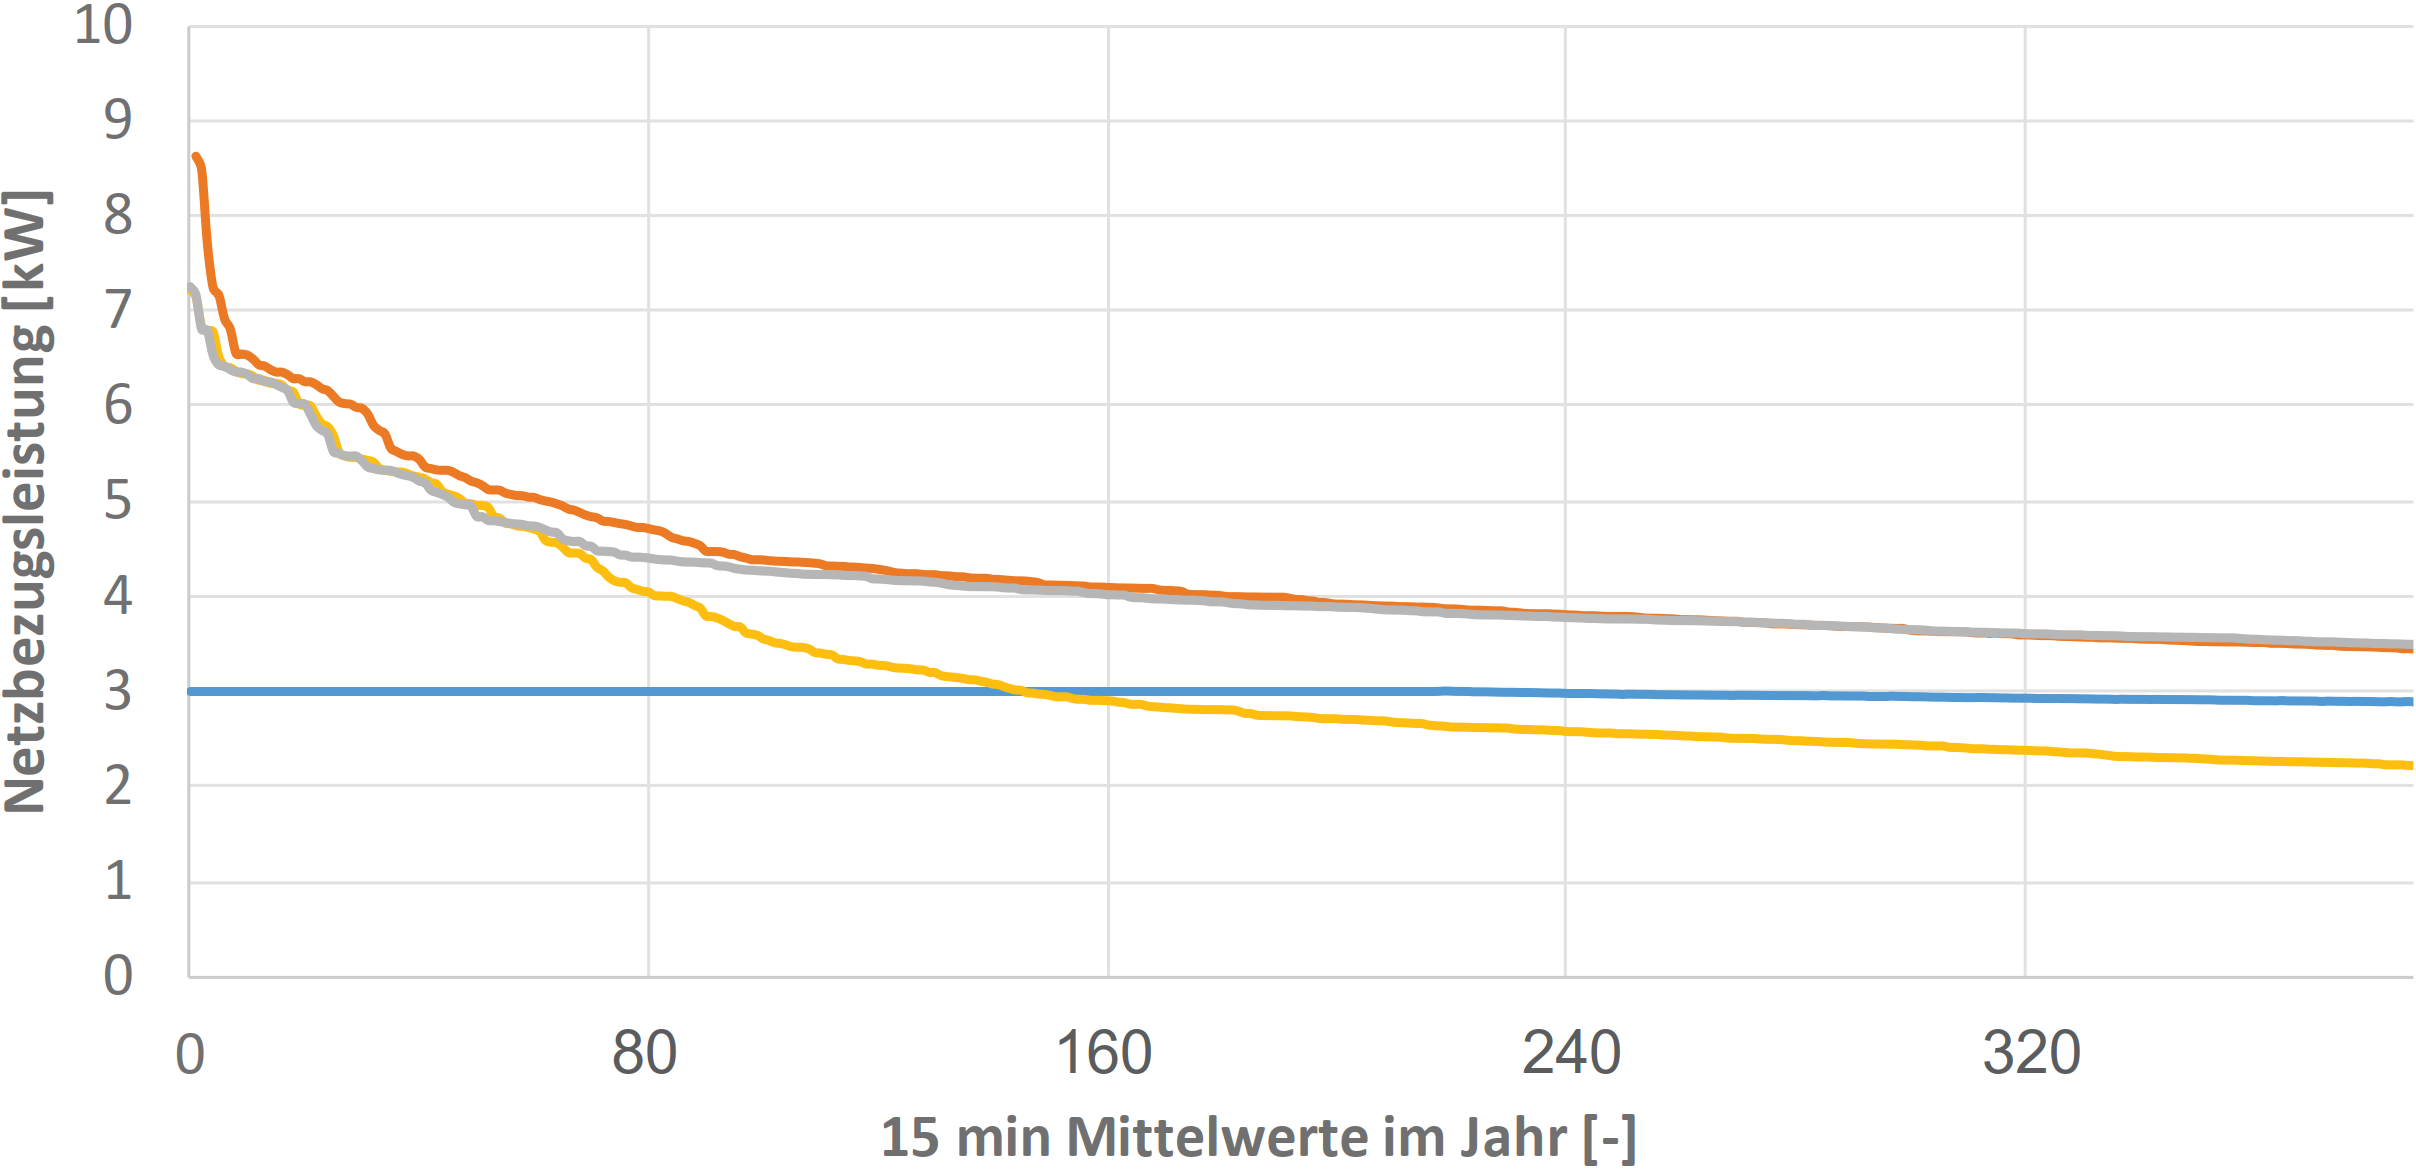
\includegraphics[width=0.98\linewidth]{images/Durch_Wärmepumpen_und_Batterien_1.png}

\vspace{0.15cm}

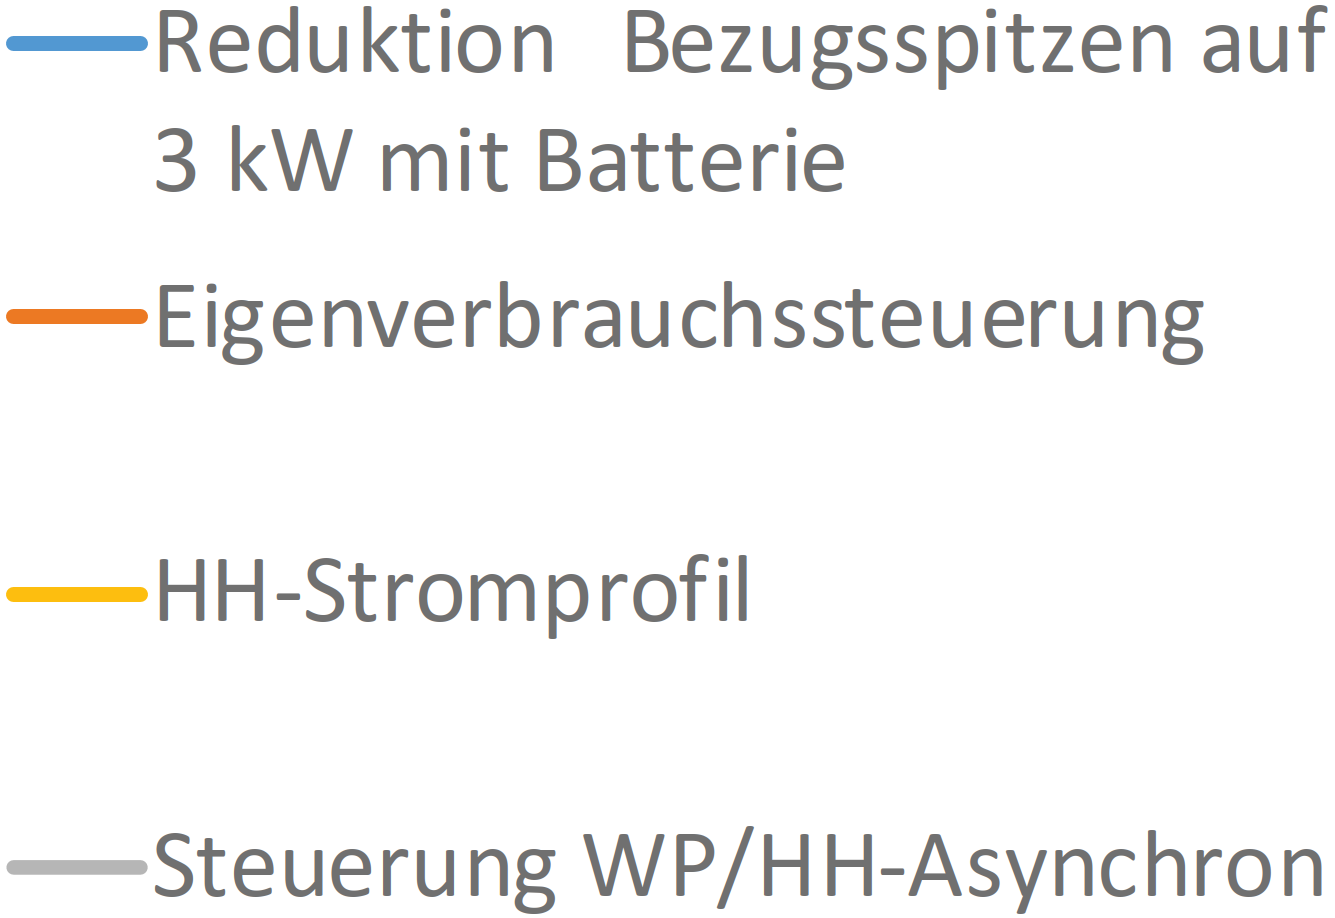
\includegraphics[width=0.35\linewidth]{images/Durch_Wärmepumpen_und_Batterien_2.png}



\subsection{Reduktion von Einspeiseleistung}

\subsubsection{Konventionelle Speicherung}
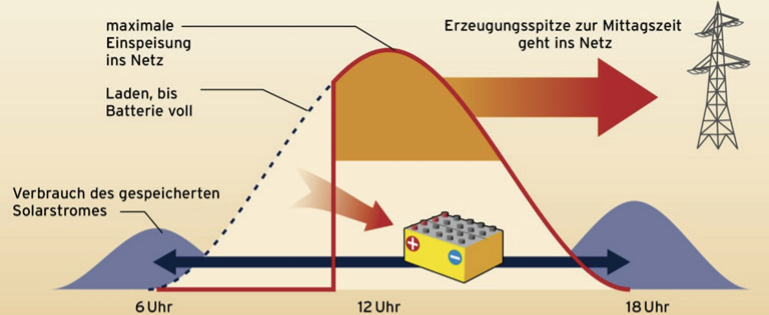
\includegraphics[width=0.98\linewidth]{images/Konventionelle_Speicherung.png}

\subsubsection{Netzoptimierte Speicherung}
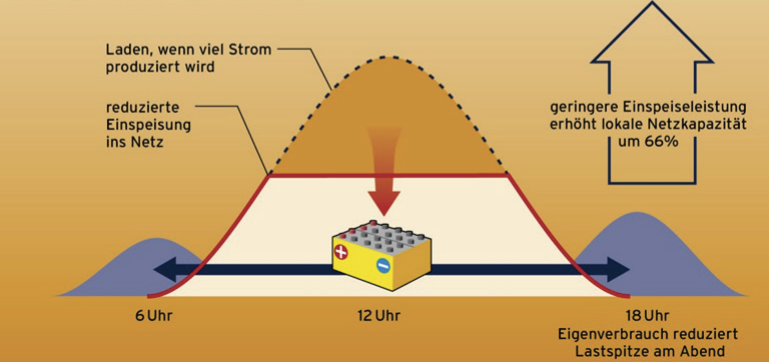
\includegraphics[width=0.98\linewidth]{images/Netzoptimierte_Speicherung.png}



\subsection{Reduktion der Netzeinspeiseleistung}

\begin{itemize}
    \item Verschiedene Betriebsstrategien
    \begin{itemize}
      \item Jahresmittlerer Tagesgang der Einspeiseleistung (links) und Jahresdauerlinien der Einspeiseleistung (rechts)
      \item PV-Leistung 5 kWp, nutzbare Speicherkapazität 5 kWh
    \end{itemize}
\end{itemize}

\vspace{0.15cm}

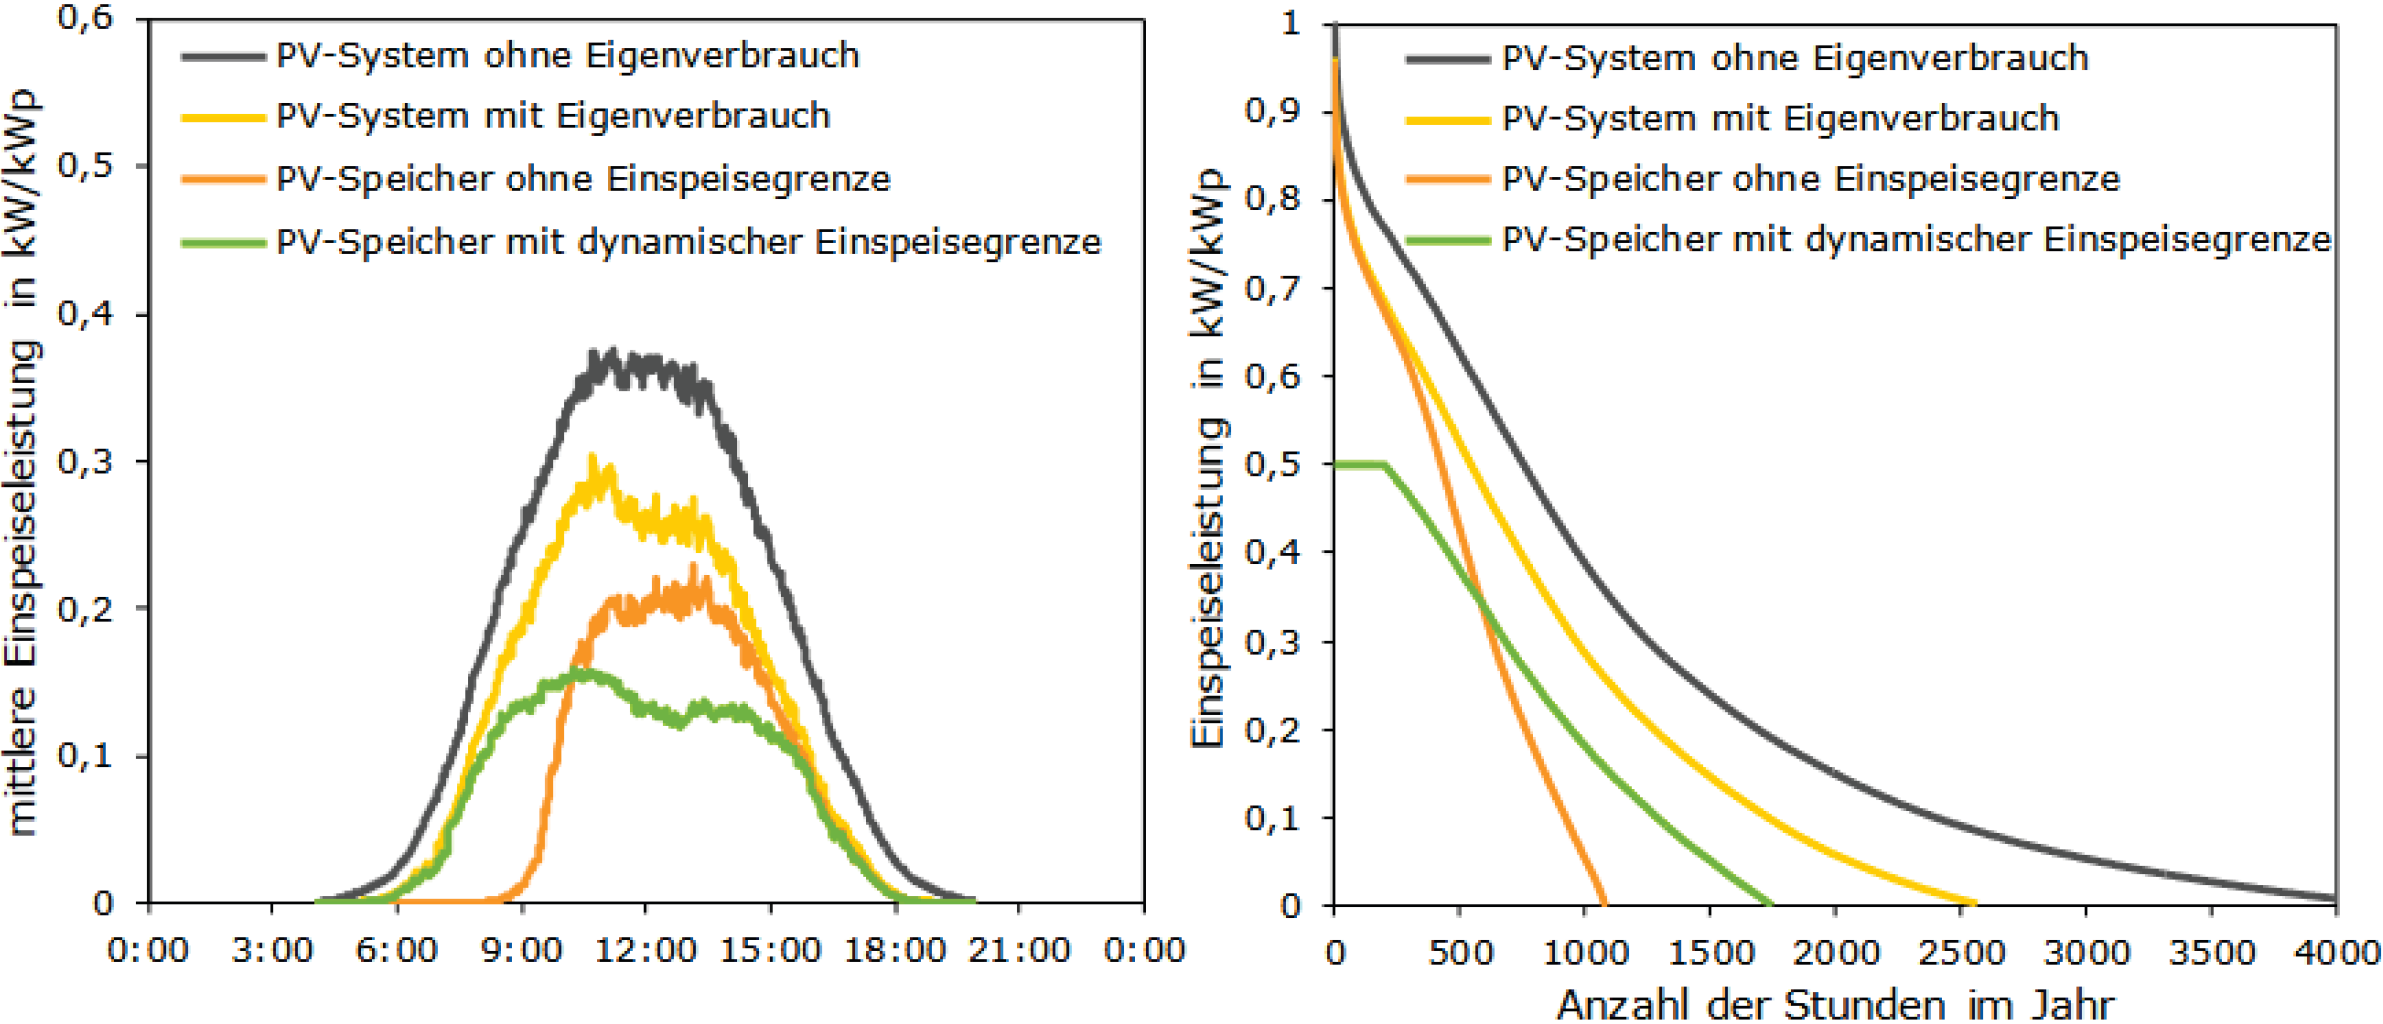
\includegraphics[width=0.98\linewidth]{images/Reduktion_der_Netzeinspeiseleistung.png}

\subsubsection{Beispiel mit 8 kWp}
\begin{itemize}
    \item Begrenzung der Einspeiseleistung am Netzverknüpfungspunkt auf 
    50 \% der nominalen PV-Generatorleistung (4 kWp)
\end{itemize}

\begin{minipage}[c]{0.49\columnwidth}
    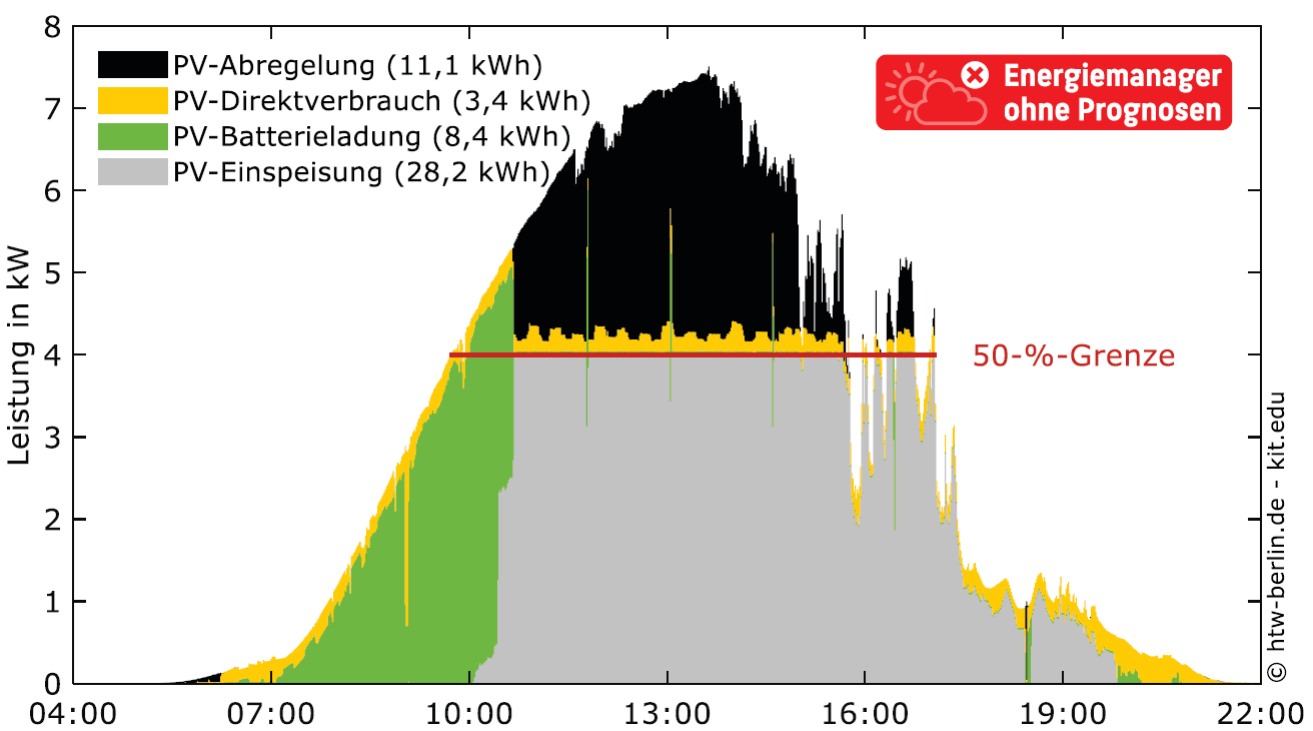
\includegraphics[width=0.98\columnwidth]{images/Reduktion_der_Netzeinspeiseleistung_Beispiel_1.png}
\end{minipage}
\hfill
\begin{minipage}[c]{0.49\columnwidth}
    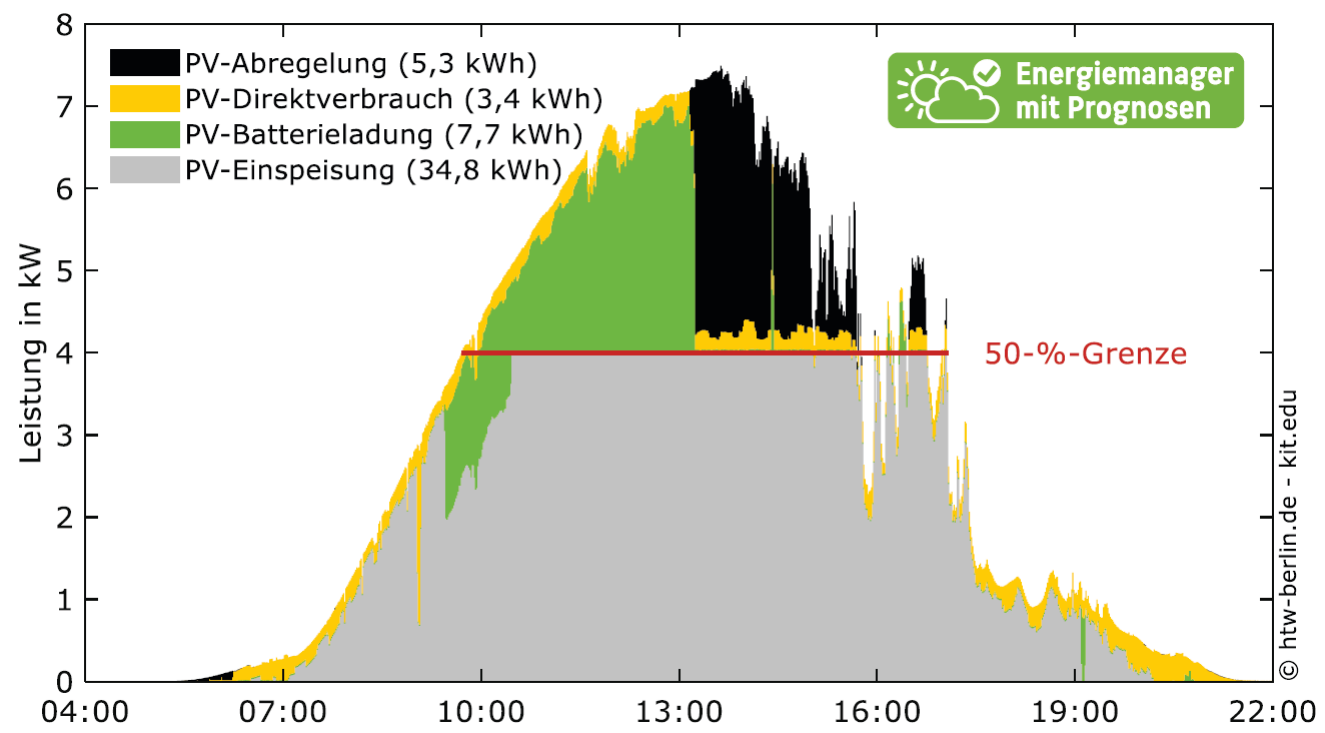
\includegraphics[width=0.98\columnwidth]{images/Reduktion_der_Netzeinspeiseleistung_Beispiel_2.png}
\end{minipage}


\subsubsection{Abregelungsverluste}

Die resultierende Höhe der \textbf{Abregelungsverluste} hängt unter anderem von folgender Eigenschaften der PV-Speichersysteme ab:
\begin{itemize}
  \item Nutzbare Speicherkapazität des Batteriespeichers
  \item Nennleistung des Wechselrichters und des Batteriespeichers
  \item Wechselrichter- und Batteriewirkungsgrad
  \item Güte der Prognosen (PV-Leistung und elektrische Last)
  \item Güte der Ladezustandsbestimmung
  \item Qualität des Optimierungsalgorithmus
  \item Qualität der Regelung zum schnellen Ausgleich von Prognosefehlern
  \item Dauer bis zur nächsten Aktualisierung des Ladefahrplans
  \item Abregelungsverhalten (Möglichkeit der stufenlosen Abregelung)
\end{itemize}


\subsubsection{Prognosebasierte Steuerung mit selbstlernendem Algorithmus}

\begin{tabular}{|l|c|c|c|}
    \hline
     & S1 & S2 & S3\\
    \hline
    DC-Zykleneffizienz & 91{,}5\,\% & 92{,}1\,\% & 92{,}6\,\% \\
    \hline
    Gesamtsystemeffizienz & 91{,}7\,\% & 90{,}4\,\% & 88{,}6\,\% \\
    \hline
    Autarkiegrad & 47{,}4\,\% & 47{,}8\,\% & 47{,}4\,\% \\
    \hline
\end{tabular}

\vspace{0.15cm}

S1: Normale Steuerung\\
S2: Leistungsreduzierung auf 70\,\%\\
S3: Leistungsreduzierung auf 50\,\%

\subsection{Betriebsstrategien zur Verlängerung der Lebensdauer}

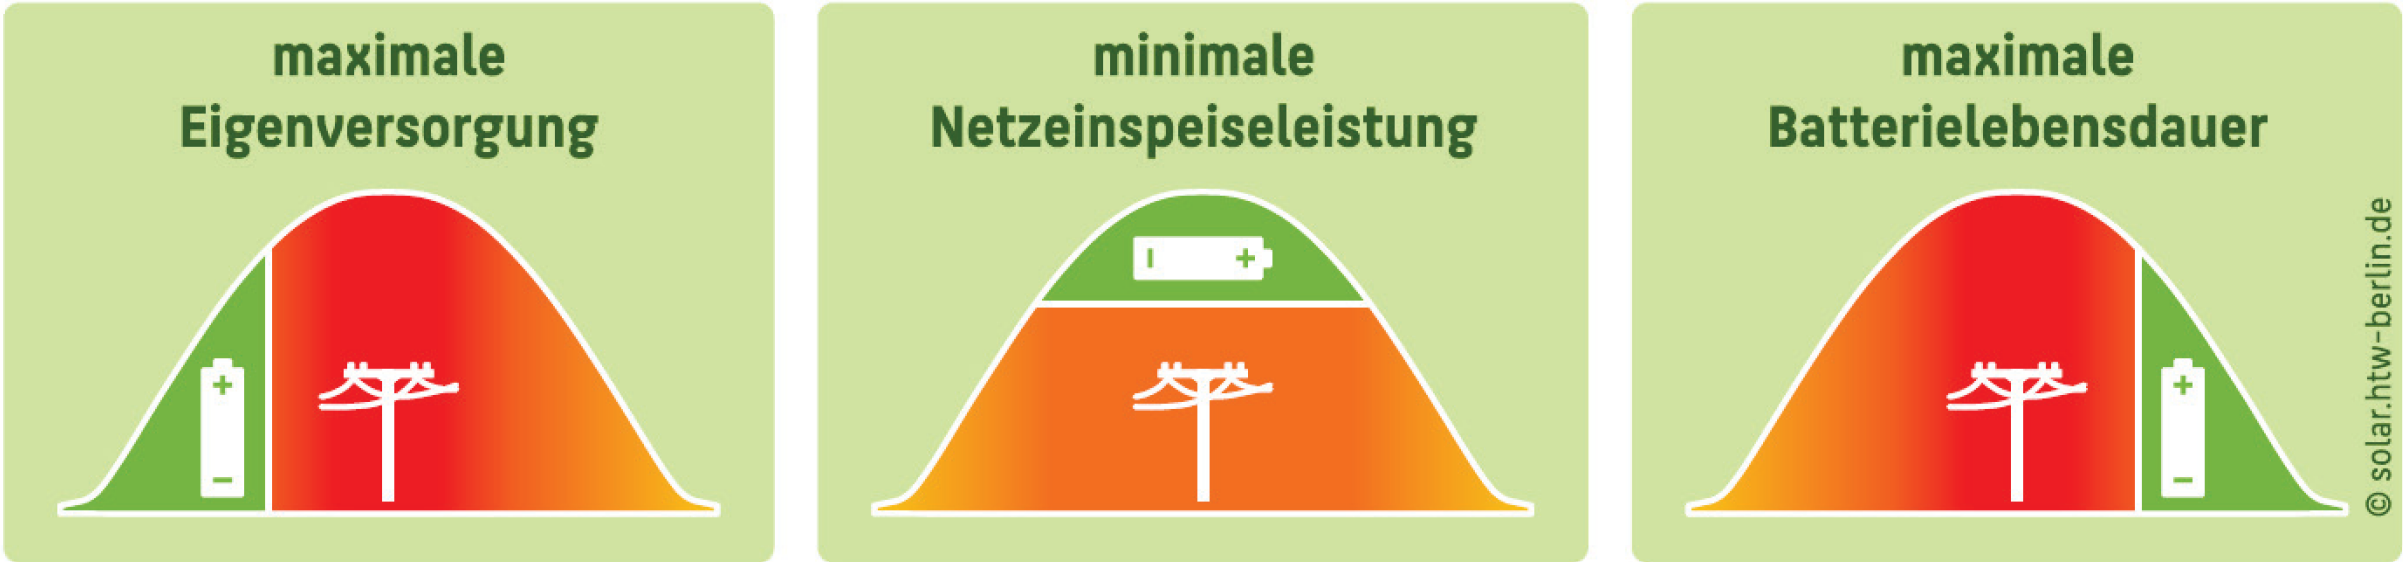
\includegraphics[width=0.98\columnwidth]{images/Betriebsstrategie_zur_Verlängerung_der_Lebensdauer.png}

\vspace{0.15cm}

\begin{tabular}{@{}lll@{}}
\toprule
\textbf{Ladestrategie} & \textbf{Zeitpunkt}       & \textbf{Standzeit $>$ 90\,\% Ladezustand} \\ \midrule
Frühzeitig              & Vormittags                  & 99\,h                                     \\
Prognosebasiert         & Mittags                  & 72\,h                                     \\
Prognosebasiert         & Nachmittags              & 43\,h                                     \\ \bottomrule
\end{tabular}

\textbf{Hinweis:} Je kürzer die Lithium-Batterie vollständig geladen ist, desto langsamer altert sie.




\subsection{Elektromobilität als Heimspeicher}
\begin{itemize}
    \item Als Verbraucher / steuerbare Last
    \begin{itemize}
      \item Integration ins Lastmanagement / Energiemanagementsystem (EMS)
    \end{itemize}
    \item Als Stromspeicher
    \begin{itemize}
      \item Bidirektionales Laden / Vehicle-to-Home (V2H)
    \end{itemize}
  \end{itemize}

























        \section{Industrie- und Gewerbegrossspeicher}

\subsection{Batteriespeicher in Gewerbe}

\subsubsection{Motivation von gewerblichen Kunden für eine Solarbatterie}

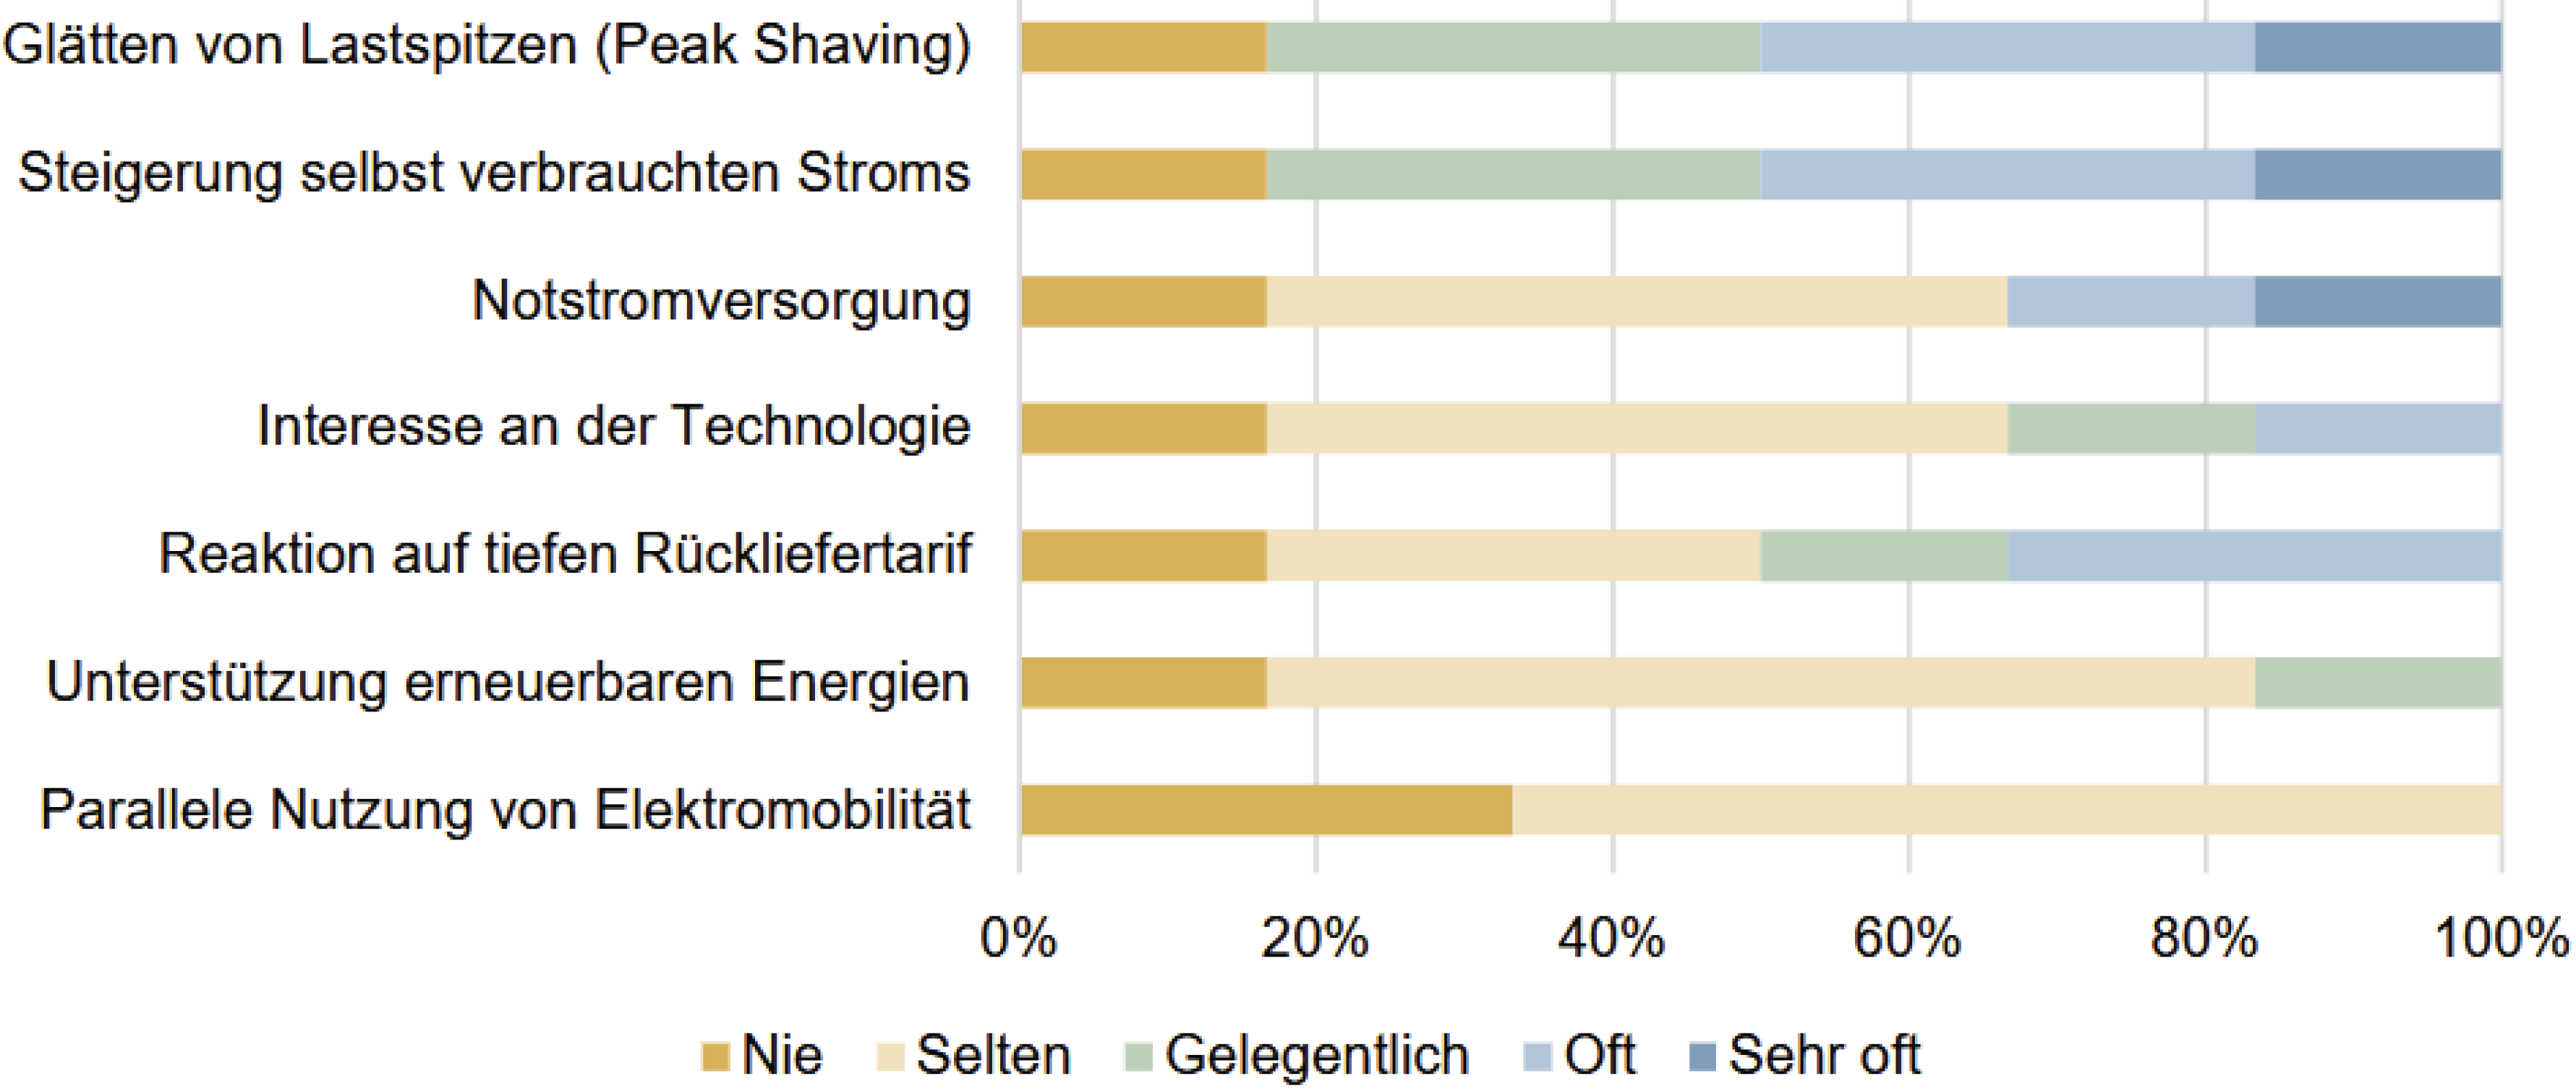
\includegraphics[width=0.98\columnwidth]{images/Batteriespeicher_im_Gewerbe.png}



\subsection{Quartier- und Grossspeicher}

\begin{itemize}
  \item \textbf{Betrieb häufig durch Netzbetreiber}
  
  \item \textbf{Motivation / Möglichkeiten}
  \begin{itemize}
    \item Vermarktung "Eigenverbrauch" an Kunden
    \item Vermeidung von Netzengpässen (Verschiebung von Last- und Einspeisespitzen)
    \item Bereitstellung von Regelleistung (mind. 1 MW für Primärregelleistung, mind. 5 MW für Sekundärregelleistung, auch mit mehreren Speichern möglich)
    \item Für Verteilnetzbetreiber: Reduzierung der Kosten gegenüber vorgelagertem Netz (Leistungspreis) durch Peak-Shaving
    \item Flexibilität bei Energiebeschaffung am Strommarkt (Termin-, Spot-, Intradaymarkt)
    \item Fahrplanmanagement, Bilanzausgleich zur Vermeidung von Strafzahlungen
    \item Unterstützung Spannungshaltung durch Blindleistungseinspeisung (durch Wechselrichter)
    \item Dynamische Anpassung bei Kurzschlusssituationen (Kompensierung von Leistungstransienten und Vermeidung von Überstromsituationen z.\,B. bei Schaltvorgängen)
  \end{itemize}
\end{itemize}


\subsubsection{Beispiel EKZ}



\subsubsection{Beispiel EWJR}




\subsection{Batteriespeicher in Industrie und Gewerbe}
\begin{itemize}
    \item Motivation: Reduktion von Energiekosten, Netzstabilisierung
    \item Multi-Use Konzepte: Eigenverbrauch, Peak-Shaving, Vermarktung von Flexibilität
\end{itemize}

\subsection{Quartier- und Grossspeicher}
\begin{itemize}
    \item Anwendung durch Netzbetreiber: Netzengpässe vermeiden, Regelleistung bereitstellen
    \item Unterstützung von Bilanzkreisausgleich, Fahrplanmanagement
    \item Beispiele:
    \begin{itemize}
        \item EKZ: 18 MW Leistung, 7.5 MWh Kapazität
        \item EWJR: Erweiterung auf 6 MW / 6 MWh
    \end{itemize}
\end{itemize}

\subsection{Regelleistung}
\begin{enumerate}
    \item Primärregelleistung (30 Sekunden)
    \item Sekundärregelleistung (5 Minuten)
    \item Tertiärregelleistung (15 Minuten)
\end{enumerate}



























        \columnbreak
\section{Inselsysteme}

\begin{itemize}
    \item Einsatz in abgelegenen Regionen (z.B. Berghütten, Inseln)
    \item Typen
        \begin{itemize}
            \item PV-Inselsysteme
            \item PV-Pumpensysteme
            \item Mikronetze
        \end{itemize}
    \item Dimensionierung:
    \begin{itemize}
        \item Ermittlung Strombedarf
        \item Auslegung Batteriespeicher (Autonomiezeit, Kapazität)
        \item Dimensionierung Solargenerator auf schwächsten Monat
    \end{itemize}
\end{itemize}
%\begin{comment}
\subsubsection{Aufbau Inselsysteme}

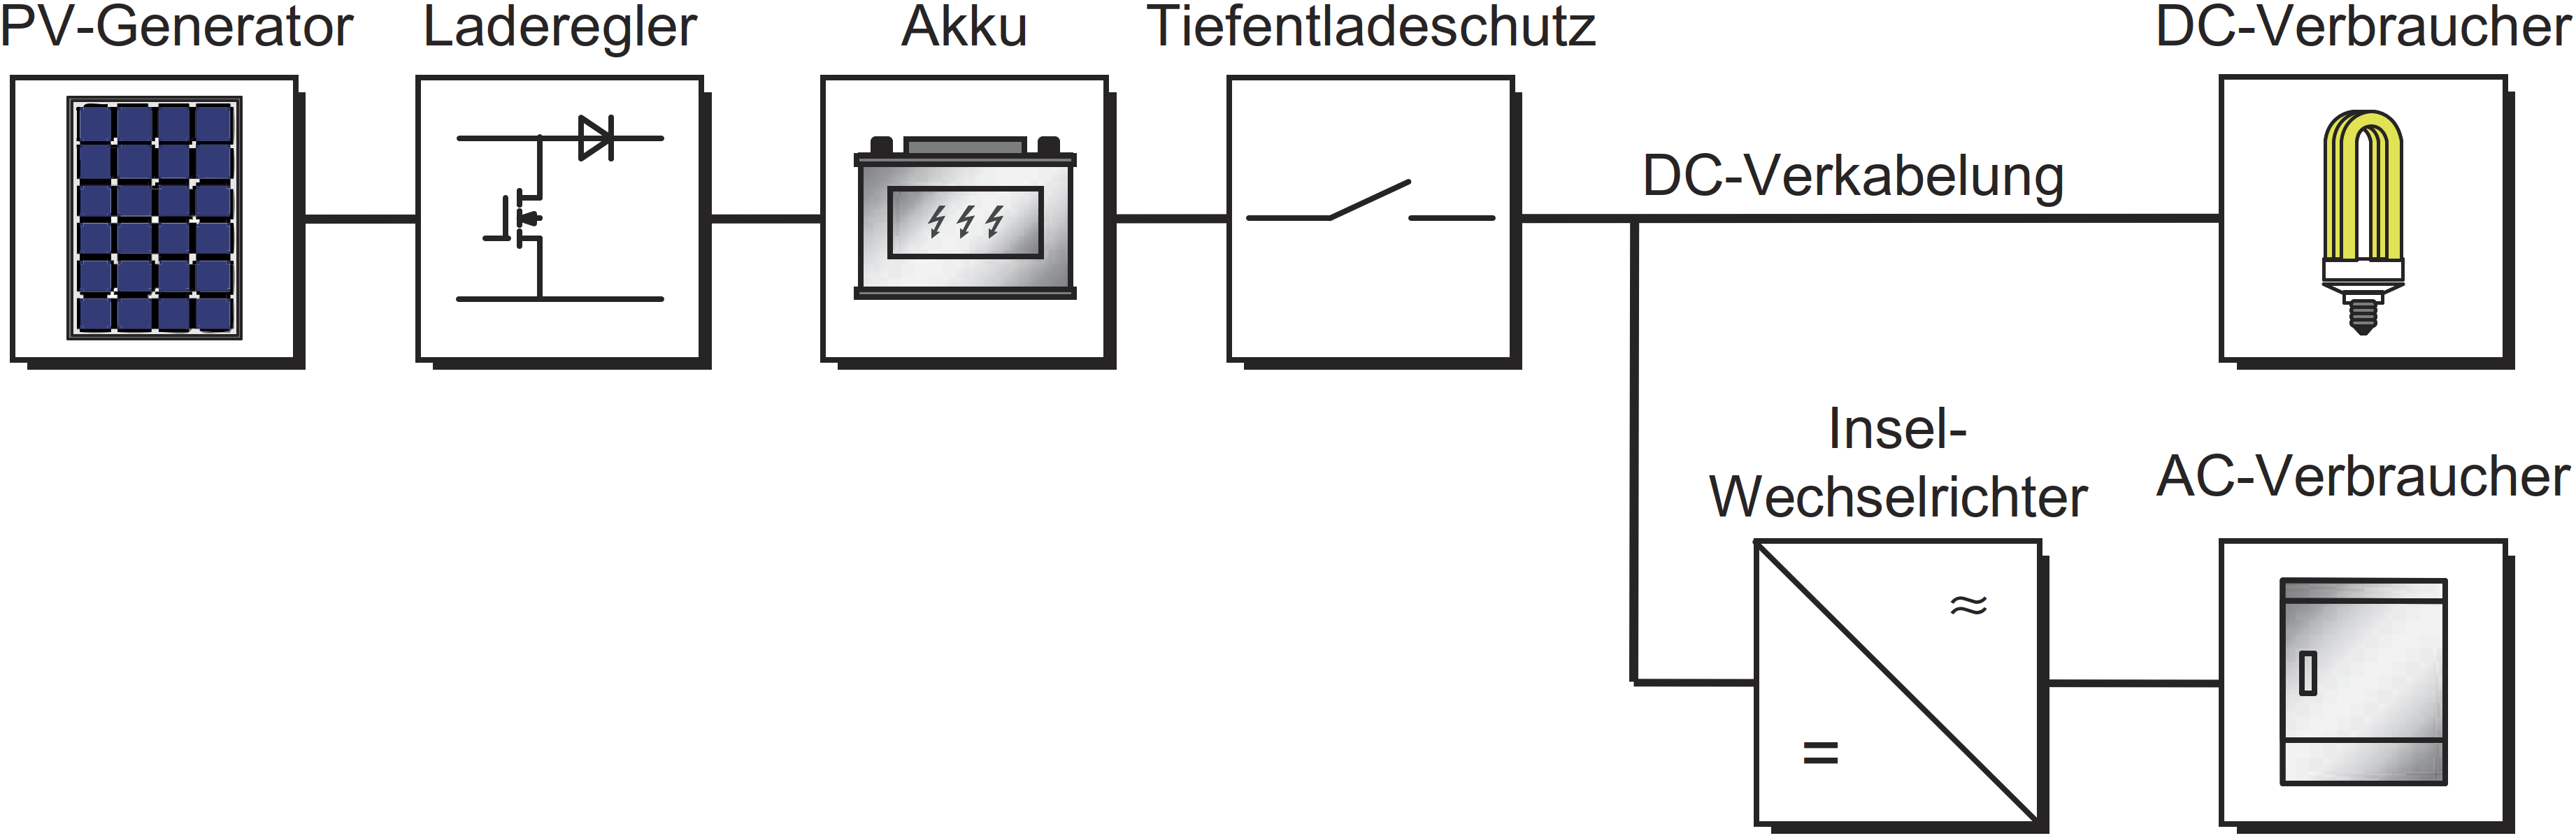
\includegraphics[width=0.98\linewidth]{images/Inselsysteme.png}
%\end{comment}

\subsection{Dimmensionierung}

\subsubsection{Ermittlung Stromverbrauch}

\begin{itemize}
    \item Nutzungsprofil: Saison/Monate, Anzahl Tage (z.B. Wochenendhaus)
    \item Bedarfstabelle täglicher Verbrauch
\end{itemize}

\subsubsection{Dimmensionierung Batteriespeicher}

\begin{itemize}
    \item Wahl Batterietyp: z.B. Blei (seltene Nutzung / wenige Zyklen) oder Lithium-Ionen (tägliche Nutzung)
    \item Gewünschte Autonomiezeit in Tagen (gewünschte Versorgungssicherheit)
    \item Maximale Last
\end{itemize}

\vspace{0.15cm}

$
\boxed{
C_{\mathrm{N}} = \frac{W \cdot N_{\mathrm{A}}}{U_{\mathrm{N}} \cdot \eta_{\mathrm{S}} \cdot DOD \cdot SOH_{\mathrm{min}}}
}
\quad \text{oder} \quad
\boxed{
C_{\mathrm{N}} = \frac{P_{\mathrm{max}} \cdot t_{\mathrm{disc}}}{U_{\mathrm{N}}}
}
$

$\boxed{\text{C-Rate} = \frac{P}{W}}$
\quad
$\boxed{R_{\mathrm{eig}} = \frac{W_{\mathrm{eig}}}{W_{\mathrm{PV,AC}}}}$
\quad
$\boxed{R_{\mathrm{Autarkie}} = \frac{W_{\mathrm{eig}}}{W_{\mathrm{ges}}}}$
\quad
$\boxed{R_{\mathrm{PV}} = \frac{W_{\mathrm{PV,AC}}}{W_{\mathrm{ges}}}}$


\renewcommand{\arraystretch}{1.2}
\begin{tabular}{@{} l p{6.5cm} l @{}}
    $[C_{\mathrm{N}}]$           & Nennkapazität der Batterie \dotfill                                  & $\mathrm{Ah}$ \\
    $[W]$                        & Elektrischer Energiebedarf pro Tag \dotfill                          & $\mathrm{Wh/d}$ \\
    $[N_{\mathrm{A}}]$           & Autonomiezeit (Tage ohne Nachladung) \dotfill                        & $\mathrm{d}$ \\
    $[P_{\mathrm{PV}}]$          & Nennleistung des PV-Generators \dotfill                              & $\mathrm{W_p}$ \\
    $[H_{i,\mathrm{gen}}]$       & Monatsmittlere Tagesstrahlungssumme auf geneigte Fläche \dotfill     & $\frac{\mathrm{Wh}}{\mathrm{31 \cdot d \cdot m^2}}$ \\
    $[\eta_{\mathrm{S}}]$        & Wirkungsgrad der Ausspeicherung \dotfill                             & $-$ \\
    $[DOD]$                      & Entladetiefe (Depth of Discharge) \dotfill                           & $-$ \\
    $[SOH_{\mathrm{min}}]$       & Minimaler State of Health / Gesundheitszustand \dotfill              & $-$ \\
    $[P_{\mathrm{max}}]$         & Maximale gleichzeitige Verbraucherleistung \dotfill                  & $\mathrm{W}$ \\
    $[k]$                        & Sicherheitsfaktor \dotfill                                           & $-$ \\
    $[\eta_{\mathrm{Sys}}]$      & Systemwirkungsgrad \dotfill                                          & $-$ \\
    $[U_{\mathrm{N}}]$           & Systemspannung \dotfill                                              & $\mathrm{V}$ \\
    $[SOC]$                      & Ladezustand in \% \dotfill                                           & \% \\
    $[\text{C-Rate}]$            & Entladerate ($P/W$) \dotfill                                         & $\mathrm{h^{-1}}$ \\
    $[t_{\mathrm{disc}}]$        & Minimale Entladezeit \dotfill                                       & $\mathrm{h}$ \\
    $[R_{\mathrm{eig}}]$         & Eigenverbrauchsquote \dotfill                                        & \% \\
    $[R_{\mathrm{Autarkie}}]$    & Autarkiegrad \dotfill                                                & \% \\
    $[R_{\mathrm{PV}}]$          & PV-Ertragsverhältnis \dotfill                                       & \% \\
\end{tabular}


\subsubsection{Faustregeln für Kapazitätsauslegung}
Zwischen 100\% - 150\% der PV-Leistung\\
oder zwischen 90\% - 120\% des Stromverbrauches\\
Es sollte ein gerundeter Wert gewählt werden (Reale Welt und so)\\
Autarkie und Eigenverbrauch werden bei Dimensionierung grösser als eines Tagesspeichers nicht grösser.\\
Die C-Rate soll mind. 0.3kW pro kWh Ladeleistung betragen.\\
\subsubsection{Dimmensionierung Solargenerator}

\begin{itemize}
    \item Wird auf den Strahlungsschwächsten Monat ausgelegt!
\end{itemize}

\vspace{0.15cm}

$\boxed{P_{\text{PV}}= \frac{W \cdot k \cdot 1'000 \frac{\textbf{W}}{\textbf{m$^2$}}}{H_{i,\text{gen}} \cdot \eta_{\text{Sys}}}}$



\subsubsection{Mikronetze}

\begin{itemize}
    \item Meist als Hybridsystem mit AC-Kopplung der Erzeuger und Verbraucher
    \item Speicherdimensionierung sehr individuell je nach Energieerzeugung, Verbrauchern etc.
    \item Bei größeren Systemen häufig Hybridbatterie als »Leistungsbatterie« (z.B. Lithium) und »Energiebatterie« (z.B. Redox-Flow)
\end{itemize}

\subsection{Autarkiegrad}
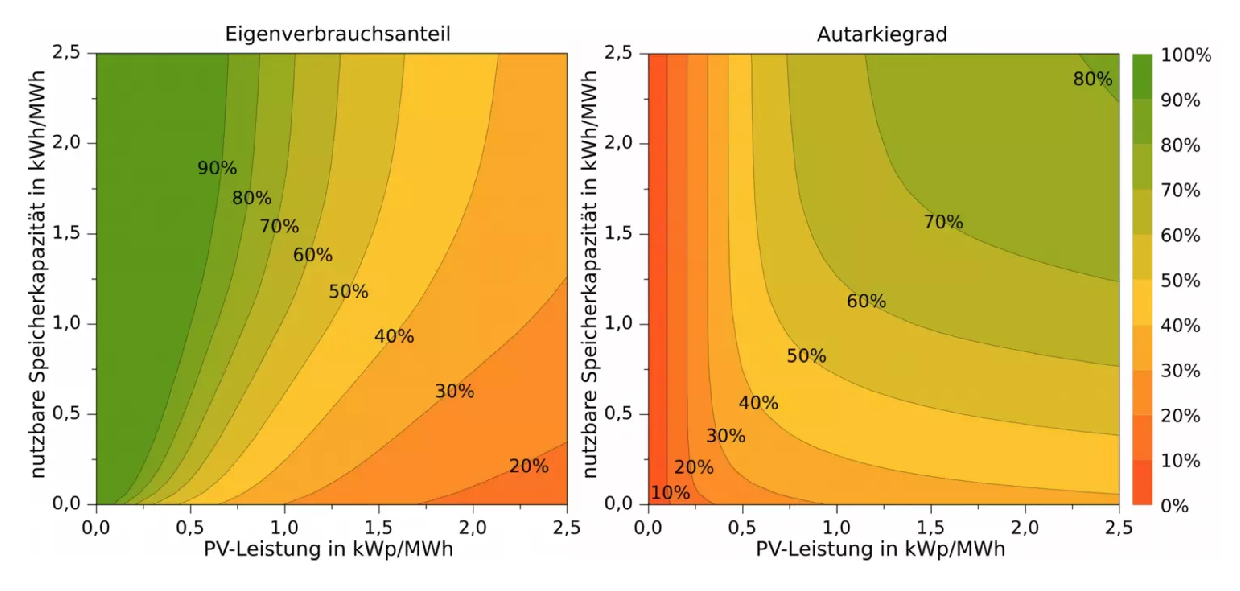
\includegraphics[width=0.98\linewidth]{images/Autarkiegrad.pdf}\\
\begin{itemize}
    \item Immer Systemeffizienz und Eigenverbrauchquote bei Auslegung beachten.
    \item Systemeffizienz wird beinflusst durch:
    \item Umwandlungswirkungsgrade (AC-DC)
    \item DC - Verluste
    \item Standby-Verbrauch
\end{itemize}
        \section{I/U-Kennlinienmessung}

\subsection{Kennlinienmessung - Fehlerbilder}

\subsubsection{Hoher Serienwiderstand}

\begin{itemize}
    \item Korrosion Lötverbindung
    \item Unterbruch von Lötverbindungen
    \item Defekte Zellverbinder
    \item Kontaktfehler in der Anschlussdose
\end{itemize}


\subsubsection{Niedriger Shuntwiderstand}

\begin{itemize}
    \item Shunts / Hot Spots
    \item Heterogener Transparenzverlust
    \item Heterogene Glaskorrosion
    \item Heterogene Delamination
    \item Teilverschattung des Moduls
\end{itemize}


\subsubsection{Knickpunkt}

\begin{itemize}
    \item Gebrochene Zellen
    \item Heterogener Transparenzverlust
    \item Heterogene Glaskorrosion
    \item Heterogene Delamination
    \item Defekte Zellverbinder
    \item Verschattung
\end{itemize}


\subsubsection{Änderung der Neigung}

\begin{itemize}
    \item Potential induzierte Degradation (PID)
    \item Heterogene Korrosion der AR-Beschichtung
\end{itemize}


\subsubsection{Niedriger Isc}

\begin{itemize}
    \item EVA Verfärbung (Browning)
    \item Delamination
    \item Transparenzverlust / Gleichmäßige Verschmutzung
    \item Glaskorrosion / Korrosion der AR-Beschichtung
    \item Gebrochene Zellen
    \item (Licht induzierte Degradation, LID)
\end{itemize}


\subsubsection{Niedriger Uoc}

\begin{itemize}
    \item Kurzgeschlossene oder falsch angeschlossene Bypass-Diode
    \item Degradation der Passivierung
    \item PID, LID
    \item Kurzgeschlossene Zelle
    \item Verschattung
\end{itemize}



        \section{Fehler}

\subsection{Visuelle Inspektion}

\begin{itemize}
    \item Modulvorderseite
    \begin{itemize}
      \item Delamination, Yellowing, Browning, Blasen, Glasbruch, Verschmutzung, \ldots
    \end{itemize}
    
    \item Zellen
    \begin{itemize}
      \item Gebrochene Zellen, Zellrisse, Schneckenspuren, Verfärbung AR-Beschichtung, \ldots
    \end{itemize}
    
    \item Zellverbinder
    \begin{itemize}
      \item Korrosion, Oxidation, Hot Spots, Unterbrüche, \ldots
    \end{itemize}
    
    \item Rahmen
    \begin{itemize}
      \item Verbogen, gebrochen, verkratzt, schief, \ldots
    \end{itemize}
    
    \item Modulrückseite
    \begin{itemize}
      \item Delamination, Blasen, Kratzer, Yellowing, Brandflecken, \ldots
    \end{itemize}
    
    \item Anschlussdose
    \begin{itemize}
      \item Lose, (Oxidation, Korrosion, fehlende Verbinder), \ldots
    \end{itemize}
    
    \item Kabel / Stecker
    \begin{itemize}
      \item Ablösung, brüchig, freiliegende elektrische Teile, \ldots
    \end{itemize}
  \end{itemize}
  

  \subsection{Fehler bei PV-Modulen}

  \begin{itemize}
    \item Verfärbung
    \item Delamination
    \item Rückseitenfolie
        \begin{itemize}
            \item Delamination, Rissbilidung, Chalking
        \end{itemize}
    \item Brandflecken
    \item Glasbruch
    \item Anschlussdose
    \item Verschmutzung
    \item DC-Verbinder und Kabel
    \item Montagesystem
    \item Verschattung
    \item Wechselrichter
    \begin{itemize}
        \item Installationsfehler
        \item Defekte $\rightarrow$ Monitoring
    \end{itemize}
  \end{itemize}













        \input{sections/57_Normen.tex}
        %\input{sections/99_Mustercodes.tex}
    \end{layout}
\end{document}
